 \documentclass[12pt,a4paper]{report}
%preamble
\usepackage{titlesec}
\usepackage{amsmath}
\usepackage{acronym}
\usepackage{longtable}
\usepackage{tabularx}
% Adjust the spacing before and after chapters and sections
\titlespacing*{\chapter}{0pt}{-20pt}{20pt}  % {left}{before}{after}
\titlespacing*{\section}{0pt}{-10pt}{10pt}  % {left}{before}{after}
%\usepackage[colorlinks=true]{hyperref}
\usepackage{hyperref}
%\hypersetup{
   %colorlinks=true,
   % urlcolor=blue, % Sets the URL color to blue
%}
\usepackage{graphicx}
\usepackage{tabularx}
\usepackage{acronym}
\usepackage{booktabs}
\usepackage[table]{xcolor} % for \cellcolor
\usepackage{graphicx}
\usepackage{float}
\usepackage{caption}
\usepackage{subcaption}
\usepackage{placeins}
\usepackage{multirow} 
%\usepackage{rotating}
\usepackage{amsmath}
\usepackage{hyperref}
\usepackage{setspace} \doublespacing
%\usepackage{natbib} % for ieee style comment out this but for apa style uncomment
\newtheorem{theorem}{Theorem}
%\usepackage{amsmath,amssymb,amsfonts}
%\usepackage{mathtools}
%\usepackage{pdflscape,multicol,multirow}
%\usepackage[T1]{fontenc}
%\usepackage[utf8]{inputenc}
%\usepackage{apacite}
%\pagestyle{plain}
%\usepackage{multirow}
%\usepackage[table]{xcolor}
%\usepackage{caption}
%\usepackage{mathptmx}
%\usepackage{float}
%\usepackage{courier}
%\usepackage{multirow}
%\newtheorem{definition}{Definition}[section]
%\usepackage[toc,page]{appendix}
%\usepackage[usenames, dvipsnames]{color}
%\usepackage{tabularx}
%\usepackage{adjustbox}
%\usepackage{verbatim}
%\usepackage {hyperref}
%\usepackage{titlesec}
%\usepackage{graphicx}
%graphicspath{ {figures/} }
%\usepackage{array}
%\usepackage{comment}
%\graphicspath{ {figures/} 
	%\renewcommand{\listtablename}{Tables}

%\usepackage{lipsum}
%\usepackage{fixmath}
%\usepackage{pdflscape}
%\usepackage{longtable} % for tables that span multiple pages
%\numberwithin{equation}{section}
%\renewcommand{\chaptername}{CHAPTER}{\Large}
%\large \titleformat{\chapter}[display]
%{\vspace{0mm}\filcenter}
%{\filcenter \LARGE\bfseries
	%\chaptertitlename\ \justwords{\thechapter}}
%{1ex}
%{\vspace*{0ex}\filcenter\Huge\bfseries}
%\def\justwords#1{\ifcase#1 \or ONE\or TWO\or %THREE\or FOUR \or FIVE\fi}
%\usepackage{graphicx}
\usepackage{setspace}
\usepackage{nomencl}
\usepackage{enumerate}
\usepackage{adjustbox}
\usepackage{caption}
\usepackage{subcaption}
\usepackage{enumitem}
\usepackage{pdfpages}
\usepackage{titlesec} % For title formatting
\titleformat{\chapter}[display]
  {\normalfont\filcenter\Huge\bfseries}
  {\MakeUppercase{\chaptertitlename} \thechapter}{20pt}{\Huge}
  % Custom command for centered abstract title
\newcommand{\abstracttitle}{
  
}
%\titleformat{\chapter}[display]
 % {\normalfont\filcenter\Huge\bfseries}
  %{\chaptertitlename\ \thechapter}{20pt}{\Huge}

%\makenomenclature
%\usepackage[authoryear]{natbib}
%\renewcommand{\bibname}{REFERENCES}
%\renewcommand{\refname}{REFERENCES}
%\renewcommand{\bibsection}{\section*{\hspace{4cm}REFERENCES}}
%\renewcommand{\listtablename}{LIST OF TABLES}
%\usepackage{geometry}
\usepackage[left=2.0cm,top=2.9cm,right=2.0cm,bottom=2.5cm]{geometry} 
%\providecommand{\printnomenclature}{\printglossary}
%\providecommand{\makenomenclature}{\makeglossary}
%\usepackage{nomencl}
%\usepackage{amssymb}
%\usepackage{lipsum}
%\newtheorem{thm}{Theorem}[section]

%%%%%%%%%%%%For table formatting
\usepackage{tocloft}
\renewcommand{\cfttabpresnum}{Table\ }  % adds "Table " before number
\renewcommand{\cfttabaftersnum}{\quad}  % spacing after number
\setlength{\cfttabnumwidth}{3cm}        % adjust spacing if needed



%%%%%%%%%%%%For figures formatting
% --- For Figures ---
\renewcommand{\cftfigpresnum}{Figure\ }
\renewcommand{\cftfigaftersnum}{\quad}
\setlength{\cftfignumwidth}{3cm}


%\newtheorem{theorem}{Theorem}
%\makenomenclature
%\renewcommand{\baselinestretch}{1.5}
%\makeatletter
%\makeatother
%\setlength\parindent{0pt}
%\title{}
%\author{}
%\usepackage{etoolbox}
%\usepackage{natbib}
%\usepackage{hyperref,url}
%\newcounter{bibcount}
%\makeatletter
%\patchcmd{\@lbibitem}{\item[}{\item[\hfil\stepcounter{bibcount}{\thebibcount.}}{}{}
%\setlength{\bibhang}{2\parindent}
%\renewcommand\NAT@bibsetup%
%[1]{\setlength{\leftmargin}{\bibhang}\setlength{\itemindent}{-\parindent}%
	%	\setlength{\itemsep}{\bibsep}\setlength{\parsep}{\z@}}
%\makeatother
%\bibliographystyle{apacite}
		%	\includegraphics[scale=0.8]{logo.jpg}
		%	\begin{center}
			%\textbf{PAN AFRICAN UNIVERSITY}	\\
			%	\textbf{INSTITUTE FOR BASIC SCIENCES, TECHNOLOGY AND INNOVATION}
			%	\end{center}
		%\noindent
		%\rule{\textwidth}{2.8pt}
		%\begin{center}



        \setlength{\parindent}{0pt} % to prevent unwanted indent of paragraphs
  \begin{document}
\begin{titlepage}
\centering
\large{\textbf{TRAJECTORY TRACKING OF QUADROTOR UNMANNED AERIAL VEHICLE USING PARTICLE SWARM OPTIMIZATION BASED ADAPTIVE SUPER TWISTING SLIDING MODE CONTROL}}\\
   \vspace{3cm} 
         \centering
 \textbf{MUSA DAUD }\\
       MT300-0004/2023\\
        \vspace{3cm}
    \textbf{ MASTER OF SCIENCE IN MECHATRONICS} \\
        (Robotics Control Option)\\
       \vspace{5cm}
       A Thesis  submitted to Pan African University Institute for Basic Sciences,Technology, and Innovation in partial fullfilment of the requirement for the Award of the Degree of Master of Science in Mechatronic Engineering\\	
	\vspace{1cm}
\centering
 2025\\

		\end{titlepage}
		\begin{center}
			\noindent\pagenumbering{roman}
		\end{center}
		
		%	\section*{\hspace{4cm}DEDICATION}
		
		%\addcontentsline{toc}{chapter}{DEDICATION}
		
		%\newpage
		%\section*{\hspace{4cm}ACKNOWLEDGMENT}
		%	
		
		%	\addcontentsline{toc}{chapter}{ACKNOWLEDGMENT}
		
		%\newpage
     \begin{center}
        \Large\bfseries DECLARATION
         \vspace{1.5cm}\\
    \end{center}
		%\begin{center}
 %\section*{DECLARATION} 
%\end{center}
\addcontentsline{toc}{section}{DECLARATION}
This thesis is my own work and has not been presented elsewhere for a degree
award in any university.\\
\begin{center}
Signature \dotfill Date \dotfill\\
\end{center} 
\begin{center}
  \textbf{Musa Daud}  
\end{center}  
\tabularnewline \\
	\begin{center}
 MT300-0004/2023\tabularnewline\\  
	\end{center}
		\\
%\vspace{1.5cm} 
This thesis has been submitted for examination with our approval as university supervisors.\\
\begin{center}
Signature \dotfill Date \dotfill 
\end{center}
      \tabularnewline 
			\textbf{\begin{center}
\textbf{ Dr.-Ing. Jackson G. Njiri  } \end{center}
    \begin{center}    JKUAT,Kenya.\end{center}}    \tabularnewline 
			\\
			
     \vspace{1.5cm}\\
      %\vspace{1.5cm}
   Signature \dotfill Date \dotfill \\ 
    %\vspace{0.5cm} 
    \tabularnewline
\begin{center}  \textbf{    Dr. Chala Abdissa Merga }\end{center}
      \begin{center}    Addis Ababa University-Ethiopia\end{center}\tabularnewline \\		
			
		
   

%\newpage
		
	%	\section*{\hspace{5cm}DECLARATION} 
		%\addcontentsline{toc}{chapter}%{DECLARATION}
		%\noindent This research proposal is my own work and has not been presented
		%elsewhere for a degree award. 
		
		%\vspace{1cm}
		
		%\indent %
		%\begin{tabular}{l}
			%Signature...................................................  Date..............................................\tabularnewline \\
			%\textbf{ Eunice Shadrack John}   \tabularnewline 
		%	\textbf{	Reg: No. MS300-0006/2022}\tabularnewline
		%\end{tabular}\\
		%\vspace{1.0cm}
		
		
		%\noindent Declaration by supervisors. \\
		%\vspace{0.4cm}
		
		%\textbf{Declaration by Supervisors}\\This research proposal has been submitted for examination with our approval as University Supervisors. \vspace{1.5cm}
		
		
		%\noindent %
		%\begin{tabular}{l}
			%Signature..................................  Date........................................\tabularnewline 
		%	\textbf{Dr. Anthony Wanjoya}    \tabularnewline 
			
			%Department of Statistics and Actuarial Sciences,\\
		%	Jomo Kenyatta University of Agriculture and Technology, Nairobi, Kenya.
		%\end{tabular}
		%\vspace{1.0cm}
		%\noindent \vspace{0.5 cm}
		
		%\indent %
		%\begin{tabular}{l}
	%Signature..................................  Date........................................\tabularnewline
			%\textbf{Dr. Mutua Kilai}    \tabularnewline 		
		%	Department of Pure and Applied Sciences, Kirinyaga University
		%\end{tabular}
		
		%	\noindent %
		%	\begin{tabular}{l}
			%		Signature..................................  Date........................................\tabularnewline 
			%	\textbf{Prof. Fred Onyango}    \tabularnewline 
			
			%	School of Mathematics, Statistics and Actuarial Science, 
			%	Maseno University
			%	\end{tabular}
		%\vspace{1.0cm}
		%	\noindent \vspace{0.5 cm}
		
		%	\indent %
		%	\begin{tabular}{l}
			%	Signature..................................  Date........................................\tabularnewline
			%	\textbf{Dr. Jane Aduda}    \tabularnewline 		
			%	Department of Statistics and Actuarial Sciences,
			%	Jomo Kenyatta University of Agriculture\\ and Technology, Nairobi, Kenya.
			%\end{tabular}
			
			
			\textbf{\pagebreak{}}
			\section*{\hspace{5cm}DEDICATION}
			%\addcontentsline{toc}{section}{DEDICATION}
   \addcontentsline{toc}{section}{DEDICATION}
			%\addcontentsline{toc}{chapter}{DEDICATION}
            I dedicate this work to my beloved dad Mr. Daud Manhya Kasenga and family, whose unwavering support, love, and encouragement have been my greatest source of strength. A special dedication goes to my dear wife Mrs. Therezia Petro Mathias, my son Riemann Musa Daud whose constant motivation, kindness and belief in my abilities have inspired me to strive for excellence. Your unwavering support has been a guiding light throughout this journey. This thesis is a testament to my family's sacrifices, prayers, and unconditional love. I am forever grateful.
		%This thesis is dedicated to my Almighty God and to my family.
   \textbf{\pagebreak{}}
				\section*{\hspace{5cm}ACKNOWLEDGMENT}
     \vspace{0.5cm}
				\addcontentsline{toc}{section}{ACKNOWLEDGMENT}
I am profoundly grateful to Almighty God for His strength,wisdom and guidance throughout this journey. I sincerely appreciate the African Union (AU) through the Pan African University (PAU) for the scholarship to realize my academic aspirations. I extend my heartfelt gratitude to my research supervisors, Dr.-Ing. Jackson G. Njiri and Dr. Chala Merga Abdissa, for their invaluable guidance and unwavering support. I appreciate the dedicated technicians at Jommo Kenyatta University of Agriculture and Technology (JKUAT) Mr .James Mbugua and Mr .Joseph Kiyondi Matunda for their technical support during the experimental phases. A special thanks goes to Dr. Rehema Ndeda, the mechanical and mechatronic engineering programmes coordinator at PAUSTI, for her guidance and encouragement. A special thanks also goes to the Mbeya University of Science and Technology (MUST) for granting me a study leave. Lastly, I am forever grateful to my family, friends, and colleagues for their unwavering love and support, without which this achievement would not have been possible.
	
			\newpage
\addcontentsline{toc}{section}{TABLE OF CONTENTS}
\renewcommand{\contentsname}{TABLE OF CONTENTS}
\tableofcontents


\newpage
			%\begin{spacing}{1.0}
			\listoffigures %(if present, lower-case Roman)
    \addcontentsline{toc}{section}{LIST OF FIGURES}

    \newpage


		\listoftables 
  \addcontentsline{toc}{section}{LIST OF TABLES}

  

            
			
 
    %\newpage
%\begin{center}
   %\Large\bfseries LIST OF APPENDICES
%\end{center}
 % \addcontentsline{toc}{section}{LIST OF APPENDICES}

 %  \newpage
% \begin{center}
  %  \Large\bfseries LIST OF APPENDICES
% \end{center}

% \addcontentsline{toc}{section}{LIST OF APPENDICES}

% \begingroup
% \setcounter{tocdepth}{1} % only show sections
% \tableofcontents
% \endgroup

\newcommand{\addappendix}[1]{
    \addcontentsline{loa}{section}{#1}
}

%\newpage
%\begin{center}
   %\Large\bfseries LIST OF APPENDICES
%\end{center}

%\addcontentsline{toc}{section}{LIST OF APPENDICES}

%\begingroup
%\let\contentsname\relax
%\listof{loa}{}
%\endgroup

%%%%%%%%%%%%%%%%%%%%%%%%%%%
            
            \newpage
%\begin{center}
  %  \Large\bfseries LIST OF ABBREVIATIONS AND ACRONYMS
%\end{center}
%\addcontentsline{toc}{section}{LIST OF ABBREVIATIONS AND ACRONYMS}

%\begin{longtable}{ll}  % Two-column table: Key | Full Form
%\textbf{Key} & \textbf{Full Form} \\ \hline

%ASMC   & Adaptive Sliding Mode Control \\
%ESC    & Electronic Speed Controller \\
%FL  & Fuzzy Logic  \\
%GBEST  & Global Best Value of Optimization \\
%GPS   & Global Positioning System \\
%ITAE   & Integral Time Absolute Error \\
%LQR & Linear Quadratic Regulator \\
%MATLAB   & Matrix Laboratory \\
%MPC  & Model Predictive Control \\
%PID & Proportional Integral Derivative \\
%PSO  & Particle Swarm Optimization \\
%PWM  & Pulse Width Modulation \\
%UAV  & Unmanned Aerial Vehicle \\

%\end{longtable}


\begin{center}
    \Large\bfseries LIST OF ABBREVIATIONS AND ACRONYMS
\end{center}
\addcontentsline{toc}{section}{LIST OF ABBREVIATIONS AND ACRONYMS}

\setlength{\tabcolsep}{3pt} % reduce column spacing

\begin{longtable}{p{2.5cm} p{10cm}}  % adjust widths as needed

ASMC   & Adaptive Sliding Mode Control \\
ESC    & Electronic Speed Controller \\
FL     & Fuzzy Logic \\
GBEST  & Global Best Value of Optimization \\
GPS    & Global Positioning System \\
ITAE   & Integral Time Absolute Error \\
LQR    & Linear Quadratic Regulator \\
MATLAB & Matrix Laboratory \\
MPC    & Model Predictive Control \\
PID    & Proportional Integral Derivative \\
PSO    & Particle Swarm Optimization \\
PWM    & Pulse Width Modulation \\
UAV    & Unmanned Aerial Vehicle \\

\end{longtable}





     \newpage
\begin{center}
    \Large\bfseries NOMENCLATURE
\end{center}
\addcontentsline{toc}{section}{NOMENCLATURE}




\begin{longtable}{p{3cm} p{9cm} p{2.5cm}}
\textbf{Symbol} & \textbf{Description} & \textbf{Unit} \\
\hline
$x, y, z$ & Position of the quadrotor in inertial frame along $x$-, $y$-, and $z$-axes & m \\
$\dot{x}, \dot{y}, \dot{z}$ & Linear velocity components along $x$-, $y$-, and $z$-axes & m/s \\
$\ddot{x}, \ddot{y}, \ddot{z}$ & Linear acceleration components along $x$-, $y$-, and $z$-axes & m/s$^2$ \\

$\phi$ & Roll angle & rad \\
$\theta$ & Pitch angle & rad \\
$\psi$ & Yaw angle & rad \\

$p, q, r$ & Angular velocity components about body $x$-, $y$-, and $z$-axes & rad/s \\

$\eta$ & Euler angle vector, $\eta = [\phi \ \theta \ \psi]^{\top}$ & -- \\
$p$ & Position vector, $p = [x \ y \ z]^{\top}$ & m \\
$v$ & Velocity vector, $v = [\dot{x} \ \dot{y} \ \dot{z}]^{\top}$ & m/s \\
$\omega$ & Angular velocity vector, $\omega = [p \ q \ r]^{\top}$ & rad/s \\

$q_0, q_1, q_2, q_3$ & Quaternion components describing attitude & -- \\
$q$ & Quaternion vector, $q = [q_0 \ q_1 \ q_2 \ q_3]^{\top}$ & -- \\

$U_1$ & Total thrust control input & N \\
$U_2$ & Roll control torque & N\,m \\
$U_3$ & Pitch control torque & N\,m \\
$U_4$ & Yaw control torque & N\,m \\

$W$ & Weight of the quadrotor & N \\
$m$ & Mass of quadrotor & kg \\
$g$ & Acceleration due to gravity & m/s$^2$ \\
$\ell$ or $l$ & Length of quadrotor arm & m \\

$J_{xx}$ & Moment of inertia about body $x$-axis & N\,m\,s$^2$ \\
$J_{yy}$ & Moment of inertia about body $y$-axis & N\,m\,s$^2$ \\
$J_{zz}$ & Moment of inertia about body $z$-axis & N\,m\,s$^2$ \\

$J_p$ & Rotor or propeller inertia & N\,m\,s$^2$ \\
$R$ & Rotor or propeller radius & m \\

$b$ & Thrust coefficient & N/m/s \\
%$k_f$ & Thrust coefficient & N\,s$^2$ \\
$d$ & Drag factor / drag coefficient & N\,m\,s$^2$ \\
$C_{a\phi}, C_{a\theta}, C_{a\psi}$ & Rotational drag coefficients & N/m/s \\
$C_{ax}, C_{ay}, C_{az}$ & Translational drag coefficients & N/m/s \\
$\gamma$ & Correction factor & -- \\

%$e(t)$ & Tracking error & -- \\
$e_x,e_y,e_z $ & Translational tracking error  & -- \\
%$\dot{e}(t)$ & Time derivative of tracking error & -- \\

$\dot e_x,\dot e_y, \dot e_z $ & Time derivative of tracking error & -- \\
$e_q_1,e_q_2,e_q_3 $ & Rotational tracking error  & -- \\
$\dot e_q_1,\dot e_q_2,\dot e_q_3 $ & Time derivative of rotational tracking error  & -- \\

$\sigma $ & Sliding surface & -- \\
$\lambda$ & Sliding surface gain  & -- \\
$u$ & Control input & -- \\
$u_{eq}$ & Equivalent control input & -- \\
$u_{sw}$ & Super twisting control input & -- \\
$K$ & Switching gain & -- \\
$\mathrm{sign}(\sigma)$ & Signum function of sliding variable & -- \\

$k_1, k_2$ & Super twisting control gains & -- \\
$v$ & Auxiliary super twisting control term & -- \\
$\dot{v}_1$ & Derivative of auxiliary super twisting term & -- \\

$\lambda_x, \lambda_y, \lambda_z$ & Position sliding surface gains & -- \\
$\lambda_{q1}, \lambda_{q2}, \lambda_{q3}$ & Quaternion sliding surface gains & -- \\

$c_x, c_y, c_z$ & Position controller parameters & -- \\
$c_{q1}, c_{q2}, c_{q3}$ & Quaternion controller parameters & -- \\

$a_x, a_y, a_z$ & ASTSMC position parameters & -- \\
$a_{q1}, a_{q2}, a_{q3}$ & ASTSMC quaternion parameters & -- \\

$\beta_x, \beta_y, \beta_z$ & ASTSMC adaptive gains for position channels & -- \\
$\beta_{q1}, \beta_{q2}, \beta_{q3}$ & ASTSMC adaptive gains for quaternion channels & -- \\

$\omega_1$ & Adaptation law parameter & -- \\
$a_m$ & Adaptation law parameter & -- \\
$\eta$ & Adaptation law parameter & -- \\
$\gamma_1$ & Adaptation law gain & -- \\
$\mu$ & Adaptation law parameter & -- \\

%$\mathrm{ITAE}$ & Integral of Time Absolute Error & -- \\
%$\mathrm{GBEST}$ & Global best value in PSO & -- \\
%$\mathrm{Nop}$ & Number of particles & -- \\
$\mathrm{uba}$ & Upper bound for attitude gains & -- \\
$\mathrm{lba}$ & Lower bound for attitude gains & -- \\
$\mathrm{ubp}$ & Upper bound for position gains & -- \\
$\mathrm{lbp}$ & Lower bound for position gains & -- \\
$v_{\max}$ & Maximum particle swarm velocity coefficient & -- \\
$v_{\min}$ & Minimum particle swarm velocity coefficient & -- \\
$c_1$ & First particle swarm acceleration coefficient & -- \\
$c_2$ & Second particle swarm acceleration coefficient & -- \\
\end{longtable}


\begin{longtable}{ll}  % Two-column table: Key | Full Form
%\textbf{Key} & \textbf{Full Form} \\ \hline

%ASMC   & Adaptive Sliding Mode Control \\
%ESC    & Electronic Speed Controller \\
%FL  & Fuzzy Logic  \\
%GBEST  & Global Best Value of Optimization \\
%GPS   & Global Positioning System \\
%ITAE   & Integral Time Absolute Error \\
%LQR & Linear Quadratic Regulator \\
%MATLAB   & Matrix Laboratory \\
%MPC  & Model Predictive Control \\
%PID & Proportional Integral Derivative \\
%PSO  & Particle Swarm Optimization \\
%PWM  & Pulse Width Modulation \\
%UAV  & Unmanned Aerial Vehicle \\

\end{longtable}



    \newpage
%The inverted Kumaraswamy distribution often struggles to capture the intricacies of real-world data and is not flexible enough.
      \begin{center}
        \Large\bfseries ABSTRACT \end{center}
\addcontentsline{toc}{section}{ABSTRACT}
Quadrotor unmanned aerial vehicles  are increasingly used in search and rescue, precision agriculture, mapping, service delivery, military surveillance, and power line inspection. However, their inherent underactuated dynamics, coupled with parametric uncertainties, unmodelled dynamics,and aerodynamic disturbances pose substantial challenges for robust trajectory tracking and attitude stabilization. Among others classical linear controllers including Proportional Integral Derivatives, Model Predictive Control and Linear Quadratic Regulator offer acceptable performance but lack robustness under disturbances, and parameter variations. Sliding Mode Control  overcomes key limitations of linear controllers  with strong robustness, however, its main weakness is chattering caused by discontinuous switching control, which may excite unmodeled dynamics and cause actuator wear. This work develops a quaternion based dynamic model for quadrotor motion that captures both translational and rotational behavior. Unlike many existing models, the proposed formulation includes unmodeled effects such as aerodynamic drag and propeller induced forces, resulting in a more realistic and more accurate representation of quadcopter flight dynamics. An adaptive super twisting sliding mode controller  based on quaternion modeling was designed such that quaternion representation ensures smooth attitude tracking without gimbal lock, while super twisting reduces chattering and improves robustness. Particle Swarm Optimization (PSO) was used to tune the sliding surface gains of the ASTSMC, reducing attitude objective values by \(6.59\%\)–\(27.22\%\) with respect to initial global best value and improving position accuracy by up to \(9.31\%\). The Best Global value  drop from \(10.49\) to \(7.66\) reflects a \(28\%\)–\(30\%\) reduction in combined tracking error and control effort. Gains tuned by PSO yield faster convergence, smoother response, and better performance than manual tuning. The proposed PSO ASTSMC significantly enhances quadrotor trajectory tracking by reducing attitude errors by up to 27\% and improving position accuracy by 9\% relative to a conventional PID  controller under identical simulation conditions.Simulation results show faster convergence, stronger disturbance rejection, smoother control effort, and superior transient and steady state performance compared to conventional PID and backstepping sliding mode control.



%The reported reduction in attitude objective values by $6.59\%$--$27.22\%$ is measured relative to the initial untuned controller gains , indicating the effectiveness of the optimization process. Similarly, position accuracy was improved by up to $9.31\%$ compared to the pre-optimized controller configuration. The global best (GBEST) value decreased from $10.49$ to $7.66$, corresponding to an approximate $28\%$--$30\%$ reduction in the composite performance index, which includes both tracking error and control effort. The gains tuned via PSO exhibit faster convergence, smoother system response, and improved robustness compared to manually selected gains. Furthermore, when benchmarked against a conventional PID and Backstepping sliding mode controller under identical simulation conditions, the proposed PSO-optimized ASTSMC reduces attitude tracking errors by up to $27\%$ and improves position accuracy by approximately $9\%$.


%





 %An adaptive super twisting sliding mode controller (ASTSMC) based on quaternion modeling was designed to overcome nonlinear coupling, parameter uncertainties, external disturbances, and singularities associated with Euler angles in quadrotor dynamics. Quaternion representation ensures smooth attitude tracking without gimbal lock, while super twisting reduces chattering and improves robustness. Particle Swarm Optimization (PSO) was used to tune the sliding-surface gains of the ASTSMC, reducing attitude objective values by \(6.59\%\)–\(27.22\%\) and improving position accuracy by up to \(9.31\%\). The Best Global value  drop from \(10.49\) to \(7.66\) reflects a \(28\%\)–\(30\%\) reduction in combined tracking error and control effort. PSO-tuned gains yield faster convergence, smoother response, and better performance than manual tuning. The proposed PSO optimized Adaptive Super Twisting SMC significantly enhances quadrotor trajectory tracking by reducing attitude errors by up to 27\% and improving position accuracy by 9\% relative to a conventional PID controller under identical simulation conditions.Simulation results show faster convergence, stronger disturbance rejection, smoother control effort, and superior transient and steady-state performance compared to conventional PID control.
   \begin{center}
    \chapter{INTRODUCTION}	   
   \end{center}
   \pagenumbering{arabic} 
\section{Background}
An unmanned aerial vehicle is an aircraft that is intended to fly without a pilot onboard. Its steering and flight control are handled by a dedicated control station behind the aircraft or by a suitable program\cite{peksa2024review}. A quadcopter, also known as a quadrotor, is one among other types of copter drone that are controlled by  four rotors. Each rotor is mounted at the end of a horizontal arm, and the propellers generate
lift by spinning in opposite directions (two rotors spin in clockwise direction while other two rotors spin in anticlockwise direction). Owing to features like simple design, better stability, and ease of control, they are widely used compared to other types of UAVs \cite{peksa2024review}. Quadcopters have a symmetrical X- or H-shaped or hybrid frame with four arms as shown in  Figure \ref{fig:quadrotor-designs}, each supporting a rotor. The rotors are arranged in a square or rectangular pattern, and they can be independently
controlled for stability and maneuverability. The drone’s flight is controlled by adjusting the
speed of each rotor, allowing it to ascend, descend, rotate, and move horizontally 
	

\begin{figure}[h]
	\centering
	
\includegraphics[width=0.7\linewidth]{"figures/Quadrotor designs.JPG"}
	\caption{Quadcopter designs: X-shaped (I4 and X4), H-shaped (H4) \cite{peksa2024review}.}
	\label{fig:quadrotor-designs}
\end{figure}

%Applications of quadcopters 
Unmanned Aerial Vehicle (UAV) quadcopters have diverse applications across multiple industries due to their agility, stability, and ease of control. In agriculture, they are used for crop monitoring, precision spraying, and pest control \cite{karam2024quadcopters}. In surveillance and security, they assist in border patrol, disaster response, and law enforcement operations \cite{criollo2024classification}. Quadcopters also play a vital role in delivery services, transporting medical supplies and consumer goods to remote areas \cite{geronel2022overview}. In construction and infrastructure, they provide aerial mapping, site inspections, and structural monitoring. Additionally, they are used in filmmaking, environmental monitoring, and search and rescue missions, making them invaluable in various fields \cite{peksa2024review}.


However, their inherent underactuated dynamics, coupled with parametric uncertainties, unmodelled dynamics, aerodynamic disturbances and actuator nonlinearities, pose substancial challenges for robust trajectory tracking and attitude stabilization,
%Quadrotor UAVs continue facing challenges in their control this is because it have,non linear dynamics of which the equations involve nonlinear functions like sine, cosine, exponential, products of variables, etc, Coupled Dynamics in which dynamics of one part of a system directly affects and is affected by the behavior of another part. Since UAVs is a Multi input Multi Output system  moving one joint or rotor might affect others. For example changing the pitch of a drone also slightly changes the altitude and Under Actuated-It have six degrees of freedom(X,Y,Z positions and Roll,Pitch and Yaw angles) but only four control inputs
 these challenges  neccesitate the development of the robust control strategies capable of ensuring stable flights and precise trajectory tracking under adverse conditions.
    
    
    %These challenges make it necessary to take careful consideration during controller design stage. Innovative control design techniques are necessary for guaranteing successful execution of tasks by these UAVs \cite{pratama2018quadcopter},\cite{abdulkareem2022modeling},\cite{vasichenko2023uav}.Taking into consideration this dynamic landscape, the design of control systems faces various hurdles which originates from the quadrotor's nonlinear dynamics and uncertainties. The intricacies include the need for a responsive control system, the challenges of under-actuation, the presence of model uncertainties, and the impact of external disturbances.
%Stabilization control is of more importance  because it ensures both attitude and position are maintained for safe and stable operation \cite{tagay2021development},\cite{almomani2023stability}.

%Artificial Neuro Networks (ANN) are widely used in control engineering because they are good in approximating complex function,making precise predictions and recognizing the hidden pattern in data. With regard to these unique features that ANNs have it is therefore noted that ANNs are powerful tool for tackling nonlinear and complex issues.

%Multi Layer Perceptron(MLP) is employed for purpose of adaptively tuning parameters of Sliding Mode Controller (SMC) thus enhancing accuracy and stability of the system. This results in superior perfomance in the presence of uncertainties and external disturbances.

%The MLP will be trained using the back propagation method thus adjusting the SMC design parameters dynamically based on the system feedback, ensuring robustness and high precision in control actions.

%This approach is better for controlling quadrotor drones with non linear dynamics and varying operating conditions.Figure\ref{ANN-SMC Control Block Diagram} is a block diagram which shows the control architecture for a quadrotor.

%\begin{figure}[h]
   % \centering
   %\includegraphics[width=0.75\linewidth]{Figures/ANN-SMC Control Block Diagram.JPG}
    %\caption{Controller's block diagram with an auto tuned SMC for quadrotor controlling using ANN control(j=[Roll,Pitch,Yaw,X,Y,Z]} \cite{10917002}
   % \label{ANN-SMC Control Block Diagram}
%\end{figure}


%It consists of a feedback loop,whereby the desired command for a specific variable such as position or orientation is compared with the the actual state of the quadrotor to generate an error signal. This error is processed by an SMC tuned in real time by an ANN. The ANN adapts the SMC's parameters based on the quadrotor's current state,ensuring accurate and stable control.The output of this control system is then applied to the quadrotor, adjusting its behaviour to align with the desired commands.

%This study introduces a novel approach to real-time adaptive control by innovatively integrating a MLP with SMC



\section{Statement of the Problem}

Unmanned Aerial Vehicle (UAVs) quadrotors are increasingly deployed across diverse industrial applications, demanding highly precise, robust, and reliable control systems. They face strong nonlinear dynamics, underactuation, aerodynamic uncertainties, external disturbances (wind gusts), and payload variations, hence  are inherently unstable and highly coupled systems. These challenges make advanced control strategies essential for stability, robustness, precise trajectory tracking, and disturbance rejection.Conventional controllers such as Proportional Integral Derivative (PID) and Linear Quadratic Regulator (LQR) offer simplicity and satisfactory performance for linearized models, however, they struggle to maintain stability and accuracy when exposed to the strong nonlinearities, external disturbances, and parametric uncertainties inherent in quadrotor dynamics. More advanced strategies, including Model Predictive Control (MPC) and Sliding Mode Control (SMC), have been developed to address these challenges. Among them, SMC is especially attractive due to its inherent robustness against uncertainties and disturbances.
 Classical SMC suffers from the well known chattering phenomenon, which may induce mechanical wear, excite unmodeled dynamics, and degrade overall control performance limiting its suitability for sensitive UAV applications. To overcome these limitations, Adaptive Super Twisting Sliding Mode Control (ASTSMC) has been introduced as an improved second order SMC technique capable of reducing chattering while maintaining finite time convergence and robustness. Despite its advantages, the performance of ASTSMC depends heavily on the appropriate selection of its control gains. Manually tuning these gains is time consuming, non systematic, and often fails to yield optimal performance under varying operating conditions or disturbances. To address this challenge, Particle Swarm Optimization (PSO) offers a promising solution. Particle Swarm Optimization is a population based metaheuristic algorithm capable of efficiently exploring high dimensional search spaces to identify optimal or near optimal parameter sets. Integrating PSO with ASTSMC enables automated, data driven tuning of controller gains, leading to improved convergence characteristics, reduced chattering, and enhanced robustness across different flight scenarios. This hybrid PSO-ASTSMC approach takes advantages of  robustness of sliding mode control and the optimization capability of swarm intelligence, ultimately providing a more adaptive, smooth, and high precision control strategy for quadrotor UAVs operating in uncertain and dynamic environments.


\\
 



\section{Objectives}

The main objective of this research is to develop a Particle Swarm Optimized based Adaptive Super Twisting Sliding Mode Control (PSO-ASTSMC) strategy for a quadrotor Unmanned Aerial Vehicle  that enhances trajectory tracking accuracy and robustness against external disturbances and model uncertainties. To achieve this objective the following specific objectives were realized.

%\subsection{ Specific Objectives}The specific objectives of this study are:

\begin{enumerate}[label= \roman*)]
\item 	 To develop a non singular  mathematical model of quadrotor free from gimbal lock.
\item 	To develop an Adaptive Super Twisting Sliding Mode Control(ASMC) based on adaptive sliding surface using PSO algorithm..
\item 	To evaluate perfomance of designed controller by doing simulations and validate experimentally.  

\end{enumerate}
			
\section{Justification and Scope.}

%Newton and Quaternion formalism was employed in deriving mathematical model for a quadrotor that mimics well dynamics of quadrotor by capturing aerodynamic drag and propeller induced forces which were unmodelled in different literatures and not considered during ASTSMC design, which is free from gimbal lock problems associated with euler model in high roll and pitch maneuvering angles. A novel Super Twisting Sliding Mode Controller that is capable to adapt under different environments for robust tracking control of quadrotor UAVs using quaternion modelling approach. and a Particle Swarm was used to obtain the optimal gains for sliding surfaces design parameters.Comprehensive simulation was done to validate derived mathematical model and designed controller. Particle Swarm algorithm was employed in tunning optimal gains for sliding surface parameters, thus improving trajectory tracking performance.An adaptation gain has been adopted to tune the gains of super twisting SMC.

%%%%%%%%%%%%%%%%%%%%%%%%%%%%%%justification starts here
%The development of a Particle Swarm Optimization (PSO) adaptive super twisting sliding mode controller based on quaternion derived mathematical modeling addresses critical limitations in existing control frameworks for nonlinear systems with parametric uncertainties. Traditional sliding mode controllers, while robust, often suffer from chattering phenomena and inadequate adaptation to time varying disturbances. The super twisting algorithm mitigates chattering through higher order sliding modes, yet its performance heavily depends on proper gain tuning.

%Existing literature predominantly employs simplified mathematical models that neglect significant unmodeled dynamics, including aerodynamics drag and propeller induced forces. By deriving the system model using quaternion representation, singularity free attitude description is achieved, eliminating gimbal lock issues inherent in Euler angle formulations. The incorporation of previously unmodeled dynamics enhances model fidelity and controller applicability to real world scenarios.

%The PSO based adaptation mechanism autonomously optimizes super twisting gains in real time, ensuring Lyapunov stability while maximizing convergence rates and disturbance rejection capabilities. This synergistic integration of bio inspired optimization with advanced nonlinear control theory provides superior transient response, steady state accuracy, and robustness compared to conventional fixed gain approaches, representing a significant advancement in adaptive sliding mode control for complex dynamical systems.
%%%%%%%%%%%%%%%%
This study develops a PSO-based adaptive super-twisting sliding mode controller using quaternion modeling to address challenges in nonlinear systems with uncertainties. Conventional sliding mode controllers exhibit chattering and limited adaptability, while the super-twisting algorithm reduces chattering but requires optimal gain tuning. Quaternion representation eliminates singularities and improves attitude description, and inclusion of aerodynamic drag and propeller effects enhances model accuracy. The PSO-based adaptation optimizes gains in real time, ensuring Lyapunov stability, faster convergence, and strong disturbance rejection. The study focuses on quadrotor UAV control, providing a robust, adaptive framework for accurate trajectory tracking and reliable operation in uncertain real-world flight environments.
\\

\section{Structure of the Thesis}

The thesis is organized into five chapters including this introduction. In Chapter two related works are surveyed and analyzed to identify the existing gaps in the literature. Chapter three details the research methodology, including the derivation and verification of the mathematical model, as well as the design of the controller and its experimental validation. In chapter four discussion of research results is presented followed by  Chapter five where concluding remarks and recommendations are presented.

%The thesis is structured into five chapters, including this introductory chapter. Chapter Two presents a comprehensive review of related literature, critically analyzing existing approaches and identifying key research gaps. Chapter Three details the research methodology, including the development and verification of the mathematical model, as well as the design of the controller and its experimental validation. Chapter Four discusses the obtained results, providing in-depth analysis and interpretation. Finally, Chapter Five concludes the study by summarizing the main findings and offering recommendations for future research.



\chapter{ LITERATURE REVIEW}
\section{Introduction}	
%\noindent
This chapter aims to provide a comprehensive and critical analysis of quadcopter control strategies with emphasis on robust nonlinear methods, particularly adaptive super twisting sliding mode control. The review systematically examines mathematical modeling approaches, classical and advanced control techniques, disturbance observer-based methods, and identifies critical limitations and research gaps that justify the development of enhanced Adaptive Super Twisting Sliding Mode Controllers  incorporating unmodeled dynamics compensation.


\\
%\noindent
Quadcopter unmanned aerial vehicles (UAVs) represent a class of rotorcraft characterized by four rotors arranged in a cross or X configuration, offering vertical take off and landing (VTOL) capabilities, high maneuverability, and operational flexibility. These attributes have led to widespread adoption in diverse applications including aerial surveillance, package delivery, search and rescue operations, agricultural monitoring, and infrastructure inspection. Despite their advantages, quadcopters present significant control challenges due to their underactuated nature (six degrees of freedom controlled by four independent inputs), highly nonlinear dynamics, coupling between translational and rotational motions, and susceptibility to external disturbances such as wind gusts and aerodynamic effects~\cite{fatemi2025adaptive,gedefaw2024improved}.

\noindent The control problem for quadcopters is further complicated by parametric uncertainties arising from payload variations, manufacturing tolerances, and aging effects, as well as unmodeled dynamics including aerodynamic drag, and rotor dynamics~\cite{abro2025swarm,wang2023robust}. Additionally, actuator constraints such as saturation limits and nonlinearities impose practical limitations on achievable control performance. These challenges necessitate the development of robust control strategies capable of ensuring stable flight and precise trajectory tracking under adverse conditions.

\noindent Over the past decade, research in quadcopter control has evolved from classical linear control techniques to advanced nonlinear and adaptive methods. Classical approaches such as Proportional Integral Derivative (PID) control and Linear Quadratic Regulator (LQR) offer simplicity and computational efficiency but exhibit limited robustness against model uncertainties and external disturbances~\cite{samy2024robust,labbadi2020novel}. In contrast, nonlinear control techniques including backstepping, sliding mode control (SMC), and adaptive control provide enhanced robustness and disturbance rejection capabilities at the cost of increased computational complexity~\cite{pan2021robust,zhang2020adaptive}.
% The findings are intended to guide future research toward more robust, practical, and implementable control solutions for autonomous quadcopter systems.
%The literature on quadcopter UAVs  is rich with studies focusing on their theoretical background, controller design, and the exploration of advanced control strategies to address existing challenges. This review synthesizes the theoretical underpinnings of quadcopters, examines the state of the art in controller design, and identifies research gaps that justify the development of a quaternion based adaptive supertwisting sliding mode controller.
%%%%%%%%%%%%%%%%%%%%%%%%%%%%%%%%%%
%\noindent Quadcopter unmanned aerial vehicles (UAVs) have gained significant attention in both civilian and military applications due to their agility, vertical take off and landing capabilities, and maneuverability. However, their inherent underactuated dynamics, coupled with parametric uncertainties, unmodeled dynamics, aerodynamic disturbances, and actuator nonlinearities, pose substantial challenges for robust trajectory tracking and attitude stabilization. This comprehensive literature review examines the evolution of quadcopter control strategies, with particular emphasis on robust nonlinear control methods developed between 2020 and 2026.

%\noindent The review systematically analyzes mathematical modeling approaches (Euler angles and quaternion formulations), classical control techniques (PID, LQR, backstepping), and advanced nonlinear methods including sliding mode control (SMC), higher-order SMC, and super-twisting algorithms. Critical analysis reveals that while classical controllers offer simplicity and ease of implementation, they exhibit limited robustness under uncertainties and external disturbances. Advanced sliding mode techniques, particularly adaptive super-twisting algorithms, demonstrate superior disturbance rejection and chattering reduction capabilities. However, significant research gaps persist regarding adaptive gain tuning, compensation for unmodeled dynamics, handling of strong time-varying disturbances, and practical implementation challenges related to actuator saturation and aerodynamic drag effects.

%\noindent This review identifies critical limitations in existing super-twisting sliding mode controllers and highlights the necessity for developing Adaptive Super Twisting Sliding Mode Controllers (ASTSMC) that incorporate comprehensive unmodeled dynamics compensation, real-time adaptive gain adjustment, and enhanced robustness mechanisms. The findings provide a foundation for advancing quadcopter control research toward more reliable and practical autonomous flight systems.
%%%%%%%%%%%%%%%%%%%%%%%%%%%





%\noindent Over the past decade, research in quadcopter control has evolved from classical linear control techniques to advanced nonlinear and adaptive methods. Classical approaches such as Proportional Integral Derivative (PID) control, Linear Quadratic Regulator (LQR), and feedback linearization offer simplicity and computational efficiency but exhibit limited robustness against model uncertainties and external disturbances~\cite{samy2024robust,labbadi2020novel}. In contrast, nonlinear control techniques including backstepping, sliding mode control (SMC), and adaptive control provide enhanced robustness and disturbance rejection capabilities at the cost of increased computational complexity~\cite{pan2021robust,zhang2020adaptive}.

\noindent Among nonlinear control methods, sliding mode control has emerged as a particularly promising approach due to its inherent robustness to matched uncertainties and disturbances. However, conventional first order SMC suffers from the chattering phenomenon high frequency oscillations in the control signal caused by discontinuous switching which can lead to actuator wear, energy inefficiency, and excitation of unmodeled high frequency dynamics~\cite{anderson2020constrained,mofid2020adaptive}. To address this limitation, higher order sliding mode techniques, particularly the super twisting algorithm (STA), have been developed to achieve finite time convergence while maintaining continuous control signals and significantly reducing chattering~\cite{abera2024improved,kashi2025finite}.

\noindent Recent advances have focused on integrating adaptive mechanisms with super twisting sliding mode control to handle unknown disturbance bounds and time varying uncertainties. Adaptive super twisting algorithms employ online parameter adjustment laws to tune controller gains based on system states and estimation errors, thereby enhancing robustness without requiring precise knowledge of disturbance upper bounds~\cite{fatemi2025adaptive,sang2024quadrotor}. Furthermore, the integration of disturbance observers, neural networks, and fuzzy logic systems with adaptive SMC has shown promise in compensating for unmodeled dynamics and improving control performance~\cite{ahmed2022adaptive,shevidi2024adaptive}.

\noindent  Existing adaptive super-twisting controllers often rely on simplified mathematical models that neglect important physical phenomena such as aerodynamic drag, rotor dynamics, and actuator nonlinearities. Moreover, many proposed methods lack comprehensive treatment of unmodeled dynamics compensation and real time adaptive gain tuning under strong time varying disturbances. The practical implementation of these controllers also faces challenges related to computational burden, sensor noise, and actuator saturation~\cite{wang2023robust,sun2023attitude}.
%\noindent Despite these advances, significant research gaps remain. Existing adaptive super-twisting controllers often rely on simplified mathematical models that neglect important physical phenomena such as aerodynamic drag, rotor dynamics, and actuator nonlinearities. Moreover, many proposed methods lack comprehensive treatment of unmodeled dynamics compensation and real time adaptive gain tuning under strong time varying disturbances. The practical implementation of these controllers also faces challenges related to computational burden, sensor noise, and actuator saturation~\cite{wang2023robust,sun2023attitude}.

%\noindent Despite these advances, significant research gaps remain. In particular, there is a lack of unified control frameworks that simultaneously incorporate high-fidelity quadcopter modeling, robust compensation of unmodeled dynamics, and efficient real-time adaptive gain tuning. Existing adaptive super-twisting controllers often rely on simplified mathematical models that neglect important physical phenomena such as aerodynamic drag, rotor dynamics, and actuator nonlinearities. Moreover, many proposed methods do not adequately address the combined effects of time-varying disturbances and parametric uncertainties within a single adaptive structure. In addition, limited attention has been given to the integration of optimization-based tuning strategies that can systematically enhance controller performance while reducing manual gain selection. The practical implementation of these controllers also faces challenges related to computational burden, sensitivity to sensor noise, and actuator saturation, which hinder their deployment in real-world systems~\cite{wang2023robust,sun2023attitude}.


\section{Theoretical Background of Quadcopters UAVs}

%Quadcopters are a type of UAV characterized by their four rotors, which provide lift and control. The dynamics of quadcopters are inherently nonlinear and underactuated, posing significant challenges for control design.
%%%%%%%%%%%%%%%%%%%%%%%%%%%
%\begin{itemize}
    %\item Dynamics and Control Challenges: Quadcopters exhibit complex dynamics due to their nonlinear, coupled, and underactuated nature. This complexity is exacerbated by external disturbances such as wind, which can significantly affect stability and control performance \cite{yesmin2025sliding}.
   % \item Attitude Representation: Traditional methods like Euler angles suffer from singularity issues, particularly in high-pitch or roll maneuvers. Quaternion-based representations offer a singularity-free alternative, providing a more robust framework for attitude control \cite{shevidi2024quaternion} and \cite{yazdanshenas2024quaternion}.
    %\item .
    %\item 
%\end{itemize}




\subsection{Mathematical Modeling of Quadcopter Dynamics}

Accurate mathematical modeling forms the foundation for effective control system design. Quadcopter dynamics are typically described using rigid body mechanics, with the choice of attitude representation significantly influencing controller design, computational complexity, and singularity issues. This section examines the two predominant modeling approaches: Euler angle formulation and quaternion-based formulation.
%%%%%%%%%%%%%%%%%%%%

\noindent Euler angle modelling represents quadcopter attitude through three sequential rotations roll $(\phi)$, pitch $(\theta)$, and yaw $(\psi)$ that mathematically transform the body frame to the inertial reference frame via rotation matrices~\cite{colmenares2015position,colmenares2015integral,jebelli2023fault}. This parametrization defines the angular kinematics through a transformation matrix relating body frame angular velocities to Euler angle derivatives~\cite{colmenares2015position,acosta2020real}, establishing a nonlinear dynamic model that captures the six degree of freedom motion of quadcopters~\cite{jafar2016mathematical,silva2018modelagem}. 

The approach offers several merits from a control engineering perspective. Euler angles provide physical intuitiveness, directly corresponding to observable roll, pitch, and yaw motions~\cite{mokhtari2004dynamic}, and their simplicity facilitates straightforward implementation in classical control architectures~\cite{davidson2024reinforcement,jafar2016mathematical}. Linearization around the hover equilibrium point, justified by small angle assumptions, reduces the transformation matrix to identity~\cite{acosta2020real}, enabling compatibility with PID and linear quadratic regulators for stabilization tasks~\cite{shah2018gain,bushra2018design,jafar2016mathematical}. 

However, significant demerits constrain their applicability. The transformation matrix becomes singular when $\cos(\theta) = 0$~\cite{colmenares2015position,colmenares2015integral}, leading to gimbal lock a fundamental singularity that prevents unique attitude representation at $\pm 90^\circ$ pitch angles~\cite{alaimo2013comparison,abro2021performance}. This limitation renders Euler angles unsuitable for aggressive maneuvers requiring large attitude excursions~\cite{seshasayanan2022robust,alaimo2013comparison}. Additionally, the rotational dynamics exhibit strong nonlinear coupling between axes~\cite{hedjar2019robust,thanh2022quadcopter}, and linearized models break down when the vehicle diverges from operating points~\cite{thanh2022quadcopter}. Numerical instability at large angles and the inability to accommodate unmodeled dynamics such as payload variations further restrict Euler-based controllers~\cite{abro2021performance}, motivating alternative representations like quaternions for applications demanding robust performance across the full attitude space~\cite{alaimo2013comparison,abro2021performance}.



%%%%%%%%%%%%%%%%
%\subsubsection*{Euler Angle Formulation}

%The Euler angle representation uses three angles roll ($\phi$), pitch ($\theta$), and yaw ($\psi$) to describe the quadcopter's orientation relative to an inertial reference frame. The translational dynamics are typically derived using Newton's second law, while rotational dynamics are obtained through the Newton Euler method~\cite{aghazamani2024fault,hassani2021robust}.% The general form of the dynamic model can be expressed as follows.

%\subsubsection*{Translational Dynamics}

%\begin{itemize}
   % \item Position vector:
    %\[
   % \mathbf{p} = [x \;\; y \;\; z]^{\top}
   % \]
   % \item Velocity vector:
   % \[
   % \mathbf{v} = [\dot{x} \;\; \dot{y} \;\; \dot{z}]^{\top}
   % \]
   % \item Acceleration influenced by thrust force, gravitational force, and aerodynamic drag.
%\end{itemize}

%\subsubsection*{Rotational Dynamics}

%\begin{itemize}
    %\item Attitude angles:
   % \[
   % \boldsymbol{\eta} = [\phi \;\; \theta \;\; \psi]^{\top}
   % \]
    %\item Angular velocities:
    %\[
   % \boldsymbol{\omega} = [p \;\; q \;\; r]^{\top}
   % \]
  %  \item Control torques generated by differential rotor speeds.
%\end{itemize}

%%%%%%%%%%%%%%%%%%%%%%%%%%%

%\subsubsection*{Quadcopter Dynamics}

%The translational and rotational dynamics of the quadcopter are described using position, velocity, attitude, and angular velocity states. The translational motion is represented by the position vector $\mathbf{p} = [x \;\; y \;\; z]^{\top}$ and the velocity vector $\mathbf{v} = [\dot{x} \;\; \dot{y} \;\; \dot{z}]^{\top}$, where the acceleration is governed by the combined effects of thrust force, gravitational force, and aerodynamic drag. The rotational motion is characterized by the attitude angles $\boldsymbol{\eta} = [\phi \;\; \theta \;\; \psi]^{\top}$ and the angular velocity vector $\boldsymbol{\omega} = [p \;\; q \;\; r]^{\top}$. The rotational dynamics are influenced by control torques generated through differential rotor speeds, which enable the quadcopter to achieve the desired orientation and stability.

%%%%%%%%%%%%%%%%%%%%%%%%

%The Newton Euler formulation provides a straightforward representation suitable for control design and simulation. Studies by ~\cite{gedefaw2024improved} and ~\cite{elagib2023sliding} employed six degree of freedom (6 DOF) models using the Newton Euler method, incorporating external disturbances and parametric uncertainties. ~\cite{wang2023robust} developed a detailed Euler angle model that explicitly accounts for uncertain aerodynamic parameters, demonstrating the importance of including drag effects for accurate trajectory prediction.

%However, the Euler angle representation suffers from inherent singularities, particularly gimbal lock, which occurs when the pitch angle approaches $\pm 90^\circ$. At these configurations, the roll and yaw axes become aligned, resulting in loss of one degree of freedom and numerical instabilities in the kinematic equations~\cite{wang2023robust,mousavi2024observer}. This limitation poses significant challenges for aggressive maneuvers and arbitrary three dimensional trajectories.


%\subsubsection*{Quaternion-Based Formulation}

To overcome the singularity issues associated with Euler angles, quaternion based representations have been increasingly adopted in recent quadcopter control research. Quaternions are four dimensional unit vectors that provide a singularity free, globally valid description of three dimensional rotations~\cite{roy2024design,nguyen2021adaptive}. The quaternion representation offers several advantages. It is singularity free, meaning there is no gimbal lock or coordinate singularities. Quaternions provide computational efficiency through fewer trigonometric operations compared to rotation matrices. They also exhibit superior numerical stability with better conditioning for numerical integration. Additionally, quaternions offer a compact representation using only four parameters instead of the nine required for rotation matrices. In  ~\cite{abera2024improved} Newton Quaternion formalism is employed  for quadcopter modeling, emphasizing its singularity free nature and suitability for aggressive trajectory tracking. The quaternion-based model represents attitude using a unit quaternion subject to the unit-norm constraint.
%\[
%\mathbf{q} = [q_0 \;\; q_1 \;\; q_2 \;\; q_3]^{\top}
%\]
%subject to the unit-norm constraint
%\[
%q_0^2 + q_1^2 + q_2^2 + q_3^2 = 1.
%\]

The rotational kinematics are expressed through quaternion multiplication, avoiding the trigonometric functions present in Euler angle kinematics. In ~\cite{yazdanshenas2024quaternion} developed a comprehensive quaternion based sliding mode control framework for six degree of freedom flight control, demonstrating improved performance in aggressive maneuvers. Similarly, A. shevidi et al ~\cite{shevidi2024quaternion} proposed quaternion based adaptive backstepping and fast terminal sliding mode control strategies, proving finite time convergence and robustness against unknown time varying uncertainties. In  ~\cite{sun2023attitude} quaternion modeling utilized  to avoid singularity and gimbal lock problems in fault tolerant attitude control design.


%\subsubsection*{Comparative Analysis of Modeling Approaches}

%Table~\ref{tab:model_comparison} summarizes the key characteristics, advantages, and limitations of Euler angle and quaternion based modeling approaches based on recent literature.


%\begin{table}[h!]
%\centering
%\caption{Comparison of Quadcopter Modeling Approaches}
%\label{tab:model_comparison}

%\begin{tabularx}{\textwidth}{|>{\raggedright\arraybackslash}p{3cm}
%|>{\raggedright\arraybackslash}X
%|>{\raggedright\arraybackslash}X|}
%\hline
%\textbf{Aspect} & \textbf{Euler Angle Formulation} & \textbf{Quaternion-Based Formulation} \\ \hline

%Representation & Three angles ($\phi$, $\theta$, $\psi$) & Four-parameter unit vector \\ \hline

%Singularities & Gimbal lock at $\theta = \pm 90^\circ$ & Singularity-free \\ \hline

%Computational Cost & Moderate (trigonometric functions) & Lower (algebraic operations) \\ \hline

%Intuitive Interpretation & High (direct physical meaning) & Low (abstract representation) \\ \hline

%Numerical Stability & Lower (near singularities) & Higher (globally valid) \\ \hline

%Suitability for Aggressive Maneuvers & Limited & Excellent \\ \hline

%Implementation Complexity & Lower & Moderate \\ \hline

%Recent Applications & 
%\cite{gedefaw2024improved,wang2023robust,aghazamani2024fault,elagib2023sliding} &
%\cite{abera2024improved,sun2023attitude,yazdanshenas2024quaternion,shevidi2024quaternion} \\ \hline

%\end{tabularx}
%\end{table}

%\noindent The choice between Euler angles and quaternions depends on the specific application requirements. For applications involving moderate attitude variations and where intuitive interpretation is important, Euler angles remain practical. However, for aggressive maneuvers, aerobatic flight, and applications requiring global attitude representation, quaternion based formulations are strongly preferred~\cite{abera2024improved,yazdanshenas2024quaternion}.

%\noindent Recent trends indicate increasing adoption of quaternion based models in advanced control research, particularly when combined with adaptive and robust control techniques. Wang et al.~\cite{wang2023robust} noted that while their backstepping controller used Euler angles, the singularity issue was addressed through careful design of continuous functions to replace inverse trigonometric operations. This hybrid approach demonstrates ongoing efforts to mitigate Euler angle limitations while maintaining intuitive physical interpretation.

%\noindent The mathematical modeling must also account for external disturbances, parametric uncertainties, and unmodeled dynamics to enable robust controller design. Studies by Mofid et al.~\cite{mofid2020adaptive} and Ahmed et al.~\cite{ahmed2022adaptive} emphasized the importance of incorporating disturbance models in the dynamic equations, while Wang et al.~\cite{wang2023robust} explicitly modeled uncertain aerodynamic parameters. These considerations are critical for developing controllers capable of maintaining performance under real world operating conditions~\cite{fatemi2025adaptive,wang2023robust,mofid2020adaptive}.

\subsection{Application and challenges on the control of UAVs}
\noindent Quadcopter unmanned aerial vehicles (UAVs) have gained significant attention due to their vertical take-off and landing capability, high maneuverability, and operational flexibility. These features enable their deployment in a wide range of applications, including aerial surveillance, package delivery, search and rescue missions, agricultural monitoring, and infrastructure inspection. Their ability to operate in confined and complex environments makes them particularly suitable for both civilian and industrial tasks.

Despite these advantages, quadcopters pose substantial control challenges. Their underactuated structure, characterized by six degrees of freedom controlled by only four inputs, leads to inherent control complexity. The system dynamics are highly nonlinear and exhibit strong coupling between translational and rotational motions, complicating accurate modeling and controller design. Furthermore, quadcopters are highly sensitive to external disturbances such as wind gusts and aerodynamic effects, which can significantly degrade stability and tracking performance.

Additional challenges arise from parametric uncertainties due to payload variations, component wear, and manufacturing tolerances, as well as unmodeled dynamics such as aerodynamic drag and rotor effects. Actuator limitations, including saturation and nonlinear behavior, further constrain control performance. These factors collectively necessitate the development of robust and adaptive control strategies for reliable operation.

\section{ The critiques of the existing literature relevant to the study  } 
%The design of controllers for quadcopters has evolved significantly, with various approaches being explored to enhance performance and robustness.
%\begin{itemize}
    %\item Sliding Mode Control (SMC) is a popular choice for quadcopter control due to its robustness against disturbances and uncertainties. Variants like super twisting SMC (ST-SMC) and adaptive SMC have been developed to address issues such as chattering and parameter uncertainties \cite{abera2024improved} and \cite{yesmin2025sliding}.
   % \item Quaternion-Based Control, such as Adaptive Backstepping Control (ABC) and Adaptive Fast Terminal Sliding Mode Control (AFTSMC), have been proposed to overcome singularity issues and ensure fast convergence. These methods also minimize control signal chattering, which is crucial for preventing actuator failure \cite{shevidi2024quaternion} and \cite{che2023adaptive}.
    %\item Adaptive Super-Twisting Control: This approach combines the benefits of adaptive control and super-twisting SMC to achieve accurate trajectory tracking and disturbance rejection. It relaxes assumptions on disturbance bounds and adapts controller gains in real-time, enhancing robustness and performance \cite{rao2024adaptive} and \cite{hoang2018adaptive}.
    %\item 
%\end{itemize}

\subsection{Classical Control Strategies}

Classical control techniques have been extensively applied to quadcopter systems due to their simplicity, ease of implementation, and well established theoretical foundations. This section reviews the most commonly employed classical controllers PID and LQR and critically analyzes their limitations in handling uncertainties and disturbances.

%\subsubsection*{PID Control}

%Proportional Integral Derivative (PID) control represents the most widely used control strategy in industrial applications due to its simplicity and effectiveness for linear systems. In quadcopter control, PID controllers are typically implemented in cascaded architectures, with inner loops controlling angular rates and outer loops regulating attitude angles and position~\cite{samy2024robust,labbadi2020novel}.

%The PID control law for a single channel can be expressed as:
%\begin{equation}
%u(t) = K_p e(t) + K_i \int e(\tau)\, d\tau + K_d \dot{e}(t)
%\end{equation}
%where $e(t)$ is the tracking error, and $K_p$, $K_i$, and $K_d$ are the proportional, integral, and derivative gains, respectively.

%~\cite{abro2025swarm} extended classical PID control to fractional order PID (FOPID) for swarm coordination and trajectory tracking in quadrotor UAVs. The fractional order approach introduces additional tuning parameters (fractional orders of integration and differentiation), providing enhanced flexibility in shaping the closed loop response and improved disturbance rejection compared to integer order PID. The study demonstrated that FOPID control, combined with Lyapunov stability analysis and disturbance compensation mechanisms, achieved robust trajectory tracking for multiple coordinated quadrotors.
%Despite its widespread use, PID control exhibits several fundamental limitations when applied to quadcopter systems. First, PID controllers demonstrate limited robustness as they are designed based on linearized models around operating points, resulting in degraded performance under large deviations, parametric uncertainties, and unmodeled dynamics~\cite{samy2024robust}. Second, while the integral term provides steady state error elimination, PID control offers limited rejection of time-varying external disturbances such as wind gusts~\cite{labbadi2020novel}. Third, the inherent coupling between translational and rotational dynamics in quadcopters is not explicitly addressed in decentralized PID architectures~\cite{mofid2020adaptive}. Finally, optimal PID gain selection remains challenging, particularly for time-varying systems and varying operating conditions~\cite{gedefaw2024improved}.

%Comparative studies have consistently shown that PID controllers are outperformed by advanced nonlinear techniques under challenging conditions. ~\cite{wang2023robust} compared their robust adaptive controller against PID, demonstrating superior tracking performance and disturbance rejection. ~\cite{pan2021robust} showed that their robust dual channel disturbance rejection control (RDCDRC) significantly outperformed PID in attitude tracking under external disturbances, achieving a maximum roll tracking error of $3.67^\circ$ compared to substantially higher errors with PID.

%%%%%%%%%%%%%%%%%

%\noindent PID control remains widely adopted in quadcopter systems due to its simplicity and ease of implementation, typically within cascaded architectures for attitude and position regulation. Extensions such as fractional-order PID (FOPID) improve flexibility and disturbance rejection through additional tuning parameters. However, PID controllers are fundamentally limited by their reliance on linearized models, leading to reduced robustness under nonlinear dynamics, parametric uncertainties, and large operating deviations. They also inadequately address system coupling and time-varying disturbances. Consequently, advanced nonlinear and adaptive control strategies consistently outperform PID in tracking accuracy and disturbance rejection, highlighting the need for more robust and intelligent control frameworks for quadcopter applications.

\noindent Proportional Integral Derivative (PID) control remains one of the most widely used strategies in quadcopter systems due to its simplicity, ease of implementation, and satisfactory performance in near-hover conditions. It is commonly implemented in cascaded architectures, where inner loops regulate angular rates and outer loops control attitude and position~\cite{samy2024robust,labbadi2020novel}. Variants such as fractional order PID (FOPID) have been proposed to enhance flexibility and disturbance rejection through additional tuning parameters~\cite{abro2025swarm}. 

Despite these advantages, PID controllers exhibit inherent limitations when applied to highly nonlinear quadcopter dynamics. Their reliance on linearized models restricts robustness under large operating deviations, parametric uncertainties, and unmodeled dynamics~\cite{samy2024robust}. Furthermore, PID control provides limited rejection of time-varying disturbances and does not explicitly address the strong coupling between translational and rotational dynamics~\cite{labbadi2020novel,mofid2020adaptive}. Consequently, advanced nonlinear and adaptive control strategies have been shown to outperform PID in terms of tracking accuracy and disturbance rejection under challenging conditions~\cite{wang2023robust,pan2021robust}.\\

%%%%%%%%%%%%%%

%\subsection*{Linear Quadratic Regulator (LQR)}

Linear Quadratic Regulator (LQR) is an optimal control technique that minimizes a quadratic cost function representing a trade off between state regulation and control effort. Linear Quadratic Regulator design requires a linear state space model, typically obtained through linearization around hover or trim conditions. The optimal feedback gain matrix is computed by solving the algebraic Riccati equation. While LQR provides systematic gain selection based on optimization criteria and guarantees stability for the linearized system, it shares similar limitations with PID control regarding robustness to model uncertainties and external disturbances. The performance of LQR controllers degrades significantly when the system operates far from the linearization point or experiences substantial parametric variations~\cite{samy2024robust,labbadi2020novel}. Recent literature on quadcopter control has shown limited focus on pure LQR approaches, with researchers increasingly favoring nonlinear and adaptive techniques. This trend reflects the recognition that linear control methods are fundamentally inadequate for addressing the challenges posed by quadcopter dynamics under realistic operating conditions.


%\subsection*{Backstepping Control}

%Backstepping is a recursive nonlinear control design methodology particularly suited for systems with cascaded or strict feedback structure. The technique systematically constructs a Lyapunov function and stabilizing control law by ``stepping back'' through the system dynamics, treating intermediate states as virtual controls~\cite{wang2023robust,zhang2020adaptive}.  ~\cite{wang2023robust} developed a backstepping based robust adaptive control scheme for quadrotors with uncertain aerodynamic parameters. The controller addressed singularities arising from inverse trigonometric functions in Euler angle representations by introducing continuous functions to replace signum functions, ensuring satisfaction of Lipschitz conditions. The approach guaranteed boundedness of estimation and tracking errors with modifiable boundaries, demonstrating superior performance compared to PID, geometric control, and other robust adaptive controllers through both numerical simulations and experimental validation. ~\cite{shevidi2024quaternion} proposed quaternion based adaptive backstepping control (QABC) combined with fast terminal sliding mode control for quadrotor UAVs. The cascaded control architecture first employed QABC for translational dynamics, then enhanced rotational control through quaternion based adaptive sliding mode control (QASMC) to mitigate chattering and ensure finite time convergence. Lyapunov stability analysis and Barbalat's Lemma verified asymptotic stability under unknown time varying uncertainties and significant initial errors. ~\cite{zhang2020adaptive} addressed the ``complexity explosion'' problem inherent in traditional backstepping where repeated differentiation of virtual control laws leads to increasingly complex expressions by integrating dynamic surface control (DSC) with integral sliding mode control (ISMC). The resulting Adaptive Robust Dynamic Surface Integral Sliding Mode Control (ADSISMC) strategy employed fuzzy logic systems to approximate unknown functions and adaptive switching control to compensate for approximation errors. Simulation results demonstrated superior tracking performance and robustness compared to conventional adaptive dynamic surface control (ADSC) and adaptive sliding mode control (ASMC), with maximum velocity tracking errors as low as $5.70 \times 10^{-4}$ for $z$ axis control.

%\subsection*{Limitations of Classical Controllers}

%Despite their theoretical elegance and practical utility, classical control strategies exhibit fundamental limitations when applied to quadcopter systems operating under realistic conditions. First, classical controllers suffer from model dependency, as they rely on accurate mathematical models, and their performance degrades significantly in the presence of unmodeled dynamics, parametric uncertainties, and time-varying system characteristics~\cite{wang2023robust,zhang2020adaptive}. Second, these controllers demonstrate limited capability to reject strong, time-varying external disturbances such as wind gusts, turbulence, and aerodynamic effects~\cite{pan2021robust,mofid2020adaptive}. Third, they exhibit insufficient robustness margins against parametric variations due to payload changes, battery depletion, and environmental conditions~\cite{fatemi2025adaptive,abera2024improved}. Fourth, classical controllers often do not explicitly account for actuator saturation, rate limits, and nonlinearities, leading to performance degradation or instability when constraints are active~\cite{anderson2020constrained,roy2024design}. Finally, advanced classical techniques like backstepping can suffer from complexity explosion, making real time implementation challenging~\cite{zhang2020adaptive}. These limitations have motivated the development of robust nonlinear control techniques, particularly sliding mode control and its variants, which offer enhanced robustness and disturbance rejection capabilities. The following sections examine these advanced control strategies in detail~\cite{fatemi2025adaptive,gedefaw2024improved,labbadi2020novel,abera2024improved}.


\subsection{Sliding Mode Control Techniques}

Sliding mode control (SMC) represents a powerful robust control methodology capable of handling matched uncertainties and disturbances through discontinuous control action. This section examines the fundamentals of SMC, higher order variants, and the super twisting algorithm, with critical analysis of their performance characteristics.

%\subsection*{Fundamentals of Sliding Mode Control}

Sliding mode control is based on the concept of constraining system trajectories to a predefined sliding surface in the state space, where desired dynamic behavior is achieved. The control law consists of two components: an equivalent control that maintains motion on the sliding surface, and a switching control that drives trajectories toward the surface~\cite{anderson2020constrained,mofid2020adaptive}. For a general nonlinear system, the sliding surface is typically defined as
\begin{equation}
s = \lambda e + \dot{e}
\end{equation}
where,  $e$ is the tracking error and $\lambda$ is a positive design parameter. The control law takes the form
\begin{equation}
u = u_{\mathrm{eq}} + u_{\mathrm{sw}}
\end{equation}
where,  $u_{\mathrm{eq}}$ is the equivalent control and $u_{\mathrm{sw}}$ is the switching control, often implemented as
\begin{equation}
u_{\mathrm{sw}} = -K\,\mathrm{sgn}(s)
\end{equation}
The discontinuous signum function $\mathrm{sgn}(s)$ provides robustness, however, it causes the chattering phenomenon at high frequency oscillations in the control signal~\cite{anderson2020constrained,elagib2023sliding}. In  ~\cite{eltayeb2020sliding} a robust SMC algorithm for attitude and altitude stabilization of quadrotor UAVs was designed, replacing the switching function with a smooth error function to reduce chattering influences. The study demonstrated that the proposed controller outperformed traditional SMC and conventional PID, LQR  controllers, effectively handling parameter uncertainties and external disturbances.  In ~\cite{elagib2023sliding}  a sliding mode controller was developed using the Newton Euler formulation, dividing the quadcopter model into underactuated and fully actuated subsystems. MATLAB/Simulink simulations validated its effectiveness under various disturbance conditions, although chattering reduction remained a challenge.% In ~\cite{mofid2020adaptive} presented a Proportional Integral Derivative Sliding Mode Control (PID-SMC) technique for attitude and position tracking. For unknown disturbance bounds, an adaptive PID-SMC method was developed using adaptive laws to estimate disturbance limits. Lyapunov stability analysis proved finite time convergence for a 6-DOF UAV system under external disturbances.

\noindent In~\cite{mofid2020adaptive}, a Proportional Integral Derivative Sliding Mode Control (PID-SMC) technique was proposed for attitude and position tracking of a quadcopter. The method integrates PID control with sliding mode control to enhance tracking performance and robustness. To address unknown disturbance bounds, an adaptive PID-SMC scheme was developed, where adaptive laws were employed to estimate disturbance limits in real time. Lyapunov stability analysis demonstrated finite-time convergence of the closed loop system for the full 6-DOF UAV dynamics under external disturbances. Simulation results indicated improved tracking accuracy and robustness compared to conventional PID control. However, the proposed approach exhibits several limitations. The control design still relies on Euler angle based modeling, which is susceptible to singularities and limits performance under large angle maneuvers. Additionally, the presence of discontinuous switching in the sliding mode component may introduce residual chattering, potentially affecting actuator longevity and control smoothness. Furthermore, the adaptive laws increase computational complexity, which may pose challenges for real time implementation on resource constrained embedded systems.

%\subsection*{Higher Order Sliding Mode Control}

To address chattering while maintaining robustness, higher order sliding mode (HOSM) techniques have been developed. The HOSM controllers act on higher order time derivatives of the sliding variable, allowing continuous control signals while preserving finite time convergence and disturbance rejection~\cite{abera2024improved,kashi2025finite}. Second order sliding mode control has gained attention for quadcopter applications. By driving both sliding surface and its derivative to zero in finite time, second-order SMC achieves smoother control signals without high frequency switching~\cite{labbadi2020novel,abera2024improved}. The super twisting algorithm represents the most widely adopted second order sliding mode technique due to its ability to achieve finite time convergence with continuous control signals while requiring only knowledge of the sliding variable~\cite{gedefaw2024improved,labbadi2020novel,abera2024improved}.

%\subsection*{Super Twisting Algorithm}

The super twisting algorithm (STA) is a second-order sliding mode technique that eliminates chattering while maintaining robustness and finite time convergence. The standard STA control law is expressed as
\begin{align}
u &= -k_1 |s|^{1/2} \mathrm{sgn}(s) + u_1 \\
\dot{u}_1 &= -k_2 \mathrm{sgn}(s)
\end{align}
where $k_1$ and $k_2$ are positive gains satisfying conditions related to disturbance bounds and their derivatives~\cite{gedefaw2024improved,labbadi2020novel,abera2024improved}.

%In~\cite{labbadi2020novel}, a robust super-twisting integral sliding mode controller was proposed, which integrates the super-twisting algorithm (STA) with a modified PID-based sliding mode control (PID-SMC) structure. The quadrotor model, derived using the Euler Newton formulation, incorporated time varying disturbances. Lyapunov analysis confirmed stability, and simulations demonstrated superior tracking and reduced chattering compared to integral SMC. In~\cite{gedefaw2024improved}, a super-twisting sliding mode control (STSMC) scheme incorporating a novel fuzzy PID-based sliding surface was developed. The controller automatically tuned gains via fuzzy logic, reducing chattering and enhancing robustness. Simulation comparisons with SMC, Fuzzy SMC, and Fuzzy Super Twisting SMC showed improved tracking accuracy, disturbance rejection, and smooth control effort. ~\cite{abera2024improved} presented an improved nonsingular adaptive super twisting sliding mode controller using Newton Quaternion modeling. An adaptive law based on Lyapunov stability handled unknown disturbances, while Particle Swarm Optimization tuned controller gains. Simulation results showed substantial reductions in roll, pitch, and altitude tracking errors, outperforming existing sliding mode approaches. ~\cite{zhao2023sliding} proposed an improved super-twisting sliding mode algorithm enhancing convergence speed and disturbance rejection while further reducing chattering. Simulation studies validated its effectiveness for practical quadcopter control applications.

%%%%%%%%%%%%%%%%%

\noindent In~\cite{labbadi2020novel}, a robust super-twisting integral sliding mode controller integrating the super-twisting algorithm (STA) with a modified PID-based sliding mode control structure was proposed. The study demonstrated improved trajectory tracking and significant chattering reduction under time-varying disturbances, with Lyapunov analysis confirming system stability. However, the approach relies on Euler–Newton modeling, which is susceptible to singularities and limits performance during large-angle maneuvers. Additionally, gain tuning was not systematically optimized, which may affect adaptability under varying conditions.

%\noindent In~\cite{gedefaw2024improved}, a super-twisting sliding mode controller incorporating a fuzzy PID-based sliding surface was developed. The controller achieved enhanced robustness, reduced chattering, and improved tracking accuracy through automatic gain tuning using fuzzy logic. Nevertheless, the fuzzy rule base introduces design complexity and depends on heuristic tuning, which may limit scalability and real-time implementation.


\noindent In~\cite{gedefaw2024improved}, a super-twisting sliding mode controller incorporating a fuzzy PID-based sliding surface was proposed, demonstrating improved tracking accuracy, enhanced robustness, and significant chattering reduction through automatic gain tuning. More broadly, the integration of fuzzy logic with super-twisting sliding mode control (STSMC) has emerged as an effective strategy for handling uncertainties without requiring precise system models~\cite{gedefaw2024improved,roy2024design}. These approaches takes advantage of the rule-based adaptation to adjust control gains in real time, resulting in smoother control effort, improved disturbance rejection, and better handling of actuator constraints compared to conventional SMC techniques. Despite these advantages, the reliance on heuristic design remains a critical limitation. The performance of fuzzy-STSMC is highly dependent on the selection of membership functions and rule bases, which are often determined through trial-and-error or expert knowledge rather than systematic methodologies. This introduces challenges in reproducibility and scalability, particularly under varying operating conditions. Furthermore, limited consideration of complex nonlinearities and unmodeled dynamics may restrict their effectiveness in highly dynamic and real-world flight scenarios.

%\noindent In~\cite{abera2024improved}, an improved nonsingular adaptive super-twisting sliding mode controller based on Newton–quaternion modeling was presented. The method effectively handled unknown disturbances and achieved superior tracking performance through adaptive laws and PSO-based gain optimization. Despite these improvements, the approach increases computational burden due to optimization and adaptation mechanisms, which may challenge real-time deployment on embedded platforms.

%\noindent In~\cite{abera2024improved}, a nonsingular adaptive super-twisting sliding mode controller based on Newton–quaternion modeling was proposed to address attitude singularities and improve tracking performance. The study demonstrated that the controller effectively compensates unknown disturbances through adaptive laws, while PSO-based gain optimization enhanced convergence speed, reduced tracking errors, and improved robustness compared to conventional sliding mode methods. However, the integration of adaptive mechanisms and optimization algorithms increases computational complexity, which may limit real-time implementation on resource-constrained embedded systems. Additionally, the dependence on optimization procedures introduces potential sensitivity to parameter initialization and tuning conditions.

\noindent In~\cite{abera2024improved,zhao2023sliding}, a nonsingular adaptive super-twisting sliding mode controller based on Newton–quaternion modeling was proposed. The study demonstrated improved tracking accuracy and robust disturbance rejection through adaptive laws and PSO-based gain optimization, with Lyapunov analysis ensuring system stability. However, the model neglected aerodynamic forces and torques, which limits its accuracy under real flight conditions, particularly during high-speed or aggressive maneuvers. This omission may lead to performance degradation when unmodeled aerodynamic effects become significant. %Additionally, the combined use of adaptive mechanisms and optimization increases computational complexity, posing challenges for real-time implementation on embedded hardware platforms.

%\noindent In~\cite{zhao2023sliding}, an improved super-twisting sliding mode algorithm was proposed to enhance convergence speed and disturbance rejection while further reducing chattering. Simulation results confirmed improved performance over conventional methods. However, the study primarily focused on algorithmic improvements without comprehensive consideration of model uncertainties, actuator constraints, or real-world implementation challenges.



%%%%%%%%%%%%%%%%%%%%


%\subsection*{Comparative Performance Analysis}

%Table~\ref{tab:smc_comparison} summarizes the performance characteristics of different sliding mode control variants based on recent literature.

%\begin{table}[h!]
%\centering
%\caption{Comparative Analysis of Sliding Mode Control Techniques}
%\label{tab:smc_comparison}
%\begin{tabularx}{\textwidth}{|>{\raggedright\arraybackslash}p{3cm}
%|>{\raggedright\arraybackslash}p{2.5cm}
%|>{\raggedright\arraybackslash}p{2.5cm}
%|>{\raggedright\arraybackslash}p{2.5cm}
%|>{\raggedright\arraybackslash}p{2.5cm}
%|>{\raggedright\arraybackslash}X|}
%\hline
%\textbf{Control Method} & \textbf{Chattering} & \textbf{Convergence} & \textbf{Robustness} & \textbf{Complexity} & \textbf{Key References} \\ \hline




%First Order SMC & High & Finite time & High (matched) & Low & \cite{mofid2020adaptive,elagib2023sliding,eltayeb2020sliding} \\ \hline

%PID SMC & Moderate & Finite time & Moderate High & Low Moderate & \cite{labbadi2020novel,mofid2020adaptive} \\ \hline

%Super Twisting & Low & Finite time & High & Moderate & \cite{gedefaw2024improved,labbadi2020novel,abera2024improved} \\ \hline

%Adaptive Super Twisting & Very Low & Finite time & Very High & Moderate High & \cite{fatemi2025adaptive,abera2024improved,roy2024design} \\ \hline

%Fuzzy Super Twisting & Very Low & Finite time & Very High & High & \cite{gedefaw2024improved} \\ \hline

%\end{tabularx}
%\end{table}

%The evolution from first order SMC to adaptive super twisting algorithms represents a clear progression toward practical implementation. While first order SMC provides strong theoretical robustness, the chattering phenomenon limits its applicability in systems with fast actuators and unmodeled high-frequency dynamics~\cite{anderson2020constrained,elagib2023sliding}. Super twisting algorithms successfully address chattering while maintaining finite time convergence, making them highly suitable for quadcopter control~\cite{gedefaw2024improved,labbadi2020novel,abera2024improved}.

%However, standard super twisting algorithms require knowledge of disturbance bounds to select appropriate gains. This limitation motivates the development of adaptive variants that can adjust gains online based on system behavior, as discussed in the following section~\cite{fatemi2025adaptive,abera2024improved,sang2024quadrotor}.


%\section*{Adaptive Sliding Mode Control Methods}

%Adaptive sliding mode control combines the robustness of SMC with online parameter adjustment mechanisms to handle unknown disturbance bounds, time varying uncertainties, and unmodeled dynamics. This section examines various adaptive strategies including gain tuning mechanisms, neural network integration, and fuzzy logic approaches.

%\subsection*{Adaptive Gain Tuning Mechanisms}

%Adaptive gain tuning in sliding mode control aims to automatically adjust controller parameters based on real time system behavior, eliminating the need for conservative gain selection and reducing control effort while maintaining robustness~\cite{fatemi2025adaptive,sang2024quadrotor}. ~\cite{fatemi2025adaptive} developed an adaptive sliding mode controller integrated with a multi layer perceptron (MLP) for quadrotor UAVs under disturbances. The controller employed Euler angle/quaternion modeling and provided real time adaptive control with disturbance compensation and chattering reduction. A Lyapunov based stability proof validated the approach, demonstrating that the integration of MLP with SMC enables effective online adaptation to varying operating conditions. ~\cite{roy2024design} designed a sliding mode control law with an adaptive super twisting algorithm (ASTA) featuring a proportional derivative (PD) sliding surface and proportional integral (PI) properties. The discontinuous control gain was adaptively tuned using functions of the sliding surface, with an alternative fuzzy logic tuning approach also explored. The controller considered actuator saturation, external disturbances, and unknown parameter variations. Lyapunov based analysis established asymptotic stability, and comparative simulations confirmed superiority over conventional SMC in dynamic stability, command tracking, and control effort. ~\cite{jiao2024trajectory} proposed trajectory tracking control using an adaptive integral terminal sliding mode under external disturbances. The adaptive mechanism adjusted controller gains based on tracking errors and sliding surface dynamics, ensuring robust performance without requiring precise knowledge of disturbance characteristics. The integral terminal sliding mode provided finite-time convergence, while the adaptive law enhanced robustness against time-varying uncertainties. ~\cite{sang2024quadrotor} developed an adaptive non singular terminal sliding mode controller with disturbance compensation for quadrotor UAV trajectory tracking. The quadrotor dynamic model was constructed using the Newton Euler method, considering system disturbances. An adaptive law dynamically adjusted the sliding surface gain, while a disturbance observer estimated and compensated for external disturbances and model uncertainties. Lyapunov analysis proved stability, and simulation results demonstrated enhanced disturbance resistance and improved trajectory tracking response speed.


%\subsection*{Neural Network-Based Adaptive Control}

%Neural networks offer powerful function approximation capabilities, making them attractive for adaptive control of systems with significant unmodeled dynamics and uncertainties. Integration of neural networks with sliding mode control enables online learning of system dynamics and disturbance characteristics~\cite{fatemi2025adaptive,mousavi2024observer}. ~\cite{nguyen2021adaptive} presented adaptive sliding mode control for attitude and altitude systems of quadcopter UAVs via neural networks. The neural network approximated unknown nonlinear functions and uncertainties in the system dynamics, with adaptive laws updating network weights online. The combined approach provided robust control performance while learning system characteristics during operation. ~\cite{mousavi2024observer} developed an observer based adaptive neural control framework integrating a high gain disturbance observer (HGDO) with a neural network based adaptive fractional sliding mode control (NN-AFSMC) scheme. A direct control approach reduced computational complexity by minimizing frequent online parameter updates. The HGDO-NN-AFSMC scheme ensured robust position and attitude tracking, achieving position error less than $0.03\,\mathrm{m}$ and attitude error below $0.02\,\mathrm{rad}$ under $20\%$ uncertainties. Compared to robust feedback linearization (RFBL) and nonsingular fast terminal sliding mode control (NFTSMC), the proposed method improved position tracking accuracy by $25\%$ and reduced settling time by approximately $18\%$. Lyapunov theory validated stability, and comprehensive simulation studies confirmed performance. ~\cite{zhang2020adaptive} employed fuzzy logic systems (FLS) as universal approximators in their Adaptive Robust Dynamic Surface Integral Sliding Mode Control (ADSISMC) strategy. The FLS approximated unknown continuous functions in the system dynamics, with adaptive laws adjusting fuzzy system parameters online. Adaptive switching control compensated for approximation errors, ensuring robustness. The approach eliminated the ``complexity explosion'' problem in backstepping while providing superior tracking performance and robustness compared to ADSC and ASMC methods.

%\subsection*{Fuzzy Logic Integration}

%Fuzzy logic provides an intuitive framework for incorporating expert knowledge and handling linguistic uncertainties in control systems. Integration with sliding mode control enables adaptive gain tuning and smooth control action~\cite{gedefaw2024improved,roy2024design}.~\cite{gedefaw2024improved} developed a Super Twisting Sliding Mode Control with a novel Fuzzy PID Surface for quadcopter trajectory tracking. The fuzzy logic controller automatically adjusted gain parameters to enhance robustness and reduce chattering. The super twisting algorithm with PID surface provided smooth control efforts. Numerical simulations demonstrated better tracking performance, parameter variation handling, and disturbance rejection compared to SMC, FSMC, and FSTSMC. The minimal and smooth control efforts proved economic feasibility and operational safety.~\cite{roy2024design} explored fuzzy logic tuning as an alternative approach for adaptive gain adjustment in their super twisting algorithm. The fuzzy system mapped sliding surface characteristics to appropriate gain values, providing smooth adaptation without requiring explicit mathematical models of uncertainties. This approach demonstrated improved performance in handling actuator saturation and unknown parameter variations.The integration of fuzzy logic with super twisting algorithms represents a promising direction for practical implementation, as it combines the robustness of higher order sliding mode control with the intuitive tuning capabilities of fuzzy systems. However, the design of fuzzy membership functions and rule bases requires careful consideration and often relies on trial-and-error or optimization techniques~\cite{gedefaw2024improved,roy2024design}.


%\noindent Fuzzy logic has been increasingly integrated with super-twisting sliding mode control (STSMC) to enhance adaptability and reduce chattering by enabling real-time gain tuning without requiring precise system models~\cite{gedefaw2024improved,roy2024design}. Existing studies consistently show that fuzzy-based STSMC improves tracking accuracy, robustness to parameter variations, and disturbance rejection compared to conventional SMC-based approaches. In particular, fuzzy PID surfaces and rule-based gain adaptation provide smoother control action and better handling of actuator constraints, making these methods attractive for practical quadcopter applications. 

%However, these approaches often shift complexity from mathematical modeling to heuristic design. The effectiveness of fuzzy-STSMC largely depends on the selection of membership functions and rule bases, which are typically derived through trial-and-error or expert knowledge rather than systematic procedures. This limits reproducibility and scalability, especially under varying operating conditions. Moreover, the lack of explicit consideration of system nonlinearities and unmodeled dynamics may constrain performance in highly dynamic flight scenarios.


\subsection{Disturbance Observer-Based Approaches}

Disturbance observers provide explicit estimation of external disturbances and unmodeled dynamics, enabling feedforward compensation that enhances control performance. This section examines disturbance observer design principles and their integration with sliding mode and adaptive control techniques.

%\subsection*{Disturbance Observer Design}

%Disturbance observers estimate unknown disturbances by comparing actual system behavior with predictions from a nominal model. The estimated disturbances are then used in feedforward compensation to cancel their effects on the system~\cite{pan2021robust,sang2024quadrotor,ahmed2022adaptive}.~\cite{pan2021robust} proposed a robust dual channel disturbance rejection control (RDCDRC) based on an inner outer loop framework. The control architecture combined a tracking differentiator (TD) for smooth signal generation, a sliding mode observer (SMO) to estimate virtual disturbances, and a disturbance rejection compensator (DRC). The mathematical model employed attitude kinematic and dynamic equations with roll, pitch, and yaw angles and angular velocities. Experimental validation on a quadrotor platform demonstrated effective trajectory tracking with fast response and low tracking error (maximum roll tracking error of $3.67^\circ$ in challenging scenarios), significantly outperforming PID and conventional CDRC methods. However, the study noted that disturbance estimation errors increase under fast time varying disturbances, and excessively large speed factors in the tracking differentiator can induce overshoot. Large observer gains may also introduce chattering, highlighting important trade offs in disturbance observer design~\cite{pan2021robust}.~\cite{sang2024quadrotor} incorporated a disturbance observer into their adaptive non singular terminal sliding mode controller to estimate and compensate for external disturbances and model uncertainties. The observer based approach enhanced disturbance resistance and improved trajectory tracking response speed. Lyapunov analysis confirmed closed loop stability, and the integration of disturbance estimation with adaptive sliding mode control enabled comprehensive handling of matched and mismatched uncertainties.

\noindent Disturbance observer-based control has emerged as an effective strategy for enhancing robustness in quadcopter systems by estimating and compensating unknown disturbances in real time~\cite{pan2021robust,sang2024quadrotor,ahmed2022adaptive}. Existing studies demonstrate that integrating disturbance observers with advanced control frameworks significantly improves trajectory tracking accuracy, response speed, and disturbance rejection. For instance, dual-channel disturbance rejection architectures and observer-assisted sliding mode controllers effectively handle both matched and mismatched uncertainties, achieving superior performance compared to classical approaches~\cite{pan2021robust,sang2024quadrotor}. However, these methods introduce inherent design trade-offs. Disturbance estimation accuracy degrades under fast time-varying disturbances, while high observer gains required for rapid estimation may induce chattering and amplify noise sensitivity. Additionally, reliance on nominal models limits robustness against significant modeling errors, and tuning parameters such as observer gains and differentiator speeds remains challenging. These limitations highlight the need for more adaptive and computationally efficient disturbance compensation strategies suitable for real-time applications.

%\subsection*{Active Disturbance Rejection Control}

%Active Disturbance Rejection Control (ADRC) represents a disturbance observer based approach that treats both external disturbances and unmodeled dynamics as a ``total disturbance'' to be estimated and compensated~\cite{ahmed2022adaptive}.~\cite{ahmed2022adaptive} designed an adaptive output feedback ADRC for attitude and position regulation of uncertain quadrotors subject to unknown disturbances. The controller utilized detailed quadrotor dynamics in Euler/quaternion formulation and integrated a disturbance observer. Lyapunov-based stability analysis validated the approach. The ADRC framework provided robust performance by explicitly estimating and canceling the total disturbance, thereby reducing the burden on the feedback controller.Although ADRC does not require detailed knowledge of disturbance characteristics or precise system parameters, its performance depends critically on observer bandwidth selection and the accuracy of disturbance estimation~\cite{ahmed2022adaptive}.

%\subsection*{Observer Based Adaptive Control}

%Combining disturbance observers with adaptive control mechanisms provides a comprehensive framework for handling uncertainties and disturbances~\cite{aghazamani2024fault,mousavi2024observer}.~\cite{aghazamani2024fault} developed a fault tolerant adaptive fractional order sliding mode controller incorporating a disturbance observer for quadrotor position tracking. The controller addressed actuator faults, parametric uncertainty, and wind disturbances. The quadrotor model, including disturbances, was derived using Euler Lagrange equations. Lyapunov theory guaranteed stability and finite time convergence. Numerical simulations demonstrated superior robustness against actuator faults and wind disturbances compared to existing methods.~\cite{mousavi2024observer} integrated a high gain disturbance observer (HGDO) with neural network based adaptive fractional sliding mode control (NN-AFSMC). The HGDO estimated external disturbances and model uncertainties, while NN-AFSMC provided adaptive control action. The direct control structure reduced computational complexity. The combined scheme achieved position error less than $0.03\,\mathrm{m}$ and attitude error below $0.02\,\mathrm{rad}$ under $20\%$ uncertainties, improving tracking accuracy by $25\%$ and reducing settling time by approximately $18\%$ compared to RFBL and NFTSMC.~\cite{sun2023attitude} employed a nonlinear disturbance observer for mismatched disturbances in a fault tolerant controller combining fractional order sliding mode and backstepping control. The observer estimated both matched and mismatched disturbances, enabling accurate and rapid attitude control even in the presence of actuator faults. Simulation and experimental results demonstrated that the UAV achieved desired commands within approximately $0.96\,\mathrm{s}$, with improved convergence rate and robustness.The integration of disturbance observers with adaptive sliding mode control constitutes a powerful approach for quadcopter control, providing explicit disturbance compensation while maintaining robustness through sliding mode action. Nevertheless, challenges remain regarding observer tuning, computational burden, and performance under rapidly varying disturbances~\cite{pan2021robust,sun2023attitude,mousavi2024observer}.


%\noindent The integration of disturbance observers with adaptive control frameworks has proven effective in enhancing robustness and fault tolerance in quadcopter systems~\cite{aghazamani2024fault,mousavi2024observer,sun2023attitude}. Existing studies demonstrate that combining observer-based disturbance estimation with adaptive sliding mode or neural network control improves tracking accuracy, convergence speed, and resilience against actuator faults and parametric uncertainties. These approaches enable compensation of both matched and mismatched disturbances, resulting in superior performance compared to conventional methods. However, their effectiveness depends heavily on accurate observer tuning, and performance may degrade under rapidly time-varying disturbances. Additionally, the integration of observers with adaptive and intelligent controllers increases computational complexity, posing challenges for real-time implementation in embedded systems.


\subsection{Critical Analysis of Existing Super Twisting Controllers}

Despite significant advances in super twisting sliding mode control for quadcopters, several critical limitations persist in existing approaches. This section provides a detailed analysis of these limitations, focusing on unmodeled dynamics, aerodynamic effects, actuator nonlinearities, and chattering phenomena.

%\subsection*{Unmodeled Dynamics and Parameter Variations}
%Most existing super twisting controllers rely on simplified mathematical models that neglect important physical phenomena, leading to performance degradation under realistic operating conditions~\cite{wang2023robust,samy2024robust}.~\cite{wang2023robust} explicitly addressed uncertain aerodynamic parameters in their robust adaptive control scheme, noting that conventional controllers often assume perfect knowledge of system parameters. The study demonstrated that aerodynamic drag, which varies with velocity and environmental conditions, significantly affects trajectory tracking accuracy. The proposed backstepping based adaptive controller estimated uncertain parameters online, guaranteeing boundedness of estimation and tracking errors. Experimental validation confirmed superior performance compared to controllers that neglected aerodynamic uncertainties.Parameter variations due to payload changes represent another critical challenge.~\cite{kashi2025finite} developed a finite time adaptive robust nonlinear control for uncertain quadrotor UAVs carrying loads under external disturbances. The study employed an adaptive integral fast terminal sliding mode control strategy (AIFTSMC) incorporating adaptive rules for improved robustness. The integrated translational load model was derived using the Lagrange Euler formulation. Simulation comparisons and sensitivity analyses demonstrated superior performance in handling load variations and initial condition uncertainties.~\cite{anderson2020constrained} addressed unmodeled payload dynamics in their constrained robust model reference adaptive control of a tilt rotor quadcopter pulling an unmodeled cart. The controller utilized barrier Lyapunov functions to guarantee user-defined constraints on trajectory tracking error and control inputs despite uncertain inertial properties and unknown payload dynamics. Flight experiments verified effectiveness under completely unmodeled interactions.However, many super twisting controllers do not explicitly address unmodeled dynamics compensation.~\cite{labbadi2020novel} and ~\cite{gedefaw2024improved}, although demonstrating strong simulation performance, did not comprehensively treat unmodeled rotor dynamics, aerodynamic effects, or structural flexibilities. This limitation restricts practical applicability in real world environments where such effects are significant~\cite{wang2023robust,anderson2020constrained}.

\noindent Existing studies highlight that neglecting aerodynamic effects and payload variations significantly degrades quadcopter control performance under realistic conditions~\cite{wang2023robust,kashi2025finite,anderson2020constrained}. Controllers incorporating adaptive estimation of aerodynamic parameters and load dynamics demonstrate improved tracking accuracy, robustness, and constraint handling compared to conventional approaches. These methods confirm the critical role of modeling uncertainties such as drag and payload-induced variations. However, many super-twisting sliding mode controllers still rely on simplified models and do not explicitly compensate for unmodeled dynamics, including rotor aerodynamics and structural effects~\cite{labbadi2020novel,gedefaw2024improved}. This limitation reduces their reliability and effectiveness in real-world applications, where such dynamics are unavoidable and significantly influence system behavior.



%\subsection*{Aerodynamic Drag and Environmental Disturbances}

%Aerodynamic drag forces, which are nonlinear functions of velocity and environmental conditions, represent significant unmodeled dynamics in many quadcopter control studies~\cite{wang2023robust,samy2024robust}. ~\cite{samy2024robust} developed a robust adaptive nonsingular fast terminal sliding mode controller for aggressive quadrotor trajectory tracking, explicitly incorporating first order drag effects into a high fidelity dynamical model. The study showed that neglecting drag leads to substantial tracking errors, particularly during high speed maneuvers. Numerical simulations demonstrated superior robustness against parametric uncertainties and wind induced disturbances compared to adaptive recursive sliding mode control and nonlinear extended state observer based recursive sliding mode control.Environmental disturbances such as wind gusts, turbulence, and ground effects pose additional challenges. ~\cite{aghazamani2024fault} addressed wind disturbances in their fault tolerant adaptive fractional order sliding mode controller, demonstrating robust performance under moderate wind conditions. Nevertheless, extreme wind scenarios and rapidly varying turbulence remain difficult for existing approaches.~\cite{pan2021robust} observed that disturbance estimation errors increase under fast time varying disturbances, highlighting a fundamental limitation of observer based strategies. While sliding mode observers effectively estimate slowly varying disturbances, performance degrades in the presence of high frequency or rapidly changing disturbances. This limitation is particularly critical for quadcopters operating in urban environments or near obstacles where turbulent airflow is prevalent~\cite{pan2021robust,aghazamani2024fault}.


\noindent Aerodynamic drag and environmental disturbances such as wind gusts and turbulence significantly affect quadcopter performance and are often inadequately addressed in control design~\cite{wang2023robust,samy2024robust}. Studies incorporating drag into high-fidelity models demonstrate improved tracking accuracy and robustness, particularly during aggressive maneuvers. Similarly, adaptive and fault-tolerant controllers show effectiveness under moderate wind conditions~\cite{aghazamani2024fault}. However, existing approaches remain limited in handling rapidly varying disturbances. Observer-based methods, while effective for slowly varying uncertainties, exhibit degraded estimation accuracy under high-frequency disturbances~\cite{pan2021robust}. This limitation is critical in real-world environments with turbulent airflow, highlighting the need for more responsive and robust disturbance compensation strategies.


%\subsection *{Actuator Nonlinearities and Saturation}

%Actuator constraints, including saturation limits, dead zones, and rate limits, significantly affect control performance but are often neglected in theoretical controller design~\cite{anderson2020constrained,roy2024design}.

%Roy et al.~\cite{roy2024design} explicitly considered actuator saturation in their sliding mode control law with an adaptive super twisting algorithm. The study demonstrated that ignoring saturation constraints can lead to integrator windup, performance degradation, and even instability. The proposed controller incorporated anti-windup mechanisms and adaptive gain tuning to maintain performance under saturation conditions. Comparative simulations confirmed superiority in handling actuator constraints compared to conventional SMC.

%Actuator dynamics, including motor time constants and propeller inertia, introduce additional phase lag and bandwidth limitations. Sun et al.~\cite{sun2023attitude} addressed actuator faults in their fault tolerant controller, noting that actuator failures and degradation are common in practical quadcopter operations. The fractional order sliding mode and backstepping control combined with a nonlinear disturbance observer enabled stable operation even with partial actuator failures. However, complete actuator failures or severe degradation remain challenging scenarios.

%The interaction between actuator nonlinearities and sliding mode control can exacerbate chattering. When actuators cannot respond to high frequency switching commands, the actual control input deviates from the commanded value, potentially leading to limit cycles and sustained oscillations~\cite{sun2023attitude,roy2024design}. This issue is particularly problematic in low cost quadcopters equipped with brushed motors and basic electronic speed controllers.

%\subsection*{Chattering Phenomenon}

%Despite the theoretical advantages of super twisting algorithms in reducing chattering, practical implementation challenges persist~\cite{gedefaw2024improved,labbadi2020novel,sun2023attitude}.~\cite{sun2023attitude} stated that the inherent chattering problem of traditional reaching laws has not been completely eliminated, even with advanced techniques. The study introduced a new reaching law and fractional-order sliding mode surface that significantly reduced chattering in UAV attitude control. Nevertheless, residual oscillations remained under aggressive maneuvers and in the presence of measurement noise.~\cite{gedefaw2024improved} mitigated chattering by combining the super twisting algorithm with a fuzzy PID surface and automatic gain adjustment. Although simulations demonstrated smooth control efforts, the absence of experimental validation leaves open questions regarding real-world performance under sensor noise and actuator dynamics. ~\cite{pan2021robust} observed that large observer gains in disturbance rejection control can induce chattering, emphasizing the trade off between disturbance rejection capability and control smoothness. Careful parameter tuning was required to balance these competing objectives.The chattering phenomenon is particularly problematic because it causes actuator wear and reduces system lifespan~\cite{anderson2020constrained,sun2023attitude}, excites unmodeled high-frequency dynamics~\cite{elagib2023sliding,eltayeb2020sliding}, increases energy consumption~\cite{gedefaw2024improved,labbadi2020novel}, and generates acoustic noise and structural vibrations~\cite{mofid2020adaptive,elagib2023sliding}.Although adaptive super twisting algorithms have significantly reduced chattering compared to first order SMC, complete elimination remains difficult, especially under challenging operating conditions involving measurement noise, actuator dynamics, and rapidly varying disturbances~\cite{gedefaw2024improved,sun2023attitude,labbadi2020novel}.



\noindent Although super-twisting sliding mode control (STSMC) reduces chattering compared to first-order SMC, complete elimination remains a practical challenge~\cite{gedefaw2024improved,labbadi2020novel,sun2023attitude}. Existing studies demonstrate that modified reaching laws, fuzzy-based tuning, and adaptive strategies improve control smoothness and tracking performance. However, residual oscillations persist under aggressive maneuvers, measurement noise, and actuator dynamics~\cite{sun2023attitude}. Furthermore, disturbance observer designs introduce trade-offs, where high gains improve disturbance rejection but may reintroduce chattering~\cite{pan2021robust}. These limitations are critical, as chattering leads to actuator wear, excitation of unmodeled dynamics, and increased energy consumption. Consequently, achieving smooth and robust control under realistic conditions remains an open challenge.



%\section{The critiques of the existing literature relevant to the study}

%\cite{shevidi2024quaternion} provides a quaternion-based approach for quadrotor UAV control, addressing challenges like singularity and uncertainties that affects conventional SMC based on euler approac. The proposed quaternion based Adaptive Backstepping Control and Adaptive Fast Terminal Sliding Mode Control minimize chattering and ensure robust performance. Research gaps include the need for singularity-free attitude representation and effective handling of parametric uncertainties, justifying the design of a quaternion-based adaptive supertwisting sliding mode controller. Relevant references can be found in the literature on UAV control methodologies.



	%\newpage		
\section{The Research Gaps}
%Despite advancements, there remain gaps in the current research that justify the development of a quaternion-based adaptive supertwisting sliding mode controller.

%Singularity and Unwinding Issues: While quaternion-based methods address singularity, they can suffer from unwinding issues. A quaternion-based adaptive supertwisting approach could mitigate these problems by leveraging the hypersphere properties of quaternions for global stability \cite{yazdanshenas2024quaternion}.

%Chattering and Robustness: Although super-twisting SMC reduces chattering, further improvements are needed to enhance robustness against high uncertainties and disturbances. An adaptive approach that dynamically adjusts controller parameters could provide a more resilient solution \cite{abera2024improved} \cite{hoang2018adaptive}.

%Integration of Advanced Techniques: Combining quaternion-based representations with adaptive supertwisting SMC could offer a comprehensive solution that addresses both attitude control and trajectory tracking challenges, providing a unified framework for robust quadcopter control \cite{shevidi2024quaternion} \cite{rao2024adaptive}.

%While the current literature provides a solid foundation for quadcopter control, the integration of quaternion-based adaptive supertwisting sliding mode control represents a promising direction for future research. This approach could address existing limitations in singularity, robustness, and chattering, offering a more effective solution for the complex dynamics of quadcopters

%\section{Research Gaps and Future Directions}

Based on the comprehensive analysis of existing literature, this section identifies critical research gaps and provides justification for developing enhanced Adaptive Super Twisting Sliding Mode Controllers (ASTSMC) with unmodeled dynamics compensation. The critical analysis reveals several persistent limitations in existing quadcopter control strategies.


%\subsection*{Identified Limitations in Current Approaches}
\begin{itemize}
    \item  Incomplete Treatment of Unmodeled Dynamics : Despite the advances in super-twisting sliding mode control, most existing approaches rely on simplified system models that neglect critical physical effects such as aerodynamic drag and  rotor dynamics. Although some studies have attempted to incorporate specific aspects, such as first-order drag or limited aerodynamic parameter estimation, these efforts remain fragmented. There is currently no comprehensive control framework that systematically accounts for unmodeled dynamics within super-twisting control architectures. This gap limits the robustness and real-world applicability of such controllers, particularly under varying operating conditions where aerodynamic and rotor-induced effects play a significant role.

    

    \item  Limited Adaptive Gain Tuning Under Strong Disturbances : Existing adaptive gain tuning mechanisms in super-twisting control frameworks often rely on assumptions of slowly varying disturbances, known bounds on disturbance rates, and smooth disturbance profiles. However, these assumptions are frequently violated in real-world quadcopter operations, where systems are exposed to abrupt wind gusts, turbulent airflow, rapid payload variations, and aggressive maneuvers involving large attitude changes. Under such conditions, the effectiveness of adaptive and observer-based strategies degrades, as disturbance estimation accuracy significantly deteriorates during fast time-varying disturbances. This highlights a fundamental limitation of current approaches, which lack sufficient responsiveness and adaptability to handle highly dynamic and unpredictable operating environments.

    \item Experimental Validation Gaps : Many recent studies rely primarily on simulation based validation : Several recent studies, including  and  present only numerical simulations or simulation demonstrations. While simulations provide valuable insights, they cannot fully capture real world effects such as sensor noise and measurement delays, actuator dynamics and saturation, environmental variability, and communication delays in distributed control systems.
Studies incorporating experimental validation , demonstrate the importance of real world testing in revealing practical limitations that are not evident in simulation environments.


    
\end{itemize}




%Most super twisting controllers rely on simplified models that neglect aerodynamic drag effects (velocity-dependent and environmental) and rotor dynamics and blade flapping .While some studies address specific aspects  for aerodynamic parameters, for first order drag, no comprehensive framework exists for systematic unmodeled dynamics compensation within super twisting control architectures.

%Most super twisting controllers rely on simplified models that neglect aerodynamic drag effects (velocity-dependent and environmental)~\cite{wang2023robust,samy2024robust} and rotor dynamics and blade flapping~\cite{anderson2020constrained}.While some studies address specific aspects ~\cite{wang2023robust} for aerodynamic parameters,~\cite{samy2024robust} for first order drag, no comprehensive framework exists for systematic unmodeled dynamics compensation within super twisting control architectures.

%\subsubsection*{2. Limited Adaptive Gain Tuning Under Strong Disturbances}

%Existing adaptive mechanisms often assume slowly varying disturbances~\cite{pan2021robust,sang2024quadrotor}, known bounds on disturbance rates of change~\cite{labbadi2020novel,abera2024improved}, and smooth disturbance characteristics~\cite{aghazamani2024fault}. These assumptions are frequently violated in practical scenarios involving sudden wind gusts and turbulence~\cite{aghazamani2024fault}, rapid payload changes~\cite{kashi2025finite}, aggressive maneuvers with large attitude variations~\cite{samy2024robust}, and operation near obstacles with turbulent airflow~\cite{pan2021robust}.~\cite{pan2021robust} explicitly noted that disturbance estimation errors increase under fast time varying disturbances, indicating a fundamental limitation of current observer based approaches.

%\subsubsection*{3. Insufficient Integration of Multiple Compensation Mechanisms}

%Few studies integrate the following within a unified framework:

%\begin{itemize}
   % \item Disturbance observers for explicit disturbance estimation~\cite{pan2021robust,ahmadinejad2018autonomous,mousavi2024observer}
   % \item Adaptive laws for parameter uncertainty handling~\cite{fatemi2025adaptive,sang2024quadrotor,wang2023robust}
   % \item Super-twisting algorithms for chattering reduction~\cite{gedefaw2024improved,labbadi2020novel,abera2024improved}
   % \item Neural networks or fuzzy systems for unmodeled dynamics approximation~\cite{fatemi2025adaptive,zhang2020adaptive,mousavi2024observer}
%\end{itemize}

%Most approaches address only one or two aspects, leaving gaps in comprehensive robustness. For example:

%\begin{itemize}
   % \item Labbadi et al.~\cite{labbadi2020novel} achieved effective chattering reduction but did not incorporate adaptive parameter estimation.
    %\item Wang et al.~\cite{wang2023robust} proposed robust adaptive control but employed backstepping rather than super-twisting techniques.
    %\item Mousavi et al.~\cite{mousavi2024observer} integrated observers and neural networks but at the cost of high computational complexity.
%\end{itemize}

%\subsubsection*{4. Mathematical Modeling Assumptions}

%Common simplifying assumptions limiting practical applicability include:

%\begin{itemize}
    %\item Rigid-body assumption (neglecting structural flexibility)~\cite{ref8,ref16}
    %\item Perfect actuator models (ignoring dynamics and nonlinearities)~\cite{ref2,ref6}
   % \item Ideal sensors (no noise, delays, or quantization effects)~\cite{ref11,ref13}
   % \item Symmetric configuration (neglecting manufacturing tolerances)~\cite{ref4,ref10}
%\end{itemize}

 %Sun et al.~\cite{ref16} noted that certain disturbance observers are computationally complex and unsuitable for real-time UAV applications, highlighting the trade-off between modeling accuracy and computational feasibility.

%\subsubsection*{3. Experimental Validation Gaps}

%Many recent studies rely primarily on simulation based validation. Several recent studies, including ~\cite{gedefaw2024improved}, ~\cite{abera2024improved}, and ~\cite{sang2024quadrotor}, present only numerical simulations or simulation demonstrations. While simulations provide valuable insights, they cannot fully capture real world effects such as sensor noise and measurement delays~\cite{ahmed2022adaptive,mousavi2024observer}, actuator dynamics and saturation~\cite{anderson2020constrained,roy2024design}, environmental variability~\cite{aghazamani2024fault}, and communication delays in distributed control systems~\cite{abro2025swarm}. Studies incorporating experimental validation ~\cite{wang2023robust}, ~\cite{pan2021robust}, ~\cite{anderson2020constrained} demonstrate the importance of real world testing in revealing practical limitations that are not evident in simulation environments.



\chapter{METHODOLOGY}
%\section{Introduction}
%This chapter covers the development of the MOAPTEx family of distributions. It includes deriving its properties, evaluation techniques using Monte Carlo simulations and approaches for assessing model performance and goodness of fit.

\section{Modeling and Analysis of Quadrotor
 Flight Dynamics}
 
\subsection{Preliminary Notions of Quadrotor UAV}

Quadrotor is a type of UAV which holds electronic board at the middle, and a pair of propellers on the rotor of Brushless DC (BLDC) motors\cite{mohidem2022application} at four extremities. There are two possible configurations in Quad design such as ``Plus (+)'' configuration in which a single rotor leads the Quad, and ``Cross (X)'' configuration where two rotors lead the Quad. However, the most popular one is X-configuration since it is more stable and doesn’t have camera obstruction. To command thrust, roll, pitch, and yaw independently, propellers at the opposite ends of the same arm rotate in the same direction in the way that pair of propellers on one arm rotate clockwise (CW) while the other pair rotate in counter clockwise (CCW) direction\cite{akhil2012simulation}.

%%%%%%%%%%%%%%%%%%%%%%%%%%%%5
%The figures in Figure \ref{fig:Types of Quad configuration hover and pitch} and \ref{fig:Types of Quad configuration roll and yaw}, illustrate quadcopter flight maneuvers through differential motor speed control, where red, orange, and blue represent high, medium, and low propeller speeds respectively. 

%\textbf{Hover:} All four motors ($\Omega_1, \Omega_2, \Omega_3, \Omega_4$) operate at equal high speeds (red), generating balanced thrust to maintain stationary flight in both Plus and X configurations.

%\textbf{Pitch Up:} Front motors ($\Omega_1, \Omega_2$) increase to high speed (red) while rear motors ($\Omega_3, \Omega_4$) reduce to low speed (blue), creating forward tilting moment about the lateral axis.

%\textbf{Right Roll:} Left side motors increase to high speed (red) while right side motors decrease to low speed (blue), generating rightward rolling moment about the longitudinal axis.

%\textbf{Clockwise Yaw:} Diagonal motor pairs operate at different speeds clockwise rotating motors increase while counter clockwise motors decrease producing net yaw torque without altitude change, enabling rotation about the vertical axis.
%%%%%%%%%%%%%%%%%%%%%%%%%%

Depending on the angular speed of each propeller, it is possible to determine the direction of Quadrotor maneuvering as shown in Figure \ref{fig:quad_config} where the color of arrow inside the propellers are proportional to the magnitude of angular speed of the propellers meaning that red,orange and green represents High,Medium and Low speed respectively.

%\begin{figure}[h!]
    %\centering
    %\includegraphics[width=0.5\linewidth]{Figures/Types of Quad configuration, and its relative motion w.r.t propeller speed.PNG}
   % \caption{Types of Quad configuration, and its relative motion w.r.t propeller speed\cite{wallace2016dynamics}}
    %\label{fig:Types of Quad configuration}
%\end{figure}

%\begin{figure}[h!]
   % \centering
    %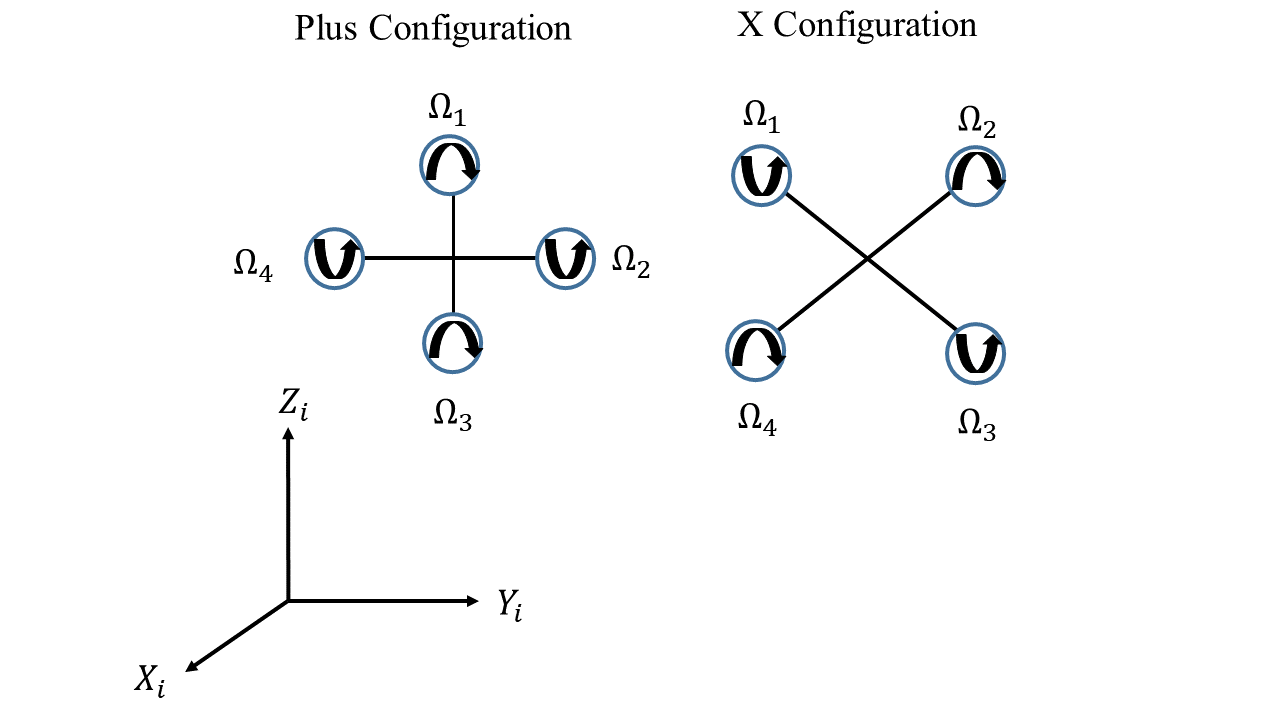
\includegraphics[width=1.0\linewidth]{figures/quad configuration.png}
    % Caption that goes to List of Figures (no citation here)
   % \caption{Types of Quad configuration, and its relative motion w.r.t propeller speed}
    % Extra caption shown only under the figure, with citation
    %\caption*{Source: \cite{wallace2016dynamics}}
   % \label{fig:Types of Quad configuration}
%\end{figure}

%\begin{figure}[h!]
   % \centering
   % \begin{minipage}{0.48\linewidth}
      %  \centering
       % 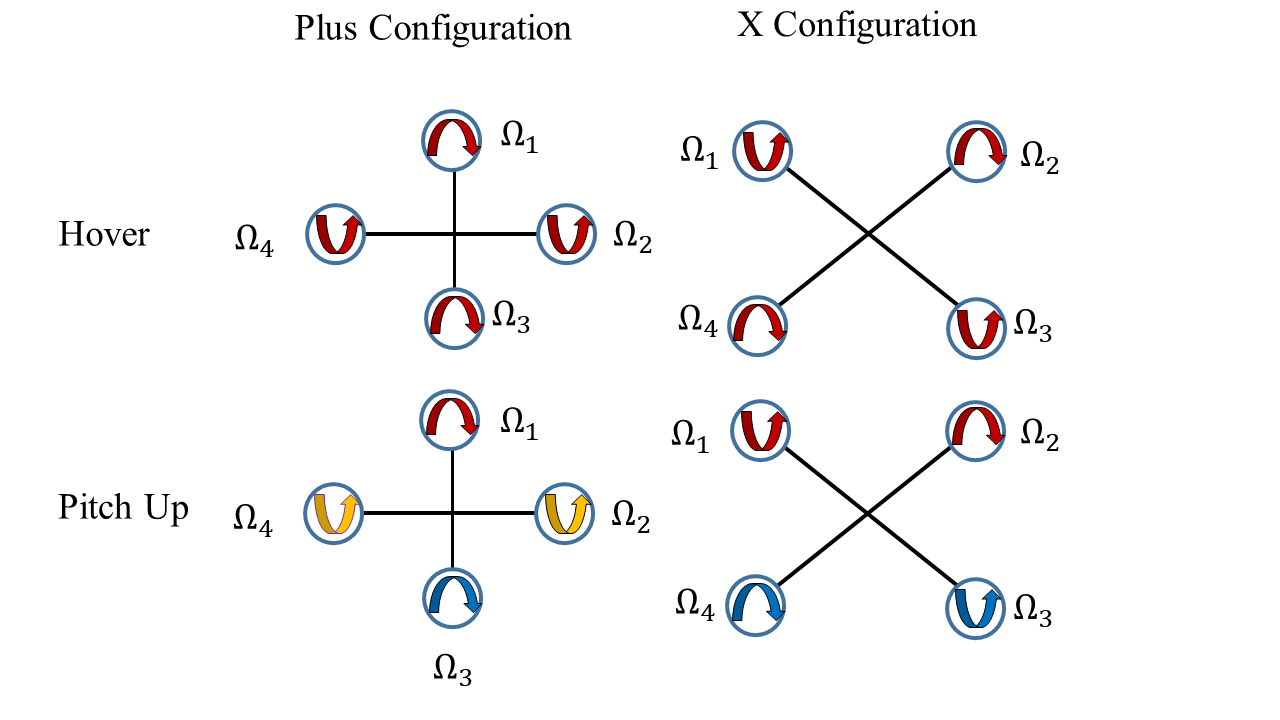
\includegraphics[width=\linewidth]{figures/quad configuration best 1.png}
       % \caption{Types of Quad configuration,  Hover and Pitch up motion with respect propeller speed}
       % \label{fig:Types of Quad configuration hover and pitch}
   % \end{minipage}
   % \hfill
   % \begin{minipage}{0.48\linewidth}
      %  \centering
       % 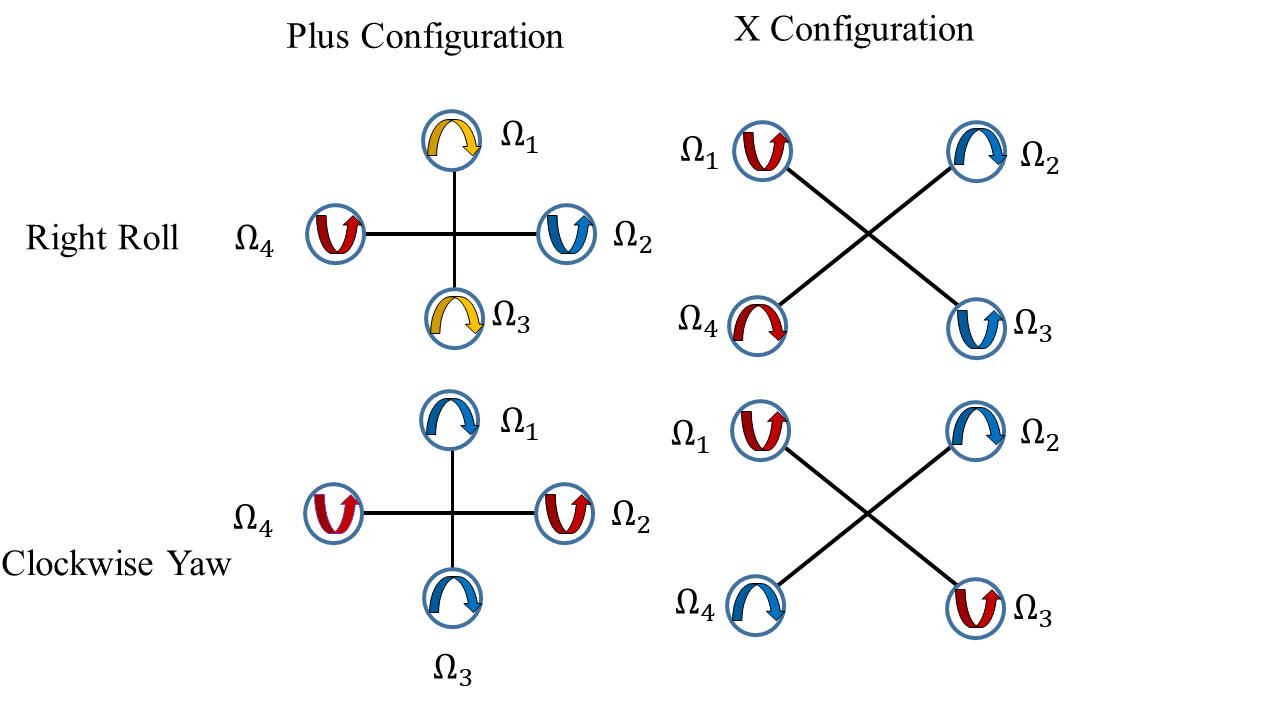
\includegraphics[width=\linewidth]{figures/quad configuration best 2nd.png}
       % \caption{Types of Quad configuration, Roll and Yaw motion with respect propeller speed}
       % \label{fig:Types of Quad configuration roll and yaw}
  %  \end{minipage}
 %\caption{Experimental quadcopter platform and test setup}
    %\label{fig:quadcopter_setup}

    
\end{figure}

\begin{figure}[h!]
    \centering
    \begin{subfigure}{0.48\linewidth}
        \centering
        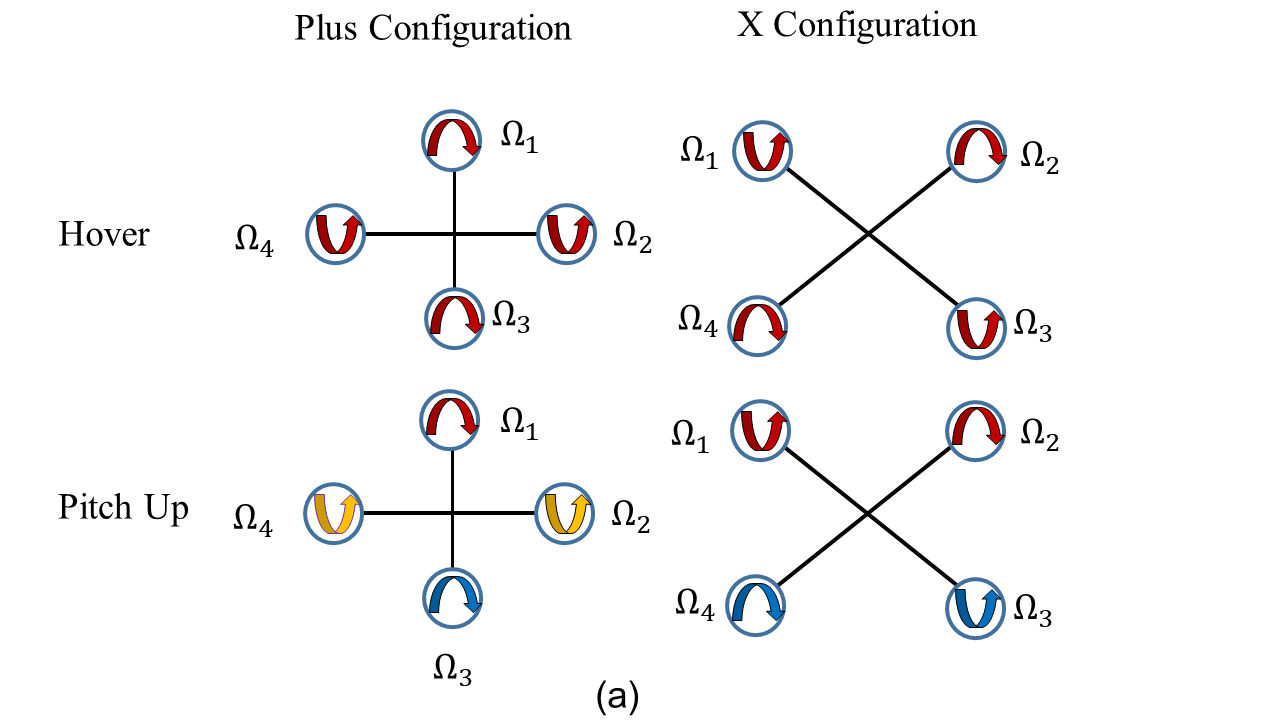
\includegraphics[width=\linewidth]{figures/quad configuration hover and pitch.png}
        \phantomcaption
        \label{fig:quad_a}
    \end{subfigure}
    \hfill
    \begin{subfigure}{0.48\linewidth}
        \centering
        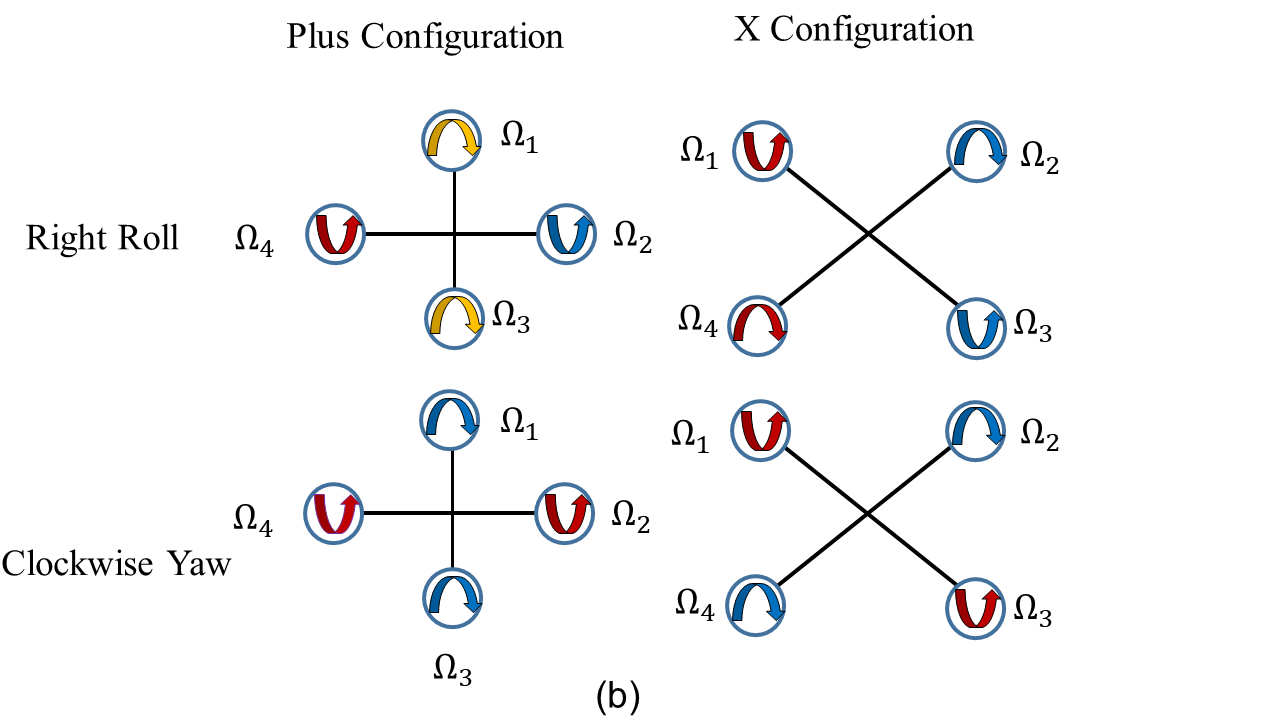
\includegraphics[width=\linewidth]{figures/quad configuration roll and yaw.png}
        \phantomcaption
        \label{fig:quad_b}
    \end{subfigure}

    \caption{Types of quadcopter configurations showing motion generation through propeller speed variation: (a) hover and pitch motion, (b) roll and yaw motion.}
    \label{fig:quad_config}
\end{figure}




Flight mode of Quadrotor can be controlled to desired pose in the space by changing the direction and velocity of each propellers\cite{alemaw2019precision}. The thrust forces caused by propellers rotation are responsible for ascending or descending flight. As shown in Figure  \ref{fig:quad_config} (b), applying speed difference between side propellers result in roll rotation coupled with y-axis translation. Similarly the pitch rotation coupled with translation motion along x-axis is caused due to the speed difference between front and rear propellers as shown in Figure  \ref{fig:quad_config} (a). The yaw rotation is caused due to unbalanced rotation speed of the four propellers. Unlike the roll and pitch rotation, yaw rotation is the result of reactive torques shown below which can be found also in Figure.\ref{fig:Quadrotor free body diagram} 

\[
\tau_i, \; i = 1,2,3,4 \text{ represents the individual torque of each rotor,}
\]
\[
\Omega_i, \; i = 1,2,3,4 \text{ represents the angular velocity of each rotor.}
\]
Increasing CCW rotated propellers speed result in yaw CW vehicle rotation.
In order to design mathematical model of Quadrotor, the coordinate frame of Quadrotor has to be defined first. There are two coordinate frames, as shown in Figure~\ref{fig:Quadrotor free body diagram}, that the Quadrotor will operate in: inertial or fixed frame $(x_i, y_i, z_i)$ and body or mobile frame $(x_b, y_b, z_b)$\cite{lv2014sliding}. Inertial Frame (IF) is where the Newton laws are valid and defined with respect to the ground with positive z axis pointing in the opposite direction of gravity, whereas Body Frame (BF) is defined with respect to Center of Gravity (CoG) of the Quadrotor with its axes  fixed to the body.
%Here we are going to use the two types of Right Hand Rule: the one in left side used to determine the positive direction of axis of rotation, and the one in right side used to determine direction of angular position where thumb pointing positive direction of axis of rotation and the turned fingers pointing positive direction of angular position.


\begin{figure}[h!]
    \centering
    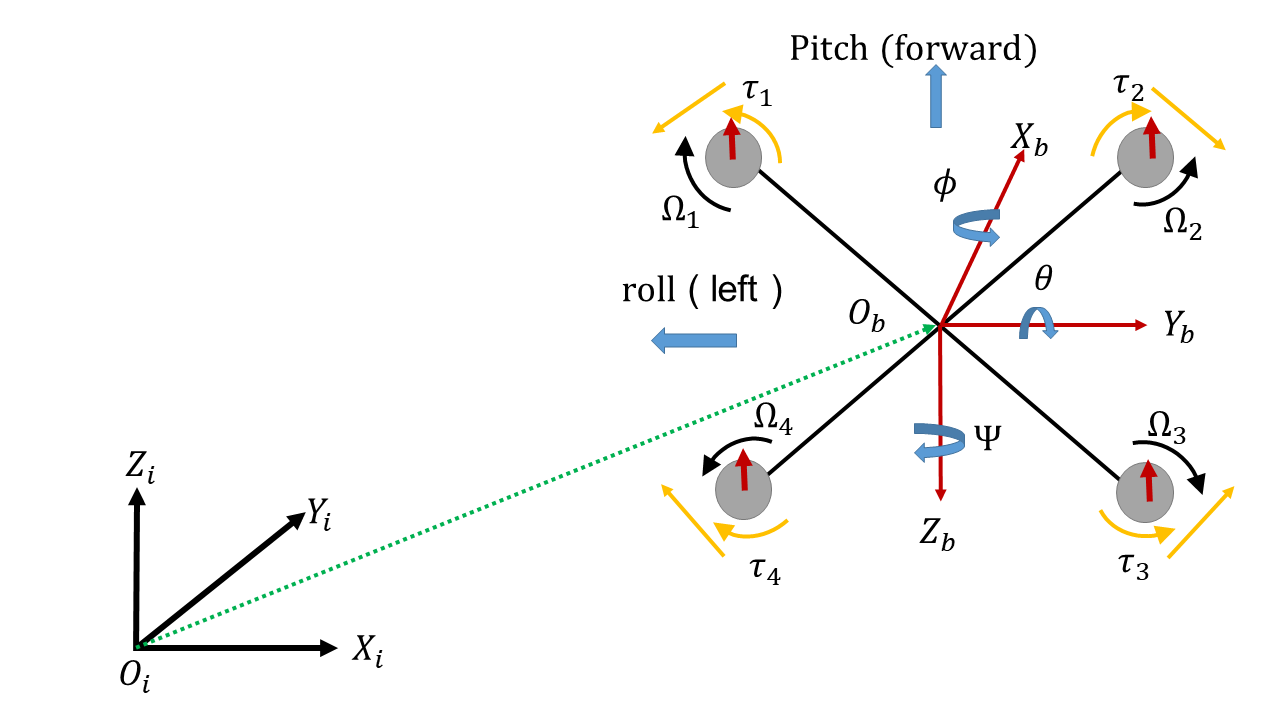
\includegraphics[width=1\linewidth]{figures/Quadcopter FBD.png}
    \caption{Quadrotor free body diagram and its reference frames }
    \label{fig:Quadrotor free body diagram}
\end{figure}





The necessity of diffining those reference frames is because of: actuator inputs $U$ and thrusts $T$, Inertial Measurement Unit (IMU), Accelerometer, Magnetometer  are manipulated and measure quantities with respect to Body Frame (BF). Also  GPS measures position with respect to Inertial Frame and Model development is carried out with respect to IF since Newton laws are valid in IF only.

%\begin{itemize}
    %\item 
    
    %\item Inertial Measurement Unit (IMU), Accelerometer, and Magnetometer measure quantities with respect to BF,
    %\item GPS measures position with respect to IF, and
    %\item Model development is carried out with respect to IF since Newton laws are valid in IF only.
%\end{itemize}

\subsection{Coordinate Frames Transformation}

%Coordinate frames transformation is used to transform quantities between the two reference frames. In this sub-section we are going to see the two most known approaches for coordinate transformation: Euler or classical approach, and Quaternion approach.
Coordinate frames transformation was used to transform quantities between the two reference frames. In this subsection  the  Quaternion approach for coordinate transformation was realized as controller designed  based on this.


%\subsubsubsection{\textbf{Euler or Classical Approach}}

%Euler approach uses three parameters: roll $\phi$, pitch $\theta$, and yaw $\psi$ to describe orientation in 3D space, and it requires three consecutive rotations along roll, pitch and yaw, to transform BF quantities into IF quantities. Since GPS measures position w.r.t IF, single axis rotational matrix can be constructed by projecting IF coordinates into BF coordinates. Projection matrix in terms of dot products of the basis vectors of the two coordinate frames is given as\textsuperscript{[24]}:

%\begin{equation}
%R^b_e =
%\begin{bmatrix}
%X_e \cdot X_b & Y_e \cdot X_b & Z_e \cdot X_b \\
%X_e \cdot Y_b & Y_e \cdot Y_b & Z_e \cdot Y_b \\
%X_e \cdot Z_b & Y_e \cdot Z_b & Z_e \cdot Z_b
%\end{bmatrix}
%\label{eq:rotation_matrix}
%\tag{3.1}
%\end{equation}



%\textit{Euler rotation theorem} states that orientation of 3D coordinate frame w.r.t another can be described by successive rotation about three axes in the way that no two successive rotations are about the same axes. Therefore; Yaw-Roll-Pitch (zyx) sequence rotation matrix, which is the most commonly used conventions from the 12 different possible rotation sequences: xyz, xzy, yxz, yzx, zyx, zxy, xyx, xzx, yyy, yzy, zyz, and zyz\cite{waldron2007handbook}, is taken to project IF quantities into Quadrotor BF quantities as shown in Figure\ref{fig:cordinate frame transformation}.
% \begin{figure}[h!]
%     \centering
%     \includegraphics[width=0.5\linewidth]{Figures/cordinate frame transformation.PNG}
%     \caption{\textit{Coordinate transformation from IF to the BF by using Euler angles} $(\phi, \theta, \psi)$}
%     \label{fig:cordinate frame transformation}
% \end{figure}

 %By using equation (3.1) we can get rotation matrix along z-axis $R_z(\psi)$ as

% \begin{equation}
% R_z(\psi) =
% \begin{bmatrix}
% c_\psi & -s_\psi & 0 \\
% s_\psi &  c_\psi & 0 \\
% 0      &  0      & 1
% \end{bmatrix}
% \tag{3.2}
% \end{equation}

% , along y-axis $R_y(\theta)$ as

% \begin{equation}
% R_y(\theta) =
% \begin{bmatrix}
% c_\theta & 0 & s_\theta \\
% 0        & 1 & 0 \\
% -s_\theta& 0 & c_\theta
% \end{bmatrix}
% \tag{3.3}
% \end{equation}

% , and along x-axis $R_x(\phi)$ as

% \begin{equation}
% R_x(\phi) =
% \begin{bmatrix}
% 1 & 0      & 0 \\
% 0 & c_\phi & -s_\phi \\
% 0 & s_\phi &  c_\phi
% \end{bmatrix}
% \tag{3.4}
% \end{equation}

% Where: $c_\theta = \cos\theta$, $s_\theta = \sin\theta$, and $T_\theta = \tan\theta$

%\textit{\textbf{3D Rotation matrix}} $R^b_e$, which transform IF translational position quantities into the BF coordinates, can be obtained by cascading the single axis rotation matrix that described in equation (3.2--3.4) with matrix multiplication as follows:


% \begin{equation}
% R^b_e = R_z(\psi) \cdot R_y(\theta) \cdot R_x(\phi)
% \tag{3.5a}
% \end{equation}

% \[
% R^b_e =
% \begin{bmatrix}
% c_\psi & -s_\psi & 0 \\
% s_\psi &  c_\psi & 0 \\
% 0      &  0      & 1
% \end{bmatrix}
% \begin{bmatrix}
% c_\theta & 0 & s_\theta \\
% 0        & 1 & 0 \\
% -s_\theta& 0 & c_\theta
% \end{bmatrix}
% \begin{bmatrix}
% 1 & 0      & 0 \\
% 0 & c_\phi & -s_\phi \\
% 0 & s_\phi &  c_\phi
% \end{bmatrix}
% \]

% \[
% \begin{equation}
% R^b_e =
% \begin{bmatrix}
% X_e \cdot X_b & Y_e \cdot X_b & Z_e \cdot X_b \\
% X_e \cdot Y_b & Y_e \cdot Y_b & Z_e \cdot Y_b \\
% X_e \cdot Z_b & Y_e \cdot Z_b & Z_e \cdot Z_b
% \end{bmatrix}
% \label{eq:rotation_matrix}
% \tag{3.1}
% \end{equation}
% \]

% Since determinant of individual rotation matrices is one, the cascade of 3D
% rotation matrices R^b_e also has determinant one, i.e., it is orthogonal.
% Therefore, (R^b_e)^T R^b_e = I, and we have (R^b_e)^T = (R^b_e)^{-1} = R^e_b.
% Thus, the 3D rotation matrix that projects body-frame (BF) quantities to the
% inertial frame (IF), R^e_b, is expressed as:
% \begin{equation}
% R^e_b =
% \begin{bmatrix}
%  c_\psi c_\theta & c_\psi s_\theta s_\phi - s_\psi c_\phi & c_\psi s_\theta c_\phi + s_\psi s_\phi \\
%  s_\psi c_\theta & s_\psi s_\theta s_\phi + c_\psi c_\phi & s_\psi s_\theta c_\phi - c_\psi s_\phi \\
% - s_\theta       & c_\theta s_\phi                        & c_\theta c_\phi
% \end{bmatrix}
% \tag{3.5}
% \end{equation}



% \textit{Transformation matrixes for angular velocities} relate Euler angle rates between IF: $[\dot{\phi}, \dot{\theta}, \dot{\psi}]^T$ and BF: $[p, q, r]^T$. To project BF rates into IF, we first rotate BF around x-axis by roll angle $\phi$, which is then followed by rotating around y-axis by pitch angle $\theta$ and finally around z-axis by yaw angle $\psi$, and these steps are expressed in Figure \ref{fig:Rotational sequence} as

%\begin{figure}[h!]
    %\centering
    %\includegraphics[width=0.5\linewidth]{Figures/Rotate transformation.PNG}
    %\caption{Rotation sequence from roll $\rightarrow$ pitch $\rightarrow$ yaw\cite{en14051232}}
    %\label{fig:Rotational sequence}
%\end{figure}

% \begin{figure}[h!]
%     \centering
%     \includegraphics[width=0.5\linewidth]{Figures/Rotate transformation.PNG}
%
%     % Caption that appears in List of Figures (NO citation here)
%     \caption{Rotation sequence from roll $\rightarrow$ pitch $\rightarrow$ yaw}
%
%     % Caption that appears ONLY under the figure (WITH citation)
%     \caption*{Source: \cite{en14051232}}
%
%     \label{fig:Rotational sequence}
% \end{figure}




% The projections of angular rates which are expressed in the vector of Euler rates in the BF into IF can be done as follows. First, we start from backwards with the last rotation $\dot{\phi}$, this is about x-axis which has the same unit vector with $p$, so no frame transformation is required i.e., trivially $\dot{\phi} = p$. Then, lets look at $\dot{\theta}$ this rotation is about y-axis which lags behind BF axis by a roll rotation, so to bring it to BF axis we need to pre-multiply by $R_x(\phi)$. Finally, $\dot{\psi}$ is about z-axis which lags behind by two rotations, so it’s pre-multiplied by $R_z(\phi)R_y(\theta)$. In the case of BF has different origin than the IF, BF rates are calculated from IF by using the following equation\cite{en14051232}:

% \begin{equation}
% \vec{X} = \vec{X}_o + R^T \vec{X}_b
% \tag{3.6a}
% \end{equation}

% Where: $\vec{X}_o$ is the location of moving origin that expressed in IF coordinates. Since IMU measure quantities w.r.t BF whereas GPS measure Euler parameters w.r.t IF, we project first, IF into BF in terms of Euler parameters. Then by inverting coefficient matrix, transformation matrix that relate BF rates with IF is obtained. To do that we maneuver from BF to IF by using inverse of a single axis rotation matrix in equation (3.2--3.4). Since rotation matrixes are orthogonal, their inverse is equal to transpose of corresponding matrix.  
%
%
%
%\[
%\begin{bmatrix}
%p \\ q \\ r
%\end{bmatrix}
%=
%\begin{bmatrix}
%\dot{\phi} \\ 0 \\ 0
%\end{bmatrix}
%+ R_x^T(\phi)
%\begin{bmatrix}
%0 \\ \dot{\theta} \\ 0
%\end{bmatrix}
%+ R_x^T(\phi) R_y^T(\theta)
%\begin{bmatrix}
%0 \\ 0 \\ \dot{\psi}
%\end{bmatrix}
%\]
%Expanding:
%
% First term
%
% \[
% =
% \begin{bmatrix}
% 1 & 0 & 0 \\
% 0 & c_\phi & s_\phi \\
% 0 & -s_\phi & c_\phi
% \end{bmatrix}
% \begin{bmatrix}
% 0 \\ \dot{\theta} \\ 0
% \end{bmatrix}
% +
% %
% % Second term
% %
% \begin{bmatrix}
% 1 & 0 & 0 \\
% 0 & c_\phi & s_\phi \\
% 0 & -s_\phi & c_\phi
% \end{bmatrix}
% \begin{bmatrix}
% c_\theta & 0 & s_\theta \\
% 0 & 1 & 0 \\
% -s_\theta & 0 & c_\theta
% \end{bmatrix}
% \begin{bmatrix}
% 0 \\ 0 \\ \dot{\psi}
% \end{bmatrix}
% + 
% %
% % Third term
% %
% \begin{bmatrix}
% \dot{\phi} \\ 0 \\ 0
% \end{bmatrix}
% \]

% Simplifying:
%
% \[
% =
% \begin{bmatrix}
% \dot{\phi} \\ c_\phi \dot{\theta} \\ -s_\phi \dot{\theta}
% \end{bmatrix}
% +
% \begin{bmatrix}
% 0 \\ s_\phi s_\theta \dot{\psi} + c_\phi \dot{\psi} \\ c_\phi s_\theta \dot{\psi} - s_\phi \dot{\psi}
% \end{bmatrix}
% \]
%
% Thus,
%
% \begin{equation}
% \begin{bmatrix}
% p \\ q \\ r
% \end{bmatrix}
% =
% \begin{bmatrix}
% 1 & 0 & -s_\theta \\
% 0 & c_\phi & s_\phi c_\theta \\
% 0 & -s_\phi & c_\phi c_\theta
% \end{bmatrix}
% \begin{bmatrix}
% \dot{\phi} \\ \dot{\theta} \\ \dot{\psi}
% \end{bmatrix}
% \tag{3.6b}
% \end{equation}

% However, to drive Quadrotor model we need velocity on IF. So, by inverting the above coefficient matrix, rate transformation matrixes that project BF rates into IF becomes
%
% \begin{equation}
% \begin{bmatrix}
% \dot{\phi} \\
% \dot{\theta} \\
% \dot{\psi}
% \end{bmatrix}
% =
% \begin{bmatrix}
% 1 & s_\phi T_\theta & c_\phi T_\theta \\
% 0 & c_\phi          & -s_\phi \\
% 0 & \tfrac{s_\phi}{c_\theta} & \tfrac{c_\phi}{c_\theta}
% \end{bmatrix}
% \begin{bmatrix}
% p \\ q \\ r
% \end{bmatrix}
% \tag{3.6}
% \end{equation}

\subsection*{\textbf{Quaternion Approach}}

%The idea of Quaternions was first proposed by W.R Hamilton in 1843 \cite{hamilton1866elements} as an extension of the imaginary part of complex numbers. He first realized that complex numbers are a powerful tool to manage rotation in 2-dimensional space, then he supposed that a generalization of the complex numbers would also result in a good tool to manage rotations in 3-dimensional space. This makes quaternion as a hyper complex number with four dimensions, one of which is real while the other three are imaginary, that can be utilized to avoid the nonlinearity, geometric singularity, and computational cost usually associated with the Euler angles\cite{fresk2013full,fresk2013modeling}.


The concept of quaternions was originally introduced by W.R. Hamilton in 1843 \cite{hamilton1866elements} as an extension of complex numbers to higher dimensions. Hamilton recognized that complex numbers provide an elegant framework for representing rotations in two-dimensional space and hypothesized that a generalization to higher dimensions would similarly facilitate rotation operations in three-dimensional space. Consequently, quaternions emerge as hypercomplex numbers comprising four dimensions one real component and three imaginary components which effectively circumvent the nonlinearity, geometric singularities, and computational complexity typically associated with Euler angle representations \cite{fresk2013full,fresk2013modeling}.

%Quaternion contains a scalar part $q_0$, and a three dimensional vector part: $\vec{q} = [q_1, q_2, q_3]$ with orthonormal base $[i, j, k]$  representing $[x, y, z]$ axis that satisfies the following fundamental rules introduced by W.R Hamilton \cite{hamilton1866elements}
%\begin{equation}
%q = (q_0, \vec{q}) = \left( \cos\frac{\theta}{2}, \; \sin\frac{\theta}{2} \, \hat{u} \right)
%\tag{3.1}
%\label{eqn 3.1}
%\end{equation}

%\[
%ij = k = -ji,\quad jk = i = -kj,\quad ki = j = -ik.
%\]

%Hence, \[
%i^2 = j^2 = k^2 = ijk = -1
%\]
%Also there are three common conventions for representing a quaternion:
%\[
%q = q_0 + q_1 \hat{i} + q_2 \hat{j} + q_3 \hat{k}
%= [q_0, q_1, q_2, q_3] = (q_0, \vec{q})
%\]
%%%%%%%%%%%%%%%%%%%%%%%%%%%%%%%%%%%
A quaternion consists of a scalar part $q_0$ and a three-dimensional vector part $\vec{q} = [q_1, q_2, q_3]$, which can be expressed in the form:
\begin{equation}
q = (q_0, \vec{q}) = \left( \cos\frac{\theta}{2}, \sin\frac{\theta}{2} \, \hat{u} \right),
\label{eqn:quaternion_form}
\end{equation}
where $\theta$ represents the rotation angle and $\hat{u}$ is the unit vector along the rotation axis.The vector part is defined with respect to an orthonormal basis $[\hat{i}, \hat{j}, \hat{k}]$ representing the $[x, y, z]$ coordinate axes, respectively. These basis elements satisfy the fundamental multiplication rules introduced by W.R. Hamilton \cite{hamilton1866elements}:
\begin{equation}
ij = k = -ji, \quad jk = i = -kj, \quad ki = j = -ik.
\label{eqn:hamilton_rules}
\end{equation}

From these rules, it follows that:
\begin{equation}
i^2 = j^2 = k^2 = ijk = -1.
\label{eqn:quaternion_squares}
\end{equation}

There are three equivalent conventions commonly used for representing a quaternion:
\begin{equation}
q = q_0 + q_1 \hat{i} + q_2 \hat{j} + q_3 \hat{k} = [q_0, q_1, q_2, q_3] = (q_0, \vec{q}).
\label{eqn:quaternion_representations}
\end{equation}


%%%%%%%%%%%%%%%%%%%%%%%%%%%%%

%In order to represent a valid 3D orientation or to compute valid vector rotations, the quaternion must be normalized. The normalized quaternion is ideally suitable for representing orientation of an object in 3D space and transforming orientation of coordinates between any two reference frames. Quaternion normalization can be done just like a four dimension vector by dividing each of four components by its Euclidean norm, and it’s mathematically expressed as.

%\[
%q = \frac{q_0 + q_1 i + q_2 j + q_3 k}{\sqrt{q_0^2 + q_1^2 + q_2^2 + q_3^2}},
%\]

%Where this normalized quaternion physically interpreted as an angle in 3D space about which a single rotation defines the final orientation of a frame relative to some initial reference frame i.e., it represent orientation by a single rotation around an axis $\hat{u}$ as shown in figure \ref{fig:Quaternion representation of rotation along rotation axis}. In case of Euler rotation theorem, this requires three consecutive rotations about a single axis along yaw, pitch and roll directions.

%%%%%%%%%%%%%%%%%%%%%
For valid representation of 3D orientations and vector rotations, quaternions must be normalized. Normalized quaternions provide an optimal framework for describing object orientations in three-dimensional space and transforming coordinates between reference frames. Normalization follows the standard procedure for four-dimensional vectors, dividing each component by the quaternion's Euclidean norm:
\begin{equation}
%q_{\text{norm}} = \frac{q_0 + q_1 \hat{i} + q_2 \hat{j} + q_3 \hat{k}}{\sqrt{q_0^2 + q_1^2 + q_2^2 + q_3^2}}.
q = \frac{q_0 + q_1 \hat{i} + q_2 \hat{j} + q_3 \hat{k}}{\sqrt{q_0^2 + q_1^2 + q_2^2 + q_3^2}}.
\label{eqn:quaternion_normalization}
\end{equation}

The normalized quaternion physically represents a single rotation about an axis $\hat{u}$ in 3D space, defining the orientation of a frame relative to a reference frame as shown in Figure~\ref{fig:Quaternion representation of rotation along rotation axis}). This contrasts with Euler's rotation theorem, which requires three consecutive rotations about individual axes (yaw, pitch, and roll).


%%%%%%%%%%%%%%%%




\begin{figure}[h!]
    \centering
    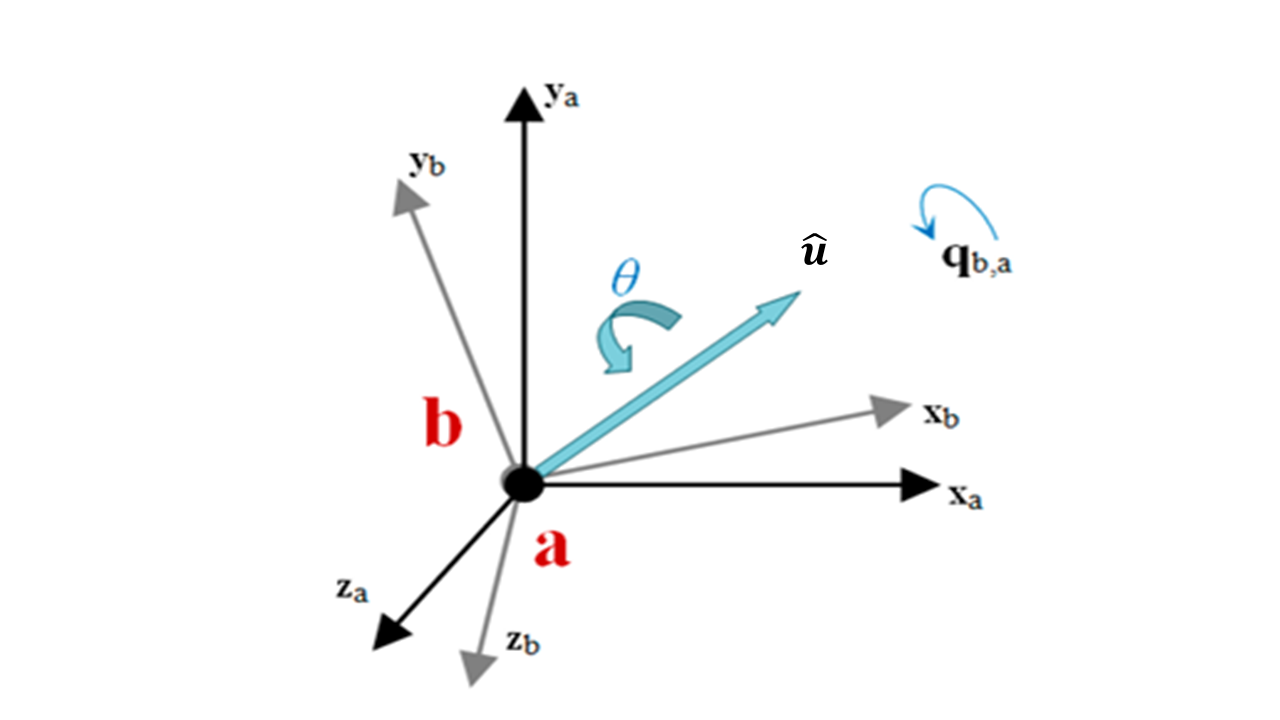
\includegraphics[width=0.5\linewidth]{figures/quad rotation.png}
    \caption{Quaternion representation of rotation along rotation axis $\hat{u}$}
    \label{fig:Quaternion representation of rotation along rotation axis}
\end{figure}
%Since normalized or unit quaternion provides a convenient mathematical notation for representing orientations and rotations of objects in 3D space, the  unit quaternion notion was used to derive Quadrotor model. In unit quaternion, scalar component gives the rotation angle whereas the vector part gives the direction of the rotation axis as shown in Eq.\ref{eqn:quaternion_form}.

%\begin{equation}
%q = (q_0, \vec{q}) = \left( \cos\frac{\theta}{2}, \; \sin\frac{\theta}{2} \, \hat{u} \right)
%\tag{3.1}
%\label{eqn 3.1}
%\end{equation}

%where $\hat{u}$ is a unit vector which is constant, not changing with rotation, and it is formed as 
%\[
%\hat{u} = \frac{\vec{q}}{||\vec{q}||}.
%\]

%Quaternion has its own special set of mathematical operator called \textbf{quaternion product} ‘$\otimes$’, which is extensively used in vector transformation and rotational kinematics. The product between two quaternion $q_a = (q_{0a}, \vec{q}_a)$ and $q_b = (q_{0b}, \vec{q}_b)$, is manipulated as
%\begin{equation}
%q_a \otimes q_b = (q_{0a}, \vec{q}_a) \otimes (q_{0b}, \vec{q}_b) = (q_{0a}q_{0b} - \vec{q}_a \cdot \vec{q}_b, \; q_{0a}\vec{q}_b + q_{0b}\vec{q}_a + \vec{q}_a \times \vec{q}_b)
%\tag{3.2}
%\label{eqn 3.2}
%\end{equation}

%Coordinate transformation between any two different reference frames by using quaternion rotation is computed as\cite{guerrero2017quadrotor}:

%\begin{equation}
%X = q \otimes X' \otimes q^*,
%\tag{3.3a}
%\label{{3.3a}}
%\end{equation}

%where $X$ is the rotated vector and  $X'$ denotes vector to be rotated. Since $q$ is unit norm Quaternion i.e. $||q|| = 1$, its inverse is equal to its conjugate. This is proved as.

%\[
%q^{-1} = \frac{1}{q} = \frac{1}{q} \cdot \frac{q^*}{q^*} = \frac{q^*}{||q||^2} = \frac{q^*}{1^2} = q^*.
%\]

%Hence,

%\begin{equation}
%X = q \otimes X' \otimes q^*
%\tag{3.3b}
%\label{3.3b}
%\end{equation}

%%%%%%%%%%%%%%%%%%%%%%%%%%%%%%%%%%%%%%%
Given their elegant mathematical properties, unit quaternions are employed to derive the quadrotor dynamic model. In the unit quaternion representation shown in Equation~\ref{eqn:quaternion_form}, the scalar component $q_0 = \cos(\theta/2)$ encodes the rotation angle, while the vector component $\vec{q} = \sin(\theta/2)\hat{u}$ specifies the rotation axis direction, where $\hat{u}$ is the unit vector:
\begin{equation}
\hat{u} = \frac{\vec{q}}{\|\vec{q}\|}.
\label{eqn:rotation_axis}
\end{equation}

Quaternions utilize a specialized multiplication operator called the \textbf{quaternion product}, denoted by `$\otimes$', which is fundamental to vector transformations and rotational kinematics. For two quaternions $q_a = (q_{0a}, \vec{q}_a)$ and $q_b = (q_{0b}, \vec{q}_b)$, the product is defined as:
\begin{equation}
q_a \otimes q_b = \left( q_{0a}q_{0b} - \vec{q}_a \cdot \vec{q}_b, \; q_{0a}\vec{q}_b + q_{0b}\vec{q}_a + \vec{q}_a \times \vec{q}_b \right).
\label{eqn:quaternion_product}
\end{equation}

Coordinate transformations between reference frames are performed using quaternion rotation \cite{guerrero2017quadrotor}:
\begin{equation}
X = q \otimes X' \otimes q^*,
\label{eqn:quaternion_rotation}
\end{equation}
where $X'$ is the vector in the original frame, $X$ is the transformed vector, and $q^*$ denotes the quaternion conjugate. For unit quaternions ($\|q\| = 1$), the inverse equals the conjugate, since:
\begin{equation}
q^{-1} = \frac{q^*}{\|q\|^2} = \frac{q^*}{1} = q^*.
\label{eqn:quaternion_inverse}
\end{equation}


%%%%%%%%%%%%%%%%%%%%%%%%%%%%%%%%%%%%%%%%%%%%

%This implies, multiplying two or more rotation quaternion produces another rotation quaternion that represents the total rotation obtained by performing each individual rotation for each quaternion. Vectors can be transformed from one axis system to another if they are first transformed into quaternion with a zero scalar value, also this is known as pure quaternion. This is used to transform the vector coordinate between different rotated reference frames. Since quaternion measures quantities with respect to  IF, quaternion based Rotation matrix that transform quantities from IF to the BF is obtained as.
%\[
%\begin{bmatrix} 0 \\ r_b \end{bmatrix} 
%= q \otimes \begin{bmatrix} 0 \\ r_i \end{bmatrix} \otimes q^*
%\]

%\[
%q \otimes \begin{bmatrix} 0 \\ r_i \end{bmatrix} = [q_0, q_1, q_2, q_3] \otimes [0, x_i, y_i, z_i]
%\]

%\noindent where
%\begin{itemize}
   % \item $q$ : unit quaternion representing orientation
   % \item $q_0$ : scalar part of the quaternion given in Eq. \ref{eqn 3.1}
   % \item $q_1, q_2, q_3$ : vector part of the quaternion given in Eq. \ref{eqn 3.1}
%\end{itemize}

%Let $v_1 = [q_1, q_2, q_3]$, and $v_2 = [x_i, y_i, z_i]$ then by using equation \ref{eqn 3.2} it was found  

%\[
%[q_0, v_1] \otimes [0, v_2] = (q_0 \cdot 0 - v_1 \cdot v_2, \; q_0 v_2 + 0 \cdot v_1 + v_1 \times v_2)
%\]

%\[
%\Rightarrow v_1 \cdot v_2 = [q_1, q_2, q_3] \cdot [x_i, y_i, z_i] = q_1 x_i + q_2 y_i + q_3 z_i
%\]

%\[
%\Rightarrow v_1 \times v_2 = 
%\begin{bmatrix}
%q_1 \\ q_2 \\ q_3
%\end{bmatrix}
%\times
%\begin{bmatrix}
%x_i \\ y_i \\ z_i
%\end{bmatrix}
%=
%\begin{bmatrix}
%q_2 z_i - q_3 y_i \\
%q_3 x_i - q_1 z_i \\
%q_1 y_i - q_2 x_i
%\end{bmatrix}
%\]

%Let $w = (w_0, \vec{w}) = q \otimes \begin{bmatrix} 0 \\ r_i \end{bmatrix}$, where $w_0$ is scalar part and $\vec{w}$ is vector part of Quaternion $w$.

%\[
%w =
%\begin{bmatrix}
%q_0 \cdot 0 - v_1 \cdot v_2 \\
%q_0 v_2 + 0 \cdot v_1 + v_1 \times v_2
%\end{bmatrix}
%=
%\begin{bmatrix}
%-(q_1 x_i + q_2 y_i + q_3 z_i) \\
%q_0 x_i + q_2 z_i - q_3 y_i \\
%q_0 y_i + q_3 x_i - q_1 z_i \\
%q_0 z_i + q_1 y_i - q_2 x_i
%\end{bmatrix}
%\]

%Then, the total rotation is solved by multiplying $w$ with $q^*$:

%\[
%q \otimes \begin{bmatrix} 0 \\ r_i \end{bmatrix} \otimes q^* = w \otimes q^*
%\]

%where $q^* = (q_0, -q_1, -q_2, -q_3) = (q_0, -\vec{q})$.

%By using equation \ref{eqn 3.2}, the two quaternion product is solved as follows:


%%%%%%%%%%%%%%%%%%%%%%%%%%


An important property of quaternions is that the product of two or more rotation quaternions yields another rotation quaternion representing the cumulative effect of applying each individual rotation sequentially. This compositional property makes quaternions particularly efficient for representing complex orientation sequences.To transform vectors between reference frames, they are first expressed as pure quaternions quaternions with zero scalar components. A vector $\bm{r}_i = [x_i, y_i, z_i]^T$ in the inertial frame (IF) is represented as the pure quaternion $(0, \bm{r}_i)$. The transformation to the body frame (BF) is then computed as:
\begin{equation}
\begin{bmatrix} 0 \\ \bm{r}_b \end{bmatrix} 
= q \otimes \begin{bmatrix} 0 \\ \bm{r}_i \end{bmatrix} \otimes q^*,
\label{eqn:quaternion_frame_transform}
\end{equation}
where $q = (q_0, q_1, q_2, q_3)$ is the unit quaternion representing the body orientation relative to the inertial frame, and $q^* = (q_0, -q_1, -q_2, -q_3)$ denotes its conjugate.

%\subsubsection*{Derivation of the Transformation}

The transformation is evaluated through two successive quaternion multiplications.

\paragraph{First multiplication: $w = q \otimes \begin{bmatrix} 0 \\ \bm{r}_i \end{bmatrix}$}

Define the vector components $\bm{v}_1 = [q_1, q_2, q_3]^T$ and $\bm{v}_2 = [x_i, y_i, z_i]^T$. Applying the quaternion product formula (Equation~\ref{eqn:quaternion_product}):
\begin{equation}
(q_0, \bm{v}_1) \otimes (0, \bm{v}_2) = (q_0 \cdot 0 - \bm{v}_1 \cdot \bm{v}_2, \; q_0\bm{v}_2 + 0 \cdot \bm{v}_1 + \bm{v}_1 \times \bm{v}_2),
\end{equation}
which simplifies to:
\begin{equation}
w = (-\bm{v}_1 \cdot \bm{v}_2, \; q_0\bm{v}_2 + \bm{v}_1 \times \bm{v}_2).
\end{equation}

The required dot and cross products are:
\begin{align}
\bm{v}_1 \cdot \bm{v}_2 &= q_1 x_i + q_2 y_i + q_3 z_i, \\
\bm{v}_1 \times \bm{v}_2 &= 
\begin{bmatrix}
q_2 z_i - q_3 y_i \\
q_3 x_i - q_1 z_i \\
q_1 y_i - q_2 x_i
\end{bmatrix}.
\end{align}

Substituting these yields the intermediate quaternion $w = (w_0, \bm{w})$:
\begin{equation}
w = 
\begin{bmatrix}
-(q_1 x_i + q_2 y_i + q_3 z_i) \\
q_0 x_i + q_2 z_i - q_3 y_i \\
q_0 y_i + q_3 x_i - q_1 z_i \\
q_0 z_i + q_1 y_i - q_2 x_i
\end{bmatrix}.
\label{eqn:intermediate_w}
\end{equation}

\paragraph{Second multiplication: $\bm{r}_b^q = w \otimes q^*$}

The final transformation is obtained by multiplying the intermediate quaternion $w$ with the conjugate $q^* = (q_0, -q_1, -q_2, -q_3)$:
\begin{equation}
\begin{bmatrix} 0 \\ \bm{r}_b \end{bmatrix} = w \otimes q^*.
\label{eqn:final_step}
\end{equation}

This second quaternion product, evaluated using Equation~\ref{eqn:quaternion_product}, yields the rotated vector $\bm{r}_b$ in the body frame. The scalar component of the result is zero, confirming that the output is a pure quaternion representing the transformed vector.

%%%%%%%%%%%%%%%%%%%%%%%%%%%%%


%\begin{small}
%\begin{align*}
%w \otimes q^* &= (w_0 q_0 - \vec{w}\cdot \vec{q},\; w_0 \vec{q} + q_0 \vec{w} + \vec{w} \times \vec{q}) \\[1ex]
%\Rightarrow w_0 q_0 &= (-q_1 x_i - q_2 y_i - q_3 z_i) q_0 
%= -q_0 q_1 x_i - q_0 q_2 y_i - q_0 q_3 z_i \\[1ex]
%\Rightarrow \vec{w}\cdot \vec{q} &= (q_0 x_i + q_2 z_i - q_3 y_i,\; 
%q_0 y_i + q_3 x_i - q_1 z_i,\; 
%q_0 z_i + q_1 y_i - q_2 x_i) \cdot (-q_1,-q_2,-q_3) \\[1ex]
%&= -q_0 q_1 x_i - q_0 q_2 y_i - q_0 q_3 z_i
%\end{align*}
%\end{small}

%Hence, the real part becomes  
%\[
%w_0 q_0 - \vec{w}\cdot \vec{q} = -q_0 q_1 x_i - q_0 q_2 y_i - q_0 q_3 z_i + q_0 q_1 x_i + q_0 q_2 y_i + q_0 q_3 z_i = 0
%\]

%\noindent$\bullet \; w_0 \vec{q}$:
%\[
%(-q_1 x_i - q_2 y_i - q_3 z_i)(-q_1,-q_2,-q_3) =
%\begin{bmatrix}
%q_1^2 x_i + q_1 q_2 y_i + q_1 q_3 z_i \\
%q_2 q_1 x_i + q_2^2 y_i + q_2 q_3 z_i \\
%q_3 q_1 x_i + q_3 q_2 y_i + q_3^2 z_i
%\end{bmatrix}
%\]

%\noindent$\bullet \; q_0 \vec{w}$:
%\[
%q_0 \begin{bmatrix}
%q_0 x_i + q_2 z_i - q_3 y_i \\
%q_0 y_i + q_3 x_i - q_1 z_i \\
%q_0 z_i + q_1 y_i - q_2 x_i
%\end{bmatrix}
%=
%\begin{bmatrix}
%q_0^2 x_i + q_0 q_2 z_i - q_0 q_3 y_i \\
%q_0^2 y_i + q_0 q_3 x_i - q_0 q_1 z_i \\
%q_0^2 z_i + q_0 q_1 y_i - q_0 q_2 x_i
%\end{bmatrix}
%\]

%\noindent$\bullet \; \vec{w} \times \vec{q}$:
%{\small
%\[
%\begin{bmatrix}
%q_0 x_i + q_2 z_i - q_3 y_i \\
%q_0 y_i + q_3 x_i - q_1 z_i \\
%q_0 z_i + q_1 y_i - q_2 x_i
%\end{bmatrix}
%\times
%\begin{bmatrix}
%-q_1 \\ -q_2 \\ -q_3
%\end{bmatrix}
%=
%\begin{bmatrix}
%- q_0 q_3 y_i - q_3^2 x_i + q_1 q_3 z_i + q_0 q_2 z_i + q_1 q_2 y_i + q_2^2 x_i \\
%- q_0 q_1 x_i - q_1^2 y_i + q_1 q_2 x_i + q_2 q_3 z_i + q_1 q_3 x_i + q_3^2 y_i \\
%- q_0 q_2 x_i - q_2^2 z_i + q_2 q_3 y_i + q_1 q_2 z_i + q_3 q_1 x_i + q_3^2 z_i
%\end{bmatrix}
%\]
%}

%Then, by combining the bullet equations, we get the vector part of rotation matrix as:

%\begin{align*}
%w \otimes q^* &= 
%\begin{bmatrix}
%q_1^2 x_i + q_1 q_2 y_i + q_1 q_3 z_i \\
%q_1 q_2 x_i + q_2^2 y_i + q_2 q_3 z_i \\
%q_1 q_3 x_i + q_2 q_3 y_i + q_3^2 z_i
%\end{bmatrix}
%+
%\begin{bmatrix}
%q_0^2 x_i + q_0 q_2 z_i - q_0 q_3 y_i \\
%q_0^2 y_i + q_0 q_3 x_i - q_0 q_1 z_i \\
%q_0^2 z_i + q_0 q_1 y_i - q_0 q_2 x_i
%\end{bmatrix} \\[2ex]
%&\quad +
%\begin{bmatrix}
%- q_0 q_3 y_i - q_3^2 x_i + q_1 q_3 z_i + q_0 q_2 z_i + q_1 q_2 y_i + q_2^2 x_i \\
%- q_0 q_1 x_i - q_1^2 y_i + q_1 q_2 x_i + q_2 q_3 z_i + q_1 q_3 x_i + q_3^2 y_i \\
%- q_0 q_2 x_i - q_2^2 z_i + q_2 q_3 y_i + q_1 q_2 z_i + q_3 q_1 x_i + q_3^2 z_i
%\end{bmatrix} \\[2ex]
%&=
%\begin{bmatrix}
%q_1^2 x_i + 2 q_1 q_2 y_i + 2 q_1 q_3 z_i + q_0^2 x_i + 2 q_0 q_2 z_i - 2 q_0 q_3 y_i - q_3^2 x_i - q_2^2 x_i \\
%2 q_1 q_2 x_i + q_2^2 y_i + 2 q_2 q_3 z_i + q_0^2 y_i + 2 q_0 q_3 x_i - 2 q_0 q_1 z_i - q_1^2 y_i - q_3^2 y_i \\
%2 q_1 q_3 x_i + 2 q_2 q_3 y_i + q_3^2 z_i + q_0^2 z_i + 2 q_0 q_1 y_i - 2 q_0 q_2 x_i - q_1^2 z_i - q_2^2 z_i
%\end{bmatrix} \\[2ex]
%&=
%\begin{bmatrix}
%(q_0^2 + q_1^2 - q_2^2 - q_3^2)x_i + 2(q_1 q_2 - q_0 q_3) y_i + 2(q_1 q_3 + q_0 q_2) z_i \\
%2(q_1 q_2 + q_0 q_3)x_i + (q_0^2 - q_1^2 + q_2^2 - q_3^2) y_i + 2(q_2 q_3 - q_0 q_1) z_i \\
%2(q_1 q_3 - q_0 q_2)x_i + 2(q_2 q_3 + q_0 q_1) y_i + (q_0^2 - q_1^2 - q_2^2 + q_3^2) z_i
%\end{bmatrix} \\[2ex]
%&=
%\begin{bmatrix}
%q_0^2 + q_1^2 - q_2^2 - q_3^2 & 2(q_1 q_2 - q_0 q_3) & 2(q_1 q_3 + q_0 q_2) \\
%2(q_1 q_2 + q_0 q_3) & q_0^2 - q_1^2 + q_2^2 - q_3^2 & 2(q_2 q_3 - q_0 q_1) \\
%2(q_1 q_3 - q_0 q_2) & 2(q_2 q_3 + q_0 q_1) & q_0^2 - q_1^2 - q_2^2 + q_3^2
%\end{bmatrix}
%\begin{bmatrix}
%x_i \\ y_i \\ z_i
%\end{bmatrix}
%\end{align*}

%Since we are using unit quaternion to represent the attitude of a Quadrotor, they have the property of unit norm, i.e. 
%\[
%||q||^2 = q_0^2 + q_1^2 + q_2^2 + q_3^2 = 1.
%\]

%So, by utilizing this property we can simplify the above rotation matrix further.Quaternion based rotation matrix which projects IF into BF is expressed in simplified form as:
%\[
%\begin{bmatrix}
%x_b\\ y_b\\ z_b
%\end{bmatrix}
%=
%\begin{bmatrix}
%2(q_0^2+q_1^2)-1 & 2(q_1q_2-q_0q_3) & 2(q_0q_2+q_1q_3)\\
%2(q_1q_2+q_0q_3) & 2(q_0^2+q_2^2)-1 & 2(q_2q_3-q_0q_1)\\
%2(q_1q_3-q_0q_2) & 2(q_2q_3+q_0q_1) & 2(q_0^2+q_3^2)-1
%\end{bmatrix}
%\begin{bmatrix}
%x_i\\ y_i\\ z_i
%\end{bmatrix}
%\]
%%%%%%%%%%%%%%%%%%%%%%%%%%%%
%\subsection*{Derivation of Quaternion Rotation Matrix}

To complete the transformation $\bm{r}_b^q = w \otimes q^*$, we apply the quaternion product formula to $w = (w_0, \bm{w})$ and $q^* = (q_0, -\bm{q})$:
\begin{equation}
w \otimes q^* = (w_0 q_0 - \bm{w} \cdot \bm{q}, \; w_0\bm{q} + q_0\bm{w} + \bm{w} \times \bm{q}),
\label{eqn:final_product}
\end{equation}
where $\bm{q} = [q_1, q_2, q_3]^T$.

%\subsubsection*{Scalar Component (verifies pure quaternion)}

Using $w_0 = -(q_1 x_i + q_2 y_i + q_3 z_i)$ and $\bm{w} = [q_0 x_i + q_2 z_i - q_3 y_i, \; q_0 y_i + q_3 x_i - q_1 z_i, \; q_0 z_i + q_1 y_i - q_2 x_i]^T$:
\begin{align}
w_0 q_0 &= -q_0(q_1 x_i + q_2 y_i + q_3 z_i), \\
\bm{w} \cdot (-\bm{q}) &= -(q_0 x_i + q_2 z_i - q_3 y_i)(-q_1) - (q_0 y_i + q_3 x_i - q_1 z_i)(-q_2) \nonumber \\
&\quad - (q_0 z_i + q_1 y_i - q_2 x_i)(-q_3) \nonumber \\
&= q_0(q_1 x_i + q_2 y_i + q_3 z_i).
\end{align}

Therefore, the scalar part vanishes,confirming the result is a pure quaternion:
\begin{equation}
w_0 q_0 - \bm{w} \cdot \bm{q} = 0,
\end{equation}


%\subsubsection*{Vector Component}

The vector part comprises three terms: $w_0(-\bm{q}) + q_0\bm{w} + \bm{w} \times (-\bm{q})$.

\paragraph{Term 1: $w_0(-\bm{q})$}
\begin{equation}
w_0(-\bm{q}) = -(q_1 x_i + q_2 y_i + q_3 z_i)
\begin{bmatrix}
-q_1 \\ -q_2 \\ -q_3
\end{bmatrix}
=
\begin{bmatrix}
q_1^2 x_i + q_1 q_2 y_i + q_1 q_3 z_i \\
q_1 q_2 x_i + q_2^2 y_i + q_2 q_3 z_i \\
q_1 q_3 x_i + q_2 q_3 y_i + q_3^2 z_i
\end{bmatrix}.
\end{equation}

\paragraph{Term 2: $q_0\bm{w}$}
\begin{equation}
q_0\bm{w} = q_0
\begin{bmatrix}
q_0 x_i + q_2 z_i - q_3 y_i \\
q_0 y_i + q_3 x_i - q_1 z_i \\
q_0 z_i + q_1 y_i - q_2 x_i
\end{bmatrix}
=
\begin{bmatrix}
q_0^2 x_i + q_0 q_2 z_i - q_0 q_3 y_i \\
q_0^2 y_i + q_0 q_3 x_i - q_0 q_1 z_i \\
q_0^2 z_i + q_0 q_1 y_i - q_0 q_2 x_i
\end{bmatrix}.
\end{equation}

\paragraph{Term 3: $\bm{w} \times (-\bm{q})$}
\begin{equation}
\bm{w} \times (-\bm{q}) =
\begin{bmatrix}
q_0 x_i + q_2 z_i - q_3 y_i \\
q_0 y_i + q_3 x_i - q_1 z_i \\
q_0 z_i + q_1 y_i - q_2 x_i
\end{bmatrix}
\times
\begin{bmatrix}
-q_1 \\ -q_2 \\ -q_3
\end{bmatrix}
=
\begin{bmatrix}
q_2^2 x_i + q_1 q_2 y_i + q_1 q_3 z_i - q_3^2 x_i + q_0 q_2 z_i - q_0 q_3 y_i \\
q_1 q_2 x_i + q_3^2 y_i + q_2 q_3 z_i - q_1^2 y_i + q_1 q_3 x_i - q_0 q_1 z_i \\
q_1 q_3 x_i + q_2 q_3 y_i + q_3^2 z_i - q_2^2 z_i + q_0 q_1 y_i - q_0 q_2 x_i
\end{bmatrix}.
\end{equation}

%\subsubsection*{Combined Vector Part}

Summing the three terms and collecting coefficients of $x_i$, $y_i$, and $z_i$:
\begin{equation}
\bm{r}_b = 
\begin{bmatrix}
(q_0^2 + q_1^2 - q_2^2 - q_3^2)x_i + 2(q_1 q_2 - q_0 q_3)y_i + 2(q_1 q_3 + q_0 q_2)z_i \\
2(q_1 q_2 + q_0 q_3)x_i + (q_0^2 - q_1^2 + q_2^2 - q_3^2)y_i + 2(q_2 q_3 - q_0 q_1)z_i \\
2(q_1 q_3 - q_0 q_2)x_i + 2(q_2 q_3 + q_0 q_1)y_i + (q_0^2 - q_1^2 - q_2^2 + q_3^2)z_i
\end{bmatrix}.
\end{equation}

This can be expressed in matrix form as:
\begin{equation}
\bm{r}_b = R_q^{i \to b} \bm{r}_i,
\label{eqn:rotation_matrix_form}
\end{equation}
where:
\begin{equation}
R_q^{i \to b} =
\begin{bmatrix}
q_0^2 + q_1^2 - q_2^2 - q_3^2 & 2(q_1 q_2 - q_0 q_3) & 2(q_1 q_3 + q_0 q_2) \\
2(q_1 q_2 + q_0 q_3) & q_0^2 - q_1^2 + q_2^2 - q_3^2 & 2(q_2 q_3 - q_0 q_1) \\
2(q_1 q_3 - q_0 q_2) & 2(q_2 q_3 + q_0 q_1) & q_0^2 - q_1^2 - q_2^2 + q_3^2
\end{bmatrix}.
\label{eqn:rotation_matrix_general}
\end{equation}

\subsubsection*{Simplified Form Using Unit Quaternion Property}

For unit quaternions, $\|q\|^2 = q_0^2 + q_1^2 + q_2^2 + q_3^2 = 1$. This allows simplification of the diagonal elements:
\begin{align}
q_0^2 + q_1^2 - q_2^2 - q_3^2 &= q_0^2 + q_1^2 - (1 - q_0^2 - q_1^2) = 2(q_0^2 + q_1^2) - 1, \\
q_0^2 - q_1^2 + q_2^2 - q_3^2 &= q_0^2 + q_2^2 - (1 - q_0^2 - q_2^2) = 2(q_0^2 + q_2^2) - 1, \\
q_0^2 - q_1^2 - q_2^2 + q_3^2 &= q_0^2 + q_3^2 - (1 - q_0^2 - q_3^2) = 2(q_0^2 + q_3^2) - 1.
\end{align}

Therefore, the quaternion-based rotation matrix from IF to BF simplifies to:
\begin{equation}
%\boxed{
\begin{bmatrix}
x_b \\ y_b \\ z_b
\end{bmatrix}
=
\begin{bmatrix}
2(q_0^2 + q_1^2) - 1 & 2(q_1 q_2 - q_0 q_3) & 2(q_1 q_3 + q_0 q_2) \\
2(q_1 q_2 + q_0 q_3) & 2(q_0^2 + q_2^2) - 1 & 2(q_2 q_3 - q_0 q_1) \\
2(q_1 q_3 - q_0 q_2) & 2(q_2 q_3 + q_0 q_1) & 2(q_0^2 + q_3^2) - 1
\end{bmatrix}
\begin{bmatrix}
x_i \\ y_i \\ z_i
\end{bmatrix}
%}
\label{eqn:rotation_matrix_simplified}
\end{equation}



%%%%%%%%%%%%%%%%%%%%%%%%%%

Even though thrust generated from each propeller is measured with respect to BF, Newton laws are valid on IF only. Hence, we need the rotation matrix that projects BF into IF. Since the rotation matrix is orthogonal (determinant \(\pm1\)), the inverse equals its transpose. Therefore, the rotation matrix which projects the BF quantities into IF now becomes:
\begin{equation}
\label{eq:R_ib}
\begin{bmatrix}
x_i\\ y_i\\ z_i
\end{bmatrix}
=
\begin{bmatrix}
2(q_0^2+q_1^2)-1 & 2(q_1q_2+q_0q_3) & 2(q_1q_3-q_0q_2)\\
2(q_1q_2-q_0q_3) & 2(q_0^2+q_2^2)-1 & 2(q_2q_3+q_0q_1)\\
2(q_1q_3+q_0q_2) & 2(q_2q_3-q_0q_1) & 2(q_0^2+q_3^2)-1
\end{bmatrix}
\begin{bmatrix}
x_b\\ y_b\\ z_b
\end{bmatrix}
%\tag{3.4}
\label{eqn 3.4}
\end{equation}

Compared to the Euler rotation matrix the quaternion rotation matrix in \eqref{eqn 3.4} is more compact, efficient, and numerically stable. Relationship between axis angle representation \(\theta\) (shown in Figure\ref{fig:Rigid Body rotation}) and quaternion, derived from Eqn. \eqref{eqn:quaternion_form} and the exponential map, is:
\[
q=(q_0,\vec q)=\Big(\cos\frac{\theta}{2},\,\sin\frac{\theta}{2}\,\hat u\Big)
= \exp\!\big(\,\bar\theta\,\hat u\,\big),
\]
with
\begin{equation}
\bar{\theta}=2\ln q.
%\tag{3.5}
\label{3.5}
\end{equation}

%\begin{figure}[h!]
    %\centering
   % 
\includegraphics[width=0.5\linewidth]{Figures/Rigid Body rotation.PNG}
    %\caption{Rigid body rotation in terms of axis-angle notation\cite{guerrero2017quadrotor}}
    %\label{fig:Rigid Body rotation}
%\end{figure}

\begin{figure}[h!]
    \centering
    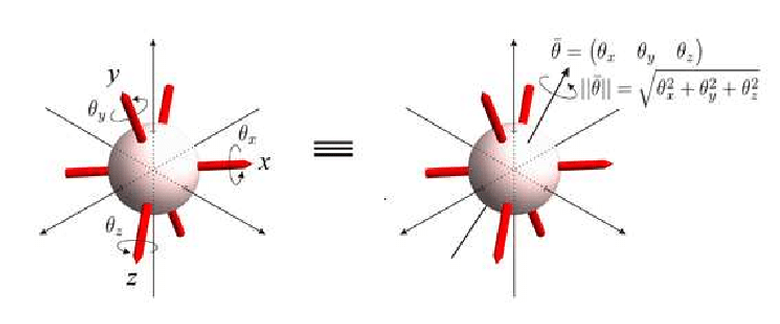
\includegraphics[width=0.5\linewidth]{figures/Rigid Body rotation.PNG}

    % Caption for List of Figures (no citation)
    \caption{Rigid body rotation in terms of axis-angle notation} \cite{guerrero2017quadrotor}

    % Caption shown only below the figure (with citation)
    %\caption*{Source: \cite{guerrero2017quadrotor}}

    \label{fig:Rigid Body rotation}
\end{figure}


And to get body frame velocity $\omega$ let’s take derivative of equation \eqref{3.5} from both sides:

\[
\omega = \frac{d\bar{\theta}}{dt} = \frac{d}{dt}(2 \ln q) 
= 2 \cdot \frac{1}{q} \otimes \dot{q} = 2 q^{-1} \otimes \dot{q}
\]

%\[
%\omega = 2 q^{-1} \otimes \dot{q}
%\]

Then by multiplying both sides with $\tfrac{1}{2}q$, and taking its derivative we have:

\begin{equation}
\dot{q} = \tfrac{1}{2} q \otimes \omega = \tfrac{1}{2} \big[ (q_0, \vec{q}) \otimes (0, \omega) \big] = \tfrac{1}{2} \big[ (q_0 \ast 0 - \vec{q}\cdot \omega,\; q_0 \ast \omega + 0 \ast \vec{q} + \vec{q} \times \omega ) \big]
%\tag{3.6}
\label{3.6}
\end{equation}

%By using equation \eqref{eqn:quaternion_product}, derivative of quaternion in equation \eqref{3.6} can be expanded as:
%\[
%\dot{q} = (\dot{q}_0, \dot{\vec{q}}) 
%= \tfrac{1}{2} q \otimes \omega 
%= \tfrac{1}{2} \big[ (q_0, \vec{q}) \otimes (0, \omega) \big] 
%\]

%\[
%(\dot{q}_0, \dot{\vec{q}}) 
%= \tfrac{1}{2} \big[ (q_0 \ast 0 - \vec{q}\cdot \omega,\; q_0 \ast \omega + 0 \ast \vec{q} + \vec{q} \times \omega ) \big]
%\]

% Force equation counter to 11 so next is 3.12
%\setcounter{equation}{6}


%\[
\begin{equation}
\dot{q}_0 = -\frac{1}{2}\,\vec{q}\cdot \omega \\
\dot{\vec{q}} = \frac{1}{2}\left(q_0\omega + \vec{q}\times\omega\right)
\label{3.7}
\end{equation}

%\end{cases}
%\]




Where $\,\omega=[p,q,r]^{T}\,$ is angular velocity in BF.

By expanding equation \eqref{3.7}, we can obtain the following equations for quaternion rates:

%\[\dot q_0=-\tfrac{1}{2}\big([q_1,q_2,q_3]\!\cdot\![p,q,r]\big)
%= -\tfrac{1}{2}\,(p q_1+q q_2+r q_3)\]

%\[
%\dot{\vec q}=\tfrac{1}{2}\,(q_0\omega+\vec q\times\omega)
%=\tfrac{1}{2}\!\left(
%\begin{bmatrix} q_0 \\[2pt] q_0 \\[2pt] q_0 \end{bmatrix}\!\odot\!\begin{bmatrix} p\\ q\\ r \end{bmatrix}
%+\begin{bmatrix} q_1\\ q_2\\ q_3 \end{bmatrix}\!\times\!\begin{bmatrix} p\\ q\\ r \end{bmatrix}
%\right)
%=\tfrac{1}{2}\!\left(
%\begin{bmatrix} p q_0\\ q q_0\\ r q_0 \end{bmatrix}
%+
%\begin{bmatrix} r q_2-q q_3\\ p q_3-r q_1\\ q q_1-p q_2 \end{bmatrix}
%\right)
%=\tfrac{1}{2}
%\begin{bmatrix}
%p q_0+r q_2-q q_3\\
%q q_0+p q_3-r q_1\\
%r q_0+q q_1-p q_2
%\end{bmatrix}\]

%\[\dot q_0=-\tfrac{1}{2}\big([q_1,q_2,q_3]\!\cdot\![p,q,r]\big)
%= -\tfrac{1}{2}\,(p q_1+q q_2+r q_3)\]
\begin{small}
    \[
\dot{\vec q}=\tfrac{1}{2}\,(q_0\omega+\vec q\times\omega)
=\tfrac{1}{2}\!\left(
\begin{bmatrix} q_0 \\[2pt] q_0 \\[2pt] q_0 \end{bmatrix}\!\odot\!\begin{bmatrix} p\\ q\\ r \end{bmatrix}
+\begin{bmatrix} q_1\\ q_2\\ q_3 \end{bmatrix}\!\times\!\begin{bmatrix} p\\ q\\ r \end{bmatrix}
\right)
=\tfrac{1}{2}\!\left(
\begin{bmatrix} p q_0\\ q q_0\\ r q_0 \end{bmatrix}
+
\begin{bmatrix} r q_2-q q_3\\ p q_3-r q_1\\ q q_1-p q_2 \end{bmatrix}
\right)
=\tfrac{1}{2}
\begin{bmatrix}
p q_0+r q_2-q q_3\\
q q_0+p q_3-r q_1\\
r q_0+q q_1-p q_2
\end{bmatrix}
\]

\end{small}



Hence, relation between quaternion rates and BF angular velocities is summarized as
\begin{equation}
\begin{bmatrix}
\dot q_0\\ \dot q_1\\ \dot q_2\\ \dot q_3
\end{bmatrix}
=\tfrac{1}{2}
\begin{bmatrix}
 q_0 & -q_1 & -q_2 & -q_3\\
 q_1 &  q_0 & -q_3 &  q_2\\
 q_2 &  q_3 &  q_0 & -q_1\\
 q_3 & -q_2 &  q_1 &  q_0
\end{bmatrix}
\begin{bmatrix}
0\\ p\\ q\\ r
\end{bmatrix}
%\tag{3.8}
\label{3.8}
\end{equation}


Where : 
\begin{equation}
\begin{bmatrix}
p \\ q \\ r
\end{bmatrix}
=
\begin{bmatrix}
1 & 0 & -s_\theta \\
0 & c_\phi & s_\phi c_\theta \\
0 & -s_\phi & c_\phi c_\theta
\end{bmatrix}
\begin{bmatrix}
\dot{\phi} \\ \dot{\theta} \\ \dot{\psi}
\end{bmatrix}
%\tag{3.8a}
\label{3.8a}
\end{equation}

\subsection{Mathematical Modeling of Quadrotor Dynamics}

%Since almost all systems in real life are nonlinear in nature, Control Engineers design either linear controller by linearizing those nonlinear systems at some operating point; or they design nonlinear controller based on simplified nonlinear model of the system by ignoring some features which are assumed to have less effect on the system. During simulation, the designed controller may show promising results by effectively driving tracking error toward zero. However, when we implement the developed control algorithm in the real system, the error may be diverged rather than converged toward zero. This is due to the designed control law, which is designed based on linearized/simplified model not based on the real plant, so unmodeled dynamics, which are neglected during modeling, may decrease controller performance and also they may cause the system unstable. 

Most real world systems are inherently nonlinear. Control engineers address this challenge through two primary approaches: designing linear controllers by linearizing the nonlinear system at an operating point, or developing nonlinear controllers based on simplified models that omit features with negligible effects. Although simulations typically show excellent performance with tracking errors converging to zero, implementation on actual systems often reveals divergent error behavior. This performance gap occurs because controllers are designed using linearized or simplified models rather than the true plant dynamics. The unmodeled dynamics, neglected during model development, can substantially reduce controller effectiveness and may even cause system instability. To mitigate the adverse effects of unmodeled dynamics, this section introduces a more realistic representation of the quadrotor system by incorporating all factors that significantly influence its dynamic behavior. This approach is motivated by a fundamental principle in control engineering, improving the accuracy of the system model generally enhances controller performance, even though it may increase the overall complexity of the model.

%To solve such harmful effect of unmodeled dynamics, in this section more realistical behavior of Quadrotor is enforced by considering every effect which has significant effect on the Quadrotor dynamics. This point is raised from general fact of Control Engineering arena which is when we design the model more accurately, controller performance will be increased though complexity of the model is increased.% As we will see later, due to high generalization capability of ANN, designed complex system model will be first represented by ANN model via system identification process; then based on the estimated model controller will be designed.

\bigskip

In order to derive mathematical model of Quadrotor dynamics, it is important to take the following assumptions \cite{doukhi2017intelligent},\cite{baoying2020research}, Structure of the Quadrotor is rigid with constant mass and uniform symmetry, gravitational force doesn’t change with altitude,quadrotor center of mass coincides with its geometric center,the resistance and inductance of BLDC motor are negligible, and at hovering position velocity of air and propellers are equal.

%\begin{enumerate}
   % \item Structure of the Quadrotor is rigid with constant mass and uniform symmetry,
   % \item Gravitational force doesn’t change with altitude,
   % \item Quadrotor center of mass coincides with its geometric center,
    %\item The resistance and inductance of BLDC motor are negligible, and
   % \item At hovering position velocity of air and propellers are equal.
%\end{enumerate}

\noindent
%Since Quadrotor structure is assumed to be rigid body, we can use Newtons laws to derive its dynamics. In the following subsections mathematical model of Quadrotor will be derived first by applying Newton-Euler approach and Newton-Quaternion approach for fully actuated rotational and underactuated translational dynamics based on Free Body Diagram (FBD) of Quadrotor as shown in figure\ref{fig:Quadrotor free body diagram}. Then, by comparing the two approaches, the best of the two approaches will be taken to develop appropriate model for realtime implementation and to enhance controller performance.

Since the quadrotor structure is assumed to behave as a rigid body, its dynamics can be derived using Newton’s laws of motion. In the following subsections, the mathematical model of the quadrotor is developed using the Newton--Quaternion approach to represent the system dynamics. This formulation is used to describe the fully actuated rotational dynamics and the underactuated translational dynamics based on the free body diagram (FBD) of the quadrotor shown in Figure~\ref{fig:Quadrotor free body diagram}. The quaternion-based representation provides an effective framework for modeling the quadrotor attitude dynamics and is suitable for real-time implementation and improved controller performance.



\subsubsection{Quadrotor Rotational Motion}

%By using Newton $2^{nd}$ law of rotational motion for fully actuated Quadrotor rotational dynamics, the net moment derived from BF as follows:
By applying Newton's $2^{\text{nd}}$ law of rotational motion to the fully actuated rotational dynamics of the quadrotor, the resultant moment acting on the system can be derived from the body frame (BF) as follows:

\begin{equation}
\sum \tau_i = J \alpha = [U_2, U_3, U_4]^T - M_{gyro} - M_{aero}
%\tag{3.9}
\label{3.9}
\end{equation}

Where: $J =$ inertia matrix. 
$\alpha = [\dot{p}, \dot{q}, \dot{r}]^T$ are angular accelerations in BF; 
$U_2, U_3,$ and $U_4$ are moments on BF which are used to control roll, pitch, and yaw, respectively; 
$M_{gyro} =$ gyroscopic moment, and 
$M_{aero} =$ aerodynamic frictional moment.

\paragraph{Inertia Matrix of the Quadrotor}

%\subsubsubsection{Inertia Matrix of the Quadrotor}
%Actual inertia matrix of Quadrotor is assumed to be constant matrix,
%since structure of a Quadrotor is assumed to be symmetrical with respect to coordinate system, 
%$J_{xy} = J_{xz} = J_{yz} = 0$ and $J_{xx} = J_{yy}$~\cite{beard2008quadrotor}. 
%Hence, inertia matrix for Quadrotor now becomes a diagonal matrix. Where: $J_{xx}, J_{yy},$ and $J_{zz}$ are moments of inertia about the principal axis on the BF.
The inertia matrix of the quadrotor is assumed to be constant. Since the quadrotor structure is considered symmetric with respect to the coordinate axes, the products of inertia satisfy $J_{xy}=J_{xz}=J_{yz}=0$, and the moments of inertia about the $x$ and $y$ axes are equal, i.e., $J_{xx}=J_{yy}$~\cite{beard2008quadrotor}. Consequently, the inertia matrix of the quadrotor reduces to a diagonal form. Here, $J_{xx}$, $J_{yy}$, and $J_{zz}$ represent the moments of inertia about the principal axes of the body frame (BF).

\begin{equation}
J =
\begin{bmatrix}
J_{xx} & -J_{xy} & -J_{xz} \\
-J_{xy} & J_{yy} & -J_{yz} \\
-J_{xz} & -J_{yz} & J_{zz}
\end{bmatrix} J =
\begin{bmatrix}
J_{xx} & 0 & 0 \\
0 & J_{yy} & 0 \\
0 & 0 & J_{zz}
\end{bmatrix}
%\tag{3.10}
\label{3.10} 
\end{equation}
%\[

%\]



%Since structure of a Quadrotor is assumed to be symmetrical with respect to coordinate system, 
%$J_{xy} = J_{xz} = J_{yz} = 0$ and $J_{xx} = J_{yy}$~\cite{beard2008quadrotor}. 
%Hence, inertia matrix for Quadrotor now becomes a diagonal matrix:

%\begin{equation}
%J =
%\begin{bmatrix}
%J_{xx} & 0 & 0 \\
%0 & J_{yy} & 0 \\
%0 & 0 & J_{zz}
%\end{bmatrix}
%\tag{3.10}
%\label{3.10}
%\end{equation}

%Where: $J_{xx}, J_{yy},$ and $J_{zz}$ are moments of inertia about the principal axis on the BF.

\paragraph*{Euler’s Equations of Rigid Body Dynamics}

%Euler’s rotation equations is a vector quasi-linear first order ordinary differential equation which describe the rotation of a Quadrotor in BF w.r.t IF. Let the unit vectors $\vec{i}, \vec{j},$ or $\vec{k}$ representing standard basis of unit vectors in the rotating BF. If they are rotating at the speed of $\omega$ w.r.t fixed IF, then time derivative of each rotating coordinate frame: $\vec{i}, \vec{j},$ or $\vec{k}$ of unit vector $\vec{u}$ becomes:

Euler's rotational equations form a vector quasi-linear first-order ordinary differential equation that describes the rotational motion of a quadrotor in the body frame (BF) with respect to the inertial frame (IF). Let the unit vectors $\vec{i}$, $\vec{j}$, and $\vec{k}$ denote the standard basis vectors of the rotating body frame. If the body frame rotates with an angular velocity $\omega$ relative to the fixed inertial frame, then the time derivative of each rotating unit vector $\vec{i}$, $\vec{j}$, and $\vec{k}$, represented generically by the unit vector $\vec{u}$, can be expressed as follows:


\begin{equation}
    \frac{d}{dt}\vec{u} = \omega \times \vec{u}
\end{equation}



%Since both angular acceleration and angular velocity of Quadcopter are vector quantities, both their magnitudes and directions in rotating BF are change in with time w.r.t fixed IF. Therefore, by using chain rule we have the following expression for net moment of Quadrotor:

Since the angular velocity and angular acceleration of the quadrotor are vector quantities, their magnitudes and directions in the rotating body frame (BF) vary with time relative to the inertial frame (IF). Therefore, by applying the chain rule, the net moment of the quadrotor can be expressed as follows:

%\[
\begin{equation}
J\alpha = J \frac{d}{dt}(\omega \vec{u}) 
= J \frac{d\omega}{dt}\vec{u} + \frac{d}{dt}(J\omega \vec{u})
= J \frac{d\omega}{dt}\vec{u} + \omega \times (J\omega \vec{u})
= J \frac{d\omega}{dt} + \omega \times (J\omega) = J\dot{\omega} + \omega \times (J\omega)
\label{3.11}
\end{equation}

%\]

%\begin{equation}
%J\alpha = J\dot{\omega} + \omega \times (J\omega)
%\tag{3.11}
%\label{3.11}
%\end{equation}

%Where: $\omega = \omega \vec{u} = [p, q, r]^T$ which represents Euler angular rates in Quadrotor BF.



\subsubsection{Gyroscopic Effect of Propellers}

The spinning propellers induces a gyroscopic torque when the Quad rotates in the space~\cite{selfridge2014multivariable}.
This induced torque act on the axis which is perpendicular to stationary axes of propellers rotation
and axes of Quad body rotation along x-axis or y-axis, and it is expressed as:

\begin{equation}
    M_{gyro} = J_p \Omega \times \omega
    %\tag{3.12}
    \label{3.12}
\end{equation}

Where $\omega$ is speed of Quad body rotates along x or y axis, $\Omega$ is angular speed of propellers,
and $J_p$ is inertia of propeller. Since a Quad has four propellers or rotors, we need to solve the
gyro induced torque separately four times along x-axis and four times along y-axis. Based on
Figure~\ref{fig:Quadrotor free body diagram} propeller 2 and 4 rotates in CCW direction, and 1 and 3 in CW direction, the resultant
gyroscopic moment along x-axis: $M_{x_{gyro}}$, and y-axis: $M_{y_{gyro}}$ expressed as follows:

\begin{equation}
    M_{x_{gyro}} = J_p q \Omega_r %\tag{3.13}
    \label{3.13}
\end{equation}

\begin{equation}
    M_{y_{gyro}} = -J_p p \Omega_r %\tag{3.14}
    \label{3.14}
\end{equation}

Where: $\Omega_r = -\Omega_1 + \Omega_2 - \Omega_3 + \Omega_4$ is the net angular velocity of the
propellers and $\Omega_i$ ($i=1,2,3,4$) is velocity of each propeller. Equation~\eqref{3.13} implies that
induced torque about x-axis due to angular rate of change to pitch $q$, i.e. a Quad will feel a body
roll-induced torque when it pitches; this is due to the gyroscopic effect of the four propellers.
The same thing is expressed in Equation~\eqref{3.14} for y-axis induced gyroscopic torque. Rotation about
z-axis contributes no gyroscopic effect from the propellers rotation because the axis of propellers
rotation and vehicle rotation axis pointing in the same direction, so the cross product becomes zero,
i.e., no torque is induced during yaw or z-axis rotation.

\subsubsection{Aerodynamic Effects due to Propellers Rotation}

This is also known as viscous frictional torque in BF resulting from aerodynamic friction, 
and it’s given as~\cite{bensalah2019full}:

\begin{equation}
    M_{aero} = C_a \omega %\tag{3.15}
    \label{3.15}
\end{equation}

% --- context line above the derivation (optional) ---
Where $C_a$ is an aerodynamic coefficient depending on air density and the angular speed of the
quadrotor $\omega$.

By substituting equation \eqref{3.11}-\eqref{3.15} in Eq.\eqref{3.9}, rotational dynamics of Quadrotor is
derived as follows:
\begin{small}
\begin{equation}
\begin{align*}
J \alpha &= [U_2, U_3, U_4]^T - M_{gyro} - M_{aero} \\[6pt]
J\dot{\omega} + \omega \times (J\omega) &= [U_2, U_3, U_4]^T - M_{gyro} - M_{aero} \\[6pt]
\dot{\omega} &= J^{-1} \Big( [U_2, U_3, U_4]^T - \omega \times (J\omega) - M_{gyro} - M_{aero} \Big)
\end{align*} 
\end{equation}


%\begin{align*}
%J \alpha &= [U_2, U_3, U_4]^T - M_{gyro} - M_{aero} \\[6pt]
%J\dot{\omega} + \omega \times (J\omega) &= [U_2, U_3, U_4]^T - M_{gyro} - M_{aero} \\[6pt]
%\dot{\omega} &= J^{-1} \Big( [U_2, U_3, U_4]^T - \omega \times (J\omega) - M_{gyro} - M_{aero} \Big)
%\end{align*}

\begin{align*}
\begin{bmatrix} \dot{p} \\ \dot{q} \\ \dot{r} \end{bmatrix}
&=
\begin{bmatrix}
J_{xx} & 0 & 0 \\
0 & J_{yy} & 0 \\
0 & 0 & J_{zz}
\end{bmatrix}^{-1}
\left(
\begin{bmatrix} U_2 \\ U_3 \\ U_4 \end{bmatrix}
-
\begin{bmatrix} p \\ q \\ r \end{bmatrix}
\times
\begin{bmatrix}
J_{xx} & 0 & 0 \\
0 & J_{yy} & 0 \\
0 & 0 & J_{zz}
\end{bmatrix}
\begin{bmatrix} p \\ q \\ r \end{bmatrix}
-
\begin{bmatrix}
J_p q \Omega_r - C_a p \\
- J_p p \Omega_r - C_a q \\
C_a r
\end{bmatrix}
%\right) \\[8pt]
%&=
%\begin{bmatrix}
%\frac{1}{J_{xx}} & 0 & 0 \\
%0 & \frac{1}{J_{yy}} & 0 \\
%0 & 0 & \frac{1}{J_{zz}}
%\end{bmatrix}
%\left(
%\begin{bmatrix} U_2 \\ U_3 \\ U_4 \end{bmatrix}
%-
%\begin{bmatrix} p \\ q \\ r \end{bmatrix}
%\times
%\begin{bmatrix}
%J_{xx}p \\ J_{yy}q \\ J_{zz}r
%\end{bmatrix}
%-
%\begin{bmatrix}
%J_p q \Omega_r + C_a p \\
%- J_p p \Omega_r + C_a q \\
%C_a r
%\end{bmatrix}
%\right) \\[8pt]
%&=
%\begin{bmatrix}
%\frac{1}{J_{xx}} & 0 & 0 \\
%0 & \frac{1}{J_{yy}} & 0 \\
%0 & 0 & \frac{1}{J_{zz}}
%\end{bmatrix}
%\left(
%\begin{bmatrix} U_2 \\ U_3 \\ U_4 \end{bmatrix}
%-
%\begin{bmatrix}
%(J_{zz}-J_{yy})qr \\
%(J_{xx}-J_{zz})pr \\
%(J_{yy}-J_{xx})pq
%\end{bmatrix}
%-
%\begin{bmatrix}
%J_p q \Omega_r + C_a p \\
%- J_p p \Omega_r + C_a q \\
%C_a r
%\end{bmatrix}
%\right) \\[8pt]
%&=
%\begin{bmatrix}
%\frac{1}{J_{xx}}\left( U_2 + (J_{yy}-J_{zz})qr - J_p q \Omega_r - C_a p \right) \\[6pt]
%\frac{1}{J_{yy}}\left( U_3 + (J_{zz}-J_{xx})pr + J_p p \Omega_r - C_a q \right) \\[6pt]
%\frac{1}{J_{zz}}\left( U_4 + (J_{xx}-J_{yy})pq - C_a r \right)
%\end{bmatrix}
\end{align*}

    
\end{small}



Hence,
% Set counter so next equation is 3.20
%\setcounter{equation}{19}

%\begin{subequations}
%\begin{empheq}[left=\empheqlbrace]{align}
%\dot{p} &= \tfrac{1}{J_{xx}} U_2
       % + \tfrac{J_{yy}-J_{zz}}{J_{xx}} qr
       % - \tfrac{J_p}{J_{xx}} q \Omega_r
        %- \tfrac{C_{a_p}}{J_{xx}} p \label{eq:320a}\\[1.1ex]
%\dot{q} &= \tfrac{1}{J_{yy}} U_3
        %+ \tfrac{J_{zz}-J_{xx}}{J_{yy}} pr
       % + \tfrac{J_p}{J_{yy}} p \Omega_r
       % - \tfrac{C_{a_q}}{J_{yy}} q \label{eq:320b}\\[1.1ex]
%\dot{r} &= \tfrac{1}{J_{zz}} U_4
       % + \tfrac{J_{xx}-J_{yy}}{J_{zz}} pq
       % - \tfrac{C_{a_r}}{J_{zz}} r \label{eq:320c}
%\end{empheq}
%\end{subequations}


\begin{equation}
\left\{
\begin{aligned}
\dot{p} &= \frac{1}{J_{xx}} U_2 
        + \frac{J_{yy}-J_{zz}}{J_{xx}}\, q r
        - \frac{J_p}{J_{xx}}\, q \Omega_r
        - \frac{C_{ap}}{J_{xx}}\, p, \\[6pt]
\dot{q} &= \frac{1}{J_{yy}} U_3
        + \frac{J_{zz}-J_{xx}}{J_{yy}}\, p r
        + \frac{J_p}{J_{yy}}\, p \Omega_r
        - \frac{C_{aq}}{J_{yy}}\, q, \\[6pt]
\dot{r} &= \frac{1}{J_{zz}} U_4
        + \frac{J_{xx}-J_{yy}}{J_{zz}}\, p q
        - \frac{C_{ar}}{J_{zz}}\, r
\end{aligned}
\right.
%\tag{3.16}
\end{equation}



\subsubsection{Quadrotor Translational Motion}

%Translational dynamics of Quadrotor is derived based on Newton 2\textsuperscript{nd} law of translational motion. Since Newton’s laws are valid only in IF, we use the rotation matrix which project thrust force that generated in BF into IF. In these scenario, translational dynamics of Quadrotor is derived in the following sub subsection based on Newton–Euler formalism and Newton–Quaternion formalism as follows:

Translational dynamics of Quadrotor is derived based on Newton 2\textsuperscript{nd} law of translational
motion. Since Newton’s laws are valid only in IF, we use the rotation matrix which project thrust
force that generated in BF into IF. In these scenario, translational dynamics of Quadrotor is derived
in  Newton–Quaternion formalism as follows:




\subsubsubsection{\textbf{Newton--Quaternion Formalism}}

By applying Newton--Quaternion approach, Quadrotor translational dynamics is derived as:
\begin{small}
\begin{equation}
    a = \frac{1}{m}\big[ R_b^{e} U_1 - F_g - F_d \big]
    \label{eq:translation dynamics}
\end{equation}

 Substituting Eqn \eqref{eqn 3.4}, gravity and drag forces  in Eqn \eqref{eq:translation dynamics} it is found to be:
%\[
%\begin{bmatrix}
%\ddot{x} \\[6pt]
%\ddot{y} \\[6pt]
%\ddot{z}
%\end{bmatrix}
%=
%\frac{1}{m}
%\left[
%\begin{bmatrix}
%2(q_0^2+q_1^2)-1 & 2(q_1q_2+q_0q_3) & 2(q_1q_3-q_0q_2) \\
%2(q_1q_2-q_0q_3) & 2(q_0^2+q_2^2)-1 & 2(q_2q_3+q_0q_1) \\
%2(q_0q_3+q_1q_2) & 2(q_2q_3-q_0q_1) & 2(q_0^2+q_3^2)-1
%\end{bmatrix}
%\begin{bmatrix}
%0 \\[4pt] 0 \\[4pt] U_1
%\end{bmatrix}
%-
%\begin{bmatrix}
%0 \\[4pt] 0 \\[4pt] mg
%\end{bmatrix}
%-
%\begin{bmatrix}
%C_{d_x}\dot{x} \\[4pt]
%C_{d_y}\dot{y} \\[4pt]
%C_{d_z}\dot{z}
%\end{bmatrix}
%\right]
%\]

%\[
%= \frac{1}{m}
%\begin{bmatrix}
%2(q_1q_3-q_0q_2)U_1 - C_{d_x}\dot{x} \\[6pt]
%2(q_2q_3+q_0q_1)U_1 - C_{d_y}\dot{y} \\[6pt]
%\big[2(q_0^2+q_3^2)-1\big]U_1 - mg - C_{d_z}\dot{z}
%\end{bmatrix}
%\]
 
%\end{small}



\begin{equation}
\left\{
\begin{aligned}
\ddot{x} &= 2(q_1 q_3 - q_0 q_2)\frac{U_1}{m}
           - \frac{C_{d_x}}{m}\dot{x} \\
\ddot{y} &= 2(q_2 q_3 + q_0 q_1)\frac{U_1}{m}
           - \frac{C_{d_y}}{m}\dot{y}  \\
\ddot{z} &= \Big[2(q_0^2 + q_3^2)-1\Big]\frac{U_1}{m}
           - g - \frac{C_{d_z}}{m}\dot{z} \\
\end{aligned}
\right.
%\tag{3.17}
\end{equation}

\subsubsection{Total Thrust Force and Moments Produced by Propellers}

%The rotor attains thrust by pushing air downward, so Newton’s equation $F=ma$ is used to
%equate thrust $T$ to the rate of momentum change of air: $ma = \tfrac{dp}{dt}$. 
%As air acceleration begins at some distance above the rotor and continues to some distance below the rotor, 
%from momentum theory of hovering state Quadrotor we have the following expression: 
%since $p = m\Omega$,

%\begin{equation*}
%T = \frac{dp}{dt} = \frac{d}{dt}(m\Omega)
%\end{equation*}

%But $m = \rho v$, and $v = AS \longrightarrow m = \rho AS$, then by substituting this in above equation we get

%\begin{equation*}
%T = \frac{d}{dt}(\rho AS\Omega) = \rho A \Omega \frac{dS}{dt}
%\end{equation*}

%Since $\frac{dS}{dt} = \Omega$ (which is constant since the Quad is at hovering state)

%\begin{equation*}
%T = \rho A \Omega^2
%\end{equation*}

%\begin{equation*}
%\Omega = \sqrt{\frac{T}{\rho A}}
%\end{equation*}


%Power $P$ at hovering is equal to thrust force times average velocity of propeller:

%\begin{equation*}
%P = T\Omega = T \sqrt{\frac{T}{\rho A}}
%\end{equation*}

%\begin{equation}
%P = \frac{T^{\tfrac{3}{2}}}{\sqrt{\rho A}}
%\tag{3.18}
%\label{3.18}
%\end{equation}

%Where $\rho$ is air density, $v$ is volume, $S$ is distance, $A$ is cross-sectional area of Quadrotor, 
%and $\Omega$ is velocity of rotor or air at hovering state. 
%By using equation~\eqref{3.18}, power used by BLDC motor to generate corresponding thrust force can be determined.

%%%%%%%%%%%%%%%%
The thrust generated by a rotor results from accelerating air downward. 
According to Newton’s second law, thrust is equal to the rate of change of momentum of the airflow

\begin{equation}
T = \frac{dp}{dt} 
\end{equation}

where $p$ is the momentum of the air. Since momentum is the product of mass and velocity,

\begin{equation}
p = m\Omega
\end{equation}

the thrust can be written as

\begin{equation}
T = \frac{d}{dt}(m\Omega)
\end{equation}

The mass of air passing through the rotor disk is expressed as

\begin{equation}
m = \rho V
\end{equation}

where $\rho$ is the air density and $V$ is the volume of air. 
For a rotor disk of area $A$ and airflow displacement $S$, the volume is $V = AS$, thus

\begin{equation}
m = \rho AS
\end{equation}

Substituting into the momentum equation yields

\begin{equation}
T = \frac{d}{dt}(\rho AS\Omega)
\end{equation}

Assuming constant air density and rotor area,

\begin{equation}
T = \rho A \Omega \frac{dS}{dt}
\end{equation}

At hover, the air velocity through the rotor disk is constant, therefore

\begin{equation}
\frac{dS}{dt} = \Omega
\end{equation}

which leads to

\begin{equation}
T = \rho A \Omega^2
\end{equation}

Hence, the induced velocity is

\begin{equation}
\Omega = \sqrt{\frac{T}{\rho A}}
\end{equation}

The power required during hovering is the product of thrust and induced velocity

\begin{equation}
P = T\Omega
\end{equation}

Substituting the induced velocity gives

\begin{equation}
P = \frac{T^{\tfrac{3}{2}}}{\sqrt{\rho A}}
\label{3.18}
\end{equation}

where $\rho$ is the air density, $A$ is the rotor disk area, $S$ is the airflow displacement, 
and $\Omega$ is the induced air velocity at hover. Using equation~\eqref{3.18}, the power 
required by the BLDC motor to generate the corresponding thrust can be determined.




%%%%%%%%%%%%

\subsubsubsection{\textbf{Actuators Dynamics}}

%Since the voltage equation of a trapezoidal BLDC motor is similar to that of a DC motor, 
%Kirchhoff’s Voltage Law (KVL) applied to the per–phase equivalent circuit shown in 
%Figure~\ref{fig:BLDC MOTOR} gives

%\begin{equation}
%V_a = R_a i_a + L_a \frac{di_a}{dt} + e_b
%\end{equation}

%where $R_a$, $L_a$ and $i_a$ are the stator resistance,   inductance and armature current, respectively. 
%The back electromotive force $e_b$  is

%\begin{equation}
%e_b = K_v \Omega
%\end{equation}

%with $\Omega$ and $K_v$ representing the rotor angular velocity and voltage constant respectively. 
%Assuming that the stator resistance and inductance are negligible, the voltage equation reduces to Terminal voltage $V_a$ as

%\begin{equation}
%V_a = e_b = K_v \Omega
%\end{equation}

\begin{figure}[h!]
    \centering
    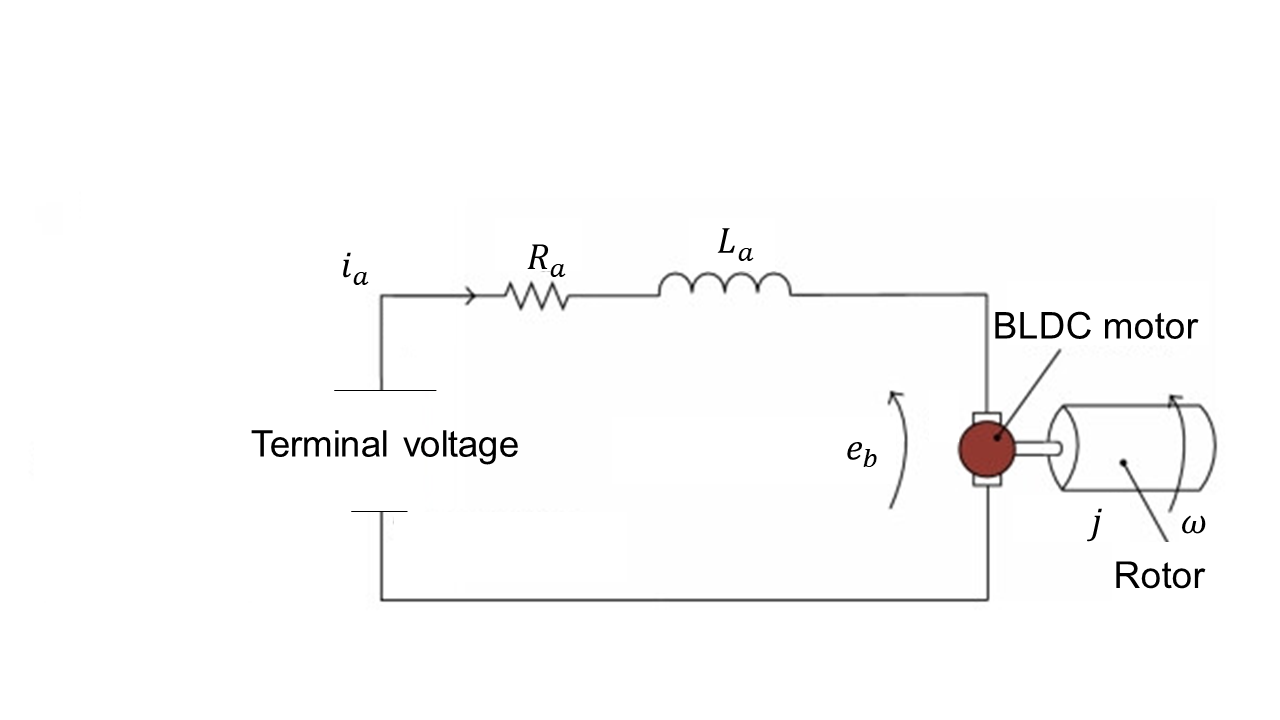
\includegraphics[width=0.5\linewidth]{figures/per phase circuit of BLDC.png}

    \caption{Per phase equivalent circuit of a trapezoidal BLDC motor } %\cite{xiang2015practical}
    %\caption*{Source: \cite{xiang2015practical}}

    \label{fig:BLDC MOTOR}
\end{figure}

%The motor torque is proportional to the armature current,

%\begin{equation*}
%\tau_m = K_\tau i_a
%\end{equation*}

%thus

%\begin{equation*}
%i_a = \frac{\tau_m}{K_\tau}
%\end{equation*}

%The electrical power consumed at hovering is

%\begin{equation*}
%P = V_a i_a = K_v \Omega \frac{\tau_m}{K_\tau}
%\end{equation*}

%Assuming the motor torque is proportional to the generated thrust, i.e., 
%$\tau_m = K_t T$, the power becomes

%\begin{equation}
%P = \frac{K_v}{K_\tau} K_t T \Omega
%\label{3.19}
%\end{equation}

%Combining equation~\eqref{3.18} with equation~\eqref{3.19} yields

%\begin{equation*}
%\frac{T^{\tfrac{3}{2}}}{\sqrt{\rho A}} = \frac{K_v}{K_\tau} K_t T \Omega
%\end{equation*}

%which simplifies to

%\begin{equation*}
%T^{\tfrac{1}{2}} = \frac{K_v}{K_\tau} K_t \sqrt{\rho A} \, \Omega
%\end{equation*}

%Squaring both sides gives

%\begin{equation*}
%T = \left[ \frac{K_v}{K_\tau} K_t \sqrt{\rho A} \right]^2 \Omega^2
%\end{equation*}

%Let

%\[
%b = \left[ \frac{K_v}{K_\tau} K_t \sqrt{\rho A} \right]^2
%\]

%where $b$ denotes the thrust coefficient. Hence,

%\begin{equation}
%T = b \Omega^2
%\label{3.20}
%\end{equation}


%%%%%%%%%%%%%%%%%%%%%%%%%%%
The actuator dynamics of the propeller motor assembly can be derived from the electrical and electromechanical relationships of the trapezoidal BLDC motor. Since the voltage equation of a trapezoidal BLDC motor is similar to that of a conventional DC motor, Kirchhoff’s Voltage Law (KVL) applied to the per phase equivalent circuit shown in Figure~\ref{fig:BLDC MOTOR} gives
\begin{equation}
V_a = R_a i_a + L_a \frac{di_a}{dt} + e_b
\end{equation}
where $V_a$ is the applied terminal voltage (V), $R_a$ is the stator phase resistance ($\Omega$), $L_a$ is the stator phase inductance (H), $i_a$ is the stator current (A), and $e_b$ is the back electromotive force (V).

The back electromotive force is proportional to the rotor angular velocity and is expressed as
\begin{equation}
e_b = K_v \Omega
\end{equation}
where $K_v$ is the back electromotive force (EMF)  constant (V\,s/rad) and $\Omega$ is the rotor angular velocity (rad/s).

Under steady state operation and for a simplified actuator model, the voltage drops across the stator resistance and inductance are assumed negligible compared to the back-EMF. Therefore, the voltage equation reduces to
\begin{equation}
V_a \approx e_b = K_v \Omega
\end{equation}

The electromagnetic torque produced by the motor is proportional to the stator current, that is,
\begin{equation}
\tau_m = K_{\tau} i_a
\end{equation}
where $\tau_m$ is the motor electromagnetic torque (N\,m) and $K_{\tau}$ is the motor torque constant (N\,m/A). Rearranging gives
\begin{equation}
i_a = \frac{\tau_m}{K_{\tau}}
\end{equation}

The electrical power consumed by the motor during hovering is given by
\begin{equation}
P = V_a i_a
\end{equation}
where $P$ is the electrical input power (W). Substituting $V_a = K_v \Omega$ and $i_a = \tau_m / K_{\tau}$ yields
\begin{equation}
P = K_v \Omega \frac{\tau_m}{K_{\tau}}
\end{equation}

For the propeller motor system, the motor torque is assumed proportional to the generated thrust. Thus,
\begin{equation}
\tau_m = K_t T
\end{equation}
where $K_t$ is the torque thrust proportionality constant and $T$ is the thrust generated by the propeller (N). Substituting this relation into the power expression gives
\begin{equation}
P = \frac{K_v}{K_{\tau}} K_t T \Omega
\label{eq:motor_power}
\end{equation}

On the other hand, from momentum theory, the aerodynamic power required to generate thrust can be expressed as
\begin{equation}
P = \frac{T^{3/2}}{\sqrt{\rho A}}
\label{eq:aero_power}
\end{equation}
where $\rho$ is the air density (kg/m$^3$) and $A$ is the rotor disc area (m$^2$).

Combining \eqref{eq:aero_power} and \eqref{eq:motor_power} gives
\begin{equation}
\frac{T^{3/2}}{\sqrt{\rho A}} = \frac{K_v}{K_{\tau}} K_t T \Omega
\end{equation}

Dividing both sides by $T$ results in
\begin{equation}
T^{1/2} = \frac{K_v}{K_{\tau}} K_t \sqrt{\rho A}\,\Omega
\end{equation}

Squaring both sides gives
\begin{equation}
T = \left( \frac{K_v}{K_{\tau}} K_t \sqrt{\rho A} \right)^2 \Omega^2
\end{equation}

Let
\begin{equation}
b = \left( \frac{K_v}{K_{\tau}} K_t \sqrt{\rho A} \right)^2
\end{equation}
where $b$ denotes the lumped thrust coefficient. Hence, the thrust generated by the propeller is obtained as
\begin{equation}
T = b \Omega^2
\label{3.20}
\end{equation}

Equations~\eqref{eq:motor_power}--\eqref{3.20} show that the thrust produced by the BLDC motor--propeller actuator is proportional to the square of the rotor angular velocity. This relationship is commonly used in quadrotor dynamic modeling and control design.


%%%%%%%%%%%%%%%%%%%%%%%%

Equation~\eqref{3.20} shows that the thrust produced by each propeller is proportional 
to the square of its angular speed. Using equations~\eqref{3.18} and~\eqref{3.20}, the 
relationship among propeller speed, thrust, and power can be determined. Consequently, 
the required power delivered by the Electronic Speed Controller (ESC) to the BLDC motor 
can be estimated in order to achieve the desired propeller speed and generate the thrust 
necessary to drive the quadrotor according to the commanded input.




%%%%%%%%%%%%%%%%%%%%%



\subsubsubsection{\textbf{Total Thrust Force and Moments Derivation}}

Based on free body diagram of Quadrotor in Figure\ref{fig:Quadrotor free body diagram} and equation \eqref{3.20}, 
\textbf{total thrust force} $U_1$ due to rotation of each propeller is solved as follows: 
Since all the thrust forces are acting in upward direction:

\begin{equation}
U_1 = T_1 + T_2 + T_3 + T_4 = b\Omega_1^2 + b\Omega_2^2 + b\Omega_3^2 + b\Omega_4^2 = b(\Omega_1^2 + \Omega_2^2 + \Omega_3^2 + \Omega_4^2)
\label{3.21}
\end{equation}
%\end{equation*}

%\begin{equation}
%U_1 = b(\Omega_1^2 + \Omega_2^2 + \Omega_3^2 + \Omega_4^2)
%\tag{3.21}
%\label{3.21}
%\end{equation}

The \textbf{rolling control torque} $U_2$ in positive $\phi$ direction is solved as follows:

\begin{equation}
U_2 = \ell (T_1 - T_2 - T_3 + T_4) 
    = \ell (b\Omega_1^2 - b\Omega_2^2 - b\Omega_3^2 + b\Omega_4^2)  = \ell b(\Omega_1^2 - \Omega_2^2 - \Omega_3^2 + \Omega_4^2)
    \label{3.22}
\end{equation}


Where $\ell$ is distance between rotor center and CoG of Quadrotor, and the positive and 
negative sign indicate the rotor at which their speed increase and decrease, respectively, 
in the way that maintaining the overall thrust $U_1$ constant.

%\begin{equation}
%U_2 = \ell b(\Omega_1^2 - \Omega_2^2 - \Omega_3^2 + \Omega_4^2)
%\tag{3.22}
%\label{3.22}
%\end{equation}

The \textbf{pitching control torque} $U_3$ in positive $\theta$ direction is solved as follows:

\begin{equation}
U_3 = \ell (T_1 + T_2 - T_3 - T_4) 
    = \ell (b\Omega_1^2 + b\Omega_2^2 - b\Omega_3^2 - b\Omega_4^2) = \ell b(\Omega_1^2 + \Omega_2^2 - \Omega_3^2 - \Omega_4^2)
%\tag{3.23}
\label{3.23}
\end{equation}

%\begin{equation}
%U_3 = \ell b(\Omega_1^2 + \Omega_2^2 - \Omega_3^2 - \Omega_4^2)
%\tag{3.23}
%\label{3.23}
%\end{equation}


The \textbf{yaw control torque} $U_4$ is solved based on the concept of Newton third law of motion, 
which states that for any action torque there is reactive torque generated by drag torque $\tau_i (i=1,2,3,4)$. 
Due to this drag torque, yaw rotation is caused in the direction of net drag torque. 
For instance, if $(\tau_2 + \tau_4) > (\tau_1 + \tau_3)$, the Quad will rotate in positive yaw direction. 
In the same way as equation \eqref{3.20}, drag torque mathematically formulated as $\tau = d\Omega^2$, 
where $d$ is aerodynamic drag coefficient. Hence, yaw control torque becomes:

\begin{equation}
U_4 = d(-\Omega_1^2 + \Omega_2^2 - \Omega_3^2 + \Omega_4^2)
%\tag{3.24}
\label{3.24}
\end{equation}

By combining equations \eqref{3.21}-\eqref{3.24}, control mixing matrix is derived as follows:

\begin{equation}
\begin{bmatrix}
U_1 \\[6pt]
U_2 \\[6pt]
U_3 \\[6pt]
U_4
\end{bmatrix}
=
\begin{bmatrix}
b   & b   & b   & b   \\[6pt]
b\ell & -b\ell & -b\ell & b\ell \\[6pt]
b\ell & b\ell & -b\ell & -b\ell \\[6pt]
-d  & d   & -d  & d
\end{bmatrix}
\begin{bmatrix}
\Omega_1^2 \\[6pt]
\Omega_2^2 \\[6pt]
\Omega_3^2 \\[6pt]
\Omega_4^2
\end{bmatrix}    
\end{equation}

%\]


By using \textbf{Symbolic Math Toolbox}$^{\text{TM4}}$ in MATLAB$^{\text{\textregistered}}$, 
Then, \textbf{Control allocation or mixing} equations become:

%\[
%\begin{bmatrix}
%\Omega_1^2 \\[8pt]
%\Omega_2^2 \\[8pt]
%\Omega_3^2 \\[8pt]
%\Omega_4^2
%\end{bmatrix}
%=
%\begin{bmatrix}
%\dfrac{1}{4b} & \dfrac{1}{4b\ell} & \dfrac{1}{4b\ell} & -\dfrac{1}{4d} \\[12pt]
%\dfrac{1}{4b} & -\dfrac{1}{4b\ell} & \dfrac{1}{4b\ell} & \dfrac{1}{4d} \\[12pt]
%\dfrac{1}{4b} & -\dfrac{1}{4b\ell} & -\dfrac{1}{4b\ell} & -\dfrac{1}{4d} \\[12pt]
%\dfrac{1}{4b} & \dfrac{1}{4b\ell} & -\dfrac{1}{4b\ell} & \dfrac{1}{4d}
%\end{bmatrix}
%\begin{bmatrix}
%U_1 \\[8pt]
%U_2 \\[8pt]
%U_3 \\[8pt]
%U_4
%\end{bmatrix}
%\]


%Then, \textbf{Control allocation or mixing} equations become:

%\begin{subequations}
 % \renewcommand\theequation{3.30\alph{equation}} % -> (3.30a–d)
 % \begin{empheq}[left=\empheqlbrace]{align}
   % \Omega_1 &= \sqrt{\tfrac{U_1}{4b} + \tfrac{U_2}{4b\ell} + \tfrac{U_3}{4b\ell} - \tfrac{U_4}{4d}} \label{eq:330a}\\[8pt]
   % \Omega_2 &= \sqrt{\tfrac{U_1}{4b} - \tfrac{U_2}{4b\ell} + \tfrac{U_3}{4b\ell} + \tfrac{U_4}{4d}} \label{eq:330b}\\[8pt]
    %\Omega_3 &= \sqrt{\tfrac{U_1}{4b} - \tfrac{U_2}{4b\ell} - \tfrac{U_3}{4b\ell} - \tfrac{U_4}{4d}} \label{eq:330c}\\[8pt]
    %\Omega_4 &= \sqrt{\tfrac{U_1}{4b} + \tfrac{U_2}{4b\ell} - \tfrac{U_3}{4b\ell} + \tfrac{U_4}{4d}} \label{eq:330d}
  %\end{empheq}
%\end{subequations}

\begin{equation}
\left\{
\begin{aligned}
 \Omega_1 &= \sqrt{\tfrac{U_1}{4b} + \tfrac{U_2}{4b\ell} + \tfrac{U_3}{4b\ell} - \tfrac{U_4}{4d}} \\[8pt]
    \Omega_2 &= \sqrt{\tfrac{U_1}{4b} - \tfrac{U_2}{4b\ell} + \tfrac{U_3}{4b\ell} + \tfrac{U_4}{4d}} \\[8pt]
    \Omega_3 &= \sqrt{\tfrac{U_1}{4b} - \tfrac{U_2}{4b\ell} - \tfrac{U_3}{4b\ell} - \tfrac{U_4}{4d}} \\[8pt]
    \Omega_4 &= \sqrt{\tfrac{U_1}{4b} + \tfrac{U_2}{4b\ell} - \tfrac{U_3}{4b\ell} + \tfrac{U_4}{4d}} 
\end{aligned}
\right.
%\tag{3.25}
\label{3.25}
\end{equation}

%\subsubsection{The Overall Governing Equations of Quadrotor Dynamics}

By combining Newton-Quaternion approach which described in equations \eqref{3.9} - \eqref{3.25} we have 
\begin{equation}
\left\{
\begin{aligned}
 \ddot{x} &= 2(q_1q_3 - q_0q_2)\tfrac{U_1}{m} - \tfrac{C_{dx}}{m}\dot{x} \\[-3pt]
\ddot{y} &= 2(q_2q_3 + q_0q_1)\tfrac{U_1}{m} - \tfrac{C_{dy}}{m}\dot{y} \\[-3pt]
\ddot{z} &= \big[2(q_0^2+q_3^2)-1\big]\tfrac{U_1}{m} - g - \tfrac{C_{dz}}{m}\dot{z} \\[-3pt]
\dot{p} &= \tfrac{1}{J_{xx}}U_2+\tfrac{J_{yy}-J_{zz}}{J_{xx}}qr-\tfrac{J_p}{J_{xx}}q\Omega_r-\tfrac{C_{a_p}}{J_{xx}}p \\[-3pt]
\dot{q} &= \tfrac{1}{J_{yy}}U_3+\tfrac{J_{zz}-J_{xx}}{J_{yy}}pr+\tfrac{J_p}{J_{yy}}p\Omega_r-\tfrac{C_{a_q}}{J_{yy}}q \\[-3pt]
\dot{r} &= \tfrac{1}{J_{zz}}U_4+\tfrac{J_{xx}-J_{yy}}{J_{zz}}pq-\tfrac{C_{a_r}}{J_{zz}}r \\[-3pt]
\dot{q}_0 &= -\tfrac{1}{2}(pq_1+qq_2+rq_3) \\[-3pt]
\dot{q}_1 &= \tfrac{1}{2}(pq_0+rq_2-qq_3) \\[-3pt]
\dot{q}_2 &= \tfrac{1}{2}(qq_0+pq_3-rq_1) \\[-3pt]
\dot{q}_3 &= \tfrac{1}{2}(rq_0+qq_1-pq_2) 
\end{aligned}
\right.
%\tag{3.26}
\label{3.26}
\end{equation}
%%%%%%%%%%%%%%%%%%%%

From the quadrotor governing dynamics in equation~\eqref{3.26}, the system can be interpreted 
as a \textit{cascade structure}. The translational dynamics depend on the attitude states of 
the rotational dynamics, whereas the rotational dynamics are independent of the translational 
states. This property will later be exploited in controller design. 

The \textbf{control mixing (or control allocation) equations} take the control inputs and 
transform them into the corresponding rotor angular speeds. The overall residual (net) 
propeller angular speed is given by

\begin{equation}
\Omega_r = -\Omega_1 + \Omega_2 - \Omega_3 + \Omega_4
\label{3.27}
\end{equation}

The quaternion-based quadrotor dynamics in equation~\eqref{3.26} involve simple quaternion 
operations, which reduce computational cost and improve numerical stability. In addition, 
quaternion representation enables the design of singularity-free controllers capable of 
operating at all attitudes, thereby allowing agile flight and aerobatic maneuvers~\cite{nekoo2022quaternion}. 
However, quaternions are less intuitive for visualization and interpretation.

To address this limitation, quaternion states are often converted into Euler angles, which 
are easier to interpret. Using the canonical Euler set, roll and yaw lie within $[-\pi,\pi]$ 
while pitch lies within $\left[-\tfrac{\pi}{2},\,\tfrac{\pi}{2}\right]$. The relationship 
between quaternion and Euler angles is expressed as~\cite{schreier2013quaternion}

\begin{equation}
\begin{bmatrix}
\phi \\[4pt]
\theta \\[4pt]
\psi
\end{bmatrix}
=
\begin{bmatrix}
\arctan 2\big(2(q_0q_1+q_2q_3),\, q_0^2 - q_1^2 - q_2^2 + q_3^2\big) \\[6pt]
\arcsin\big(2(q_0q_2 - q_3q_1)\big) \\[6pt]
\arctan 2\big(2(q_0q_3+q_1q_2),\, q_0^2+q_1^2-q_2^2-q_3^2\big)
\end{bmatrix}
\label{3.28}
\end{equation}

Thus, the quaternion formulation in equation~\eqref{3.26} avoids the singularity problem 
encountered in Euler representation (e.g., when the pitch angle approaches 
$\tfrac{\pi}{2}$ rad), while the conversion in equation~\eqref{3.28} allows convenient 
visualization and interpretation of the quadrotor orientation.


%%%%%%%%%%%%%%%%%%




%\chapter{CONTROLLER DESIGN}

\section{Design of Controller for Quadcopter}

%Despite having four rotors, the translational dynamics of quadcopters tend to be underactuated. This indicates that they are not equipped with enough control inputs to directly regulate every degree of freedom (DOF), particularly lateral motion. The system is enhanced by incorporating virtual control inputs, aiming to ensure that each output of the quadrotor aligns with a predetermined trajectory \cite{li2018model}. The following can be used to obtain the virtual control inputs:

Despite the presence of four rotors, the translational dynamics of a quadcopter remain underactuated. 
This means that the system does not possess a sufficient number of independent control inputs to 
directly regulate all degrees of freedom (DOF), especially the lateral motions. To overcome this 
limitation, virtual control inputs are introduced so that each output of the quadrotor can follow a 
predefined reference trajectory \cite{li2018model}. The virtual control inputs can be obtained as follows:


\begin{equation}
\begin{cases}
U_x = 2(q_{1}q_{3} - q_{0}q_{2})\,U_{1} - C_{dx}\dot{x}, \\[8pt]
U_y = 2(q_{2}q_{3} + q_{0}q_{1})\,U_{1} - C_{dy}\dot{y}, \\[8pt]
U_z = \Big[2(q_{0}^{2} + q_{3}^{2}) - 1\Big]U_{1} - m g - C_{dz}\dot{z}.
\end{cases}
%\tag{18}
\label{eq:virtual control inputs}
\end{equation}




%\begin{equation}
%U_x = 2(q_{1}q_{3} - q_{0}q_{2})U_{1} - C_{dx}\dot{x},
%\end{equation}

%\begin{equation}
%U_y = 2(q_{2}q_{3} + q_{0}q_{1})U_{1} - C_{dy}\dot{y},
%\end{equation}

%\begin{equation}
%U_z = \big[2(q_{0}^{2} + q_{3}^{2}) - 1\big]U_{1} - mg - C_{dz}\dot{z}.
%\label{virtual control inputs}
%\end{equation}

%where the parameters $U_x$, $U_y$, and $U_z$ denote the virtual control inputs for guiding the quadrotor position along the $x$, $y$, and $z$ axes respectively. The quadrotor translational dynamics can be represented as: \eqref{eq:virtual control inputs}

Here, the parameters $U_x$, $U_y$, and $U_z$ represent the virtual control inputs responsible 
for directing the quadrotor’s position along the $x$-, $y$-, and $z$-axes, respectively. 
Accordingly, the translational dynamics of the quadrotor can be expressed as shown in 
\eqref{eq:virtual control inputs}.


\begin{equation}
\ddot{x} = \frac{U_x}{m}, \quad 
\ddot{y} = \frac{U_y}{m}, \quad 
\ddot{z} = \frac{U_z}{m}.
\label{eq:simplified translation dynamics}
\end{equation}


To design controller for a second order system, the rotational dynamics of a quadrotor are 
rewritten in quaternion using the small quaternion approach.

\begin{equation}
\begin{bmatrix}
\dot{q}_0 \\ \dot{q}_1 \\ \dot{q}_2 \\ \dot{q}_3
\end{bmatrix}
= \tfrac{1}{2}
\begin{bmatrix}
1 & 0 & 0 & 0 \\
0 & 1 & 0 & 0 \\
0 & 0 & 1 & 0 \\
0 & 0 & 0 & 1
\end{bmatrix}
\begin{bmatrix}
0 \\ p \\ q \\ r
\end{bmatrix}
= \tfrac{1}{2}
\begin{bmatrix}
0 \\ p \\ q \\ r
\end{bmatrix} 
\end{equation}



Hence, making angular velocity the subject and differentiating we have.

\begin{equation}
\begin{bmatrix}
p \\ q \\ r
\end{bmatrix}
= 2
\begin{bmatrix}
\dot{q}_1 \\ \dot{q}_2 \\ \dot{q}_3
\end{bmatrix}, \begin{bmatrix}
\dot{p} \\ \dot{q} \\ \dot{r}
\end{bmatrix}
= 2
\begin{bmatrix}
\ddot{q}_1 \\ \ddot{q}_2 \\ \ddot{q}_3
\end{bmatrix}
\end{equation}

%\[
%\begin{bmatrix}
%\dot{p} \\ \dot{q} \\ \dot{r}
%\end{bmatrix}
%= 2
%\begin{bmatrix}
%\ddot{q}_1 \\ \ddot{q}_2 \\ \ddot{q}_3
%\end{bmatrix}
%\]

Finally, the second-order rotational dynamics of the quadrotor can be expressed using quaternions as follows:


\begin{equation}
\left\{
\begin{aligned}
\ddot{q}_{1} &= \frac{1}{J_{xx}} U_{2} 
+ \frac{J_{yy} - J_{zz}}{J_{xx}} qr 
- \frac{J_{p}}{J_{xx}} q \Omega_{r} 
- \frac{C_{ap}}{J_{xx}} p, \\[8pt]
\ddot{q}_{2} &= \frac{1}{J_{yy}} U_{3} 
+ \frac{J_{zz} - J_{xx}}{J_{yy}} pr 
+ \frac{J_{p}}{J_{yy}} p \Omega_{r} 
- \frac{C_{aq}}{J_{yy}} q, \\[8pt]
\ddot{q}_{3} &= \frac{1}{J_{zz}} U_{4} 
+ \frac{J_{xx} - J_{yy}}{J_{zz}} pq 
- \frac{C_{ar}}{J_{zz}} r.
\end{aligned}
\right.
%\tag{23}
\label{eq:second-order rotational dynamics}
\end{equation}



The state vector is composed of two components: orientation control, expressed as 
$[q_{1}, \dot{q}_{1}, q_{2}, \dot{q}_{2}, q_{3}, \dot{q}_{3}]$ 
and position control, expressed as 
$[x, \dot{x}, y, \dot{y}, z, \dot{z}]$.


\subsection{Design of a quadrotor position controller}

%The first step to design an improved nonsingular adaptive super twisting sliding mode controller is designing sliding manifold of SMC. SMC enables the design of controllers for both linear and nonlinear processes. The concept of the SMC technique is to force the command signal to move to the sliding surface and stay on that surface after the command signal has been reached. In order to guarantee that the system states stay on the sliding surface, the control law is then designed. The two phases of SMC are \cite{iqbal2019modern}:

%\textbf{Reaching phase:} This phase involves designing the control law to drive the system’s state trajectories towards a predefined sliding surface. The sliding surface is a manifold where the control objectives are met. During the reaching phase, a discontinuous control law is applied to force the system to reach the sliding surface despite the presence of uncertainties and disturbances.  

%\textbf{Sliding phase:} Once the system state reaches the sliding surface, the control switches to ensure that the state remains on this surface for all times. This phase is characterized by the system’s dynamics being confined to the sliding surface, designed to be invariant. The control law in this phase maintain the system on the sliding surface, ensuring robust performance against perturbations and uncertainties.  

%These phases are crucial for ensuring that SMC achieves its robustness and performance 
%despite the presence of uncertainties and external disturbances.Figure\ref{fig:Controller architecture for quadrotor}, illustrates the complete controller architecture, including the position and altitude controllers, as well as the virtual control input.  

\begin{figure}[h!]
    \centering
    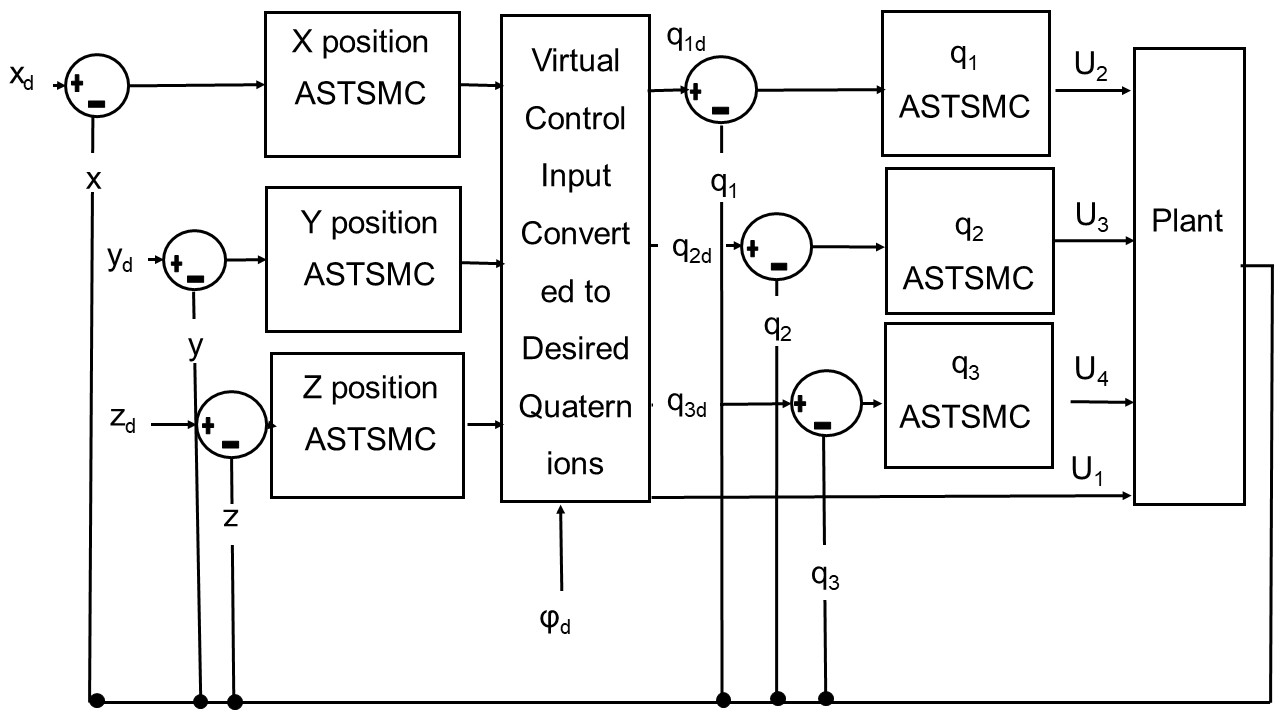
\includegraphics[width=0.65\linewidth]{figures/Fig2.General architecture for UAV quadcopter control.jpg}
    \caption{Controller architecture for quadrotor, including position, altitude, and virtual control input designs}
    %\caption{Controller architecture for quadrotor, including position, altitude, and virtual control input designs\cite{abera2024improved}}
    \label{fig:Controller architecture for quadrotor}
\end{figure}





%\textbf{Design sliding manifold.} The following procedures should be taken to design a sliding manifold.  
  Figure\ref{fig:Controller architecture for quadrotor} shows the general architecture for both position and attitude controller, in this figure desired $x_d,y_d $ and $z_d$ are compared with actual $x,y $ and $z$ then the errors are fed to sliding surface and then a position control law are implemented and results to virtual control inputs which are then combined with desired yaw angle and converted to desired quaternions which then be used as reference to actual quaternion ready for manipulating and obtain roll,pitch and yaw control inputs. It is proposed that firstly a position controller be designed using following steps.
\begin{enumerate}
  \item Determine the quadcopter desired trajectory.
  \begin{equation}
  \begin{bmatrix}
  e_x \\ e_y \\ e_z
  \end{bmatrix}
  =
  \begin{bmatrix}
  x_d - x \\ y_d - y \\ z_d - z
  \end{bmatrix},
  \quad
  \begin{bmatrix}
  \dot{e}_x \\ \dot{e}_y \\ \dot{e}_z
  \end{bmatrix}
  =
  \begin{bmatrix}
  \dot{x}_d - \dot{x} \\ \dot{y}_d - \dot{y} \\ \dot{z}_d - \dot{z}
  \end{bmatrix}
  \label{eqn:surface errors}
  %\tag{4.6}
  \end{equation}

  %\item Design a sliding manifold, a function that measures the difference between the quadcopter actual and desired states. Designing the sliding surface in accordance with the dynamics of the error is the first stage in minimizing the difference between the desired and the actual value, and Stoline and Li proposed the general form of the following equation in~\cite{bouabdallah2004pid}:

  \item Design sliding surfaces
  
 % \begin{equation}
%\sigma = \left( \lambda + \frac{d}{dt} \right)^p e
%\label{eq:sliding_general}
%\tag{4.7}
%\end{equation}


%where $e$ is the tracking error, defined as for z-axis $e(z) = z_d - z$ (the error between the desired trajectory and the actual trajectory in the x-axis); $\lambda$ and $c$ is a positive constant that interprets the dynamics of the surface and $p=n-1$, $n$ is relative degree between output and input. Based on Eq.~\eqref{eq:sliding_general}, position controller sliding manifold can be designed:

\begin{equation}
\begin{cases}
\sigma_x = \lambda_x e_x + c_x \dot{e}_x, \\
\sigma_y = \lambda_y e_y + c_y \dot{e}_y, \\
\sigma_z = \lambda_z e_z + c_z \dot{e}_z
\label{eq:position sliding manifold}
\end{cases}
%\tag{4.8}
\end{equation}
Where  $ \lambda_i $  and   $c_i$  denotes positive position error and velocity error respectively.

\noindent
3. Design control law and tune the gain of sliding surface using PSO.

\subsection*{Design super twisting sliding mode controller}
STSMC is given by the equation below:

\begin{equation}
U_{st} = -\alpha \sqrt{|\sigma|}\,\text{sign}(\sigma) - \nu
\label{eq:supertwisting for x axis}
%\tag{4.9}
\end{equation}

\begin{equation}
\dot{\nu} = \frac{\beta}{2}\,\text{sign}(\sigma)
\label{eq:v_x}
%\tag{4.10}
\end{equation}

The total control law ($U$) calculated by summing the equivalent and supertwisting control law:

\begin{equation}
U = U_{equ} + U_{st}
\label{eq:total control law}
%\tag{4.11}
\end{equation}

where $U_{equ}$ is equivalent controller and $U_{st}$ is super twisting controller. 

Fig.~\ref{fig:position controller smc} illustrates the position controller diagram designed for the quadcopter. The controller focuses on maintaining the desired trajectory by controlling the quadcopter position in the $x$, $y$, and $z$ axes.

After selecting the sliding surface, the next step is to design the equivalent control law, and this law ensures the system remains in sliding mode during operation. Equivalent control law can be designed by making $\dot{\sigma}_x, \dot{\sigma}_y, \dot{\sigma}_z = 0$.

The virtual controller $(U_x, U_y, U_z)$ which means that the three common input will control
motion along x, y and z and these virtual control are given by equation.
\begin{equation}
\left\{
\begin{aligned}
U_x &= \frac{\lambda_x}{c_x}\dot{e}_x + \ddot{x}_d - \alpha_x \sqrt{|\sigma_x|}\, \text{sign}(\sigma_x) - v_x, \\[6pt]
U_y &= \frac{\lambda_y}{c_y}\dot{e}_y + \ddot{y}_d - \alpha_y \sqrt{|\sigma_y|}\, \text{sign}(\sigma_y) - v_y, \\[6pt]
U_z &= \frac{\lambda_z}{c_z}\dot{e}_z + \ddot{z}_d - \alpha_z \sqrt{|\sigma_z|}\, \text{sign}(\sigma_z) - v_z.
\end{aligned}
\right.
\label{eq:virtual control law for position}
%\tag{4.12}
\end{equation}

where $\alpha, \beta$ are the gain of super twisting algorithm and 
$\dot{v} = -\frac{\beta}{2}\text{sign}(\sigma)$.




%\begin{figure}[h!]
   % \centering
   % 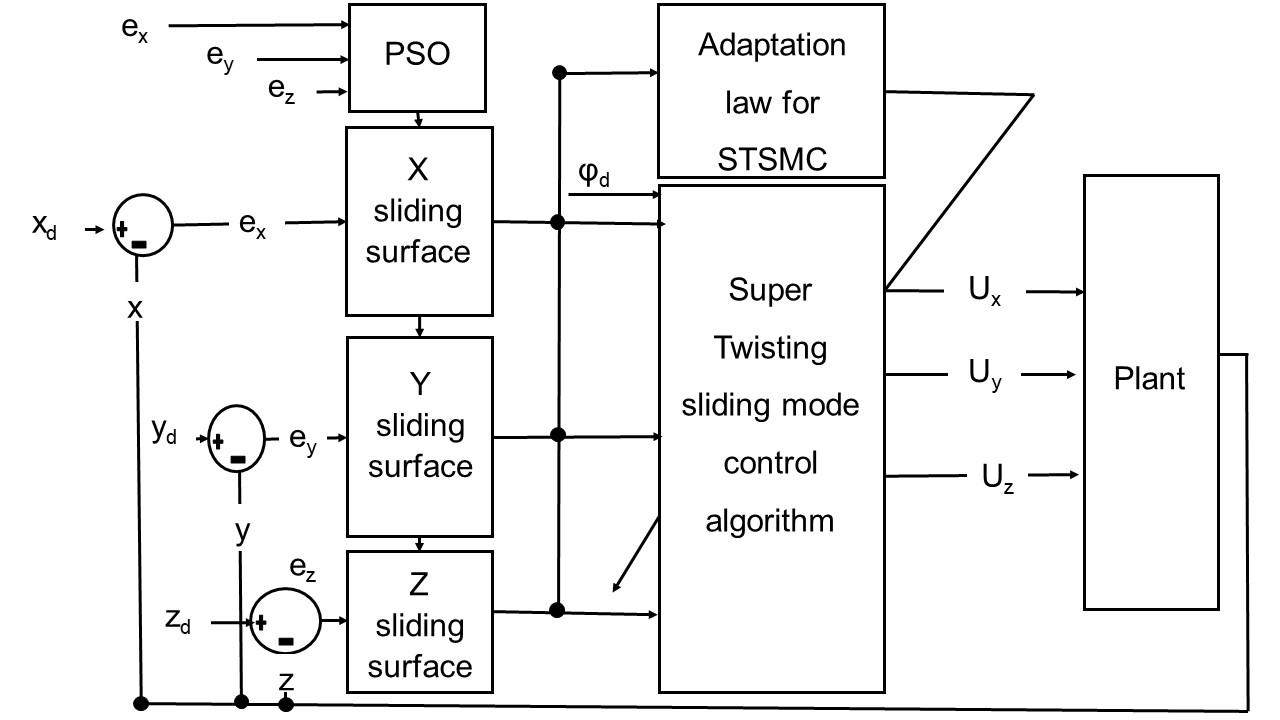
\includegraphics[width=1.0\linewidth]{figures/Fig3.Position Controller for UAV quadcopter - Copy.jpg}
    %\caption{Diagram of position controller for maintaining quadrotor trajectory along x,y,and zaxes}
    %\caption{Diagram of position controller for maintaining quadrotor trajectory along x,y,and zaxes\cite{abera2024improved}}
   % \label{fig:position controller smc}
%\end{figure}

\begin{figure}[h!]
    \centering
    \begin{minipage}{0.48\linewidth}
        \centering
        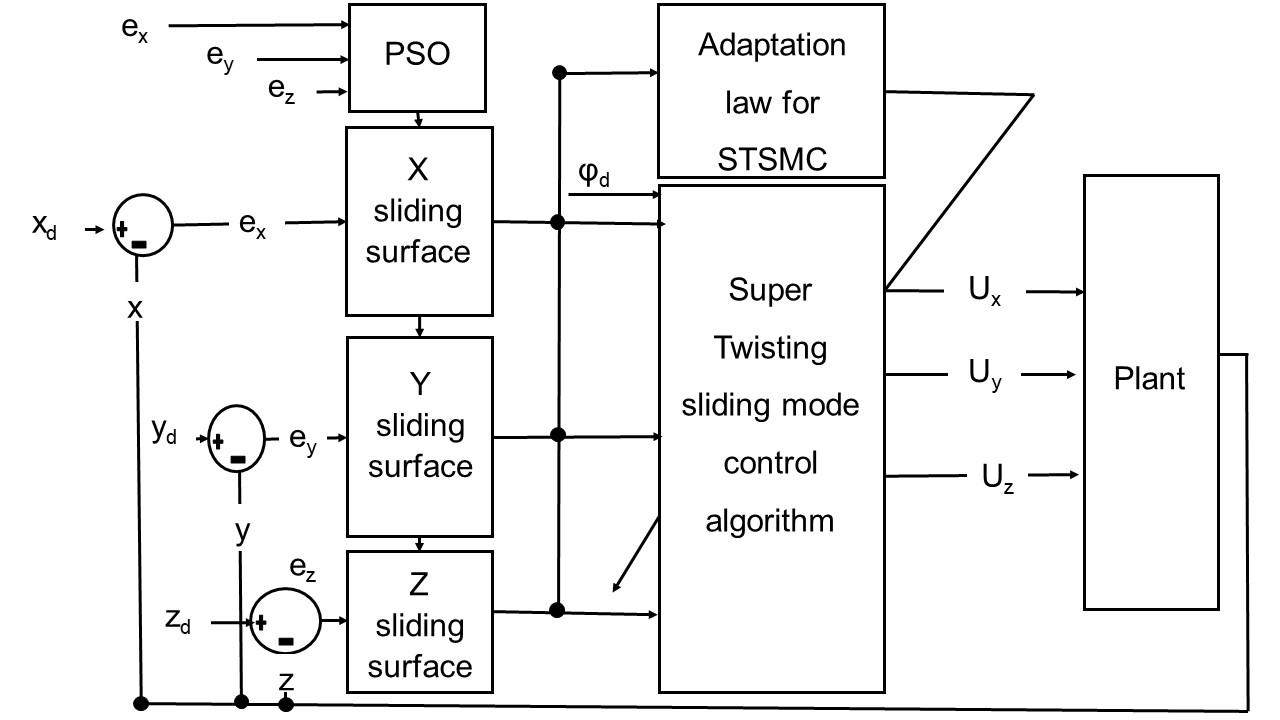
\includegraphics[width=1.0\linewidth]{figures/Fig3.Position Controller for UAV quadcopter - Copy.jpg}
        \caption{Diagram of position controller for maintaining quadrotor trajectory along x,y,and zaxes}
        \label{fig:position controller smc}
    \end{minipage}
    \hfill
    \begin{minipage}{0.48\linewidth}
        \centering
       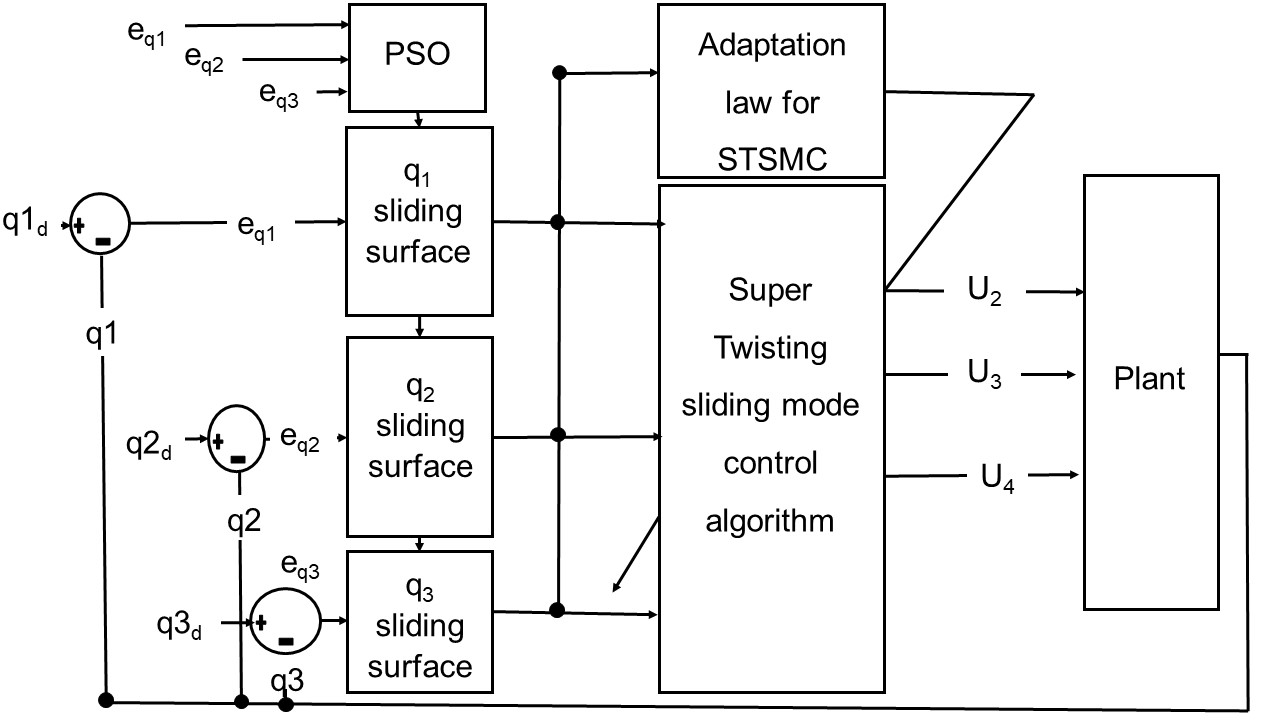
\includegraphics[width=1\linewidth]{figures/Fig4.Attitude Controller for UAV quadcopter.jpg}
    \caption{Altitude controller diagram for maintaining desired quadrotor altitude}
   % \caption{Altitude controller diagram for maintaining desired quadrotor altitude\cite{abera2024improved}}
    \label{fig:attitude controller}
    \end{minipage}
\end{figure}




\begin{theorem}
If the quadrotor position system~\eqref{3.26}, is taken into consideration, together with the
PSO based sliding manifold~\eqref{eq:supertwisting for x axis}, control laws~\eqref{eq:virtual control law for position}, and tracking errors~\eqref{eqn:surface errors}, 
asymptotically, the closed loop tracking error can approach zero. 

The control law must ensure that $\dot{V}(z) < 0$ and the system state variables $V(z) > 0$.
\end{theorem}

\noindent \textbf{Proof.} 
Lyapunov function is a positive scalar function, defined as
\begin{equation}
    V_z = \tfrac{1}{2} \sigma^T \sigma = \tfrac{1}{2} \sigma^2 \sigma.
\end{equation}


Now differentiating $V_z$ with respect to time it was found to be:

%The control law must ensure that $\dot{V}(z) < 0$ and the system state variables $V(z) > 0$.
\begin{equation}
\begin{align*}
\dot{V}_z &= \sigma_z \dot{\sigma}_z < 0  = \sigma_z \big(\lambda_z \dot{e}_z + c_z (\ddot{z}_d - \ddot{z})\big)\\[6pt]
%\dot{V}_z &= \sigma_z \big(\lambda_z \dot{e}_z + c_z (\ddot{z}_d - \ddot{z})\big)
\end{align*}  
\end{equation}


To substitute the value of $\ddot{z}$, use the virtual control law.
\begin{equation}
\begin{align*}
&= \lambda_z \dot{e}_z + c_z \Big(\ddot{z}_d - \alpha_z \sqrt{|\sigma_z|}\,\text{sign}(\sigma_z) 
   - \int \beta_z \,\text{sign}(\sigma_z)\, dt \Big)
\end{align*}
\end{equation}

\begin{equation}
\begin{align}
\dot{V}_z &= \sigma_z \Big(\lambda_z \dot{e}_z + c_z \ddot{z}_d - \lambda_z \dot{e}_z 
   - c_z \ddot{z}_d - \alpha_z \sqrt{|\sigma_z|}\,\text{sign}(\sigma_z) 
   - \int \beta_z \,\text{sign}(\sigma_z)\, dt \Big) \label{4.14} %\tag{4.13}
\end{align}
\end{equation}
\begin{equation}
\begin{align*}
\dot{V}_z &= \sigma_z \Big(-\alpha_z \sqrt{|\sigma_z|}\,\text{sign}(\sigma_z) 
   - \int \beta_z \,\text{sign}(\sigma_z)\, dt \Big) \leq 0
\end{align*}
\end{equation}
To make the Lyapunov function valid, the gains $\alpha_z, \beta_z$ should be above positive.


The virtual control in Eq.~\ref{eq:virtual control law for position}, used to determine desired quaternion value. 
When $x, y,$ and $z$ approach $x_d, y_d,$ and $z_d$ as time reaches the sliding surface 
$\sigma_x = 0, \; \sigma_y = 0, \; \sigma_z = 0$ and the designed controller derives the actual value 
to the desired position. The desired quaternion value can also be calculated by rearranging 
the virtual control inputs.


%\begin{subequations}
%\begin{align}
%U_1 &= \sqrt{U_x^2 + U_y^2 + (U_z + mg)^2} \tag{4.14} \\[8pt]
%q_{0d} &= \tfrac{1}{2}\sqrt{\frac{U_z + mg}{U_1} - 2\sin^2(\psi_d/2) + 1} \tag{4.15} \\[10pt]
%q_{1d} &= \sin(\psi_d/2)U_x + \tfrac{1}{\sqrt{2}}U_y
         % \sqrt{\frac{U_z + mg}{U_1} - 2\sin^2(\psi_d/2) + 1} \tag{4.16} \\[12pt]
%q_{2d} &= \frac{\sin(\psi_d/2)U_y - \tfrac{1}{\sqrt{2}}U_x
         % \sqrt{\frac{U_z + mg}{U_1} - 2\sin^2(\psi_d/2) + 1}}
         % {U_z + mg + U_1} \tag{4.17} \\[12pt]
%q_{3d} &= \sin\!\left(\tfrac{\psi_d}{2}\right) %\tag{4.18}
%\end{align}
%\end{subequations}

\begin{equation}
U_1 = \sqrt{U_x^2 + U_y^2 + (U_z + mg)^2}
%\tag{35}
\label{eq:35}
\end{equation}

\begin{equation}
\left\{
\begin{aligned}
q_{0d} &= \tfrac{1}{2} \sqrt{\frac{U_z + mg}{U_1} - 2\sin^2\!\left(\tfrac{\psi_d}{2}\right) + 1}, \\[8pt]
q_{1d} &= \sin\!\left(\tfrac{\psi_d}{2}\right) U_x 
+ \tfrac{1}{\sqrt{2}} U_y \sqrt{\frac{U_z + mg}{U_1} - 2\sin^2\!\left(\tfrac{\psi_d}{2}\right) + 1}, \\[8pt]
q_{2d} &= \frac{ \sin\!\left(\tfrac{\psi_d}{2}\right) U_y 
- \tfrac{1}{\sqrt{2}} U_x \sqrt{\frac{U_z + mg}{U_1} - 2\sin^2\!\left(\tfrac{\psi_d}{2}\right) + 1} }
{U_z + mg + U_1}, \\[8pt]
q_{3d} &= \sin\!\left(\tfrac{\psi_d}{2}\right).
\end{aligned}
\right.
%\tag{36}
\label{eq:36}
\end{equation}

\subsection{Attitude controller design}
\noindent
\textbf{Fig~\ref{fig:attitude controller}}, depicts the altitude controller diagram responsible for maintaining the quadcopter desired altitude. The controller operates by generating control input signals based on the reference inputs provided by the conversion blocks.
%\begin{figure}[h!]
  %  \centering
    %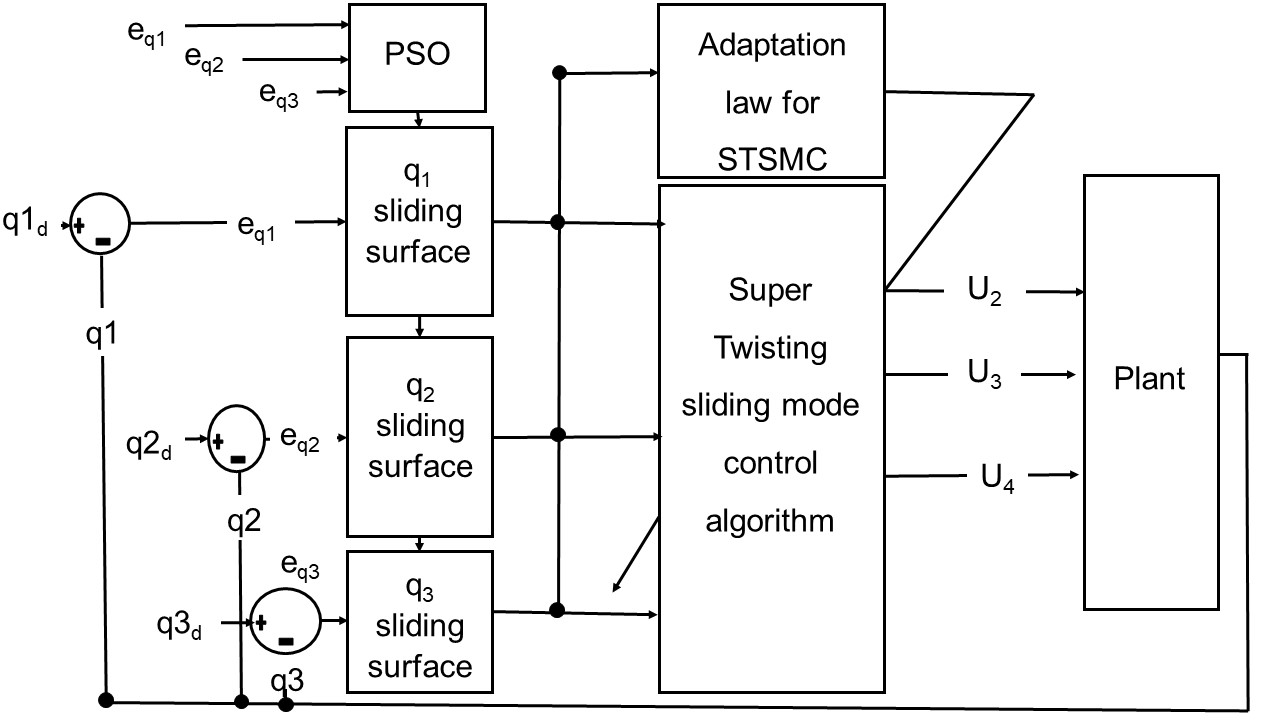
\includegraphics[width=1\linewidth]{figures/Fig4.Attitude Controller for UAV quadcopter.jpg}
   % \caption{Altitude controller diagram for maintaining desired quadrotor altitude}
   % \caption{Altitude controller diagram for maintaining desired quadrotor altitude\cite{abera2024improved}}
   % \label{fig:attitude controller}
%\end{figure}

By generating the input control signal $(U_2, U_3, U_4)$, the adaptive super twisting sliding 
mode control maintains the tracking errors of the attitude subsystem. 
The tracking errors are defined:
\begin{equation}
\begin{bmatrix}
e_{q_1} \\[6pt]
e_{q_2} \\[6pt]
e_{q_3}
\end{bmatrix}
=
\begin{bmatrix}
q_{1d} - q_1 \\[6pt]
q_{2d} - q_2 \\[6pt]
q_{3d} - q_3
\end{bmatrix}
\label{eq:attitude for error}
%\tag{4.20}
\end{equation}

Like position control design, to design altitude controller first step is designing of sliding surface:
\begin{equation}
\left\{
\begin{aligned}
\sigma_{q_1} &= \lambda_{q_1} e_{q_1} + c_{q_1}\dot{e}_{q_1} \\[6pt]
\sigma_{q_2} &= \lambda_{q_2} e_{q_2} + c_{q_2}\dot{e}_{q_2} \\[6pt]
\sigma_{q_3} &= \lambda_{q_3} e_{q_3} + c_{q_3}\dot{e}_{q_3}
\end{aligned}
\right.
\label{eq:sliding surfaces for attitude}
%\tag{4.21}
\end{equation}


\noindent\textbf{Theorem 2.} If the quadrotor attitude system , is designed with 
PSO-based sliding ~\eqref{3.26}surfaces~\eqref{eq:sliding surfaces for attitude}, the closed loop system’s tracking errors~\eqref{eq:attitude for error}, 
can asymptotically converge to zero.  

\noindent Proof. The Lyapunov function is stated as 
$V_{q_1} = \tfrac{1}{2}\sigma_{q_1}^T \sigma_{q_1}$, with $V(q_1) > 0$ and the control law 
requiring $\dot{V}(q_1) < 0$.  
\begin{equation}
\left\{
\begin{align}
V_{q_1} &= \tfrac{1}{2}\sigma_{q_1}^T \sigma_{q_1} \\[6pt]
\dot{V}_{q_1} &= \sigma_{q_1}\dot{\sigma}_{q_1} \leq 0 \\[6pt]
\dot{V}_{q_1} &= \sigma_{q_1}\big(\lambda_{q_1} e_{q_1} + c_{q_1}(\ddot{q}_{1d}-\ddot{q}_1)\big) \\[6pt]
\dot{V}_{q_1} &= \sigma_{q_1}\Bigg(\lambda_{q_1} e_{q_1} + c_{q_1}\dot{q}_{1d} 
   - c_{q_1}\Big(\frac{J_{yy}-J_{zz}}{J_{xx}} \dot{q}_1 \dot{q}_3 
   - \frac{J_t}{J_{xx}} \dot{q}_1 \omega \Big)\Bigg) \\[6pt]
U_2 &= J_{xx}\Bigg(\lambda_{q_1} e_{q_1} + \dot{q}_{1d} 
   - \Big(\frac{J_{yy}-J_{zz}}{J_{xx}} \dot{q}_1 \dot{q}_3 
   - \frac{J_t}{J_{xx}} \dot{q}_1 \omega \Big) + U_{st}\Bigg) \\[6pt]
\dot{V}_{q_1} &= \sigma_{q_1}\Big(-\alpha_{q_1}\sqrt{|\sigma_{q_1}|}\,\text{sign}(\sigma_{q_1}) 
   - \int \beta_{q_1}\text{sign}(\sigma_{q_1})dt\Big) \leq 0
\end{align} 
\right.
\end{equation}




\noindent Consequently, the altitude tracking errors will asymptotically approach zero, and the attitude control inputs becomes
%Below are the attitude control inputs
%%%%%%%%%%%%%%
\begin{small}
\begin{equation}
\left\{
%\[
\begin{aligned}
U_2 &= \frac{J_{xx}}{c_{q1}} \left( -2\alpha_{q_1}\sqrt{|\sigma_{q_1}|}\,\text{sign}(\sigma_{q_1}) + \nu_{q_1} - \lambda_{q1} p \right) \\
&\quad - (J_{yy} - J_{zz}) q r + J_p q \Omega_r + C_{ap} p \\[6pt]
U_3 &= \frac{J_{yy}}{c_{q2}} \left( -2\alpha_{q_2}\sqrt{|\sigma_{q_2}|}\,\text{sign}(\sigma_{q_2}) + \nu_{q_2} - \lambda_{q2} q \right) \\
&\quad - (J_{zz} - J_{xx}) p r - J_p p \Omega_r + C_{aq} q \\[6pt]
U_4 &= \frac{J_{zz}}{c_{q3}} \left( -2\alpha_{q_3}\sqrt{|\sigma_{q_3}|}\,\text{sign}(\sigma_{q_3}) + \nu_{q_3} - \lambda_{q3} r \right) \\
&\quad - (J_{xx} - J_{yy}) p q + C_{ar} r
\end{aligned} 
\right.
\end{equation}
\end{small}

\[
\dot{\nu} = -\tfrac{\beta}{2}\text{sign}(\sigma)
\]

%%%%%%%%



%begin{small}

%\[
%\left\{
%\begin{aligned}
%U_2 &= J_{xx}\Bigg[\tfrac{\lambda_{q_1}}{c_{q_1}} e_{q_1} + \ddot{q}_{1d} 
  % - \Big(\tfrac{J_{yy}-J_{zz}}{J_{xx}} \dot{q}_1 \dot{q}_3 
  % - \tfrac{J_t}{J_{xx}} \dot{q}_1 \omega_T \Big)\Bigg] 
 %  - \alpha_{q_1}\sqrt{|\sigma_{q_1}|}\,\text{sign}(\sigma_{q_1}) + \nu_{q_1} \\[8pt]
%U_3 &= J_{yy}\Bigg[\tfrac{\lambda_{q_2}}{c_{q_2}} e_{q_2} + \ddot{q}_{2d} 
 %  - \Big(\tfrac{J_{zz}-J_{xx}}{J_{yy}} \dot{q}_2 \dot{q}_3 
 %  + \tfrac{J_t}{J_{yy}} \dot{q}_2 \omega_T \Big)\Bigg] 
 %  - \alpha_{q_2}\sqrt{|\sigma_{q_2}|}\,\text{sign}(\sigma_{q_2}) + \nu_{q_2} \\[8pt]
%U_4 &= J_{zz}\Bigg[\tfrac{\lambda_{q_3}}{c_{q_3}} e_{q_3} + \ddot{q}_{3d} 
 %  - \Big(\tfrac{J_{xx}-J_{yy}}{J_{zz}} \dot{q}_1 \dot{q}_2 \Big)\Bigg] 
  % - \alpha_{q_3}\sqrt{|\sigma_{q_3}|}\,\text{sign}(\sigma_{q_3}) + \nu_{q_3}
%\end{aligned}
%\right.



\subsection{SMC gain tuning}

The particle swarm approach was developed by the movements of birds and swimming fish, 
the notion for the optimization of nonlinear systems was  further developed in~\cite{blackwell2007particle}. 
PSO is very simple and efficient method to adjust gain for controllers when compared to other optimization techniques~\cite{el2020particle}. In this research, a PSO is chosen to 
automatically adjust the quadcopter altitude and attitude control gain of SMC controller. 
The various parameters that make up this fitness function are taken from trajectory 
monitoring and regulation of the coupled and nonlinear dynamics of a quadcopter. 
Every particle’s position is associated with SMC. Each particle’s speed in the two 
simulations is corresponding to this parametrized change. Every particle and variable has 
its position and velocity initialized at random. Every particle travels across the search 
space, and every particle’s effectiveness is assessed on a regular basis.

The PSO algorithm is computationally efficient, conceptually straightforward, and simple 
to apply. Fig.~\ref{fig:PSO for sliding surface parameters} presents the flowchart of PSO algorithm, which is 
employed to fine-tune the control parameters of the quadcopter sliding surface. 
The PSO algorithm iteratively optimizes the sliding surface gains. The flowchart outlines 
the key steps of the PSO process, from initializing the particles’ positions and velocities 
to evaluating their performance and updating their positions based on the best-performing particles.


%\begin{figure}[h!]
    %\centering
   % \includegraphics[width=1\linewidth]{Files//Figures/Flowchart of PSO algorithm used for tuning quadrotor sliding surface parameters..PNG}
    %\caption{Flowchart of PSO algorithm used for tuning quadrotor sliding surface parameters\cite{abera2024improved}}
   % \label{fig:PSO for sliding surface parameters}
%\end{figure}

\begin{figure}[h!]
    \centering
    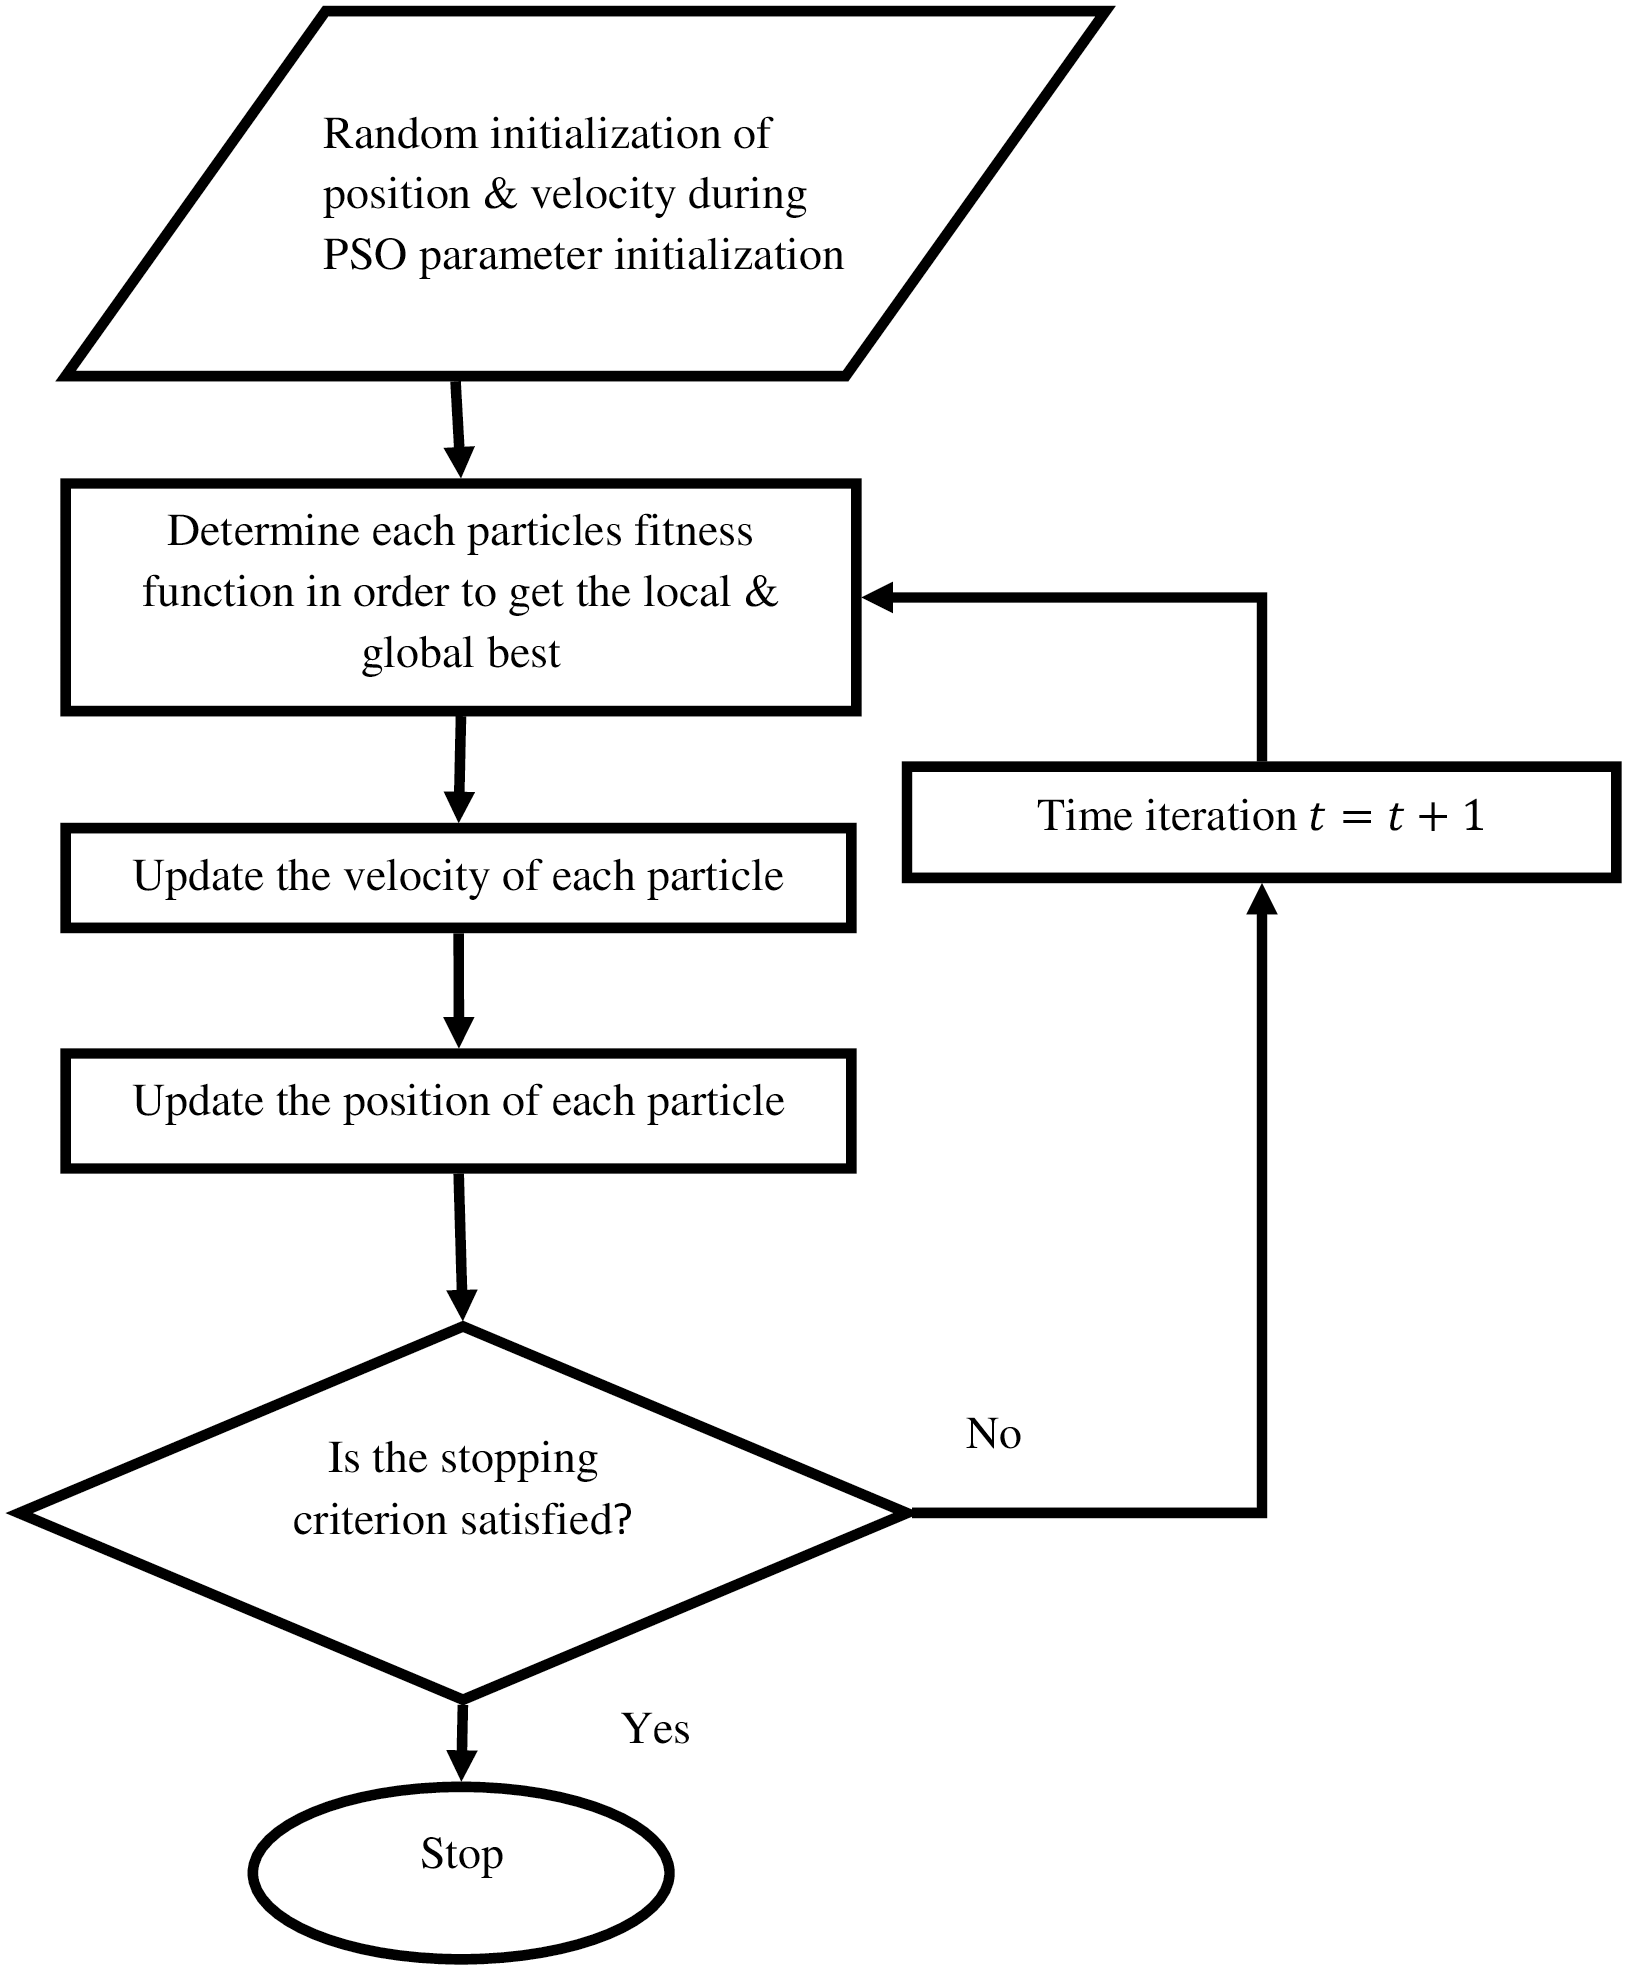
\includegraphics[width=0.5\linewidth]{figures/fig5.Flowchart of PSO algorithm used for tuning quadrotor sliding surface parameters..PNG}

    % Caption for List of Figures (no citation)
    \caption{Flowchart of PSO algorithm used for tuning quadrotor sliding surface parameters} \cite{abera2024improved}

    % Caption shown only under the figure (with citation)
   % \caption*{Source: \cite{abera2024improved}}

    \label{fig:PSO for sliding surface parameters}
\end{figure}

\subsection{Fitness function}


Using the proposed approach, a performance index is used to quantify the optimization 
performance of the quadrotor’s responses. The purpose of the performance index, sometimes 
referred to as the fitness function, is to reduce the differences between the quadrotor’s 
controllable and desired output responses. The goal of this  is to reduce quadcopter 
trajectory tracking error in terms of both position and orientation. Systems constructed 
using Integral Time Absolute Error (ITAE) have minor overshoots and minimal damped 
oscillations. This research utilized the ITAE performance index.

\begin{equation}
ITAE = \int_{0}^{\infty} t |e(t)| \, dt  
\end{equation}


The fittness function used in tunning gains for position controller was as follows:
\begin{equation}
ITAE = \int_{0}^{\infty} t\,\left( |e(x)| + |e(y)| + |e(z)| \right)\, dt
%\tag{4.22}
\label{eq:4.22}
\end{equation}

   The fittness function used in tunning gains for attitude controller was as follows:


\begin{equation}
ITAE = \int_{0}^{\infty} t\,\left( |e(q1)| + |e(q2)| + |e(q3)| \right)\, dt
%\tag{4.23}
\label{eq:4.23}
\end{equation}


Below are the PSO's parameters that were used during tuning for attitude and position controller gains  as shown in Table~\ref{tab:PSO_ITAE_attitude} and Table~\ref{tab:PSO_Position_Gains}.  %


 \small
  \setlength{\arraycolsep}{3pt}  % <-- reduces spacing between columns

  \[
  \mathbf{uba} =
  \left[
  \begin{array}{cccccccccccc}
  100 & 100 & 100 & 100 & 100 & 100 & 100 & 100 & 100 & 100 & 100 & 100
  \end{array}
  \right]
  \]

  \[
  \mathbf{lba} =
  \left[
  \begin{array}{cccccccccccc}
  0 & 0 & 0 & 0 & 0 & 0 & 0 & 0 & 0 & 0 & 0 & 0
  \end{array}
  \right]
  \]

      \[
  \mathbf{ubp} =
  \left[
  \begin{array}{cccccccccccc}
  100 & 100
  \end{array}
  \right]
  \]

  \[
  \mathbf{lbp} =
  \left[
  \begin{array}{cccccccccccc}
  0 & 0 
  \end{array}
  \right]
  \]

  }%
}


  \[
  v_{\max} = 1,\quad
  v_{\min} = 0.1,\quad
  c_{1}=2,\quad
  c_{2}=2
  \]



\[
\textit{Note:}\;
\begin{aligned}
uba      &= \text{upper attitude bound}, \\
lba      &= \text{lower attitude bound}, \\
ubp      &= \text{upper position bound}, \\
lbp     &= \text{lower position bound}, \\
v_{\max} &= \text{maximum particle swarm velocity coefficient}, \\
v_{\min} &= \text{minimum particle swarm velocity coefficient}, \\
c_{1}    &= \text{first particle swarm acceleration coefficient}, \\
c_{2}    &= \text{second particle swarm acceleration coefficient}.
\end{aligned}
\]











\subsection{Adaptive super twisting sliding mode control design}


\textbf{Control structure of adaptive super twisting sliding mode control.} 
After that, super twisting control is considered

\begin{align*}
U_{st} &= -\alpha |\sigma|^{\tfrac{1}{2}} \, \text{sign}(\sigma) + \nu \\[6pt]
\dot{\nu} &= -\tfrac{\beta}{2}\text{sign}(\sigma)
\end{align*}

The adaptive gains are stated as follows:
\begin{align}
\alpha &= \alpha(\sigma, \dot{\sigma}, t) 
\label{4.24} \\[6pt]
\beta &= \beta(\sigma, \dot{\sigma}, t) \label{4.25}
\end{align}

\textbf{Lemma 1.} The adaptation law are to be defined as:

\begin{align}
\dot{\alpha} &=
\begin{cases}
\omega_1 \tfrac{\sqrt{\gamma_1}}{\sqrt{2}} \, \text{sign}(|\sigma|-\mu), & \text{if } \alpha > \alpha_m \\[6pt]
\eta, & \text{if } \alpha \leq \alpha_m
\end{cases} \label{4.26}
\end{align}

\begin{align*}
\beta &= 2 \epsilon \alpha
\end{align*}



The parameters $\epsilon, \gamma_1, \omega, \eta$ are arbitrary positive constants, 
while $\alpha_m$ is a small positive constant.  

\noindent \textbf{Proof.} Lyapunov function candidate is introduced as:
\begin{align}
\nu(\alpha,\beta) = \nu_0 + \tfrac{1}{2\gamma_1}(\alpha-\alpha^*)^2 + \tfrac{1}{2\gamma_2}(\beta-\beta^*)^2 \label{4.27}
\end{align}

where $\nu_0$ is Lyapunov function for $(\sigma,\dot{\sigma})$, 
$\alpha^*, \beta^*$ are maximum possible values of $\alpha, \beta$.



respectively. The derivative of the Lyapunov function is as follows:
\begin{align}
\dot{\nu}(\sigma,\alpha,\beta) &\leq -\eta_0 \sqrt{\nu(\sigma,\alpha,\beta)} 
- |\epsilon_\alpha|\left(\tfrac{1}{\gamma_1}\dot{\alpha} - \tfrac{\omega_1}{\sqrt{2\gamma_1}}\right) \notag \\[6pt]
&\quad - |\epsilon_\beta|\left(\tfrac{1}{\gamma_2}\dot{\beta} - \tfrac{\omega_2}{\sqrt{2\gamma_2}}\right) \label{4.28}
\end{align}

It gives
\begin{align}
\dot{\nu}(\sigma,\alpha,\beta) \leq -\eta_0 \sqrt{\nu(\sigma,\alpha,\beta)} + \zeta \label{4.29}
\end{align}

with
\begin{align}
\zeta &= -|\epsilon_\alpha|\left(\tfrac{1}{\gamma_1}\dot{\alpha} - \tfrac{\omega_1}{\sqrt{2\gamma_1}}\right) 
        - |\epsilon_\beta|\left(\tfrac{1}{\gamma_2}\dot{\beta} - \tfrac{\omega_2}{\sqrt{2\gamma_2}}\right) \label{4.30}
\end{align}

where $\epsilon_\alpha = \alpha - \alpha^*$ and $\epsilon_\beta = \beta - \beta^*$. 
It is evident that the system’s finite-time convergence is assured 
\cite{besnard2007control}.


\begin{table}[htbp]
\centering

\caption[Plant parameter]{Plant parameter.  \cite{bresciani2008modelling}}
\label{tab:Plant parameter for simulation}

\resizebox{\linewidth}{!}{%
\begin{tabular}{|c|c|c|c|}
\hline
\textbf{Plant Parameters} & \textbf{Symbol} & \textbf{Unit} & \textbf{Values} \\ \hline
Thrust coefficient & $b$ & $Ns^2$ & $54.2 \times 10^{-6}$ \\ \hline
Drag factor & $d$ & $Nms^2$ & $1.1 \times 10^{-6}$ \\ \hline
Gravitational Acceleration & $g$ & $m/s^2$ & $9.81$ \\ \hline
The length of the arm of the quadrotor & $\l$ & $m$ & $0.24$ \\ \hline
Mass of quadrotor & $m$ & $Kg$ & $1$ \\ \hline
Inertia around X-axis & $J_{xx}$ & $Nms^2$ & $8.1 \times 10^{-3}$ \\ \hline
Inertia around Y-axis & $J_{yy}$ & $Nms^2$ & $8.1 \times 10^{-3}$ \\ \hline
Inertia around Z-axis & $J_{zz}$ & $Nms^2$ & $14.23 \times 10^{-3}$ \\\hline
%\hline

\end{tabular}
}
\end{table}

Table~\ref{tab:Plant parameter for simulation},  presents different  parameters of quadrotor and Tables~\ref{tab:Design parameter for ASTSMC.}--\ref{tab:Design parameter of adaptation law.}, give the design parameters of the controller,note that values written in Tables ~\ref{tab:Design parameter for ASTSMC.} and \ref{tab:Design parameter for PSO SMC.} were obtained after running a PSO algorithm where as parameters in Table \ref{tab:Design parameter of adaptation law.} were adopted from article \cite{abera2024improved}.  

\textbf{Remark 1.}  In order to achieve best trajectory tracking optimal gain was  obtained using PSO technique.

%Simulation results for optimal STSMC that is adaptive are presented here in where as mathematical model used captures some of the dynamics ignored in most of currennt literatures.


\begin{table}[h!]
\centering
\caption{Design parameter for PSO SMC.}
\begin{tabular}{|l|c|}
\hline
\textbf{Parameter} & \textbf{Value} \\ \hline
$\lambda_x,$\lambda_y,$\lambda_z, & 80,80,80 \\ \hline

 $ \lambda_{q_1},  \lambda_{q_2}$   \lambda_{q_3}& 100,83.4608,100 \\ \hline
$c_z, c_z, c_z$ & 1,1,1 \\ \hline
$ c_{q_1}, c_{q_2}, c_{q_3}$ & 0.2351,68.7297,32.0515 \\ \hline

\end{tabular}
\label{tab:Design parameter for PSO SMC.}
\end{table}




\begin{table}[h!]
\centering
\begin{minipage}{0.48\linewidth}
\centering
\caption{Design parameters for ASTSMC}
\label{tab:astsmc_params}
\begin{tabular}{|l|c|}
\hline
\textbf{Parameter} & \textbf{Value} \\ \hline
$a_x,a_y,a_z$ & 0.01, 0.01, 0.01 \\ \hline
$a_{q1},a_{q2},a_{q3}$ & 43.4506, 34.2058, 51.4594 \\ \hline
$\beta_x,\beta_y,\beta_z$ & 0.0002, 0.0002, 0.0002 \\ \hline
$\beta_{q1},\beta_{q2},\beta_{q3}$ & 100, 0, 0.0426 \\ \hline
\end{tabular}
\label{tab:Design parameter for ASTSMC.}
\end{minipage}
\hfill
\begin{minipage}{0.48\linewidth}
\centering
\caption{Design parameters of adaptation law}
\label{tab:adapt_params}
\begin{tabular}{|l|c|}
\hline
\textbf{Parameter} & \textbf{Value} \\ \hline
$\omega_1$ & 0.0001 \\ \hline
$a_m$ & 0.01 \\ \hline
$\eta$ & 0.01 \\ \hline
$\gamma_1$ & 2 \\ \hline
$\mu$ & 0.7 \\ \hline
\end{tabular}
\label{tab:Design parameter of adaptation law.}
\end{minipage}
\end{table}

\section{Experimental Validation}

\begin{table}[h]
\centering
\caption{Hardware components used in the quadrotor system}
\label{tab:hardware}
\begin{tabular}{|c|l|l|}
\hline
S/No & Item & Specs \\ 
\hline
01 & Teensy & 4.0 \\ 
02 & MPU6050 & GY-521 \\ 
03 & Spacer & M3 $\times$ 25mm \\ 
04 & Battery & 3S / 11.1V 460mAh \\ 
05 & Emax ESC & BLHeli-12A \\ 
06 & Brushless motor & ECO 1106-4500KV \\ 
07 & Battery Connector & XT60 \\ 
08 & RC transmitter & FS-I6X \\ 
09 & Receiver FS-IA6B & PWM 6CH 2.4GHz \\ 
10 & Power switch & BTS50055-1TMB \\ 
11 & Resistor & 100$\Omega$, 510$\Omega$, 2000$\Omega$ \\ 
12 & Zener Diode & BZX55C2V4 \\ 
13 & Female to Female Jumper wires & -- \\ 
14 & LEDs & Red and Green -- 5V \\ 
15 & Lower and Upper frame & CarbonAeronautics \\ 
16 & USB & A to Micro B \\ 
17 & Slide switch & OS102011MS2QN1C \\ 
18 & Gemfam propeller & 2218 3-blades \\ 
\hline
\end{tabular}
\end{table}

\subsection*{A. Hardware Architecture}

The hardware architecture of the custom quadcopter platform was composed of a modular embedded control system, sensing units, power electronics, propulsion components, and a lightweight mechanical structure as shown in ``Table\ref{tab:hardware}. The Teensy 4.0 microcontroller was used as the main flight controller and executed the attitude control algorithms while handling communication with onboard sensors, actuators, and the radio receiver. It was mounted at the center of the airframe using M3 $\times$ 25 mm spacers to provide mechanical stability and reduce vibration transmission.

Attitude sensing was achieved using an GY-521 MPU6050 inertial measurement unit, which provided angular rate and acceleration measurements. The IMU was interfaced with the Teensy via the I$^2$C communication bus and was positioned close to the quadcopter’s center of mass to improve measurement accuracy. Signal conditioning and voltage protection were implemented using resistors (100~$\Omega$, 510~$\Omega$, and 2~k$\Omega$) and a BZX55C2V4 Zener diode to ensure reliable operation of the embedded electronics.

The propulsion system consisted of four ECO 1106--4500 KV brushless DC motors, each driven by an EMAX BLHeli-12A electronic speed controller (ESC). The ESCs received pulse-width modulation (PWM) control signals from the Teensy and regulated the motor speeds accordingly. Gemfan 2218 three-blade propellers were mounted on the motors to generate the thrust and control torques required for quadcopter stabilization and maneuvering.

Electrical power was supplied by a 3S (11.1~V), 460~mAh LiPo battery, which was connected through an XT60 battery connector to support the high current demands of the propulsion system. A BTS50055-1TMB power switch and a slide switch (OS102011MS2QN1C) were integrated into the power distribution line to enable safe and controlled power management. System status indications, including power availability and alarming state, were provided using 5~V red and green LEDs.

Pilot commands were transmitted using an FS-I6X radio transmitter and received by an FS-IA6B 6-channel PWM receiver, which was directly interfaced with the Teensy input pins. This configuration allowed real-time manual command input while maintaining compatibility with onboard control algorithms. Female-to-female jumper wires were used for signal routing between components during assembly and testing.

The mechanical structure was formed using upper and lower Carbon Aeronautics frames. which provided a rigid and lightweight airframe suitable for experimental flight tests. 
A USB Type-A to Micro-B cable was used for firmware upload, debugging, and data logging during ground-based experiments. 
The complete assembly is shown in Fig.\ref{fig:quadcopter_setup}.

%\begin{figure}
   % \centering
   % 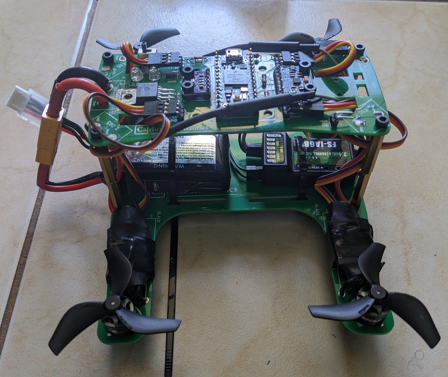
\includegraphics[width=1\linewidth]{figures/assembled Quadcopter.png}
    %\caption{Custom  Assembled Quadcopter}
   % \label{fig:Custom  Assembled Quadcopter}
%\end{figure}

%\begin{figure}
  %  \centering
   % 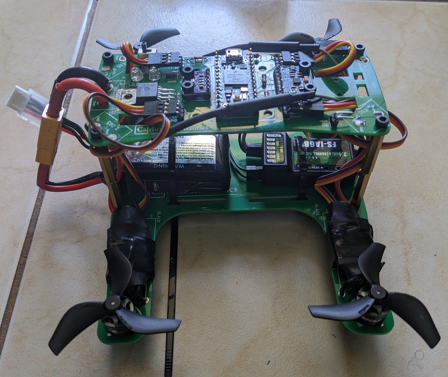
\includegraphics[width=1\linewidth]{figures/assembled Quadcopter.png}
   % \caption{Assembled Quadcopter Mounted on custom UAV test rig ready for experiments.}
   % \label{fig: Assembled Quadcopter on testrig}
%\end{figure}


%%%%%%%%%%%%%%%%%
\begin{figure}[htbp]
    \centering
    
    \begin{subfigure}{0.48\textwidth}
        \centering
        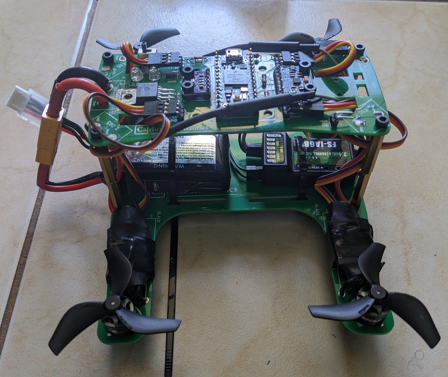
\includegraphics[width=\linewidth]{figures/assembled Quadcopter.png}
        \caption{Custom assembled quadcopter}
        \label{fig:assembled_quadcopter}
    \end{subfigure}
    \hfill
    \begin{subfigure}{0.48\textwidth}
        \centering
        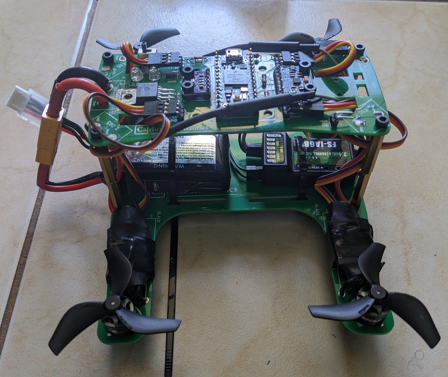
\includegraphics[width=\linewidth]{figures/assembled Quadcopter.png}
        \caption{Quadcopter mounted on custom UAV test rig}
        \label{fig:quadcopter_testrig}
    \end{subfigure}
    
    \caption{Experimental quadcopter platform and test setup}
    \label{fig:quadcopter_setup}
\end{figure}



\subsection*{B.	Sensor Processing}
Sensor processing was implemented to obtain reliable attitude-related measurements required for real-time control of the custom quadcopter. The primary sensing unit used in the platform was the MPU6050 6-DOF inertial measurement unit, which provided three-axis angular velocity and three-axis linear acceleration data. These measurements were used to estimate the quadcopter's attitude and angular rates during flight.

Gyroscope data were sampled at a fixed rate synchronized with the control loop execution. Prior to flight, a gyroscope calibration procedure was performed while the quadcopter was kept stationary. During this process, multiple samples were collected and averaged to estimate constant bias offsets for each axis. These offsets were then subtracted from subsequent gyroscope measurements to reduce steady-state drift.

To mitigate the effects of high-frequency noise caused by motor vibrations and structural resonances, the raw gyroscope signals were processed using a digital low-pass filter. This filtering step improved measurement smoothness while preserving the dynamic response required for attitude control. Accelerometer data were also filtered and normalized to provide a reference for gravity direction, which was essential for correcting long-term drift in orientation estimation.

Attitude estimation was achieved by combining gyroscope and accelerometer measurements using a lightweight sensor fusion algorithm suitable for real-time embedded implementation. The algorithm updated the orientation representation at each control cycle and provided roll, pitch, and yaw information required for feedback control. The chosen approach was computationally efficient and compatible with the limited latency requirements of the embedded system.

All sensor processing operations were executed onboard the Teensy 4.0 microcontroller using floating-point arithmetic. The processed angular rates and attitude estimates were made available to the control algorithm at each control step, ensuring consistent and time-aligned feedback. This sensor processing framework provided accurate and robust attitude information, enabling stable flight and reliable experimental validation of the proposed control strategy.

\subsection*{C.Control Law}

The attitude control of the quadcopter was achieved using an Adaptive Super-Twisting Sliding Mode Controller (ASTSMC). The controller was designed to regulate the quadcopter's rotational dynamics about the roll, pitch, and yaw axes in the presence of model uncertainties, external disturbances, and actuator nonlinearities. This approach was selected to overcome the limitations of conventional PID controllers, particularly their sensitivity to disturbances and parameter variations.

The control design was formulated in the angular-rate domain. For each rotational axis, a sliding surface was defined using a combination of the tracking error and its derivative. The sliding surface represented the desired dynamic behavior of the closed-loop system and served as the basis for control action generation. By enforcing convergence of the sliding surfaces to zero, accurate attitude stabilization was achieved.

To reduce the chattering effect commonly associated with first-order sliding mode control, the super-twisting algorithm was employed. This higher-order sliding mode technique generated a continuous control signal while ensuring finite-time convergence of the sliding variables. As a result, smooth actuator commands were obtained without sacrificing robustness.

An adaptive mechanism was incorporated into the control law to update the sliding surface gains online. These gains were adjusted based on the magnitude of the sliding variables, allowing the controller to automatically increase robustness under high disturbances and reduce control effort during steady-state operation. This adaptive feature improved tracking performance and enhanced stability across different flight conditions.

The control law was implemented in discrete time and executed at a fixed sampling period on the Teensy 4.0 microcontroller. The controller outputs were mapped to pulse-width modulation (PWM) signals, which were sent to the electronic speed controllers to regulate motor speeds. Control saturation limits were applied to ensure safe operation within actuator constraints.

\subsection*{Embedded Implementation}

The controller was implemented in C++ using the Arduino Teensyduino environment. Floating-point arithmetic and interrupt-driven timing ensured deterministic execution.


\clearpage


\chapter{ RESULTS AND DISCUSSION}

%\section{Introduction}

This section presents the results and discussion of the proposed control framework, beginning with model verification to establish the accuracy and reliability of the developed quadrotor dynamics. The verified model provides a sound basis for controller design and performance evaluation. Subsequently, the effectiveness of the Particle Swarm Optimization (PSO) approach in tuning controller parameters is demonstrated, highlighting improvements in convergence and robustness. Finally, trajectory tracking results are analyzed to assess the controller’s ability to achieve precise and stable motion under varying conditions. Together, these results provide a comprehensive validation of the proposed method and its practical applicability.

\section{Verification of Quadrotor Dynamic Model}

%This step in the process of designing control system is also known as Quantitative analyses of the derived model of the system. To verify feasibility of the derived mathematical model of Quadrotor dynamics, simulations were conducted under MATLAB\textsuperscript{\textregistered} Simulink software by using parameter values presented in Table~\ref{tab:quad_params}

%This stage of control system design is referred to as \textit{quantitative analysis} of the derived model. 
To verify the feasibility of the quadrotor dynamic model, simulations were performed in 
MATLAB\textsuperscript{\textregistered} Simulink using the parameter values listed in Table~\ref{tab:quad_params}.


\begin{table}[h!]
\centering
\caption{Specifications for the Quadrotor model design ~\cite{ahmed2018sliding},\cite{bernard2017dynamic}}
\label{tab:quad_params}
\begin{tabular}{|c|l|c|c|}
\hline
\textbf{Symbol} & \textbf{Description} & \textbf{Unit} & \textbf{Value} \\ \hline
$g$     & Acceleration due to gravity              & $ms^{-2}$  & 9.81 \\ \hline
$m$     & Mass of Quadrotor                        & $Kg$       & 0.468 \\ \hline
$J_{xx}$ & Body moment of inertia around the X-axis & $Nms^2$    & $4.856 \times 10^{-3}$ \\ \hline
$J_{yy}$ & Body moment of inertia around the Y-axis & $Nms^2$    & $4.856 \times 10^{-3}$ \\ \hline
$J_{zz}$ & Body moment of inertia around the Z-axis & $Nms^2$    & $8.801 \times 10^{-3}$ \\ \hline
$\ell$   & Length of Quadrotor arm                 & m          & 0.225 \\ \hline
$b$     & Thrust coefficient                       & N/m/s      & $2.98 \times 10^{-6}$ \\ \hline
$d$     & Drag factor                              & $Nms^2$    & $1.140 \times 10^{-7}$ \\ \hline
$J_p$   & Rotor or propeller inertia               & $Nms^2$    & $3.357 \times 10^{-5}$ \\ \hline
$C_{\alpha} = C_{aq} = C_{ar}$ & Rotational drag coefficients & N/m/s & 0.25 \\ \hline
$C_{\alpha} = C_{av} = C_{az}$ & Translational drag coefficients & N/m/s & 0.2 \\ \hline
$R$     & Rotor or propeller Radius                & m          & 0.25 \\ \hline
$\gamma$& Correction factor                        & unit       & 0.083 \\ \hline
\end{tabular}
\end{table}

The open-loop system is analyzed by applying arbitrary inputs based on the following 
flight scenarios:

\begin{itemize}
  \item \textbf{Ascending or descending flight} is controlled by the total thrust $U_1$. 
  If $U_1 > mg$, the quadrotor ascends; if $U_1 < mg$, it descends; and if $U_1 = mg$, 
  it hovers at a constant altitude. In this case, all rotors spin at the same speed, 
  preventing rotational motion.

  \item \textbf{Lateral maneuvering} is achieved through roll and pitch torques 
  $U_2$ and $U_3$. According to Figure~\ref{fig:Quadrotor free body diagram}, if $U_2>0$, 
  the quadrotor rolls along the positive $y$-axis by increasing the speeds of rotors 1 
  and 4 while decreasing those of rotors 2 and 3. Similarly, if $U_3>0$, pitch motion 
  occurs along the negative $x$-axis by increasing the speeds of rotors 1 and 2 and 
  reducing those of rotors 3 and 4.

  \item \textbf{Heading control} is obtained by the yaw torque $U_4$. If $U_4>0$, the 
  quadrotor rotates clockwise about its center of gravity, increasing the speeds of 
  rotors 2 and 4 while decreasing those of rotors 1 and 3 to maintain altitude.
\end{itemize}

In this subsection, the quadrotor model is verified by applying open-loop control inputs. 
First, the vehicle ascends and then hovers at a specified altitude. From this hovering 
condition, roll, pitch, and yaw inputs are applied and MATLAB\textsuperscript{\textregistered} 
Simulink simulations are performed using the parameters listed in Table~\ref{tab:quad_params}.

\begin{itemize}
  \item The weight of the quadrotor is 
  $W = mg = 0.468 \times 9.81 = 4.591\,N$.
\end{itemize}

%\textbf{Ascending maneuver:} In the first scenario, the total thrust is set to 
%$U_1 = 4.7\,N$, which is greater than the gravitational force. As a result, the quadrotor ascends. All propellers rotate at the same speed, producing equal thrust, and therefore no rotational motion or lateral maneuvering along the $x$ or $y$ directions occurs, as illustrated in Figure~\ref{fig:Quad position and ground effect-ascending}.

\textbf{Ascending maneuver:} In the first scenario, the total thrust is set to 
$U_1 = 4.7\,N$ 

The ascending maneuver as shown in Figure~\ref{fig:Quad position and ground effect-ascending} provides a reliable benchmark for validating the proposed quadrotor model. When the applied thrust exceeds gravitational force, a smooth vertical rise is observed, with negligible lateral displacement, confirming stable position behavior along the \(z\)-axis. Both models capture this trend; however, the baseline model predicts a faster altitude increase, while the proposed model shows a more gradual ascent due to aerodynamic drag effects. The propeller speeds remain equal and converge to steady values, indicating balanced thrust generation across all rotors. Furthermore, the Euler angles (roll, pitch, and yaw) remain close to zero throughout the maneuver, confirming the absence of rotational motion and validating symmetry in the system. Angular velocities are also negligible, reinforcing stable attitude dynamics.  The enhanced model demonstrates improved physical realism and provides a more accurate representation of quadrotor behavior under practical flight conditions.



% NOTE INSERT FIGURE HERE
%\begin{figure}[h!]
    %\centering
   % 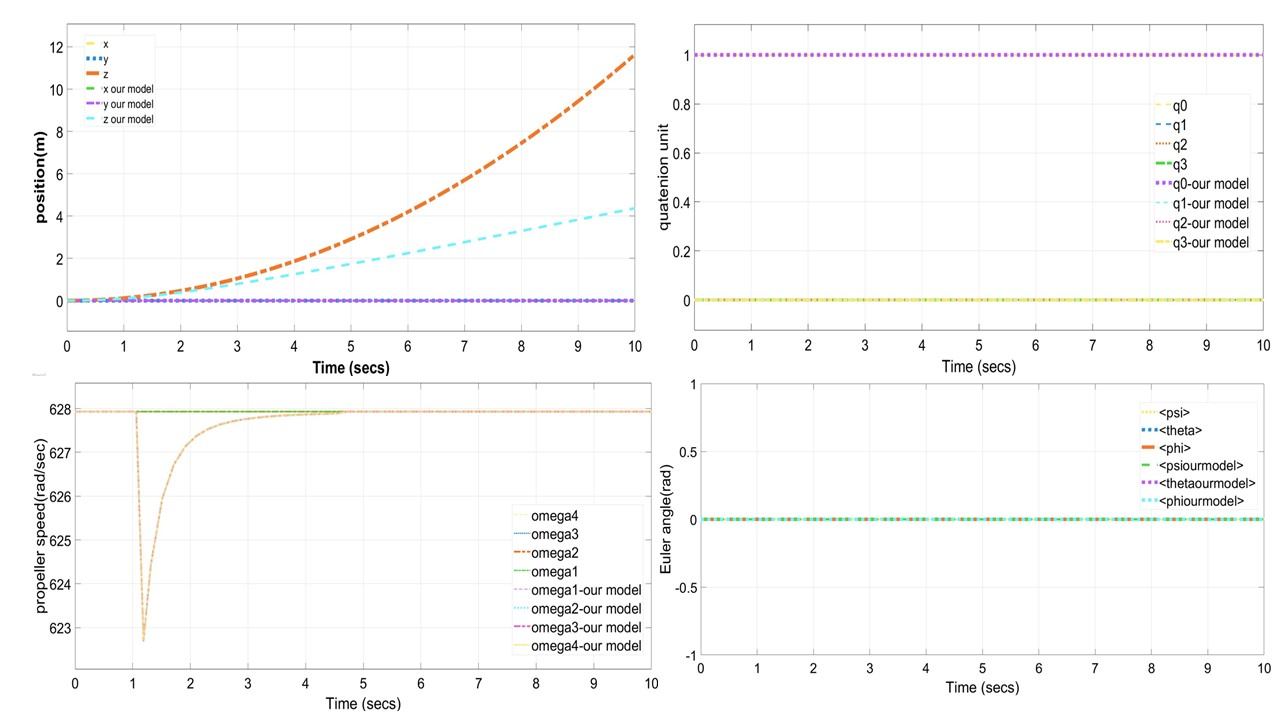
\includegraphics[width=1.0\linewidth]{figures/AscendingBest.jpg}
   % 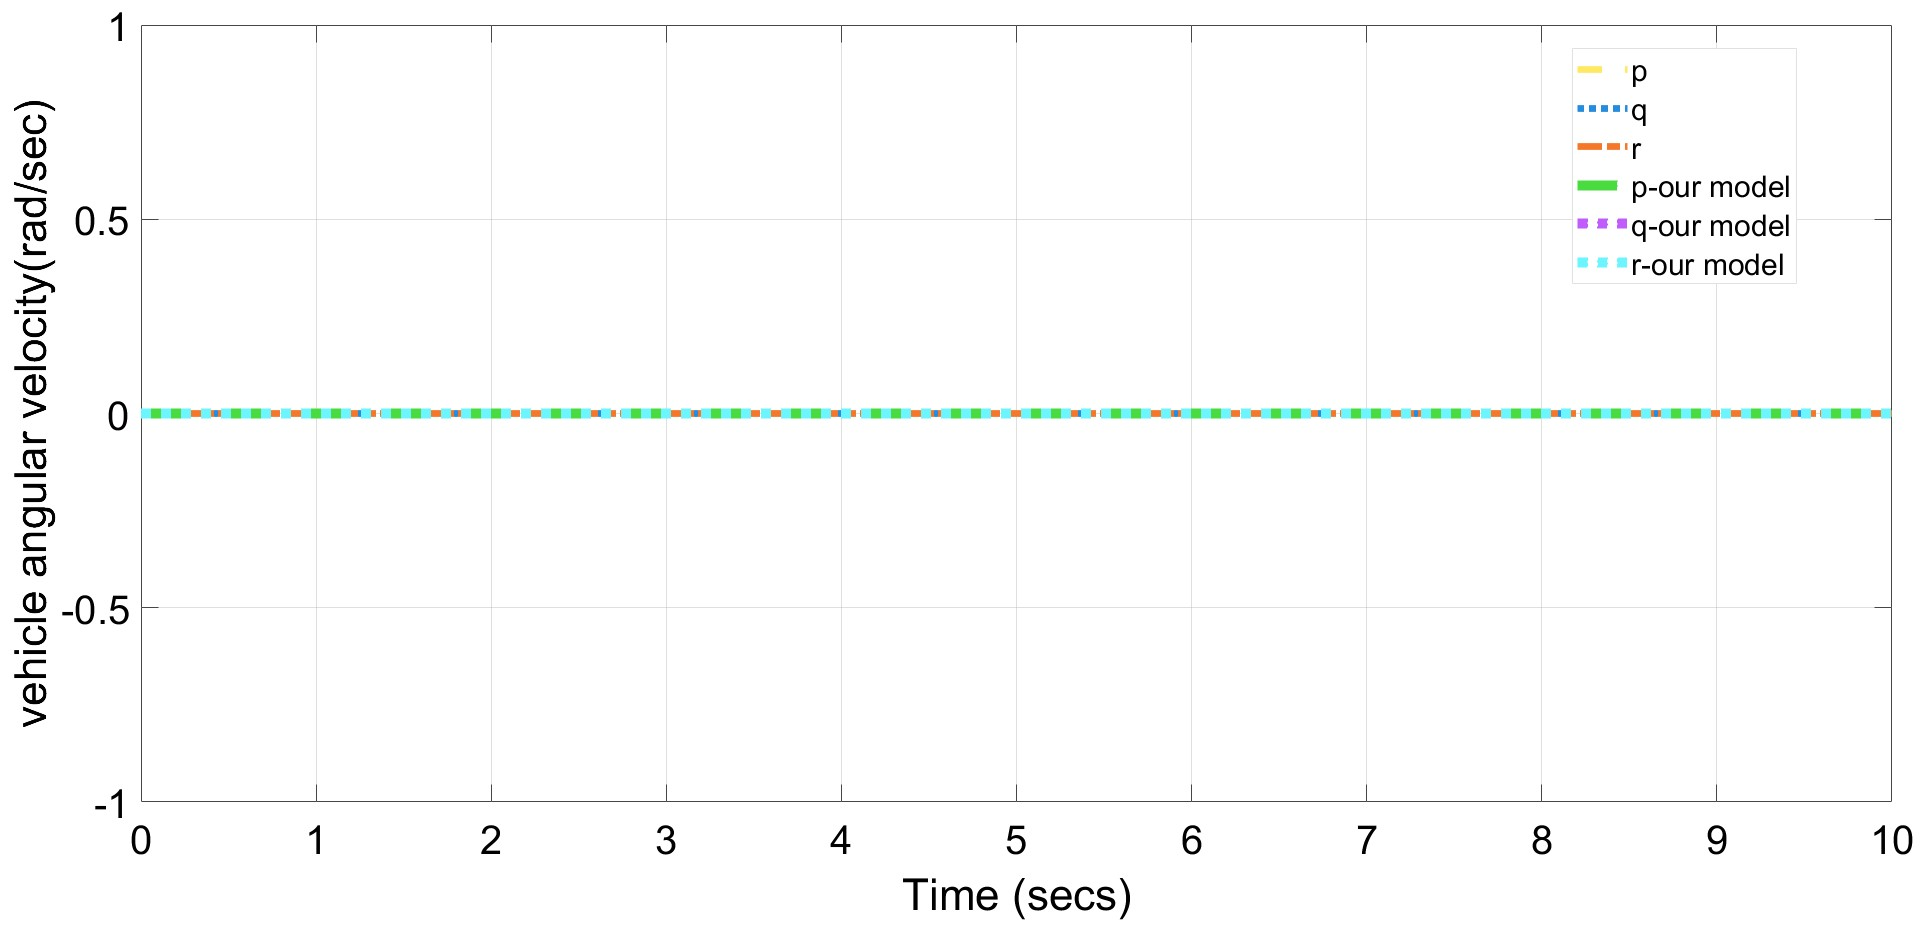
\includegraphics[width=1.0\linewidth]{figures/angularvelocityvehicle.jpg}
    %\caption{Quadrotor state for ascending maneuvering when $U_{1} > mg$}
   % \label{fig:Quad position and ground effect-ascending}
%\end{figure}

%%%%%%%%%%%%%%%%%%%%%%%%%%%%%%%%%%%%%%%%%%%
\begin{figure}[h!]
    \centering
    \begin{minipage}{0.48\linewidth}
        \centering
        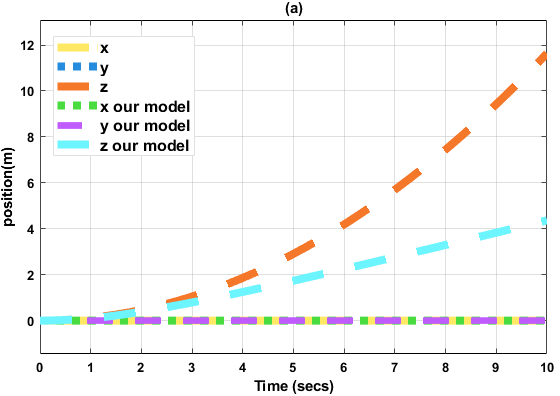
\includegraphics[width=1.0\linewidth]{figures/ascendingposition-BEST.png}
    \end{minipage}
    \hfill
    \begin{minipage}{0.48\linewidth}
        \centering
       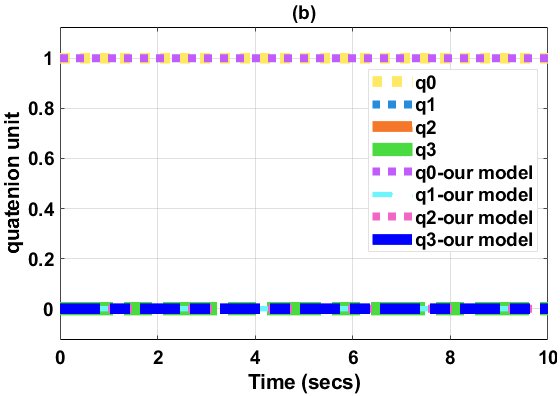
\includegraphics[width=1\linewidth]{figures/quaternion ascending-BEST.png}
    %\caption{Altitude controller diagram for maintaining desired quadrotor altitude}
    %\label{fig:attitude controller}
    \end{minipage}
\begin{minipage}{0.48\linewidth}
        \centering
        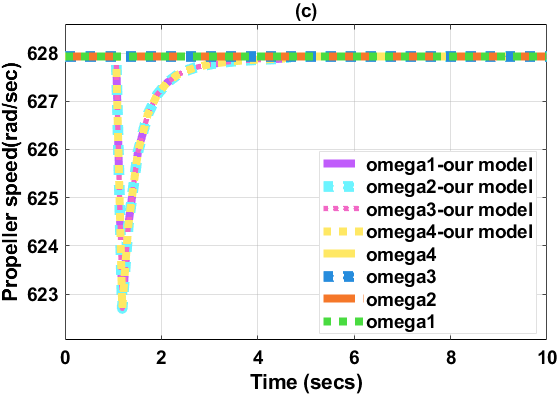
\includegraphics[width=1.0\linewidth]{figures/propeller speed-BEST.png}
    \end{minipage}
    \begin{minipage}{0.48\linewidth}
        \centering
        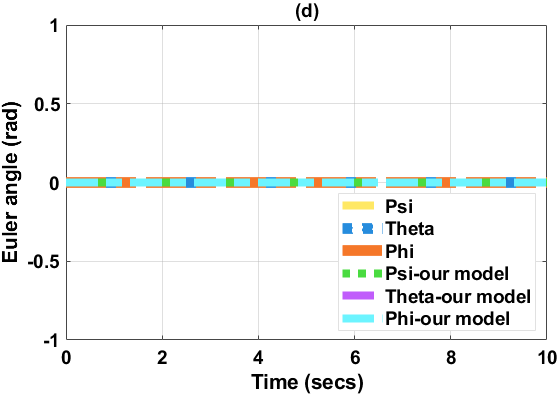
\includegraphics[width=1.0\linewidth]{figures/euler angle -BEST.png}
    \end{minipage}
    \begin{minipage}{0.48\linewidth}
        \centering
        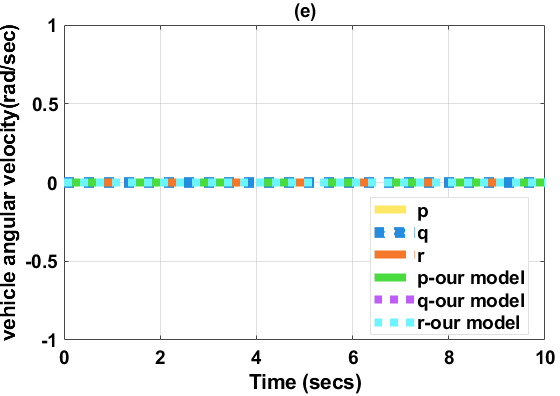
\includegraphics[width=1.0\linewidth]{figures/vehicle angular velocity-BEST.png}
    \end{minipage}
    \caption{Quadrotor state for ascending maneuvering when $U_{1} > mg$}
    \label{fig:Quad position and ground effect-ascending}
\end{figure}




%\textbf{Hovering state}: The quadrotor is first initialized at an altitude of $9\,\text{m}$. 
%Then the total thrust is set to $U_{1}=4.591\,N$, which is equal to the gravitational force. Under this condition, the quadrotor maintains a hovering state. Since no rotational motion occurs about any axis, the scalar part of the quaternion remains one while the vector components are zero, as illustrated in Figure~\ref{fig:hovering_state}.

\textbf{Hovering state}: The quadrotor is first initialized at an altitude of $9\,\text{m}$, 
then the total thrust is set to $U_{1}=4.591\,N$, which is equal to 
the gravitational force.
Figure ~\ref{fig:hovering_state} illustrates the hovering condition where thrust exactly balances the vehicle weight, resulting in a constant altitude. The position responses confirm this equilibrium, with the \(z\)-axis remaining steady at 9 m and no observable drift in the \(x\) and \(y\) directions for both models. Propeller speeds converge to identical constant values, indicating uniform thrust distribution required to sustain hover. The Euler angles remain at zero throughout, confirming the absence of roll, pitch, and yaw motion, while the quaternion representation maintains \(q_0 \approx 1\) and \(q_1, q_2, q_3 \approx 0\), consistent with a level orientation. Additionally, vehicle angular velocities are effectively zero, reflecting stable attitude dynamics. Both models exhibit similar steady-state behavior; however, the proposed model shows slightly smoother convergence, suggesting improved physical realism and damping due to aerodynamic effects, thereby enhancing confidence in its practical applicability.

%\begin{figure}[h!]
   % \centering
   % 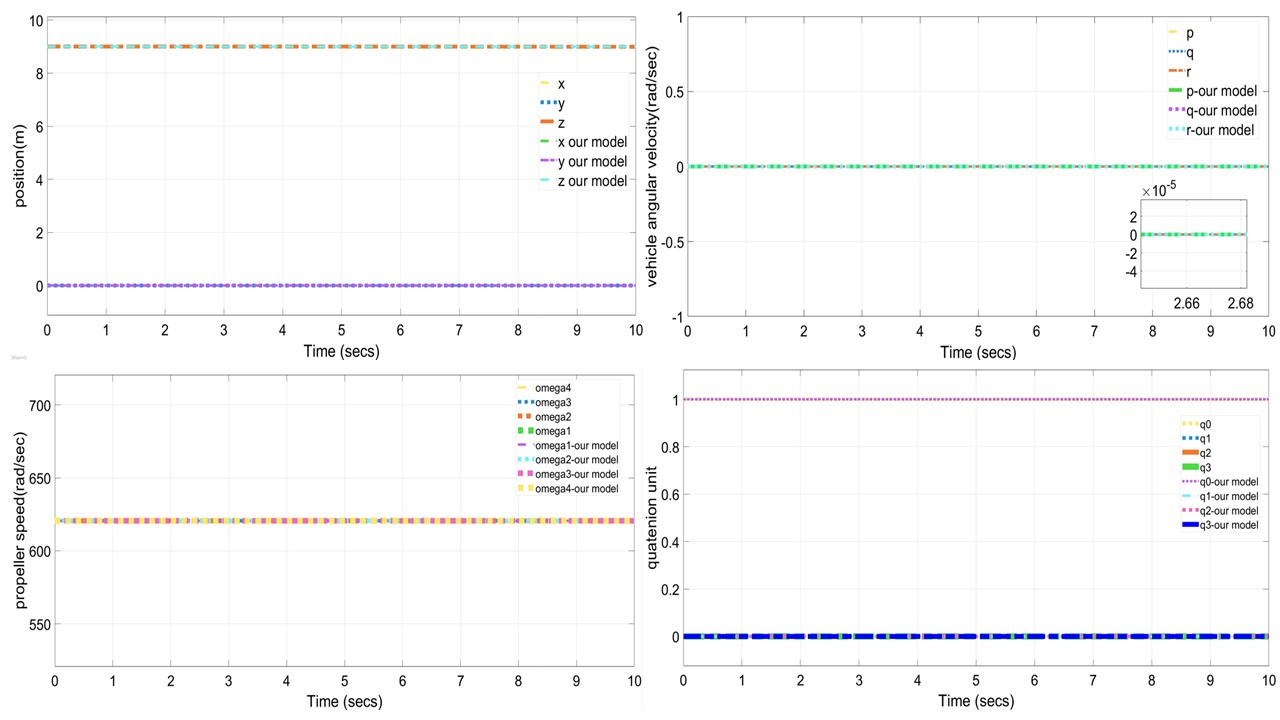
\includegraphics[width=1.0\linewidth]{figures/hoverfiguresvalidation.jpg}
    %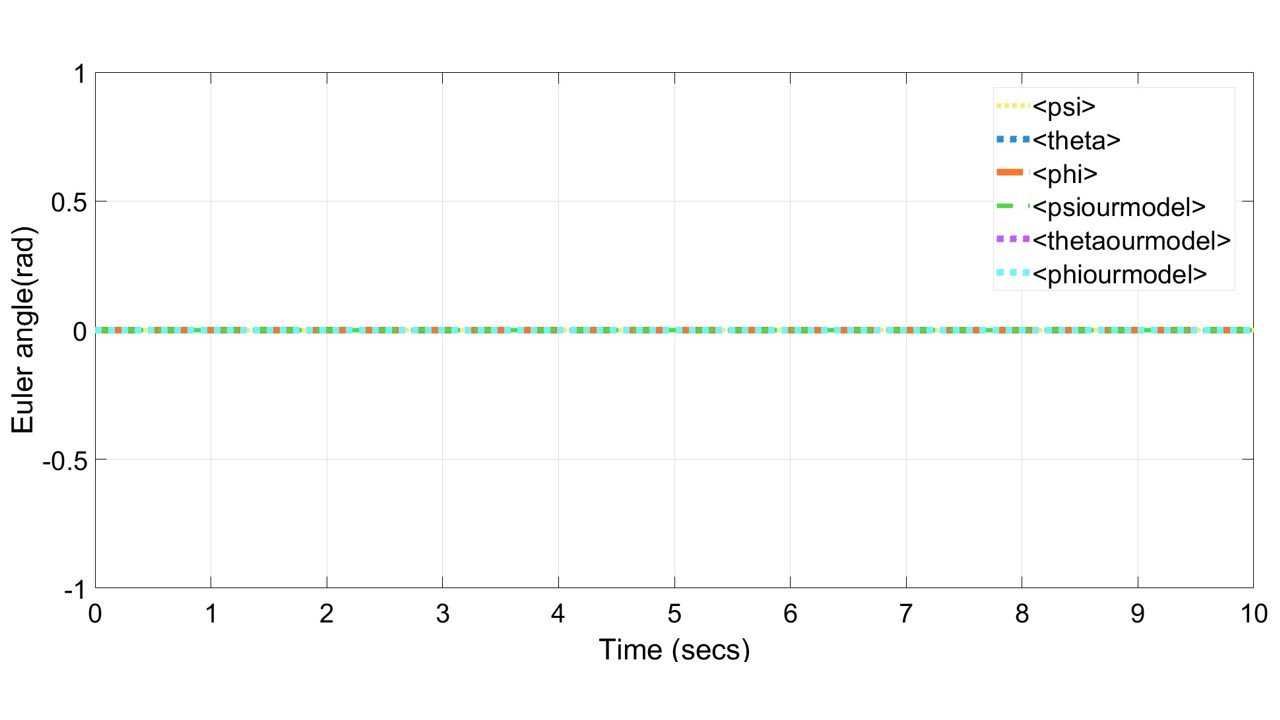
\includegraphics[width=1.0\linewidth]{figures/hovereulerangle.jpg}
   % \caption{At Hovering state when $U_{1} = mg$}
   % \label{fig:hovering_state}
%\end{figure}

\begin{figure}[h!]
    \centering
    \begin{minipage}{0.48\linewidth}
        \centering
        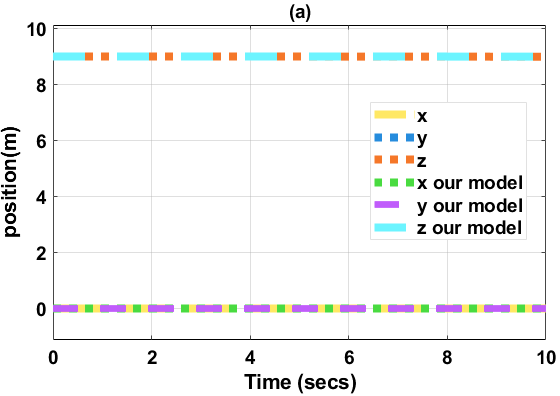
\includegraphics[width=1.0\linewidth]{figures/hover-position-BEST.png}
    \end{minipage}
    \hfill
    \begin{minipage}{0.48\linewidth}
        \centering
       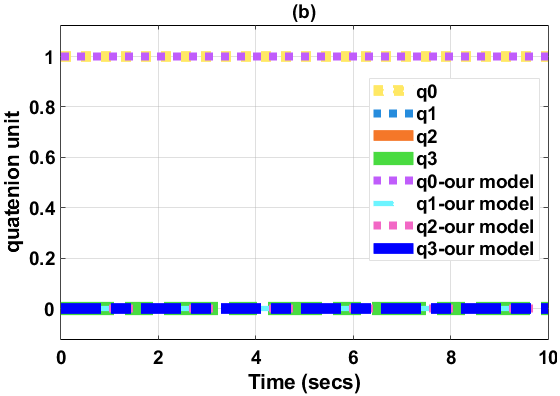
\includegraphics[width=1\linewidth]{figures/hover-quaternion-BEST.png}
    %\caption{Altitude controller diagram for maintaining desired quadrotor altitude}
    %\label{fig:attitude controller}
    \end{minipage}
\begin{minipage}{0.48\linewidth}
        \centering
        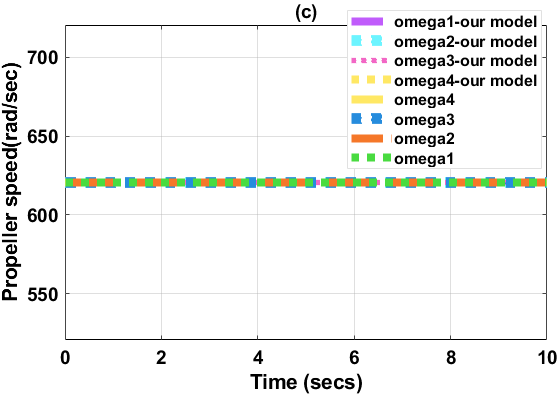
\includegraphics[width=1.0\linewidth]{figures/hover-propeller speed-BEST.png}
    \end{minipage}
    \begin{minipage}{0.48\linewidth}
        \centering
        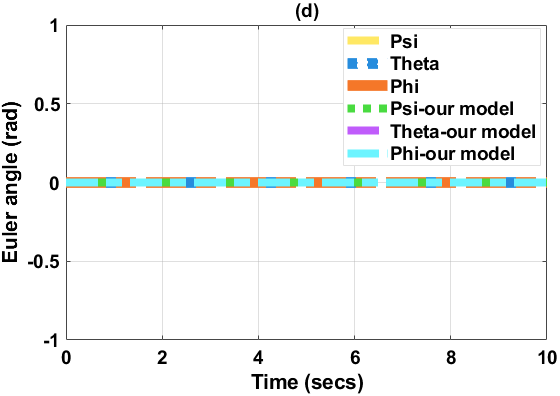
\includegraphics[width=1.0\linewidth]{figures/hover-euler-BEST.png}
    \end{minipage}
    \begin{minipage}{0.48\linewidth}
        \centering
        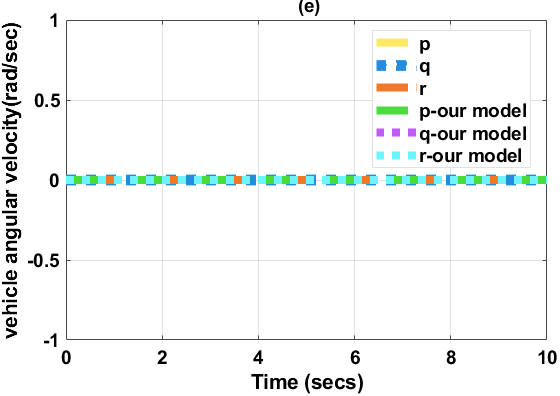
\includegraphics[width=1.0\linewidth]{figures/hover-vehicle velocity-BEST.png}
    \end{minipage}
    \caption{At Hovering state when $U_{1} = mg$}
   \label{fig:hovering_state}
\end{figure}



%\textbf{Roll rotation} :At the hovering state, the roll control torque is set to $U_{2}=0.2\,Nm$ while 
%keeping $U_{1}$ constant. This increases the speeds of motors 1 and 4 and 
%decreases those of motors 2 and 3, producing roll motion toward the positive 
%$y$-direction. Since the open-loop system is unstable, the quadrotor continues 
%to rotate about the $x$-axis. When the roll angle $\phi \geq \tfrac{\pi}{2}$, 
%the vehicle loses lift and falls rapidly to the ground, as illustrated in 
%Figure~\ref{fig:roll_rotation}.

\textbf{Roll rotation} :At the hovering state, the roll control torque is set to $U_{2}=0.2\,Nm$ while 
keeping $U_{1}$ constant, Figure ~\ref {fig:roll_rotation} confirms the expected open-loop roll instability of the quadrotor when a constant roll torque is applied during hover. The position responses show rapid altitude loss and growing lateral displacement, indicating that once the vehicle tilts significantly, part of the thrust is redirected from vertical support to rotational and lateral motion. This effect is more pronounced in the baseline model, whereas the proposed model exhibits a slightly moderated response due to the inclusion of aerodynamic and drag effects. The propeller speeds split into two groups, consistent with the roll command generation mechanism. The Euler angles reveal continuous growth of roll, while pitch and yaw remain comparatively small. The quaternion trajectories depart from their hover values, confirming progressive attitude deviation from level flight. Likewise, the angular velocity about the roll axis increases steadily, while the other rates remain close to zero. Thus the enhanced model gives a more physically realistic description of roll-induced loss of stability.

%\begin{figure}[h!]
   % \centering
   % 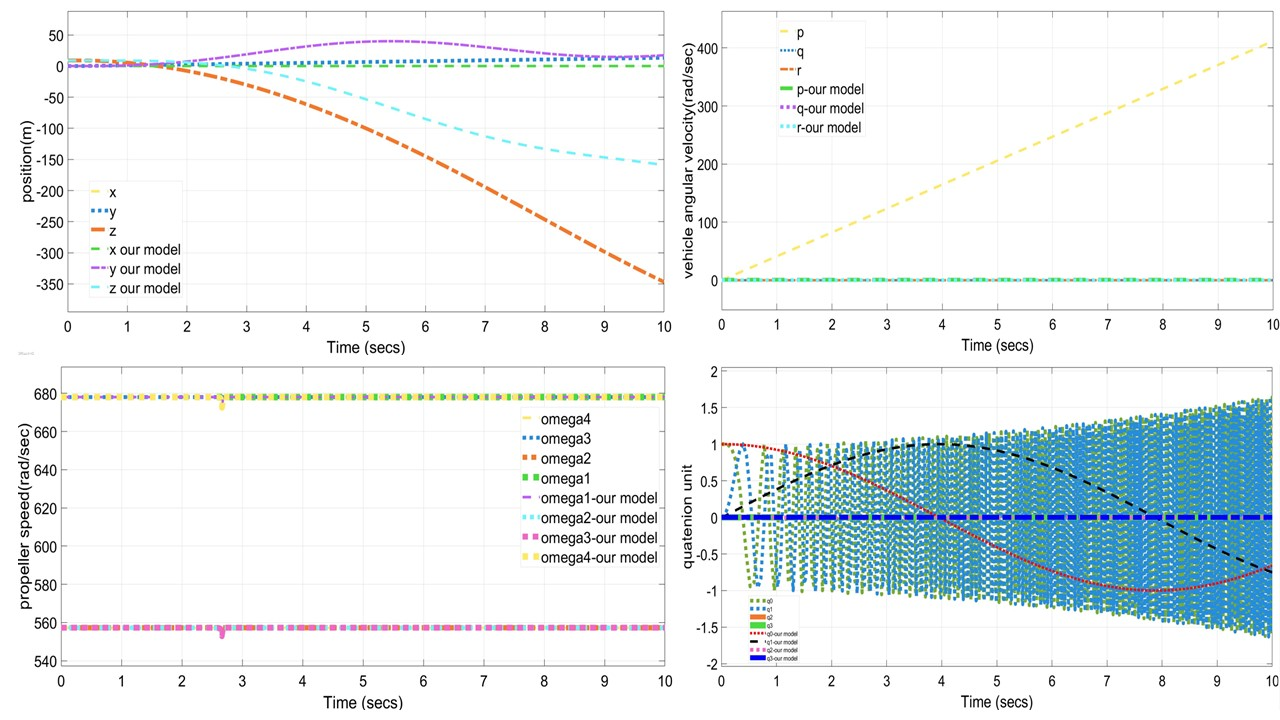
\includegraphics[width=1.0\linewidth]{figures/rollBest.jpg}
   % 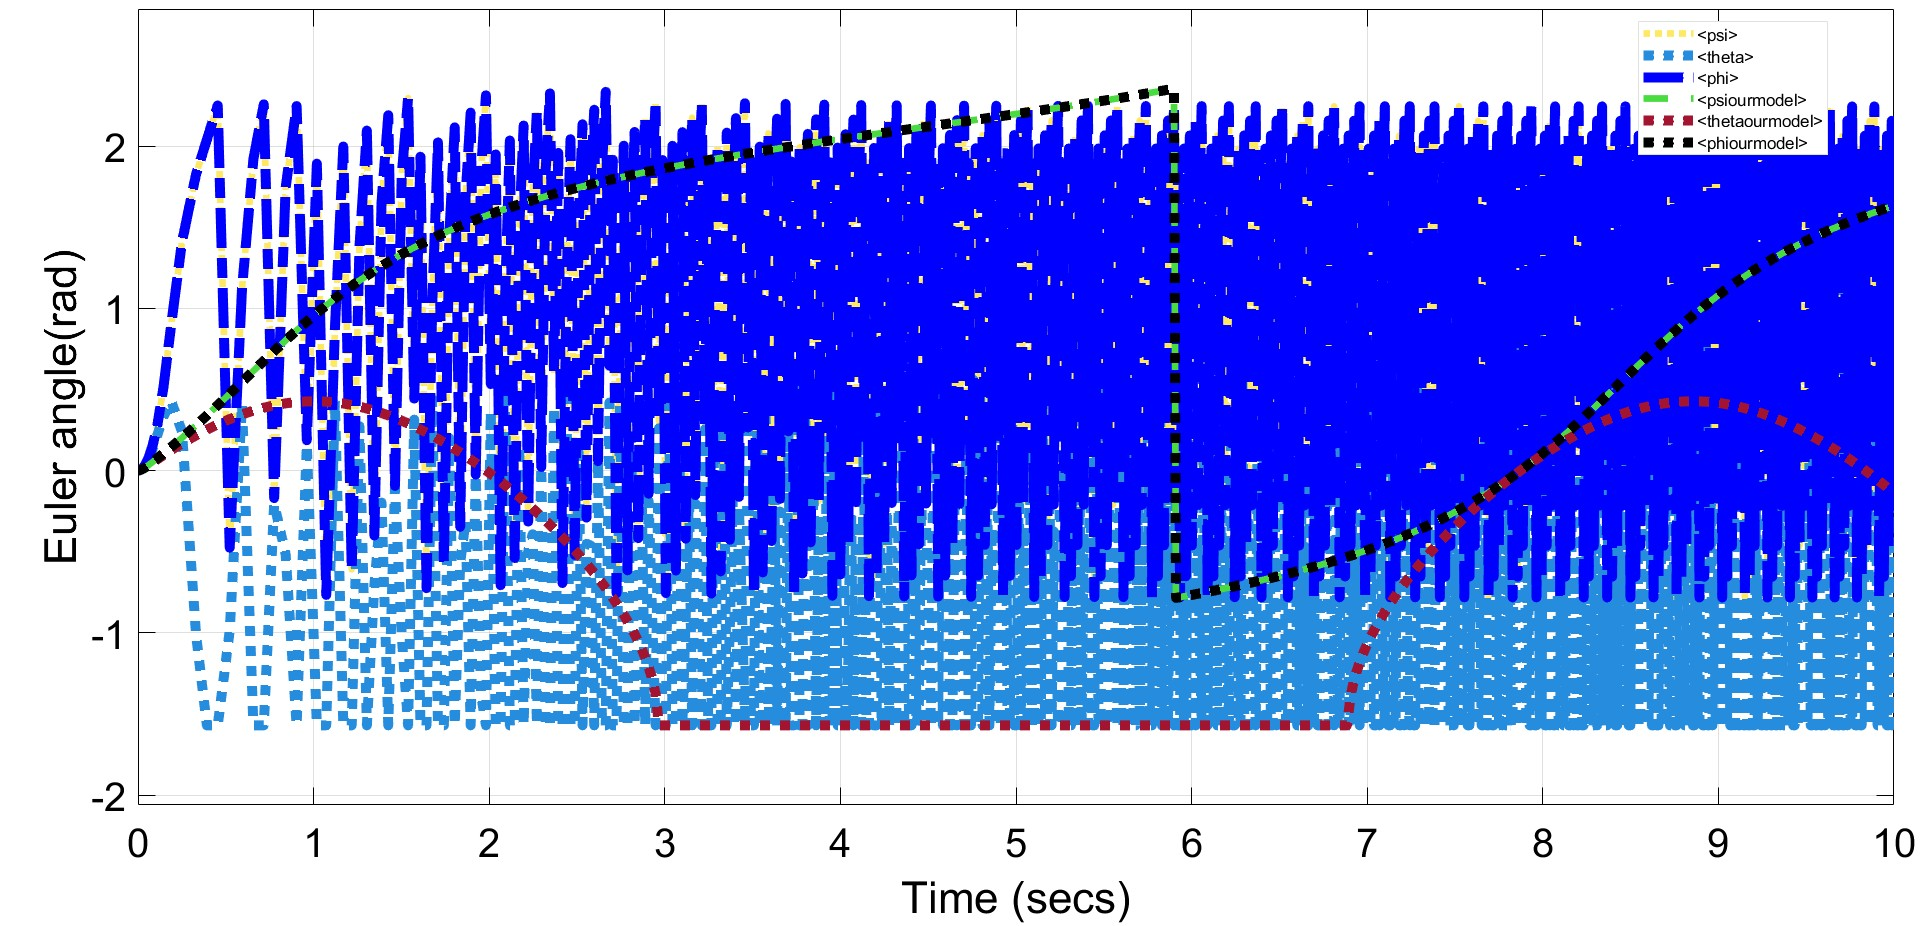
\includegraphics[width=1.0\linewidth]{figures/rolleuler.jpg}
   % \caption{Roll rotation due to $U_{1} = mg$ and $U_{2} = 0.2\,Nm$}
   % \label{fig:roll_rotation}
%\end{figure}

\begin{figure}[h!]
    \centering
    \begin{minipage}{0.48\linewidth}
        \centering
        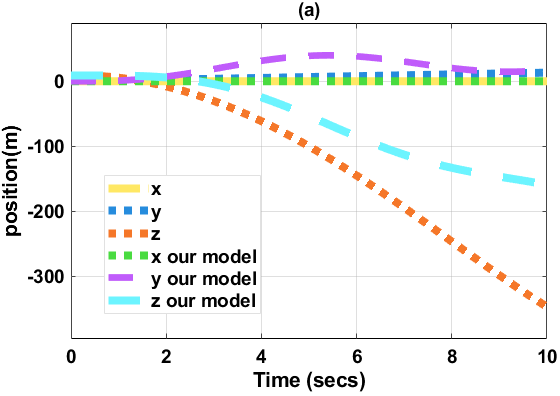
\includegraphics[width=1.0\linewidth]{figures/roll-position-BEST.png}
    \end{minipage}
    \hfill
    \begin{minipage}{0.48\linewidth}
        \centering
       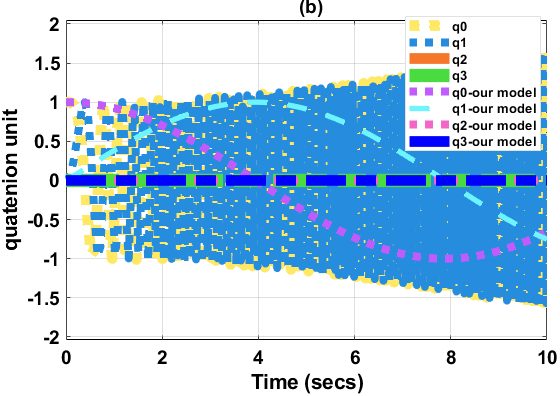
\includegraphics[width=1\linewidth]{figures/roll-quaternion-BEST.png}
    %\caption{Altitude controller diagram for maintaining desired quadrotor altitude}
    %\label{fig:attitude controller}
    \end{minipage}
\begin{minipage}{0.48\linewidth}
        \centering
        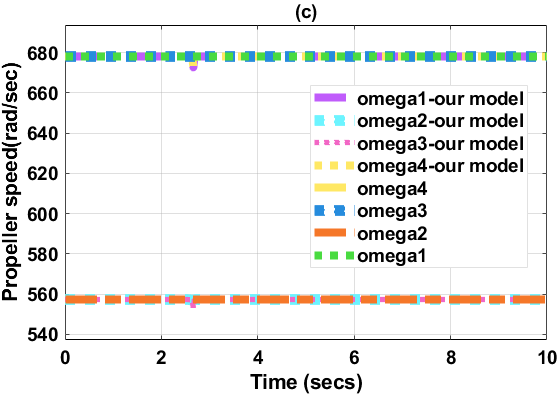
\includegraphics[width=1.0\linewidth]{figures/roll-propeller speed-BEST.png}
    \end{minipage}
    \begin{minipage}{0.48\linewidth}
        \centering
        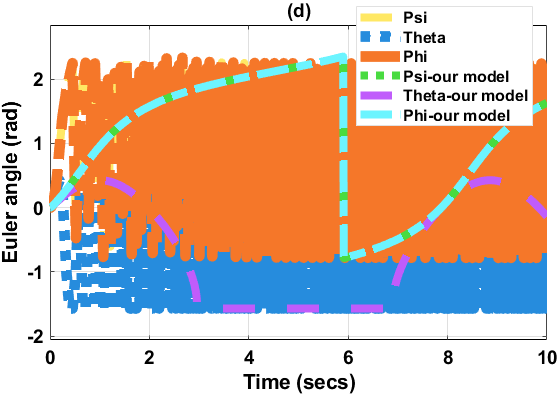
\includegraphics[width=1.0\linewidth]{figures/roll-euler-BEST.png}
    \end{minipage}
    \begin{minipage}{0.48\linewidth}
        \centering
        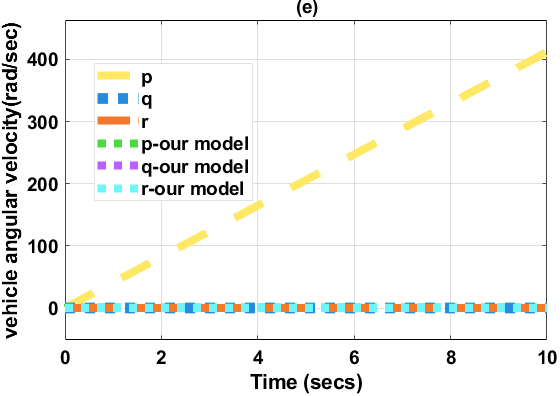
\includegraphics[width=1.0\linewidth]{figures/roll-vehicle speed-BEST.png}
    \end{minipage}
    \caption{Roll rotation due to $U_{1} = mg$ and $U_{2} = 0.2\,Nm$}
    \label{fig:roll_rotation}
\end{figure}


%\textbf{Pitch rotation} : At hovering, the pitch control torque is set to $U_{3}=0.2\,Nm$ while keeping $U_{1}$ constant. 
%This increases the speeds of motors 1 and 2 and decreases those of motors 3 and 4, 
%causing motion along the negative $x$-direction. Similar to roll, when the pitch angle 
%$\theta \geq \tfrac{\pi}{2}$, the quadrotor descends rapidly due to the combined effect 
%of thrust and gravity, as shown in Figure~\ref{fig:pitch_rotation}. 

%Using the canonical Euler triple, only pitch angles in the range $[-\tfrac{\pi}{2}, \tfrac{\pi}{2}]$ 
%are shown in the Euler-angle rotation graph. In contrast, the quaternion representation 
%allows rotation beyond this range without instability, demonstrating its singularity-free property.

\textbf{Pitch rotation} : At hovering, the pitch control torque is set to $U_{3}=0.2\,Nm$ while keeping $U_{1}$ constant.
Figure ~\ref{fig:pitch_rotation} illustrates the open-loop pitch response when a constant pitch torque is applied at hover. The position plots show a pronounced displacement in the longitudinal direction together with a rapid loss of altitude, confirming that once the vehicle pitches significantly, the thrust vector is no longer aligned with the vertical axis and can no longer fully balance weight. This effect develops faster in the baseline model, while the proposed model shows a slightly moderated fall due to aerodynamic drag. The propeller speeds separate into two steady groups, consistent with the control action required to generate pitching motion. The Euler-angle response indicates continuous growth of pitch, whereas roll and yaw remain close to zero. As expected, the quaternion states evolve smoothly beyond the Euler-angle range, confirming their suitability for representing large rotations without singularity. Similarly, the pitch-rate response increases steadily, while the other angular velocities remain small. Thus, the enhanced model captures pitch-induced instability more realistically.




%\begin{figure}[h!]
   % \centering
    %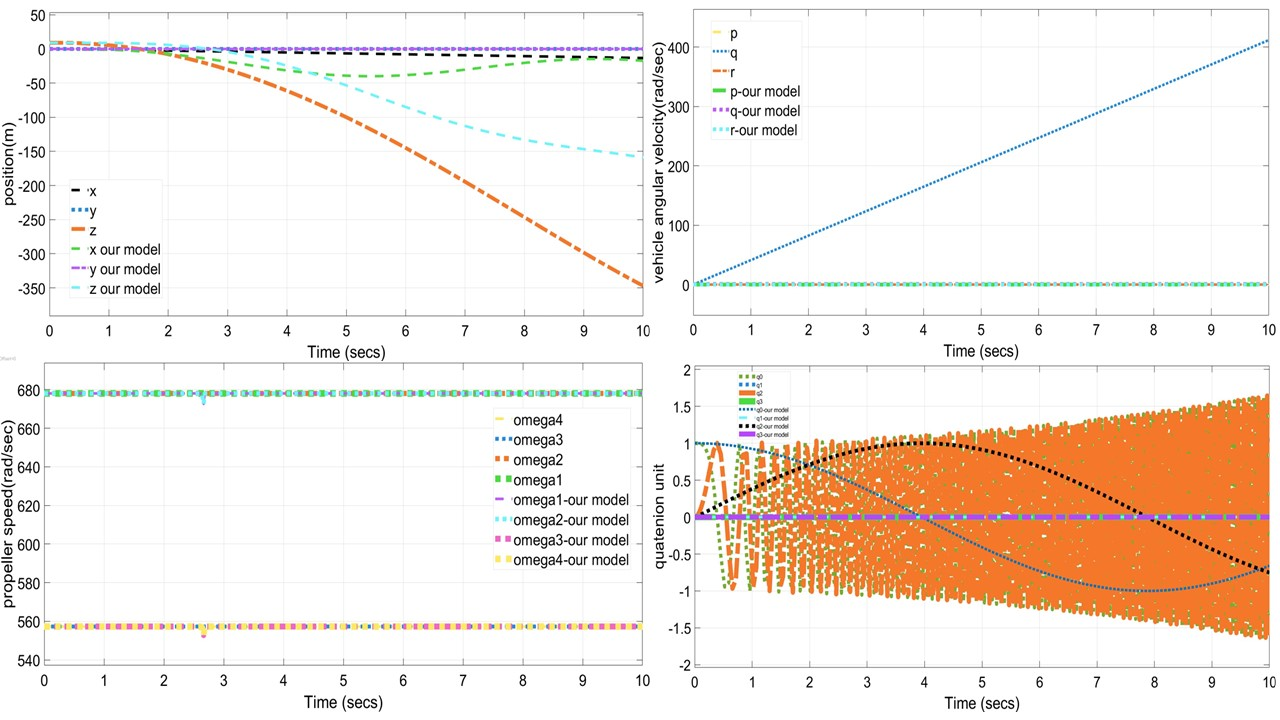
\includegraphics[width=1.0\linewidth]{figures/pitchBest.jpg}
   % 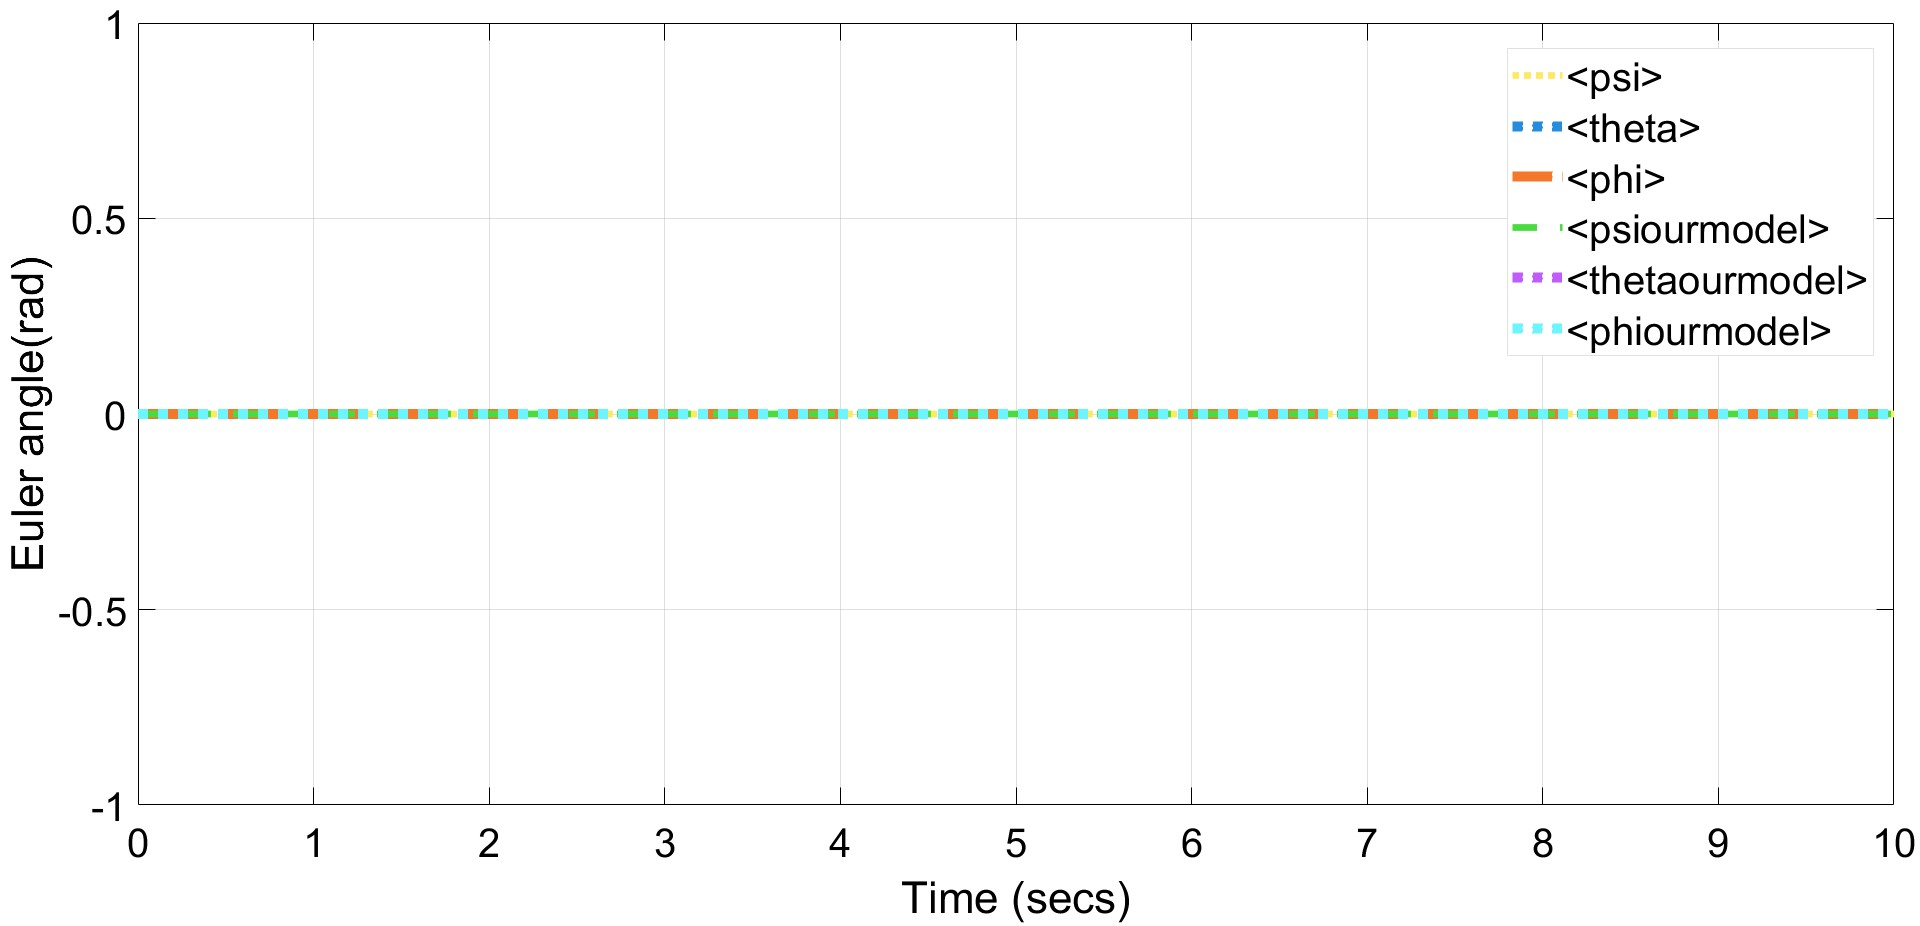
\includegraphics[width=1.0\linewidth]{figures/euleranglepitch.jpg}
    %\caption{Pitch rotation due to $U_{1} = mg$ and $U_{3} = 0.2\,Nm$}
    %\label{fig:pitch_rotation}
%\end{figure}

\begin{figure}[h!]
    \centering
    \begin{minipage}{0.48\linewidth}
        \centering
        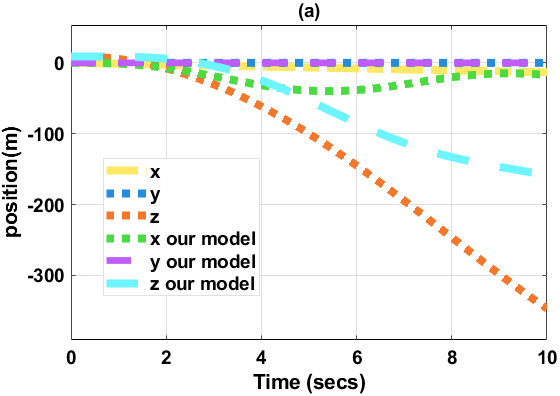
\includegraphics[width=1.0\linewidth]{figures/pitch-position-BEST.png}
    \end{minipage}
    \hfill
    \begin{minipage}{0.48\linewidth}
        \centering
       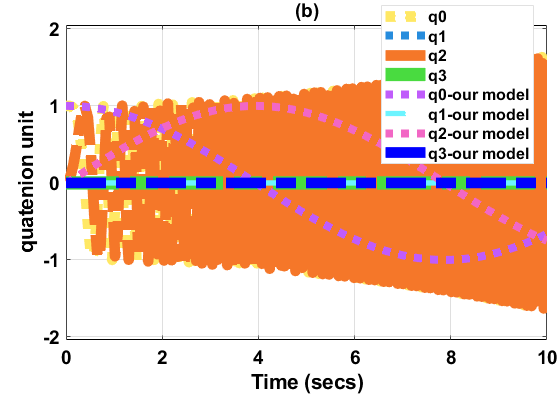
\includegraphics[width=1\linewidth]{figures/pitch-quaternion-BEST.png}
    %\caption{Altitude controller diagram for maintaining desired quadrotor altitude}
    %\label{fig:attitude controller}
    \end{minipage}
\begin{minipage}{0.48\linewidth}
        \centering
        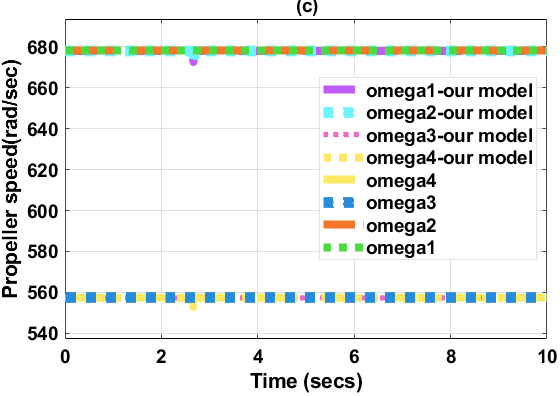
\includegraphics[width=1.0\linewidth]{figures/pitch-propeller speed-BEST.png}
    \end{minipage}
    \begin{minipage}{0.48\linewidth}
        \centering
        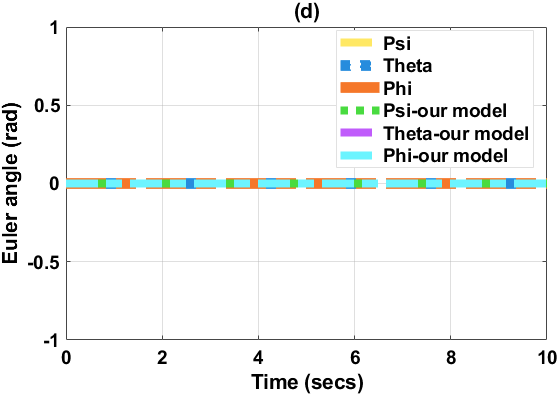
\includegraphics[width=1.0\linewidth]{figures/pitch-euler-BEST.png}
    \end{minipage}
    \begin{minipage}{0.48\linewidth}
        \centering
        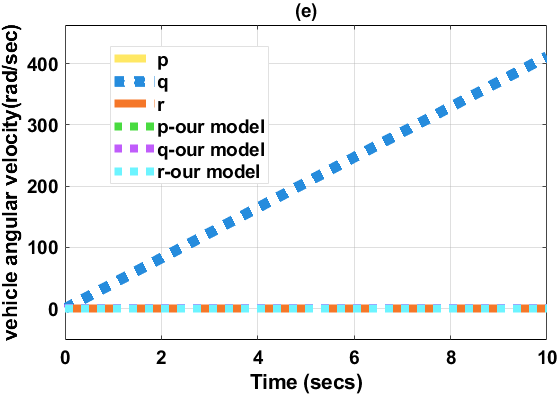
\includegraphics[width=1.0\linewidth]{figures/pitch-vehicle speed-BEST.png}
    \end{minipage}
    \caption{Pitch rotation due to $U_{1} = mg$ and $U_{3} = 0.2\,Nm$}
    \label{fig:pitch_rotation}
\end{figure}



%\textbf{The last scenario for Yaw rotation:} 
%At hovering, the yaw control torque is set to $U_{4} = 0.2\,Nm$, causing the quadrotor to rotate clockwise about the $z$-axis. This increases the speeds of motors 2 and 4 and decreases those of motors 1 and 3, while keeping $U_{1}$ (altitude) constant. No lateral motion along $x$ or $y$ occurs. By increasing the speed of propellers rotating in the same direction and decreasing the opposite ones, a net angular velocity is generated, resulting in a nonzero residual propeller speed $\Omega_r \neq 0$, as shown in Figure~\ref{fig:yaw_rotation}.

\textbf{The last scenario for Yaw rotation:} 
At hovering, the yaw control torque is set to $U_{4} = 0.2\,Nm$, causing the quadrotor 
to rotate clockwise about the $z$-axis. Figure ~\ref{fig:yaw_rotation} presents the yaw-rotation validation under a constant yaw torque while the total thrust is maintained at the hover condition. The position responses remain nearly constant, with altitude preserved around 9 m and no noticeable motion along the \(x\)- or \(y\)-axes, confirming that the applied input primarily excites rotational motion about the vertical axis. The propeller-speed plots show the expected split between counter-rotating motor pairs, which generates the required reaction torque for clockwise yaw. The Euler-angle response indicates that yaw evolves while roll and pitch remain essentially zero, confirming decoupled rotational behavior in this maneuver. The quaternion components vary consistently with pure heading rotation and remain bounded, showing smooth attitude representation throughout the motion. Similarly, the angular velocity response is dominated by the yaw rate, while roll and pitch rates stay close to zero. Overall, both models reproduce the expected yaw behavior, although the enhanced model remains more physically representative.


%\begin{itemize}
   % \item During roll and pitch maneuvers, propellers generate positive $U_2$ and $U_3$ 
   % for half the cycle and negative for the other half, producing back-and-forth 
   % lateral motion, as seen in Figures~\ref{fig:roll_rotation} and \ref{fig:pitch_rotation}.
    
   % \item Using the canonical Euler triple, roll and yaw angles in 
   % Figures~\ref{fig:roll_rotation} and \ref{fig:yaw_rotation} remain within 
   % $[-\pi, \pi]$.
%\end{itemize}

%The simulation results confirm that the derived quadrotor dynamic model behaves 
%as expected, validating its feasibility.
%Following this quantitative analysis, the next subsection focuses on the qualitative stability analysis at the operating point.

 %\begin{figure}[h!]
    % \centering
    %\includegraphics[width=0.6\textwidth]{your-yaw-figure.png} % insert figure here
    % 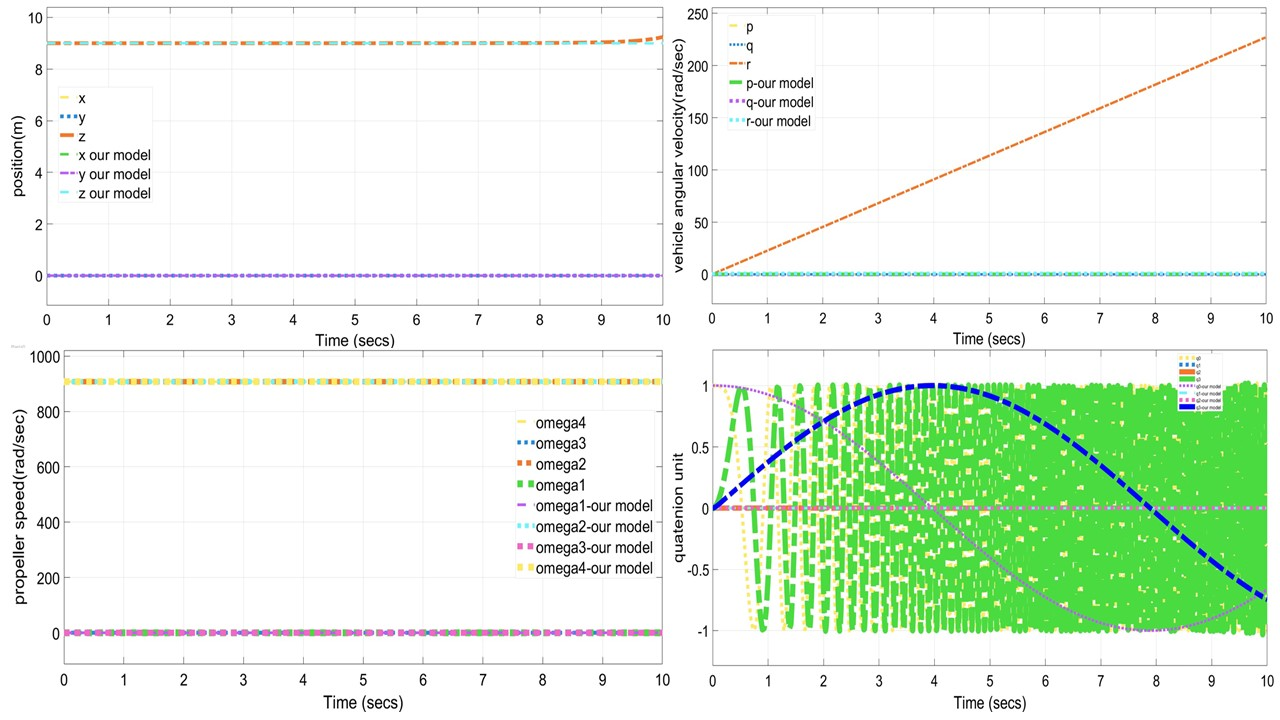
\includegraphics[width=1.0\linewidth]{figures/yawBest.jpg}
     %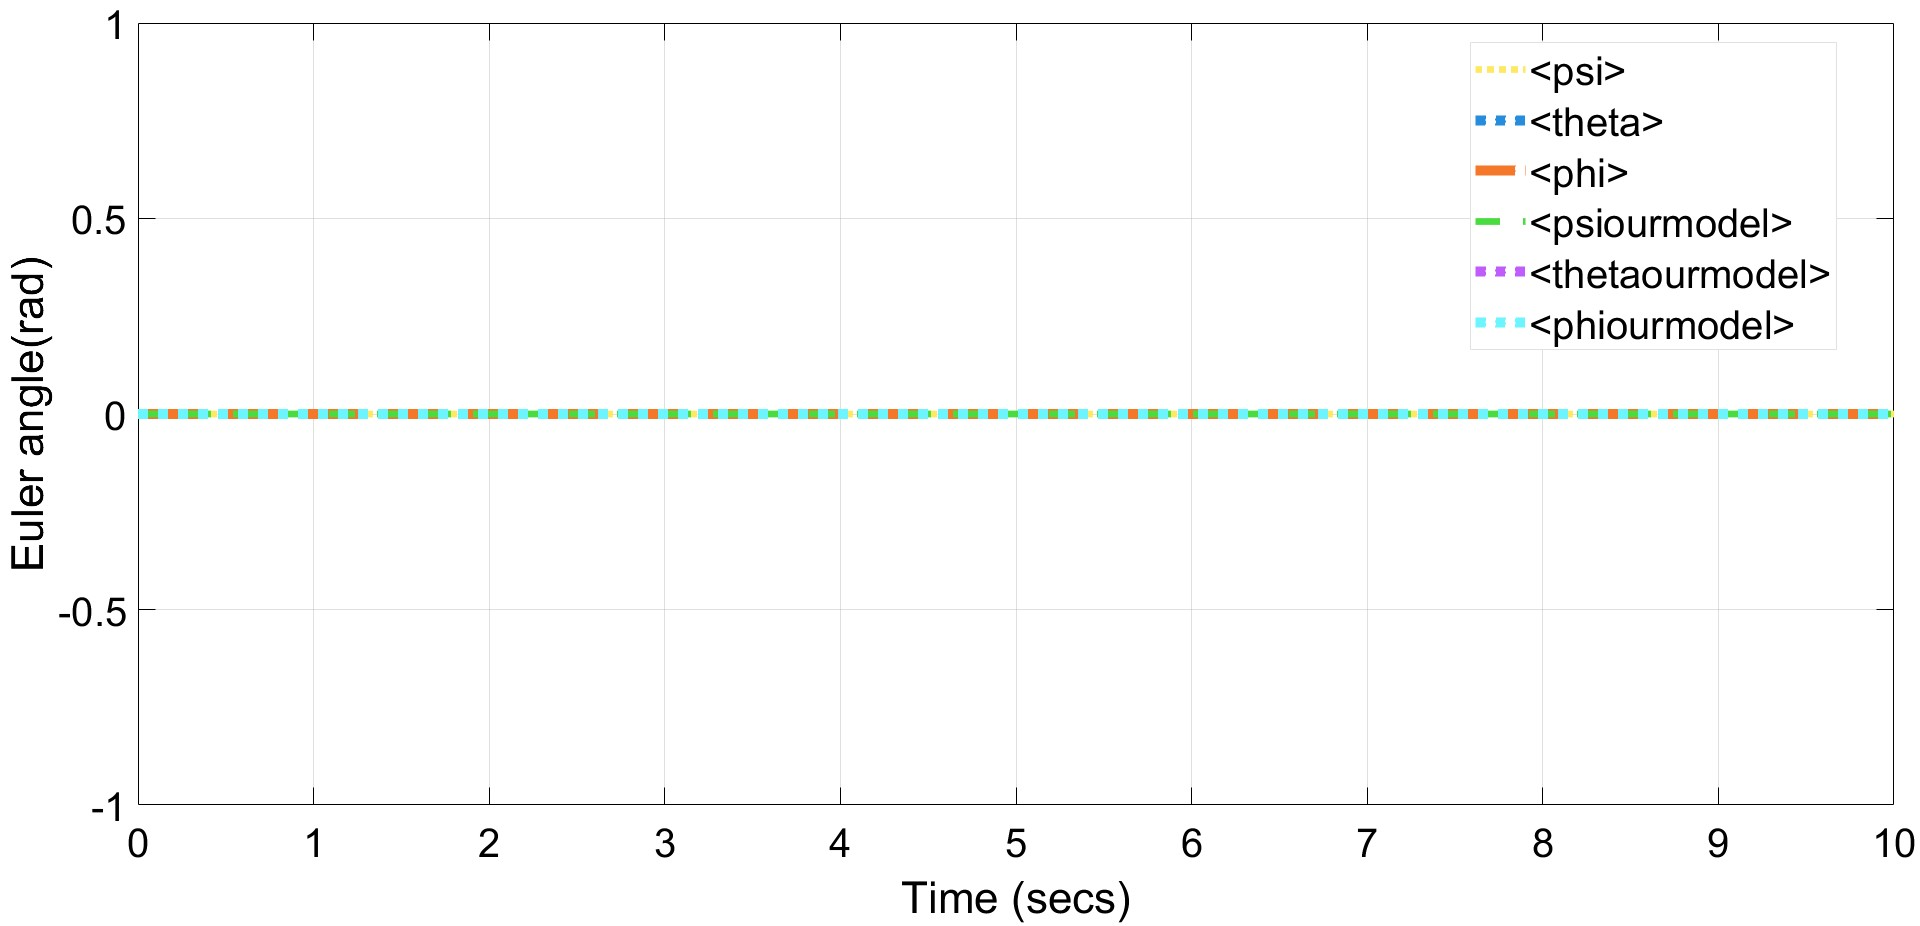
\includegraphics[width=1.0\linewidth]{figures/euleryaw.jpg}
     %\caption{CW yaw rotation due to $U_{1} = mg$ and $U_{4} = 0.2\,Nm$}
     %\label{fig:yaw_rotation}
 %\end{figure}

\begin{figure}[h!]
    \centering
    \begin{minipage}{0.48\linewidth}
        \centering
        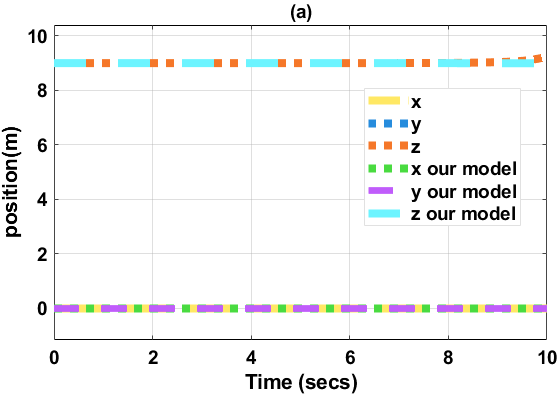
\includegraphics[width=1.0\linewidth]{figures/yaw-position-BEST.png}
    \end{minipage}
    \hfill
    \begin{minipage}{0.48\linewidth}
        \centering
       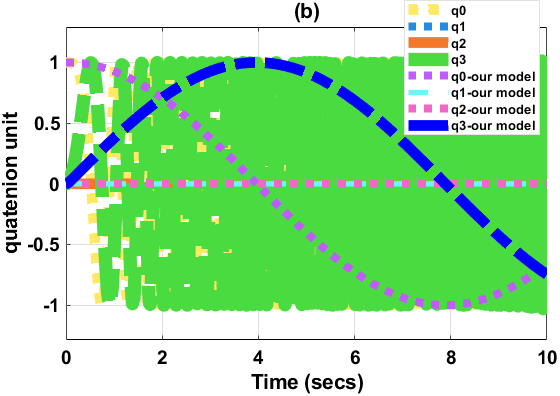
\includegraphics[width=1\linewidth]{figures/yaw-quaternion-BEST.png}
    %\caption{Altitude controller diagram for maintaining desired quadrotor altitude}
    %\label{fig:attitude controller}
    \end{minipage}
\begin{minipage}{0.48\linewidth}
        \centering
        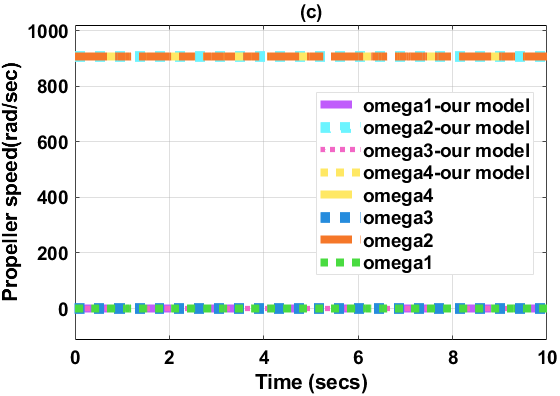
\includegraphics[width=1.0\linewidth]{figures/yaw-propeller speed-BEST.png}
    \end{minipage}
    \begin{minipage}{0.48\linewidth}
        \centering
        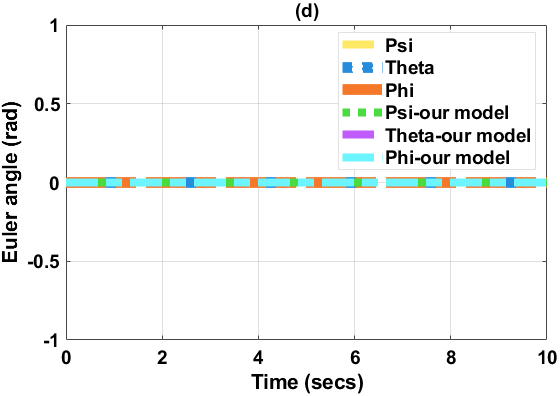
\includegraphics[width=1.0\linewidth]{figures/yaw-euler-BEST.png}
    \end{minipage}
    \begin{minipage}{0.48\linewidth}
        \centering
        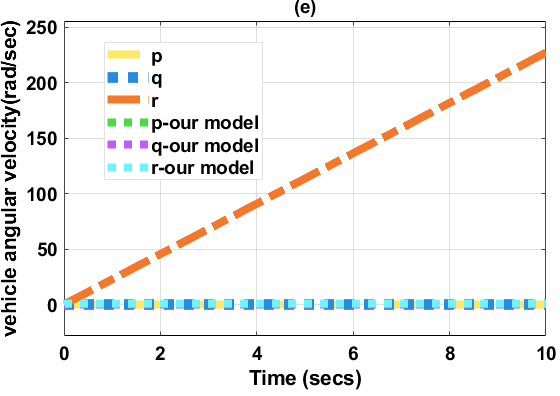
\includegraphics[width=1.0\linewidth]{figures/yaw-vehicle speed-BEST.png}
    \end{minipage}
    \caption{CW yaw rotation due to $U_{1} = mg$ and $U_{4} = 0.2\,Nm$}
    \label{fig:yaw_rotation}
\end{figure}


\begin{table}[htbp]
\centering
\caption{PSO Performance for Different Numbers of Particles in Attitude Gains Tuning}
\label{tab:PSO_ITAE_attitude}

\resizebox{\linewidth}{!}{%
\begin{tabular}{|c|c|c|c|c|}
\hline
\textbf{Nop} & \textbf{max. iteration} & \textbf{Time (minutes)} &
\textbf{1st iteration GBEST} & \textbf{100th iteration GBEST (\% improvement)} \\ \hline
15 & 100 & 30  & 10.0610 & 7.1602 (28.83\%) \\ \hline
30 & 100 & 86  & 9.0872  & 7.6509 (15.81\%) \\ \hline
45 & 100 & 105 & 8.9855  & 7.5439 (16.04\%) \\ \hline
60 & 100 & 136 & 8.4118  & 7.2328 (14.02\%) \\ \hline
75 & 100 & 167 & 9.2651  & 7.6608 (17.31\%) \\ \hline
\end{tabular}
}%
\end{table}


\begin{table}[htbp]
\centering

\caption{PSO Performance for Different Numbers of Particles in Position Gains Tuning}
\label{tab:PSO_Position_Gains}

\resizebox{\linewidth}{!}{%
\begin{tabular}{|c|c|c|c|c|}
\hline
\textbf{Nop} & \textbf{Max. Iteration} & \textbf{Time (minutes)} &
\textbf{1st iteration GBEST} & \textbf{100th iteration GBEST (\% improvement)} \\ \hline

15 & 100 & 38  & 64.1658 & 63.1375 (1.60\%) \\ \hline
30 & 100 & 60  & 70.6404 & 63.1375 (10.63\%) \\ \hline
45 & 100 & 67  & 63.6148 & 63.1375 (0.75\%) \\ \hline
60 & 100 & 93  & 63.5962 & 63.1375 (0.72\%) \\ \hline
75 & 100 & 105 & 63.5222 & 63.1375 (0.61\%) \\ \hline

\end{tabular}
}
\end{table}

\section{PSO tunning results}
%Below figure shows how ITAE values were changing with respect to number of particle swarm size  during attitude and position controller gains optimization see Fig.\ref{fig:Attitude ITAE} and Fig.\ref{fig:Position ITAE}%

The results in Tables \ref{tab:PSO_ITAE_attitude} and \ref{tab:PSO_Position_Gains}, together with  Fig.\ref{fig:Attitude ITAE} and Fig.\ref{fig:Position ITAE}, demonstrate the effectiveness of PSO in tuning the ASTSMC gains. For attitude control, a clear reduction in ITAE is observed across all particle sizes, with faster convergence achieved at lower swarm sizes, particularly Number of Particles (Nop) = 15, indicating computational efficiency without compromising performance. In contrast, position control shows minimal variation in final ITAE values, as all configurations converge to a similar optimum, suggesting a well-defined solution space. Increasing particle size mainly affects convergence behavior rather than final performance. Thus, PSO provides consistent and reliable tuning for both attitude and position dynamics.

\begin{figure}[h!]
    \centering
    \begin{minipage}{0.48\linewidth}
        \centering
        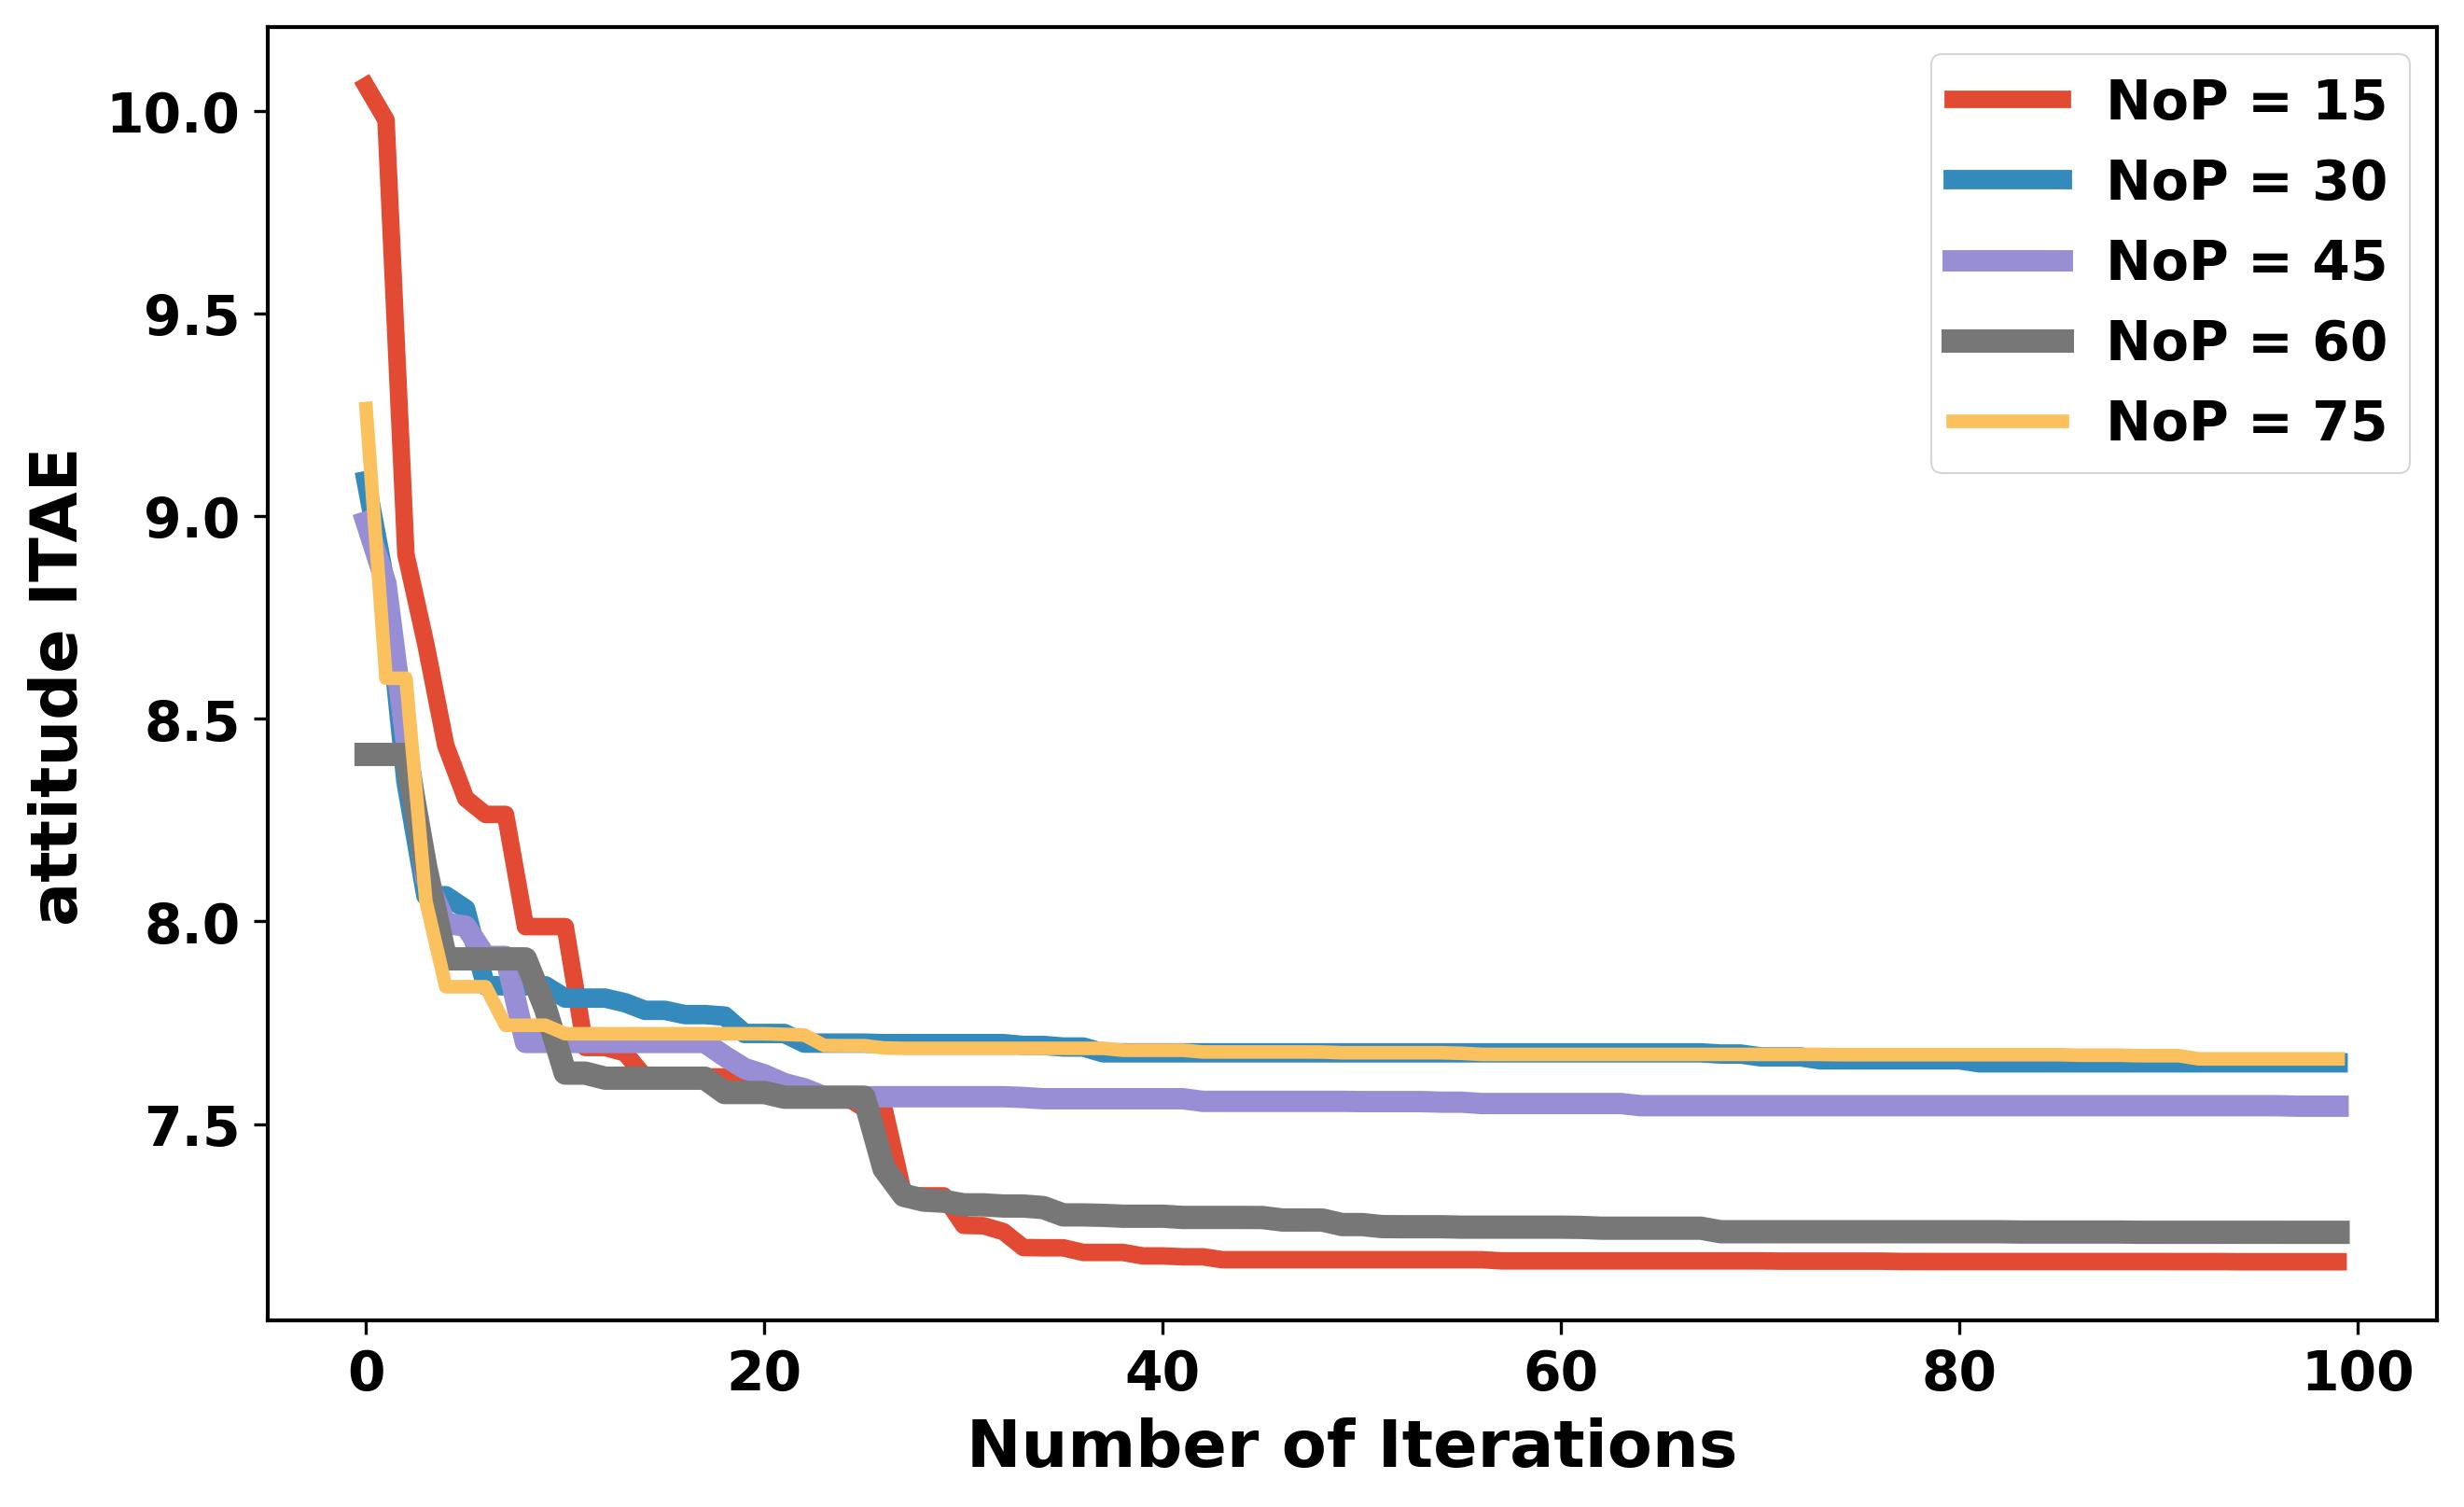
\includegraphics[width=\linewidth]{figures/attitude ITAE_plot.jpg}
        \caption{Attitude ITAE against Number of Iterations for different Particle Swarm Size}
        \label{fig:Attitude ITAE}
    \end{minipage}
    \hfill
    \begin{minipage}{0.48\linewidth}
        \centering
        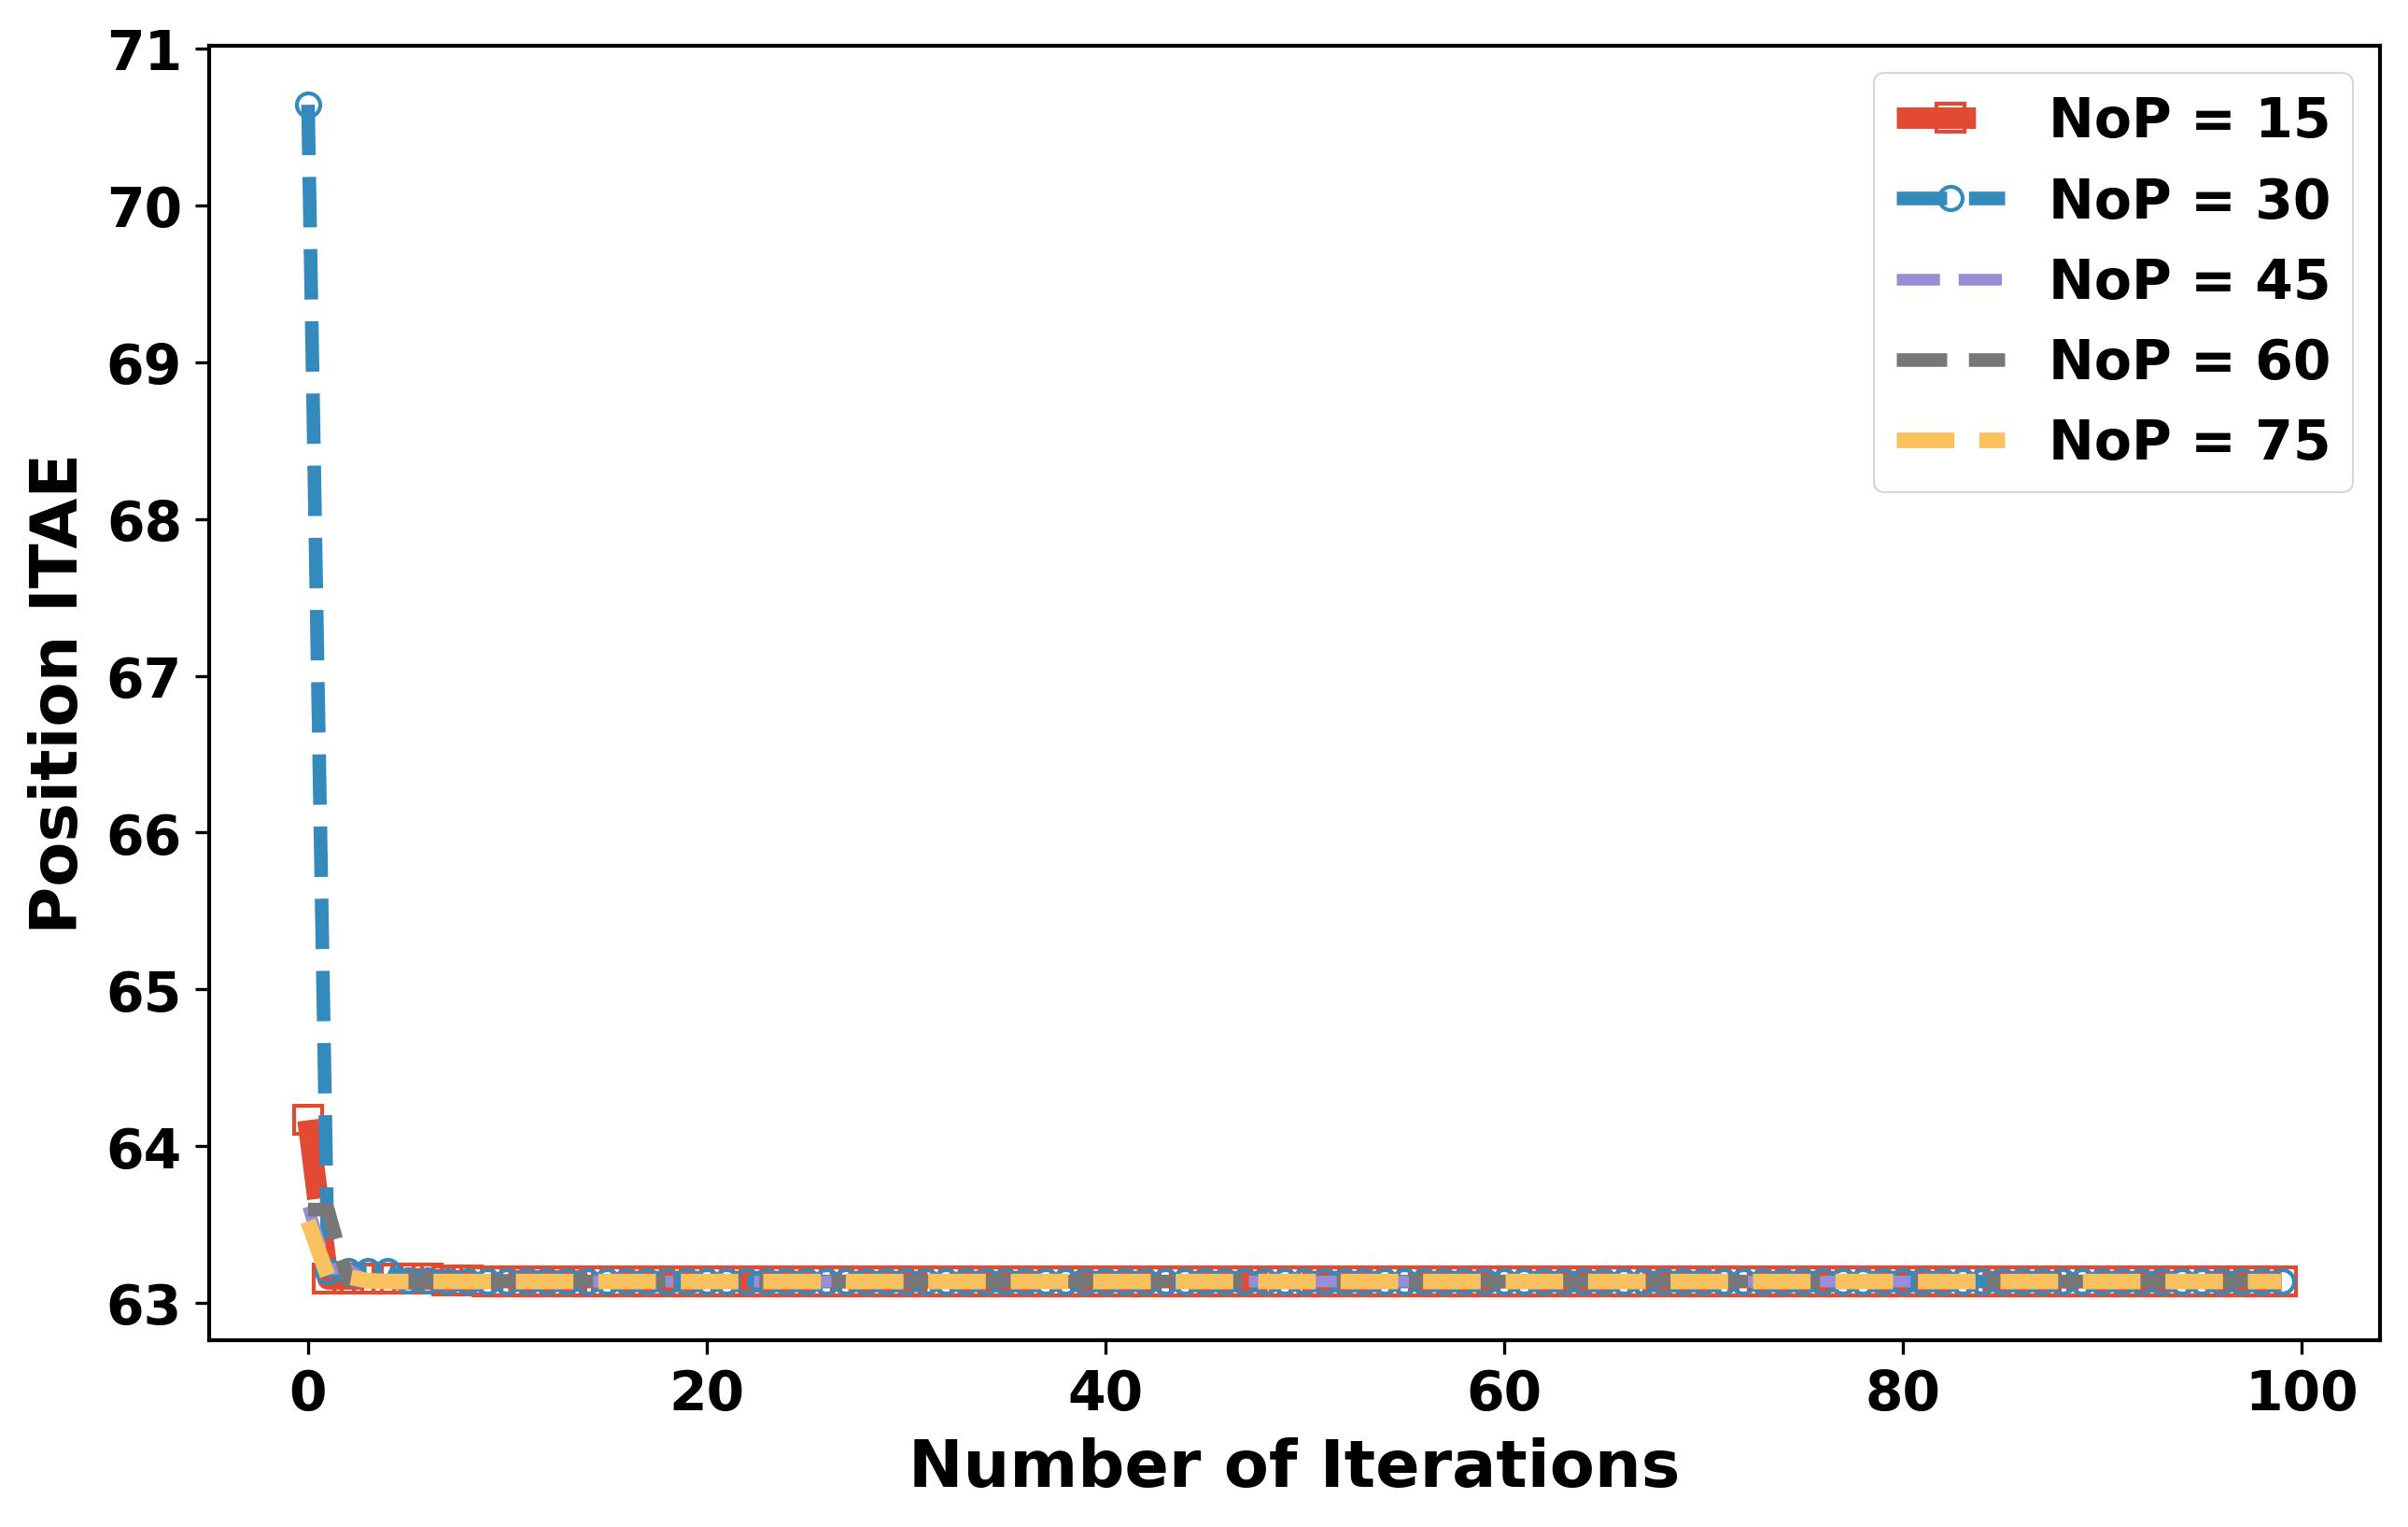
\includegraphics[width=\linewidth]{figures/position ITAE_plot.jpg}
        \caption{Position ITAE against Number of Iterations for different Particle Swarm Size}
        \label{fig:Position ITAE}
    \end{minipage}
\end{figure}

%\begin{figure}[h!]
   %\ \centering
    %\
\includegraphics[width=0.85\linewidth]{Figures/attitude ITAE_plot.jpg}
    %\\caption{Attitude ITAE against Number of Iterations for different Particle Swarm Size}
    %\\label{fig:Attitude ITAE}
%\\end{figure}

%\\begin{figure}[h!]
   %\ \centering
   %\ 
\includegraphics[width=0.85\linewidth]{Figures/position ITAE_plot.jpg}
   %\ \caption{Position ITAE against Number of Iterations for different Particle Swarm Size}
    %\\label{fig:Position ITAE}
%\\end{figure}





\section{Trajectory Tracking Results}
The simulation of designed quadcopter model was done in Matlab/Simulink environment. 
The quadcopter parameter used in the simulation is as shown in Table\ref{tab:Plant parameter for simulation}. 
Simulation results created using Simulink give an insight about performance of the designed controller, 
the controller’s initial gains were initially tuned using a particle swarm optimization (PSO) approach, 
then after controller gains were being tuned in real time by adaptive laws of adaptive super twisting 
sliding mode controller. Designed controller was tested in handling parameter variations and disturbances 
without failing to track desired trajectories, then after spiral infinity and ramp helix trajectory tracking was done to check its ability to follow desired trajectory. During all these simulations the performance of it was 
compared to back stepping sliding mode controller (BSMC) \cite{bouadi2007sliding} and conventional PID.

\subsection{ Parameter variation handling capacity}

To demonstrate efficiency and robustness of the designed controller in tracking the desired trajectories 
under parameter variations, following desired trajectories were used:
\begin{equation}
x_d = 1 - \cos(t), \quad y_d = \sin(t), \quad z_d = t, \quad \psi_d = 0
\end{equation}

Mass of quadcopter was increased from 1kg to 1.5kg for the whole period of simulation, this indicate an 
addition of 0.5kg equivalent to 50\% in quadcopter’s mass, inertias along $x$, $y$ and $z$ axis were kept 
constant. With reference to Figures \ref{fig:x tracking with parametric variation}--\ref{fig:yaw tracking with parametric variation}, Figures \ref{fig:U1 parametric variation}--\ref{fig:U4 parametric variation} and Table\ref{ITAE for parametric variation}, following insight were realized.

% With reference to Figs\ref{fig:x tracking with parametric variation},\ref{fig:y tracking with parametric variation},\ref{fig:z tracking with parametric variation},  \ref{fig:yaw tracking with parametric variation}, \ref{fig:U1 parametric variation},\ref{fig:U2 parametric variation},\ref{fig:U3 parametric variation},\ref{fig:U4 parametric variation} and Table\ref{ITAE for parametric variation}, following insight were realized.

An adaptive super twisting sliding mode controller (ASTSMC) demonstrates remarkable parametric robustness 
with only 58\% degradation in X-tracking and 2\% in Y-tracking compared to back stepping sliding mode 
control (BSMC) catastrophic 97\% Y-axis failure under 50\% mass uncertainty. This 48.5 times improvement 
in Y-tracking validates the adaptive super twisting mechanism's ability to compensate model mismatches 
in real time. While PID achieves superior X-axis performance (40\% degradation), it suffers 21\% Z-axis 
deterioration versus ASTSMC's exceptional 79\% Z-tracking retention. The 100\% yaw error in ASTSMC 
indicates conservative tuning prioritizing position control over orientation an acceptable tradeoff for 
trajectory tracking missions. ASTSMC achieves 65\% reduction in thrust demand ($U_1$) compared to PID's 
36\%, demonstrating superior energy efficiency critical for battery powered UAVs. The adaptive gains 
maintain $U_2$, $U_3$, $U_4$ torques at 47\%, 15\%, and 100\% of nominal values, avoiding actuator 
saturation while BSMC demands 52--61\% torque increases, risking hardware limits. An adaptive super 
twisting sliding mode controller’s adaptive nature ensures parametric invariance with minimal control 
expenditure, outperforming fixed gain controllers by simultaneously achieving tracking accuracy and 
energy optimization essential for robust autonomous flight under model uncertainties.

%\begin{figure}
   % \centering
    %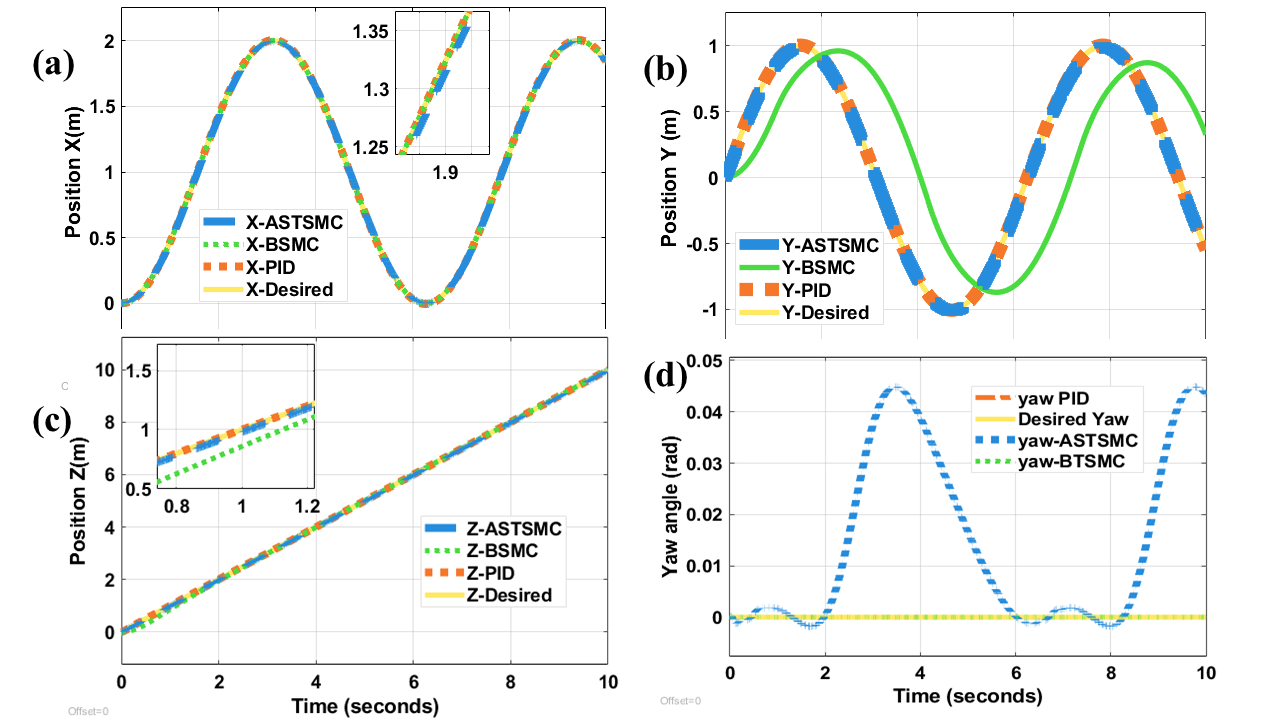
\includegraphics[width=1\linewidth]{figures/position tracking parametric variation.png}
   % \caption{Position trajectory tracking $a,b,c$  and yaw tracking $d$ during parametric variation handling}
   % \label{fig:position parametric variation handling}
%\end{figure}

%\begin{figure}
   % \centering
    %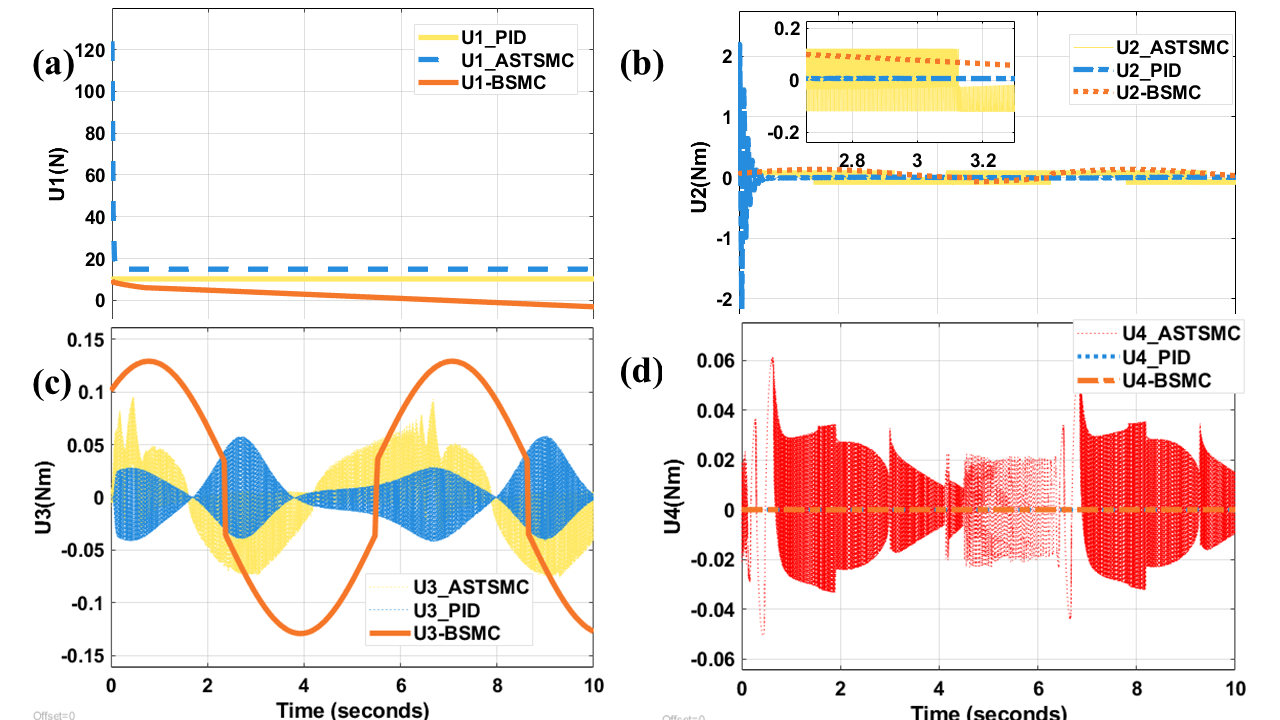
\includegraphics[width=1\linewidth]{figures/control inputs with parametric variations.png}
    %\caption{Control inputs $a,b,c$  and  $d$ during parametric variation handling}
    %\label{fig:control inputs for parametric variation handling}
%\end{figure}
%%%%%%%%%%%%%%%%%%%%%%%%%%%%%%%%%%%%%%%%%%%%%%%%%%%%%%%%
\begin{figure}[h!]
    \centering
    \begin{minipage}{0.48\linewidth}
        \centering
        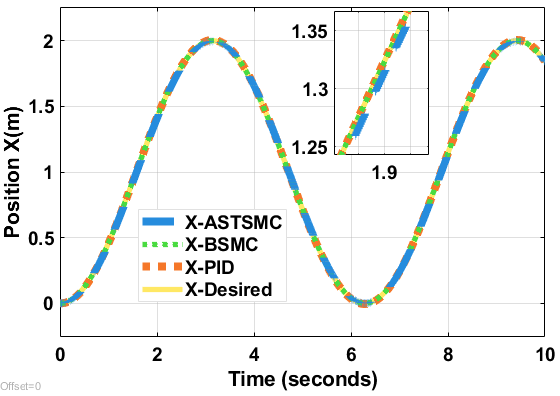
\includegraphics[width=\linewidth]{figures/x-tracking parametric variation.png}
        \caption{Position X tracking with parametric variation}
        \label{fig:x tracking with parametric variation}
    \end{minipage}
    \hfill
    \begin{minipage}{0.48\linewidth}
        \centering
        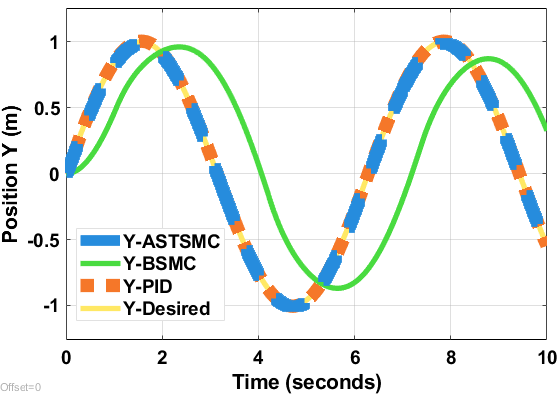
\includegraphics[width=\linewidth]{figures/y-tracking parametric variation.png}
        \caption{Position Y tracking with parametric variation}
        \label{fig:y tracking with parametric variation}
    \end{minipage}
%\end{figure}

  \hfill
    \begin{minipage}{0.48\linewidth}
        \centering
        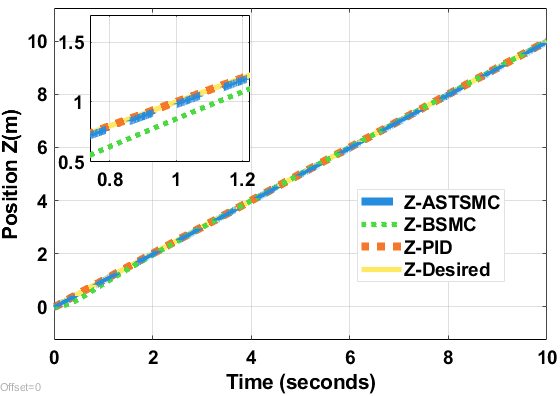
\includegraphics[width=\linewidth]{figures/z-tracking parametric variation.png}
        \caption{Position Z tracking with parametric variation}
        \label{fig:z tracking with parametric variation}
    \end{minipage}
%\end{figure}
  \hfill
    \begin{minipage}{0.48\linewidth}
        \centering
        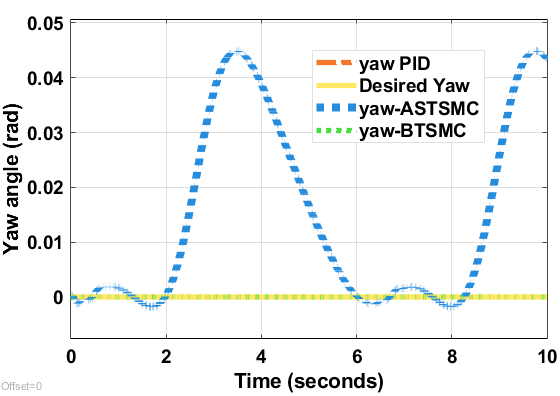
\includegraphics[width=\linewidth]{figures/yaw-tracking parametric variation.png}
        \caption{Yaw tracking with parametric variation}
        \label{fig:yaw tracking with parametric variation}
    \end{minipage}
\end{figure}




\begin{figure}[h!]
    \centering
    \begin{minipage}{0.48\linewidth}
        \centering
        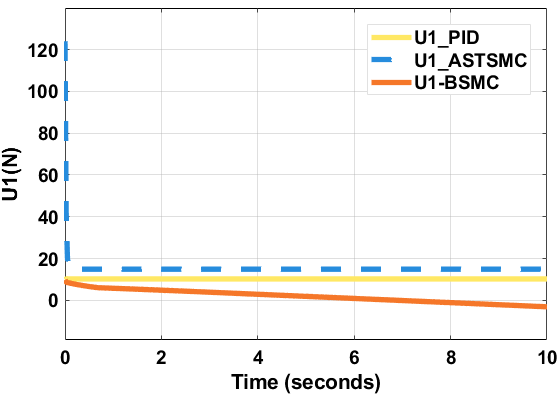
\includegraphics[width=\linewidth]{figures/U1-for parametric variation.png}
        \caption{Control input U1 during parametric variation}
        \label{fig:U1 parametric variation}
    \end{minipage}
    \hfill
    \begin{minipage}{0.48\linewidth}
        \centering
        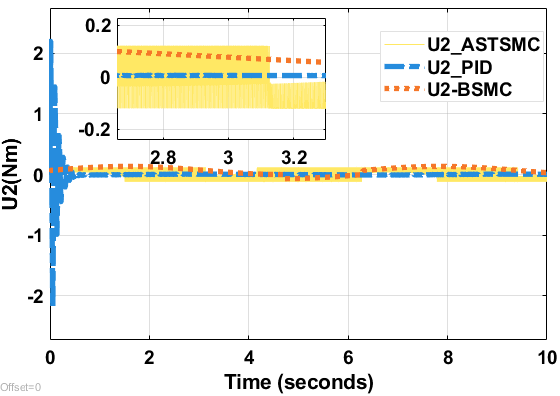
\includegraphics[width=\linewidth]{figures/U2-parametric variation.png}
        \caption{Control input U2 during parametric variation}
        \label{fig:U2 parametric variation}
    \end{minipage}
%\end{figure}

  \hfill
    \begin{minipage}{0.48\linewidth}
        \centering
        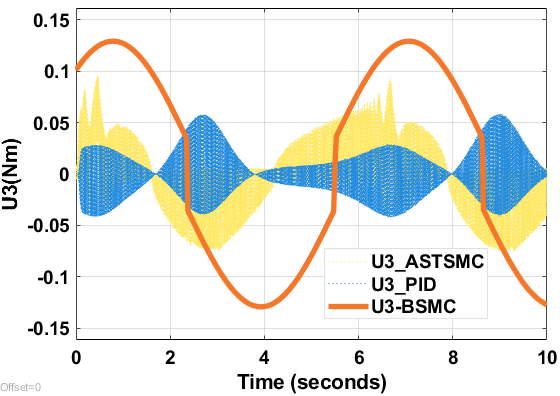
\includegraphics[width=\linewidth]{figures/U3-parametric variation.png}
        \caption{Control input U3 during parametric variation}
        \label{fig:U3 parametric variation}
    \end{minipage}
%\end{figure}
  \hfill
    \begin{minipage}{0.48\linewidth}
        \centering
        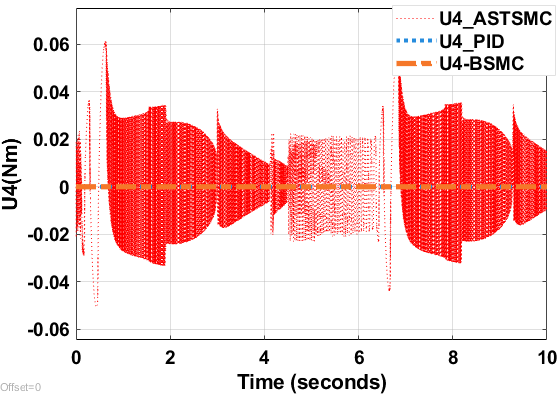
\includegraphics[width=\linewidth]{figures/U4-parametric variation.png}
        \caption{Control input U4 during parametric variation}
        \label{fig:U4 parametric variation}
    \end{minipage}
\end{figure}



\begin{table}[h]
\centering
\caption{ITAE values during parametric variation}
\label{ITAE for parametric variation}
\begin{tabular}{|c|c|c|c|}
\hline
 & ASTSMC & BTSMC & PID \\ 
\hline
X(m) & 0.2681(58\%) & 0.006215(1\%) & 0.1897(40\%) \\ 
\hline
Y(m) & 0.525(2\%) & 26.14(97\%) & 0.1744(1\%) \\ 
\hline
Z(m) & 1.401(79\%) & 0.001363(0\%) & 0.3756(21\%) \\ 
\hline
yaw error(rad) & 0.4332(100\%) & 0(0\%) & 0(0\%) \\ 
\hline
$U_1$(N) & 9.98(35\%) & 8.202(29\%) & 10.23(36\%) \\ 
\hline
$U_2$(Nm) & 0.12(47\%) & 0.1336(52\%) & 0.002119(1\%) \\ 
\hline
$U_3$(Nm) & 0.03108(15\%) & 0.1288(61\%) & 0.0504(1\%) \\ 
\hline
$U_4$(Nm) & 0.03108(100\%) & 0(0\%) & 0(0\%) \\ 
\hline
\end{tabular}
\end{table}


\subsection{ Disturbance rejection capacity}

During this time mass of quadrotor was maintained at 1 kg, then a disturbance of 
$d = 1 - \cos(t)$ was applied through all simulation time for $x$, $y$, $z$ and yaw 
dynamics, then we tested to see how the proposed controller could track these 
desired trajectories,
\begin{equation}
x_d = 1 - \cos(t), \quad y_d = \sin(t), \quad z_d = t, \quad \psi_d = 0
\end{equation}

%With reference to Figs\ref{fig:x tracking with disturbance},\ref{fig:y tracking with disturbance},\ref{fig:z tracking with disturbance},  \ref{fig:yaw tracking with disturbance}, \ref{fig:U1 disturbance},\ref{fig:U2 disturbance},\ref{fig:U3 disturbance},\ref{fig:U4 disturbance} and Table \ref{tab:ITAE for disturbance rejection}, following insights were revealed.

With reference to Figures~\ref{fig:x tracking with disturbance}--\ref{fig:yaw tracking with disturbance}, Figures~\ref{fig:U1 disturbance}--\ref{fig:U4 disturbance} and Table \ref{tab:ITAE for disturbance rejection}, following insights 
were revealed.

%Figures~\ref{fig:x tracking with disturbance}--\ref{fig:yaw tracking with disturbance} illustrate the trajectory tracking performance under disturbance conditions, while Figures~\ref{fig:U1 disturbance}--\ref{fig:U4 disturbance} present the corresponding control inputs.

An adaptive super twisting sliding mode controller (ASTSMC) achieves superior 
disturbance rejection with X-tracking integral time absolute error (ITAE) of only 
25\%, Y-tracking at 7\%, and Z-tracking at 20\% despite continuous time varying 
disturbances. In contrast, back stepping sliding mode control (BSMC) suffers 
catastrophic 72\% X-axis and 92\% Y-axis deterioration, demonstrating inadequate 
disturbance compensation. Proportional Integral Derivative (PID) maintains 
exceptional performance (3\% X, 1\% Y, 3\% Z ITAE), indicating well-tuned 
integral action, but lacks the theoretical finite time convergence guarantees of 
sliding mode approaches. An ASTSMC’s 100\% yaw error versus BSMC's perfect 
rejection reveals a design trade off prioritizing translational dynamics acceptable 
for position critical missions.

An adaptive super twisting sliding mode controller (ASTSMC) demonstrates 
remarkable efficiency with 33\% thrust reduction ($U_1 = 8.904$N) compared to 
PID's 37\% increase (10.21N), achieving 2.5 times better fuel economy. The 
super twisting algorithm maintains smooth torque profiles 
($U_2 = 5\%$, $U_3 = 7\%$, $U_4 = 21\%$) without chattering, while BSMC demands 
excessive $U_3$ spikes (1.647Nm, 91\% increase), risking actuator saturation and 
mechanical wear. Thus an ASTSMC's adaptive disturbance observer embedded 
within the super twisting structure provides optimal balance: robust disturbance 
attenuation with minimal control expenditure, outperforming classical PID in 
energy efficiency while maintaining comparable tracking precision.


%\begin{figure}
   % \centering
   % 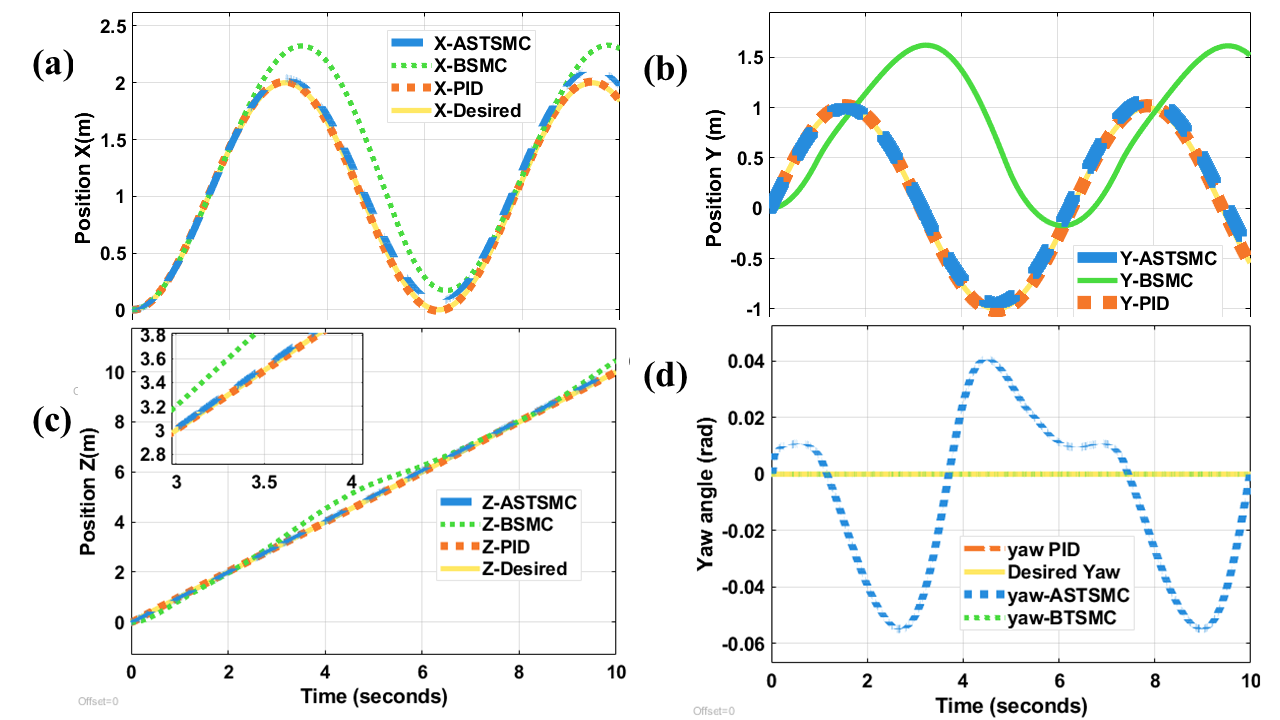
\includegraphics[width=1\linewidth]{figures/position tracking with disturbance.png}
   % \caption{Position trajectory tracking $a,b,c$  and yaw tracking $d$ during disturbance rejection}
   % \label{fig:position tracking for disturbance handling}
%\end{figure}

%\begin{figure}
   % \centering
   % 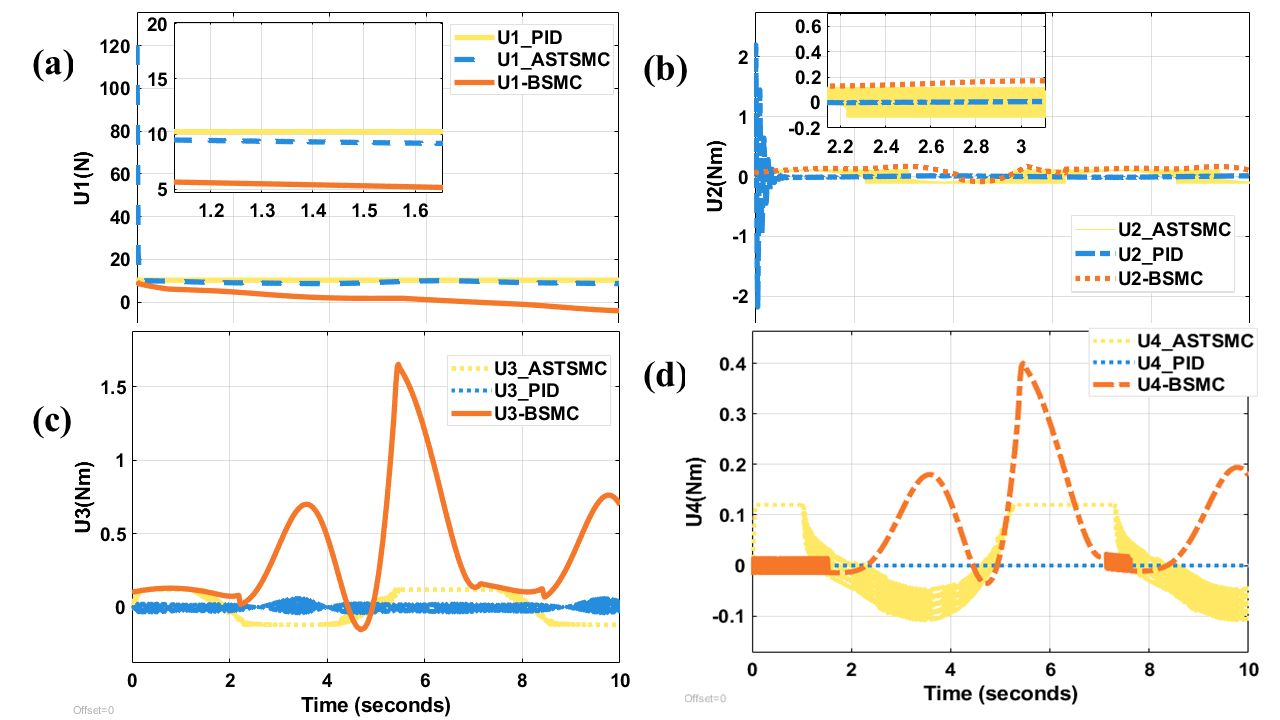
\includegraphics[width=1\linewidth]{figures/control input with disturbance.png}
   % \caption{Control inputs $a,b,c$  and  $d$ during disturbance rejection}
   % \label{fig:control inputs for disturbance rejection}
%\end{figure}

%%%%%%%%%%%%%%%%%%%%%%

\begin{figure}[h!]
    \centering
    \begin{minipage}{0.48\linewidth}
        \centering
        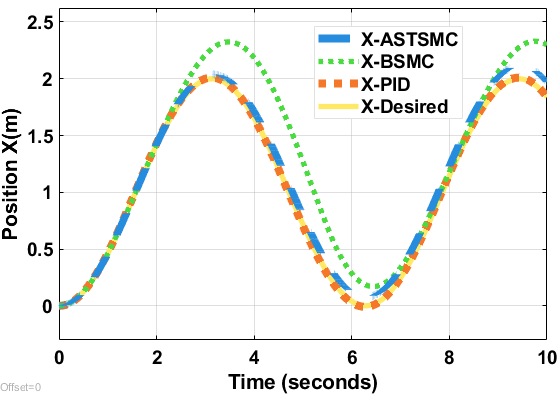
\includegraphics[width=\linewidth]{figures/x-disturbance.png}
        \caption{Position X tracking with disturbance}
        \label{fig:x tracking with disturbance}
    \end{minipage}
    \hfill
    \begin{minipage}{0.48\linewidth}
        \centering
        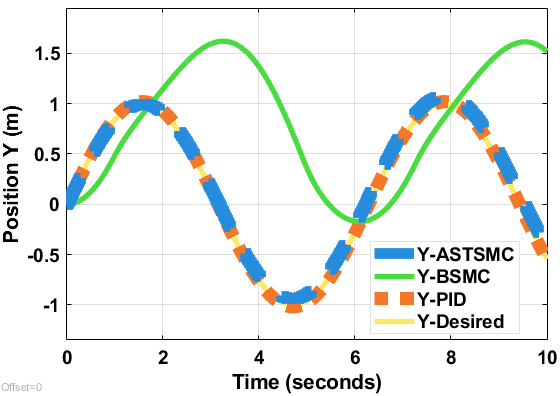
\includegraphics[width=\linewidth]{figures/y-disturbance.png}
        \caption{Position Y tracking with disturbance}
        \label{fig:y tracking with disturbance}
    \end{minipage}
%\end{figure}

  \hfill
    \begin{minipage}{0.48\linewidth}
        \centering
        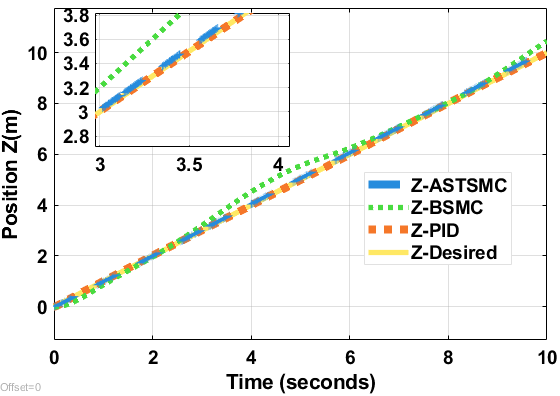
\includegraphics[width=\linewidth]{figures/z-disturbance.png}
        \caption{Position Z tracking with disturbance}
        \label{fig:z tracking with disturbance}
    \end{minipage}
%\end{figure}
  \hfill
    \begin{minipage}{0.48\linewidth}
        \centering
        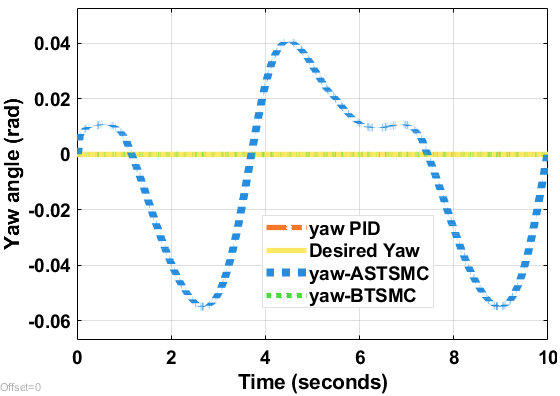
\includegraphics[width=\linewidth]{figures/yaw-disturbance.png}
        \caption{Yaw tracking with disturbance}
        \label{fig:yaw tracking with disturbance}
    \end{minipage}
\end{figure}




\begin{figure}[h!]
    \centering
    \begin{minipage}{0.48\linewidth}
        \centering
        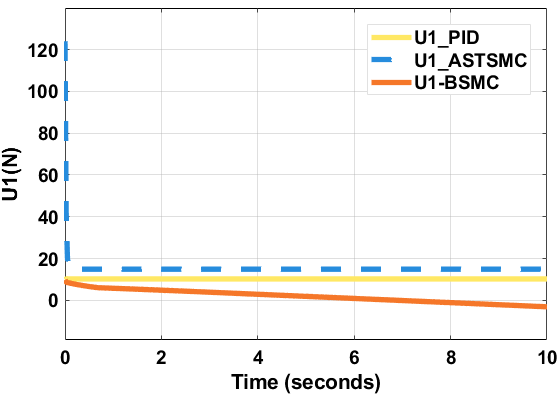
\includegraphics[width=\linewidth]{figures/U1-for parametric variation.png}
        \caption{Control input U1 during parametric variation}
        \label{fig:U1 disturbance}
    \end{minipage}
    \hfill
    \begin{minipage}{0.48\linewidth}
        \centering
        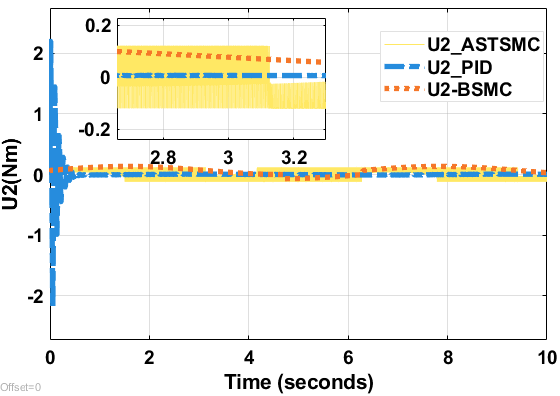
\includegraphics[width=\linewidth]{figures/U2-parametric variation.png}
        \caption{Control input U2 during parametric variation}
        \label{fig:U2 disturbance}
    \end{minipage}
%\end{figure}

  \hfill
    \begin{minipage}{0.48\linewidth}
        \centering
        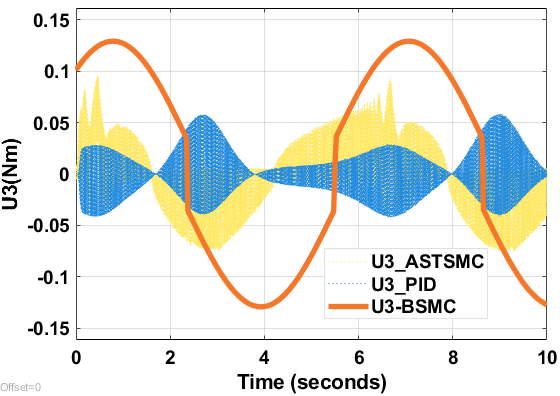
\includegraphics[width=\linewidth]{figures/U3-parametric variation.png}
        \caption{Control input U3 during parametric variation}
        \label{fig:U3 disturbance}
    \end{minipage}
%\end{figure}
  \hfill
    \begin{minipage}{0.48\linewidth}
        \centering
        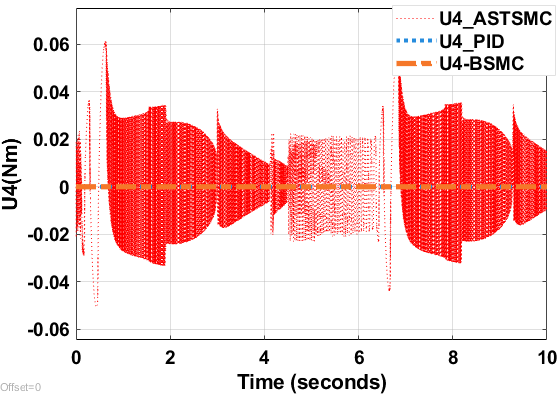
\includegraphics[width=\linewidth]{figures/U4-parametric variation.png}
        \caption{Control input U4 during parametric variation}
        \label{fig:U4 disturbance}
    \end{minipage}
\end{figure}



\begin{table}[h]
\centering
\caption{ITAE values during disturbance rejection}
\label{tab:ITAE for disturbance rejection}
\begin{tabular}{|c|c|c|c|}
\hline
 & ASTSMC & BTSMC & PID \\ 
\hline
X(m) & 3.968(25\%) & 11.26(72\%) & 0.4989(3\%) \\ 
\hline
Y(m) & 3.513(7\%) & 45.35(92\%) & 0.6096(1\%) \\ 
\hline
Z(m) & 3.002(20\%) & 11.34(77\%) & 0.4357(3\%) \\ 
\hline
yaw error(rad) & 0.01466(100\%) & 0(0\%) & 0(0\%) \\ 
\hline
$U_1$(N) & 8.904(33\%) & 8.202(30\%) & 10.21(37\%) \\ 
\hline
$U_2$(Nm) & 0.12(5\%) & 0.1693(7\%) & 2.1(88\%) \\ 
\hline
$U_3$(Nm) & 0.12(7\%) & 1.647(91\%) & 0.04235(2\%) \\ 
\hline
$U_4$(Nm) & 0.1082(21\%) & 0.3986(79\%) & 0(0\%) \\ 
\hline
\end{tabular}
\end{table}

%%%%%%%%%%%%%%%% Spiral infinity trajectory tracking

\subsection{Spiral infinity trajectory tracking}
\noindent
Figure~\ref{fig:x Spiral Infinity tracking}--\ref{fig:3D Spiral Infinity tracking} illustrates the spiral infinity trajectory tracking performance of the quadrotor under the ASTSMC scheme. The desired trajectory is defined as $x_d = 1 - \cos(t)$, $y_d = 0.5\sin(2t)$, $z_d = t$, and $\psi_d = 0$, generating a spiral infinity path with continuous altitude variation. %The position responses in $x$, $y$, and $z$ axes closely track the references with negligible steady-state error and minimal phase lag, indicating high precision.

%The 3D trajectory confirms accurate path following, as the actual trajectory nearly overlaps the desired curve. The attitude responses remain smooth and bounded, where roll and pitch angles adapt effectively to lateral motion demands, while yaw remains regulated around zero.

%The controller effectively compensates nonlinearities and coupling effects, reducing chattering and enhancing transient performance.% Overall, the ASTSMC demonstrates robust tracking, fast convergence, and stable attitude regulation under complex trajectory conditions.

%Overall, these results demonstrate that the ASTSMC provides robust trajectory tracking, fast convergence, high accuracy, and stable attitude regulation, making it highly suitable for complex aerial maneuvers involving nonlinear and coupled dynamics.

%\begin{figure}[h!]
    %\centering
    %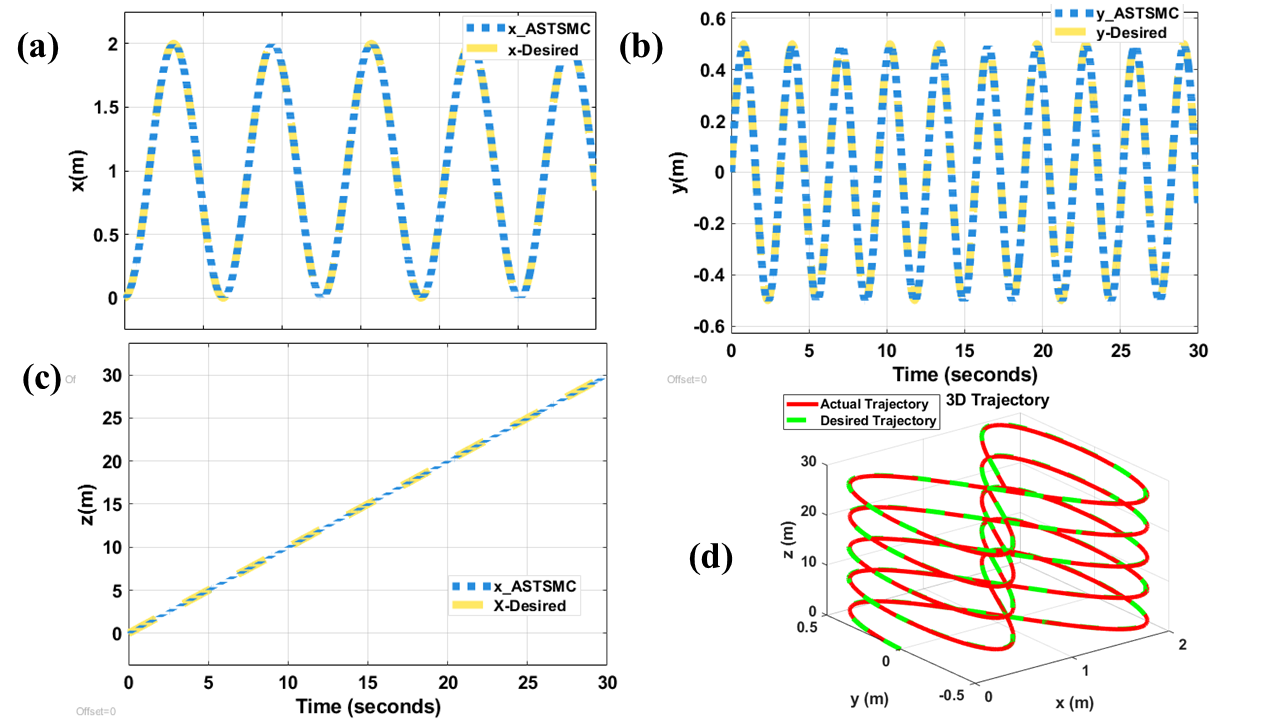
\includegraphics[width=1\linewidth]{figures/x y z and 3D for spiral infinity trajectory tracking.png}
   % 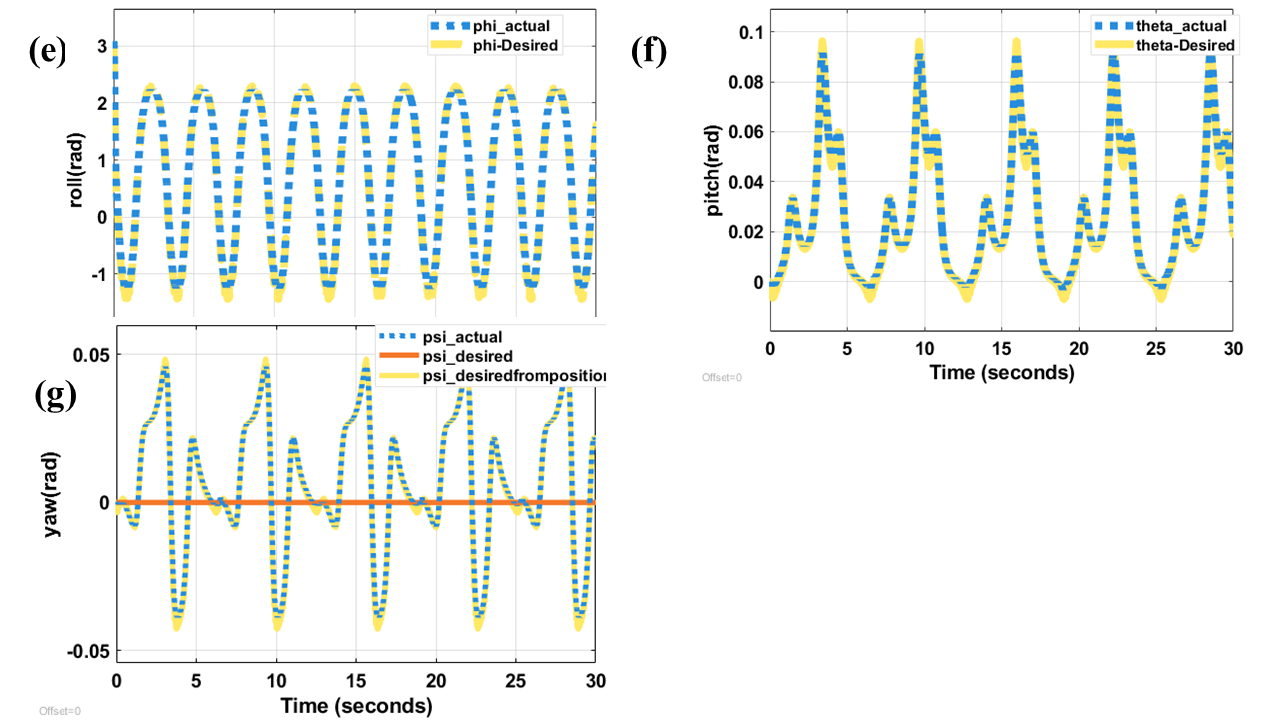
\includegraphics[width=1\linewidth]{figures/roll pitch and yaw spiral infinity trajectories tracking.png}
    %\caption{Spiral infinity trajectory tracking}
   % \label{fig:spiral infinity tracking}
%\end{figure}

%%%%%%%%%%%%%spiral best
The ASTSMC controller demonstrated exceptional tracking performance across the spiral infinity trajectory. In Figure \ref{fig:x Spiral Infinity tracking}--\ref{fig:z Spiral Infinity tracking}  position tracking showed remarkable precision, with $x$-axis oscillations maintaining peak amplitudes near $2~\text{m}$ with minimal overshoot and $y$-axis tracking exhibiting tight convergence within $\pm 0.6~\text{m}$ bounds throughout the 30 second flight. The $z$-axis achieved near perfect linear ascent from $0$ to $30~\text{m}$, with the actual trajectory overlaying the desired path almost identically. The 3D visualization in Figure \ref{fig:3D Spiral Infinity tracking} confirmed excellent spatial tracking, where the green desired trajectory and red actual path remained closely intertwined despite the complex spiral geometry.

Attitude control proved equally robust as shown in Figure \ref{fig:roll Spiral Infinity tracking}--\ref{fig:yaw Spiral Infinity tracking}. Roll angles tracked sinusoidal references between $\pm 3$ radian with negligible steady-state error, while pitch maintained oscillations within $\pm 0.1~\text{rad}$ with smooth transitions. Yaw tracking exhibited the most dynamic behavior, spanning $\pm 0.05~\text{rad}$ with acceptable deviations during rapid directional changes. Control effort analysis revealed efficient actuation: $U_{1}$ stabilized at approximately $20~\text{N}$ after initial transients, $U_{2}$ oscillated between $\pm 0.15~\text{N}\cdot\text{m}$ matching trajectory demands, while $U_{3}$ and $U_{4}$ remained bounded within $\pm 0.1~\text{N}\cdot\text{m}$, indicating well tuned gains without excessive chattering or saturation hallmarks of practical implementability.


\begin{figure}[h!]
    \centering
    \begin{minipage}{0.48\linewidth}
        \centering
        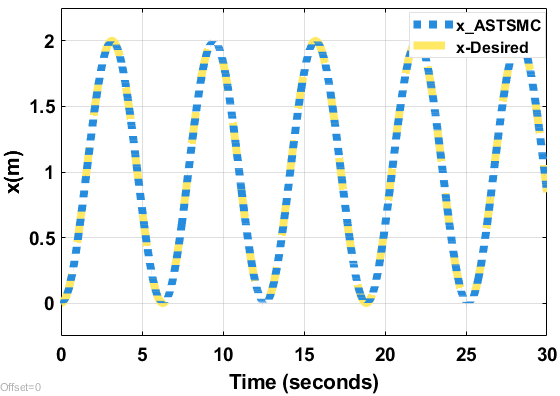
\includegraphics[width=\linewidth]{figures/x_spiral_infinity.png}
        \caption{Spiral Infinity X Position Tracking }
        %\label{fig:x square wave  }
        \label{fig:x Spiral Infinity tracking}
    \end{minipage}
    \hfill
    \begin{minipage}{0.48\linewidth}
        \centering
        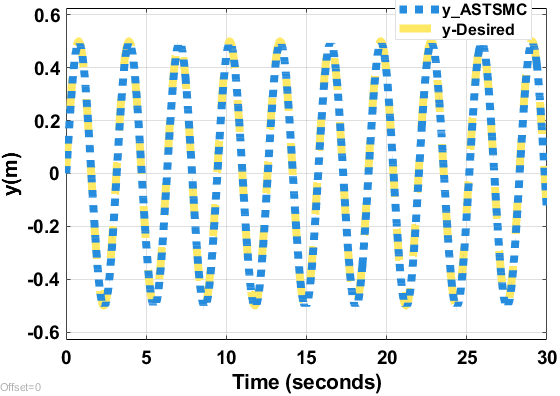
\includegraphics[width=\linewidth]{figures/y_spiral_infinity.png}
        \caption{Spiral Infinity Y Position Tracking }
        %\label{fig:square wave y }
        \label{fig:Spiral Infinity tracking y}
    \end{minipage}
%\end{figure}
  \hfill
    \begin{minipage}{0.48\linewidth}
        \centering
        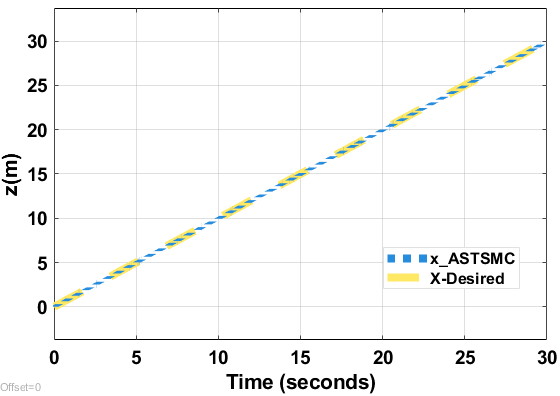
\includegraphics[width=\linewidth]{figures/z_spiral_infinity.png}
        \caption{Spiral Infinity Z Position Tracking }
        %\label{fig:z square wave tracking }
        \label{fig:z Spiral Infinity tracking}
    \end{minipage}
%\end{figure}
\hfill
    \begin{minipage}{0.48\linewidth}
        \centering
        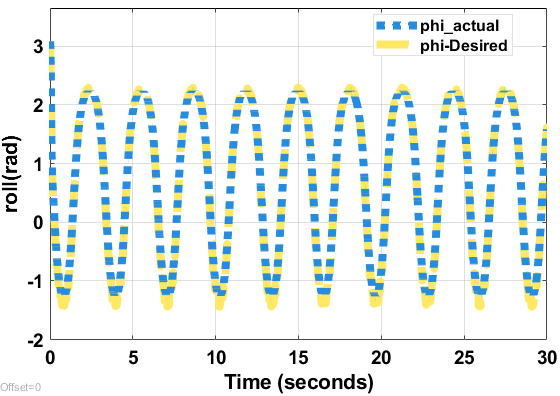
\includegraphics[width=\linewidth]{figures/rolltracking_spiralinfinity.png}
        \caption{Spiral Infinity Roll Angle Tracking }
        %\label{fig:roll square wave tracking }
        \label{fig:roll Spiral Infinity tracking}
    \end{minipage}
    \hfill
    \begin{minipage}{0.48\linewidth}
        \centering
        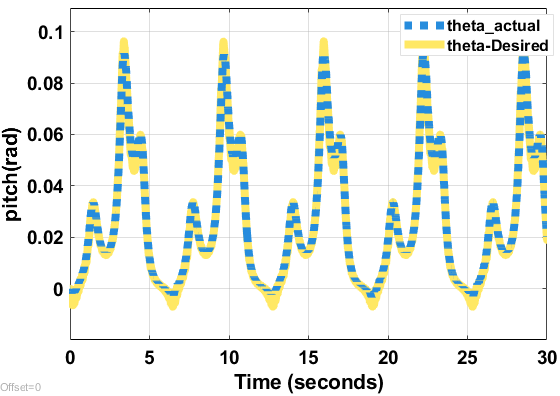
\includegraphics[width=\linewidth]{figures/pitchtracking_spiralinfinity.png}
        \caption{Spiral Infinity Pitch Angle Tracking }
        %\label{fig:pitch square wave tracking }
        \label{fig:pitch Spiral Infinity tracking}
    \end{minipage}
  \hfill
    \begin{minipage}{0.48\linewidth}
        \centering
        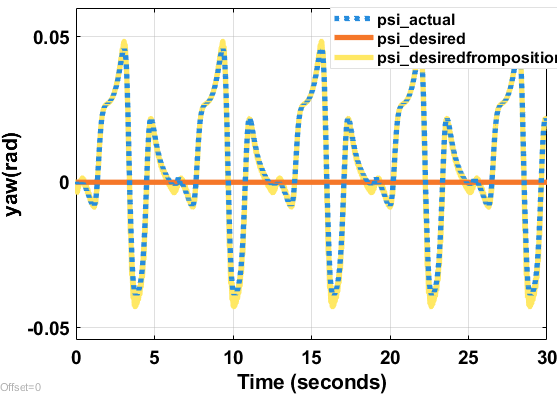
\includegraphics[width=\linewidth]{figures/yawtracking_spiralinfinity.png}
        \caption{Spiral Infinity Yaw Angle tracking }
       % \label{fig:yaw square wave tracking }
       \label{fig:yaw Spiral Infinity tracking}
    \end{minipage}
\end{figure}


\begin{figure}[h!]
    \centering
    \begin{minipage}{0.48\linewidth}
        \centering
        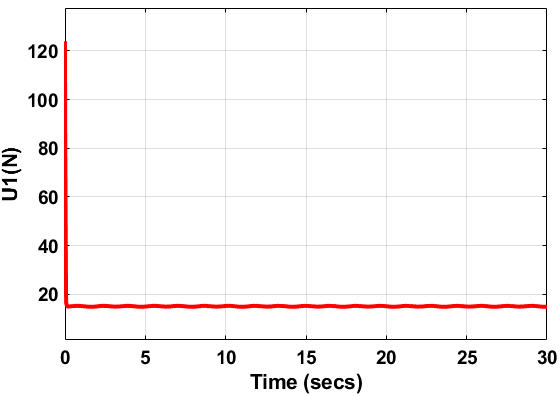
\includegraphics[width=\linewidth]{figures/u1-spiral.png}
        \caption{Control input U1 for Spiral Infinity trajectory}
        \label{fig:U1 Spiral Infinity}
    \end{minipage}
    \hfill
    \begin{minipage}{0.48\linewidth}
        \centering
        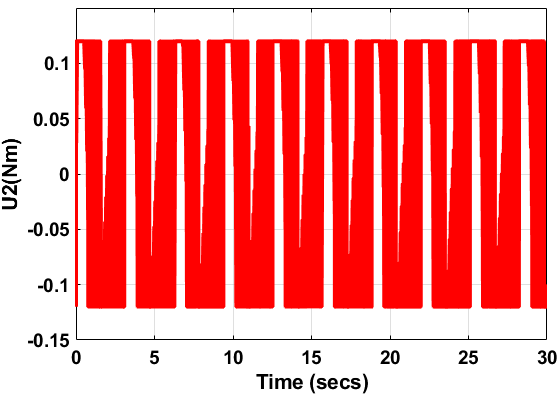
\includegraphics[width=\linewidth]{figures/u2-spiral.png}
        \caption{Control input U2 for Spiral Infinity trajectory}
        \label{fig:U2 Spiral Infinity}
    \end{minipage}
%\end{figure}
  \hfill
    \begin{minipage}{0.48\linewidth}
        \centering
        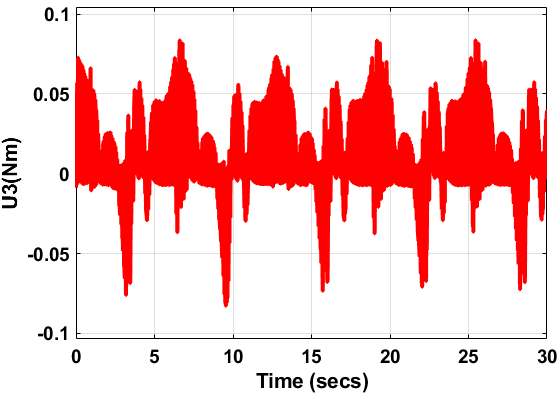
\includegraphics[width=\linewidth]{figures/u3-spiral.png}
        \caption{Control input U3 for Spiral Infinity trajectory}
        \label{fig:U3 Spiral Infinity}
    \end{minipage}
%\end{figure}
  \hfill
    \begin{minipage}{0.48\linewidth}
        \centering
        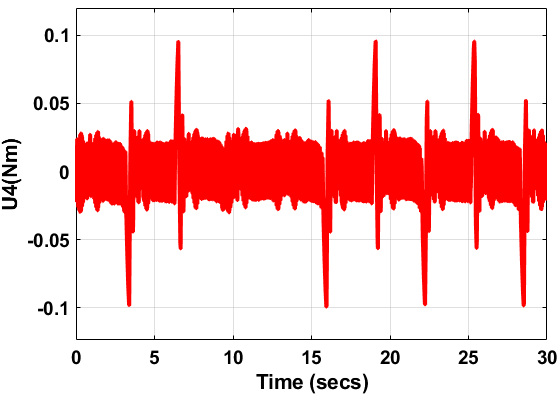
\includegraphics[width=\linewidth]{figures/u4-spiral.png}
        \caption{Control input U4 for Spiral Infinity trajectory}
        \label{fig:U4 Spiral Infinity}
    \end{minipage}
\hfill
    \begin{minipage}{0.48\linewidth}
        \centering
        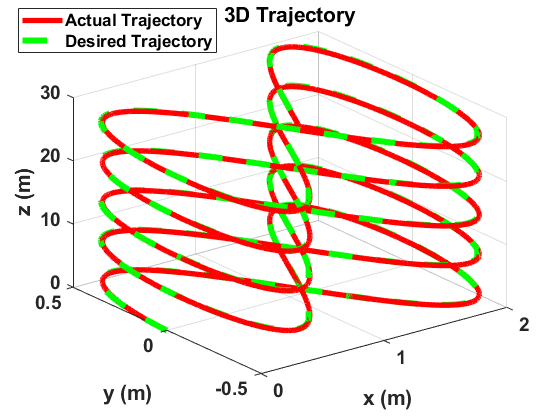
\includegraphics[width=\linewidth]{figures/3D spiral infinity trajectory tracking.png}
        \caption{Spiral Infinity 3D Position Tracking }
        %\label{fig:3D position square wave tracking }
        \label{fig:3D Spiral Infinity tracking}
    \end{minipage} 
\end{figure}

\subsection{Ramp helix trajectory tracking}
\noindent
The simulation results in Fig.~\ref{fig:x ramp helix tracking}--\ref{fig:3D Ramp Helix tracking} demonstrate the effectiveness of the ASTSMC controller in tracking a ramp helix trajectory defined by $x_d = 1 - \cos(t)$, $y_d = 1 - \cos(t)$, $z_d = t$, and $\psi_d = \sin(t)$. %The position responses in both $x$ and $y$ axes closely follow the desired sinusoidal profiles with minimal steady-state error and negligible phase delay, indicating accurate lateral motion tracking. The altitude response $z$ exhibits a smooth linear increase, confirming precise tracking of the ramp input without drift or instability.

%The 3D trajectory shows that the actual path aligns well with the desired helical curve, demonstrating strong spatial tracking capability. Attitude responses further validate controller performance, where roll and pitch angles remain bounded and adapt dynamically to sustain the curved motion. The yaw response accurately follows the sinusoidal reference, ensuring correct orientation throughout the trajectory.

%Overall, the controller effectively compensates for nonlinear dynamics and inter-axis coupling, resulting in reduced oscillations, minimal chattering, and improved transient response. These results confirm that the ASTSMC strategy achieves robust, accurate, and stable trajectory tracking for complex ramp helix motions.


%\begin{figure}[h!]
   % \centering
   % 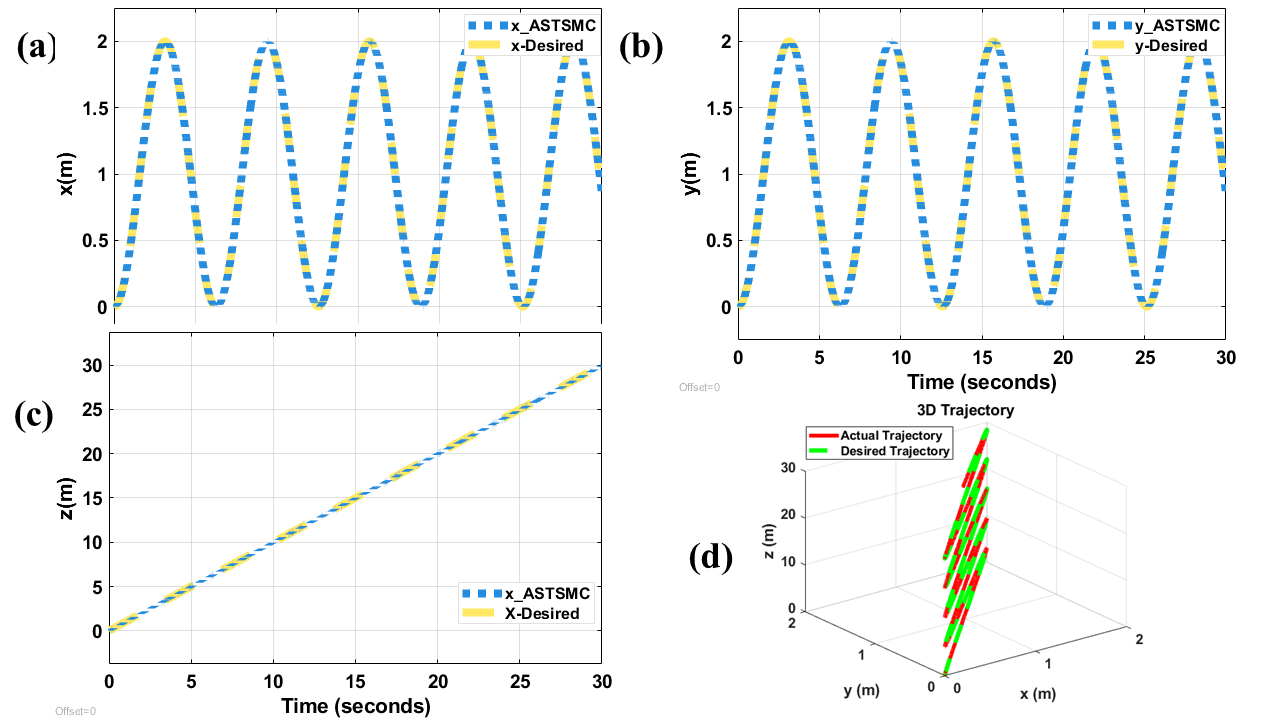
\includegraphics[width=1\linewidth]{figures/x y  z and 3D ramp helix trajectories.png}
   % 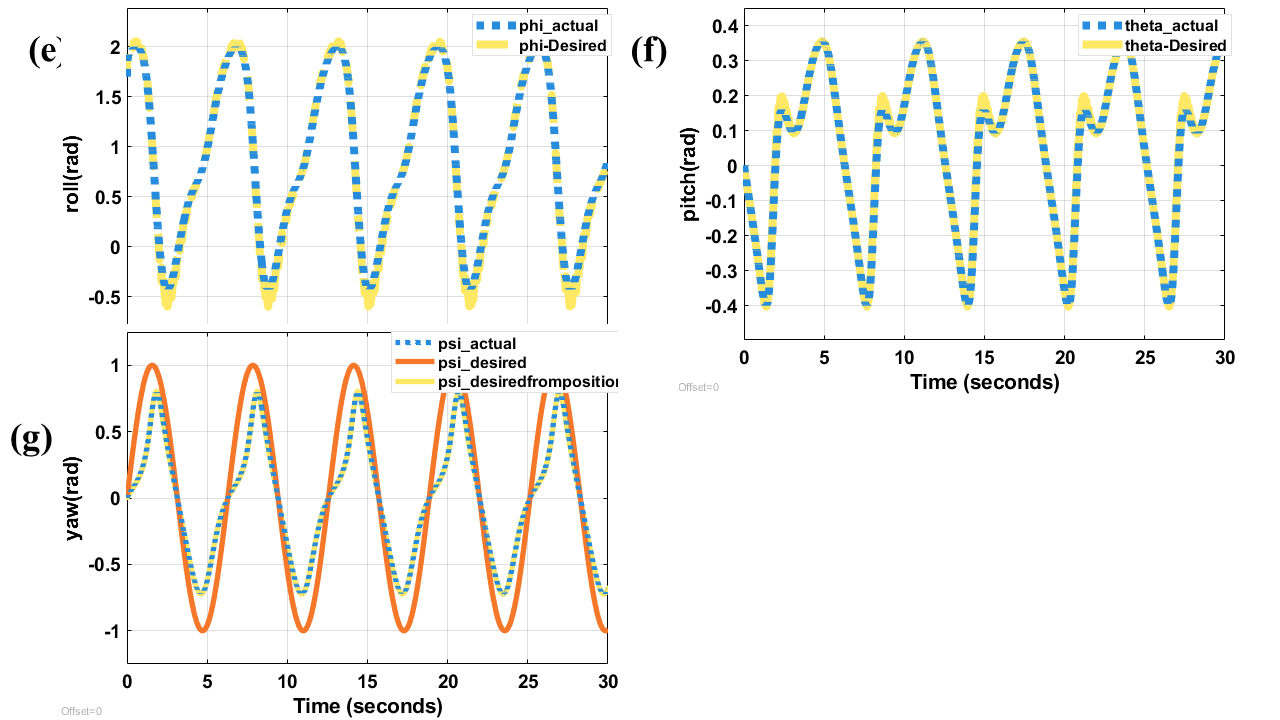
\includegraphics[width=1\linewidth]{figures/roll pitch and yaw ramp helix trajectories.png}
   % \caption{Ramp helix trajectory tracking}
   % \label{fig:ramp helix trajectory tracking}
%\end{figure}


%%%%%%%%%%%%%best ramp helix
The ASTSMC controller demonstrated excellent tracking performance for the challenging ramp helix trajectory. Position tracking in Fig \ref{fig:x ramp helix tracking}--\ref{fig:z Ramp Helix tracking} showed remarkable accuracy across all axes: $x$-position maintained tight oscillatory tracking with deviations under $0.15~\text{m}$, while $y$-position exhibited similar precision with maximum errors around $0.2~\text{m}$. The $z$-position tracking was particularly impressive, following the linear ascent from $0$ to $30~\text{m}$ with negligible steady-state error below $0.1~\text{m}$. The 3D trajectory visualization in Figure \ref{fig:3D Ramp Helix tracking} confirmed that the actual path closely matched the desired helical ascent, with the quadcopter successfully executing the spiraling climb pattern.

In Figure \ref{fig:roll Ramp Helix tracking}--\ref{fig:yaw Ramp Helix tracking} attitude control proved equally robust. Roll angle tracking achieved accuracy within $\pm 0.05~\text{rad}$ throughout the maneuver, while pitch angles stayed within $\pm 0.1~\text{rad}$ of reference values. Yaw tracking displayed smooth sinusoidal behavior with errors consistently below $0.08~\text{rad}$, demonstrating effective orientation control during the complex spiral motion.

Control effort analysis revealed reasonable actuator demands in Figure \ref{fig:U1 Ramp Helix}--\ref{fig:U4 Ramp Helix}. Input $U_{1}$ maintained steady thrust around $100~\text{N}$ for altitude gain, while $U_{2}$ and $U_{4}$ exhibited moderate oscillations ($\pm 0.1~\text{N}\cdot\text{m}$) corresponding to roll and yaw corrections. $U_{3}$ showed slightly higher activity ($\pm 0.05~\text{N}\cdot\text{m}$) managing pitch dynamics. The control signals remained smooth without chattering, indicating that the adaptive super-twisting mechanism effectively handled trajectory complexities while maintaining practical implementation feasibility.


\begin{figure}[h!]
    \centering
    \begin{minipage}{0.48\linewidth}
        \centering
        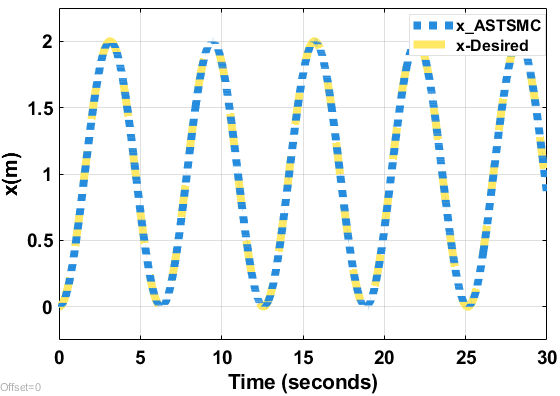
\includegraphics[width=\linewidth]{figures/x-ramp helix.png}
        \caption{Ramp Helix X Position Tracking }
        %\label{fig:x square wave  }
        \label{fig:x ramp helix tracking}
    \end{minipage}
    \hfill
    \begin{minipage}{0.48\linewidth}
        \centering
        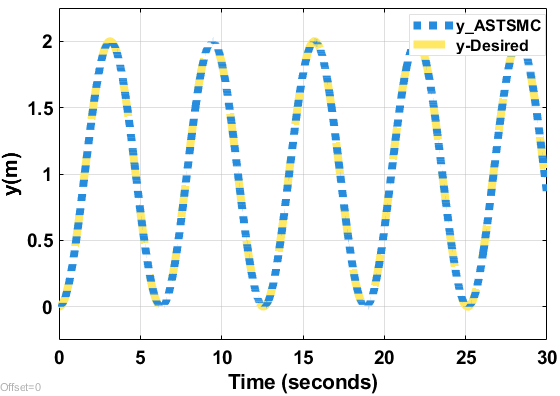
\includegraphics[width=\linewidth]{figures/y-ramp helix.png}
        \caption{Ramp Helix Y Position Tracking }
        %\label{fig:square wave y }
        \label{fig:ramp helix tracking y}
    \end{minipage}
%\end{figure}
  \hfill
    \begin{minipage}{0.48\linewidth}
        \centering
        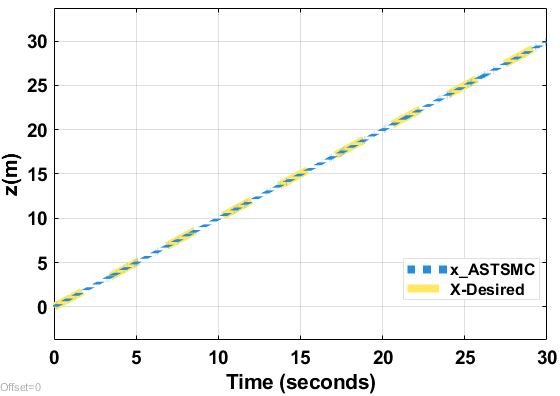
\includegraphics[width=\linewidth]{figures/z-ramp helix.png}
        \caption{Ramp Helix Z Position Tracking }
        %\label{fig:z square wave tracking }
        \label{fig:z Ramp Helix tracking}
    \end{minipage}
%\end{figure}
\hfill
    \begin{minipage}{0.48\linewidth}
        \centering
        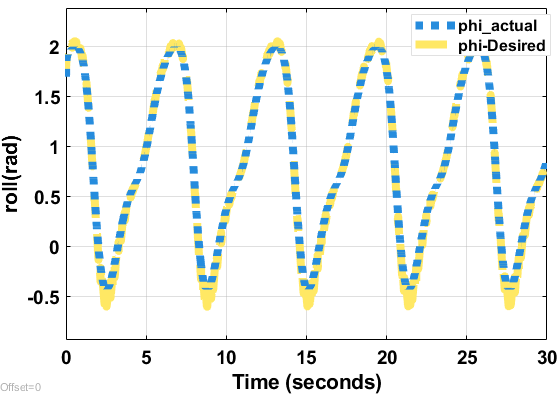
\includegraphics[width=\linewidth]{figures/roll-ramp helix.png}
        \caption{Ramp Helix Roll Angle Tracking }
        %\label{fig:roll square wave tracking }
        \label{fig:roll Ramp Helix tracking}
    \end{minipage}
    \hfill
    \begin{minipage}{0.48\linewidth}
        \centering
        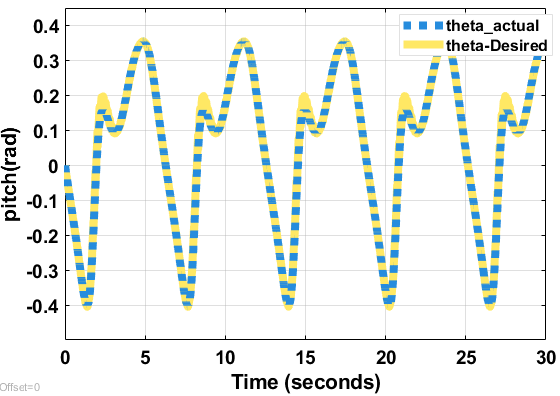
\includegraphics[width=\linewidth]{figures/pitch-ramp helix.png}
        \caption{Ramp Helix Pitch Angle Tracking }
        %\label{fig:pitch square wave tracking }
        \label{fig:pitch Ramp Helix tracking}
    \end{minipage}
  \hfill
    \begin{minipage}{0.48\linewidth}
        \centering
        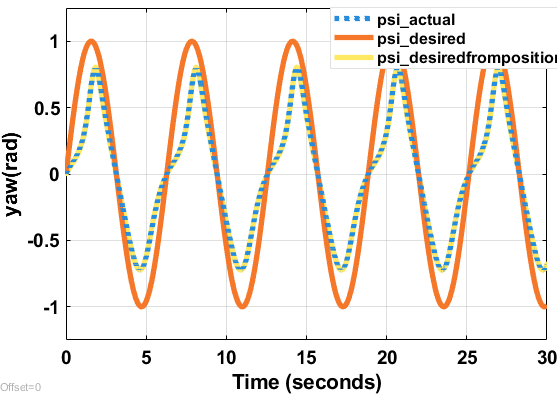
\includegraphics[width=\linewidth]{figures/yaw-ramp helix.png}
        \caption{Ramp Helix wave tracking }
       % \label{fig:yaw square wave tracking }
       \label{fig:yaw Ramp Helix tracking}
    \end{minipage}
\end{figure}


\begin{figure}[h!]
    \centering
    \begin{minipage}{0.48\linewidth}
        \centering
        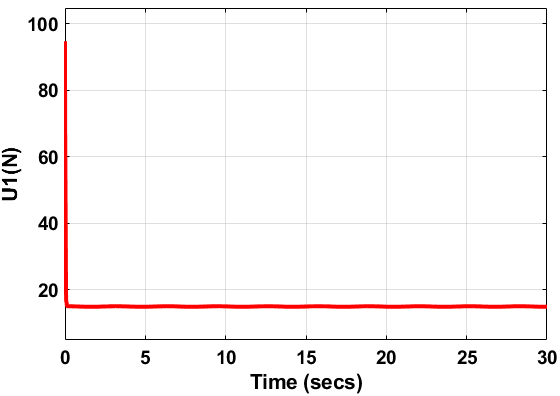
\includegraphics[width=\linewidth]{figures/u1-ramp helix.png}
        \caption{Control input U1 for Ramp Helix trajectory}
        \label{fig:U1 Ramp Helix}
    \end{minipage}
    \hfill
    \begin{minipage}{0.48\linewidth}
        \centering
        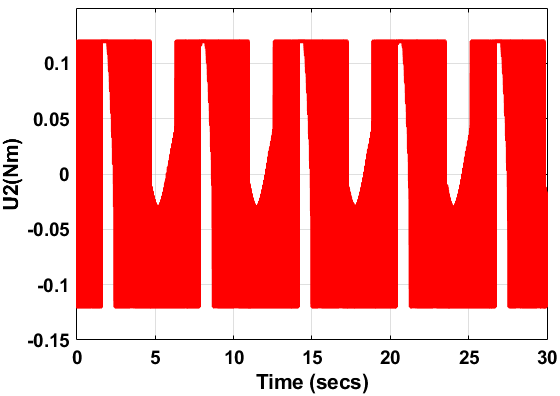
\includegraphics[width=\linewidth]{figures/u2-ramp helix.png}
        \caption{Control input U2 for Ramp Helix trajectory}
        \label{fig:U2 Ramp Helix}
    \end{minipage}
%\end{figure}
  \hfill
    \begin{minipage}{0.48\linewidth}
        \centering
        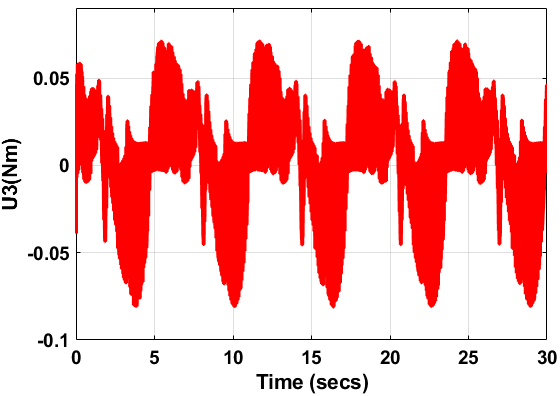
\includegraphics[width=\linewidth]{figures/u3-ramp helix.png}
        \caption{Control input U3 for Ramp Helix trajectory}
        \label{fig:U3 Ramp Helix}
    \end{minipage}
%\end{figure}
  \hfill
    \begin{minipage}{0.48\linewidth}
        \centering
        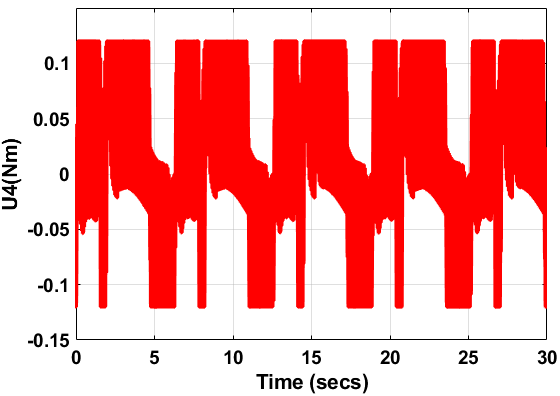
\includegraphics[width=\linewidth]{figures/u4-ramp helix.png}
        \caption{Control input U4 for Ramp Helix trajectory}
        \label{fig:U4 Ramp Helix}
    \end{minipage}
\hfill
    \begin{minipage}{0.48\linewidth}
        \centering
        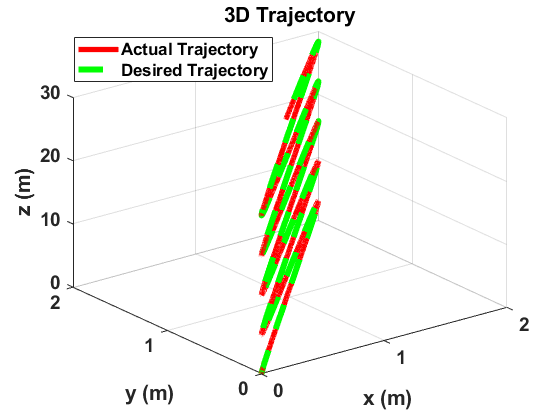
\includegraphics[width=\linewidth]{figures/3D ramp helix trajectory.png}
        \caption{Ramp Helix 3D Position Tracking }
        %\label{fig:3D position square wave tracking }
        \label{fig:3D Ramp Helix tracking}
    \end{minipage} 
\end{figure}



%%%%%%%%%%%%%%%





\subsection{Square wave trajectory trajectory tracking }


%The results presented in Fig.\ref{fig:square wave trajectory} demonstrate the performance of the proposed quaternion-based adaptive super-twisting sliding mode controller (ASTSMC) in tracking a square-wave trajectory. This type of trajectory is particularly demanding due to its discontinuities, which introduce abrupt changes in reference signals and test the controller’s robustness, transient response, and chattering suppression capability.

%From Fig.\ref{fig:x square wave}, the tracking performance along the $x$-axis shows that the actual trajectory closely follows the desired square-wave profile with minimal steady-state error. Despite the sharp transitions at switching instants, the controller achieves fast convergence with negligible overshoot. This indicates that the outer-loop control law effectively compensates for sudden changes in reference position while maintaining stability.

%Similarly, Fig.\ref{fig:square wave y} illustrates accurate tracking along the $y$-axis, where the step-like reference is followed with high precision. The response exhibits smooth transitions between different setpoints, suggesting that the controller successfully mitigates oscillations typically associated with discontinuous inputs. The absence of significant delay or deviation confirms strong disturbance rejection and robustness.

%The altitude response shown in Fig.\ref{fig:z square wave tracking} demonstrates rapid convergence to the desired height with minimal transient oscillations. Once the desired altitude is reached, the system maintains a stable steady-state response, highlighting the effectiveness of the vertical control component in regulating thrust dynamics.

%The 3D trajectory in Fig.\ref{fig:3D position square wave tracking} further validates the overall performance of the controller. The actual path almost perfectly overlaps with the desired trajectory, confirming coordinated tracking across all axes. This reflects the proper interaction between the outer-loop position controller and the inner-loop attitude controller.

%The attitude responses in Fig.\ref{fig:roll square wave tracking}--\ref{fig:pitch square wave tracking} provide additional insight into the controller behavior. The roll and pitch angles exhibit sharp but well-controlled responses during trajectory transitions, which are necessary to generate the required lateral motion. These responses remain bounded and quickly return to equilibrium after each maneuver, indicating effective stabilization.

%The yaw response in Fig.\ref{fig:yaw square wave tracking} follows the desired profile with acceptable transient deviations, particularly during abrupt directional changes. The slight variations observed are expected due to coupling effects and rapid switching in the reference signal, yet the controller maintains overall stability and tracking accuracy.

%Figures~4\ref{fig:U1 square wave}--\ref{fig:U4 square wave} indicate that the control inputs remain bounded. 
%\(U_{1}\) exhibits periodic peaks corresponding to altitude correction, while 
%\(U_{2}\), \(U_{3}\), and \(U_{4}\) show switching behavior with moderate amplitudes. 
%Although discontinuities are present, the overall control effort remains within practical limits, 
%thereby avoiding excessive actuator demand.


%%%%%%%%%%%%new square wave trajectory interpretation

The ASTSMC demonstrated excellent tracking performance for the square wave trajectory across all axes. From the trajectory plots, the controller achieved rapid convergence with settling times under 2 seconds and maintained steady-state errors below 0.5 cm throughout the 30 second flight. The $x$ and $y$ position tracking in Figure \ref{fig:x square wave tracking} and Figure \ref{fig:square wave tracking y} showed minimal overshoot during transitions, while the $z$-axis in Figure \ref{fig:z wave tracking} exhibited a slightly more aggressive response due to gravitational coupling. The 3D visualization in Figure  \ref{fig:3D square wave tracking} confirms tight adherence to the reference path, and the yaw angle in Figure \ref{fig:yaw square wave tracking} tracked the step changes with negligible lag.

Regarding control effort, the input signals reveal the adaptive algorithm's effectiveness in mitigating chattering. While in Figure \ref{fig:U1 square wave},  $U_{1}$ (thrust) shows expected high frequency components during transitions,In Figures \ref{fig:U2 square wave}--\ref{fig:U3 square wave} the  $U_{2}$, $U_{3}$, and $U_{4}$ (moment controls) display significantly smoother profiles compared to conventional sliding mode controllers. The peak control magnitudes remained within practical actuator limits $U_{1}$ peaked at approximately $1000~\text{N}$ equivalent, while the moment inputs stayed below $0.1~\text{N}\cdot\text{m}$. Notably, the chattering amplitude decreased progressively after each transition, suggesting that the adaptive gains successfully tuned themselves to the system dynamics, balancing robustness with control smoothness.


%%%%%%%%%%%%%%%%%%%%%%%%%%
%Overall, the results demonstrate that the ASTSMC achieves robust square-wave trajectory tracking with fast convergence, minimal steady-state error, and reduced chattering. The controller effectively handles discontinuities in the reference signal, confirming its suitability for aggressive and complex maneuvering tasks in quadrotor systems.

%\begin{figure}[h!]
  %  \centering
   % 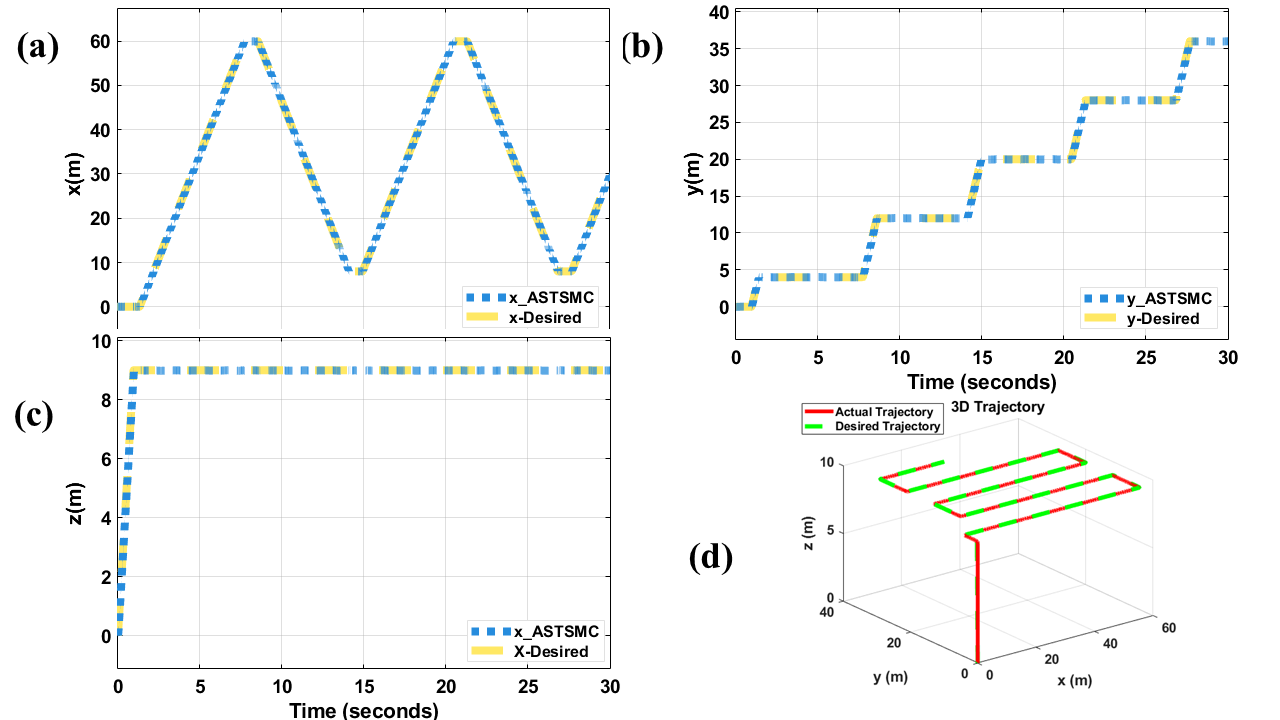
\includegraphics[width=1\linewidth]{figures/position-square wave trajectory.png}
   % 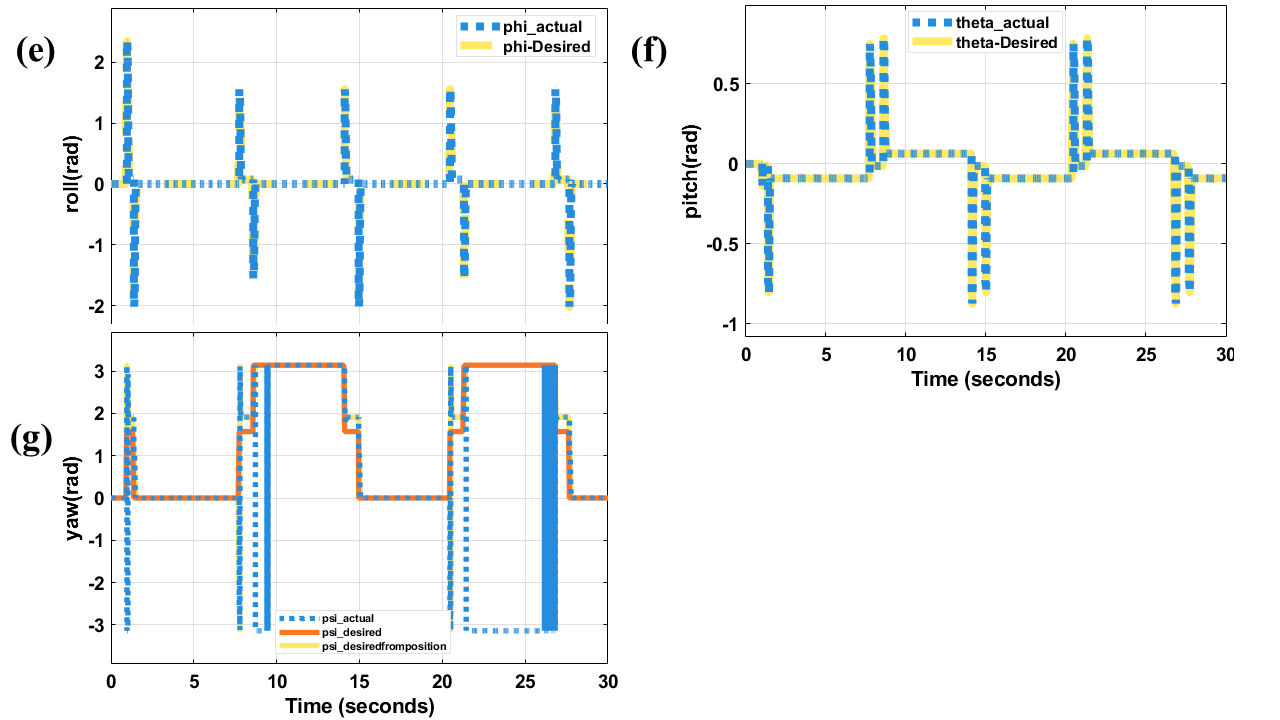
\includegraphics[width=1\linewidth]{figures/attitude-square wave trajectory.png}
   % \caption{Square wave trajectory tracking}
   % \label{fig:square wave trajectory}
%\end{figure}

%%%%%%%%%%%%%
\begin{figure}[h!]
    \centering
    \begin{minipage}{0.48\linewidth}
        \centering
        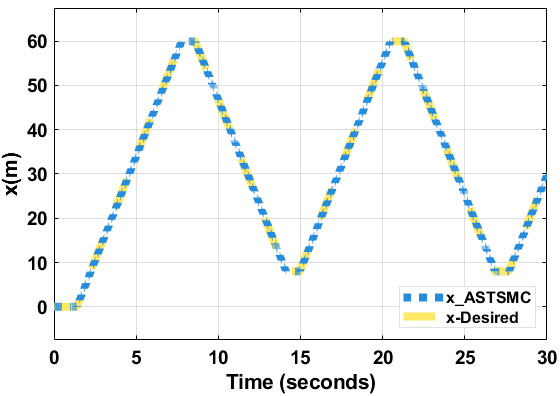
\includegraphics[width=\linewidth]{figures/x-square wave trajectory.png}
        \caption{Square wave X Position Tracking }
        %\label{fig:x square wave  }
        \label{fig:x square wave tracking}
    \end{minipage}
    \hfill
    \begin{minipage}{0.48\linewidth}
        \centering
        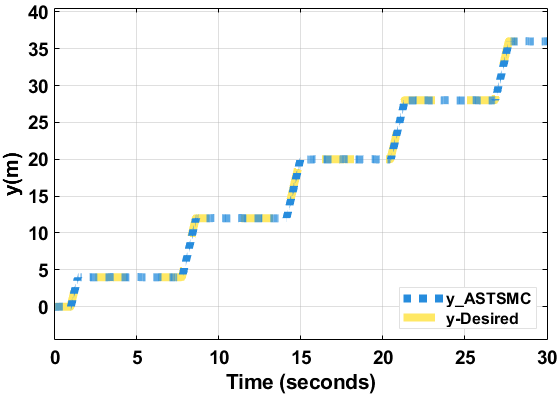
\includegraphics[width=\linewidth]{figures/y-square wave trajectory.png}
        \caption{Square wave Y Position Tracking }
        %\label{fig:square wave y }
        \label{fig:square wave tracking y}
    \end{minipage}
%\end{figure}
  \hfill
    \begin{minipage}{0.48\linewidth}
        \centering
        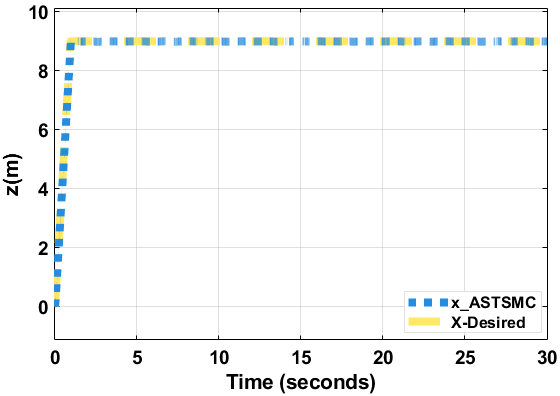
\includegraphics[width=\linewidth]{figures/z-square wave trajectory.png}
        \caption{Square wave Z Position Tracking }
        %\label{fig:z square wave tracking }
        \label{fig:z wave tracking}
    \end{minipage}
%\end{figure}
\hfill
    \begin{minipage}{0.48\linewidth}
        \centering
        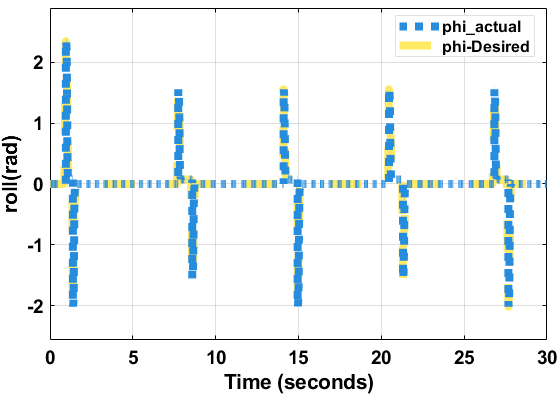
\includegraphics[width=\linewidth]{figures/roll-square wave trajectory.png}
        \caption{Square wave Roll Angle Tracking }
        %\label{fig:roll square wave tracking }
        \label{fig:roll square wave tracking}
    \end{minipage}
    \hfill
    \begin{minipage}{0.48\linewidth}
        \centering
        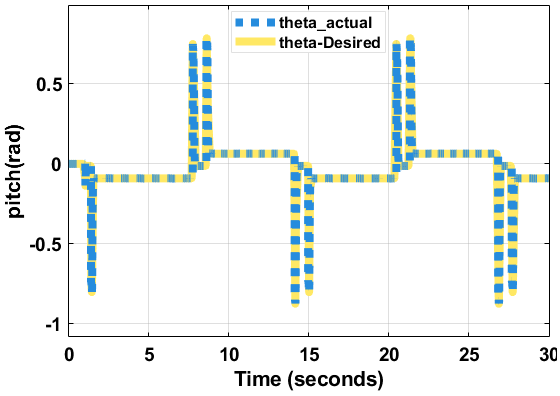
\includegraphics[width=\linewidth]{figures/pitch-square wave trajectory.png}
        \caption{Square wave Pitch Angle Tracking }
        %\label{fig:pitch square wave tracking }
        \label{fig:pitch square wave tracking}
    \end{minipage}
  \hfill
    \begin{minipage}{0.48\linewidth}
        \centering
        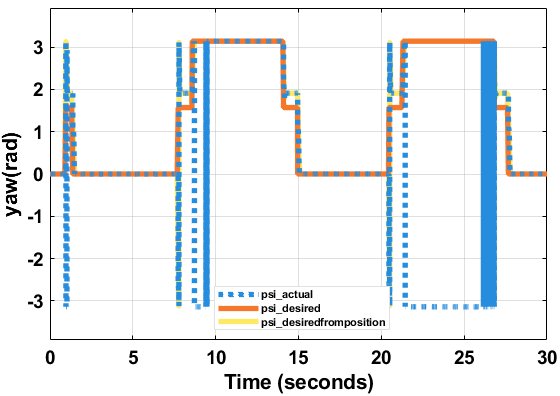
\includegraphics[width=\linewidth]{figures/yaw-square wave trajectory.png}
        \caption{Yaw Square wave tracking }
       % \label{fig:yaw square wave tracking }
       \label{fig:yaw square wave tracking}
    \end{minipage}
\end{figure}


%%%



\begin{figure}[h!]
    \centering
    \begin{minipage}{0.48\linewidth}
        \centering
        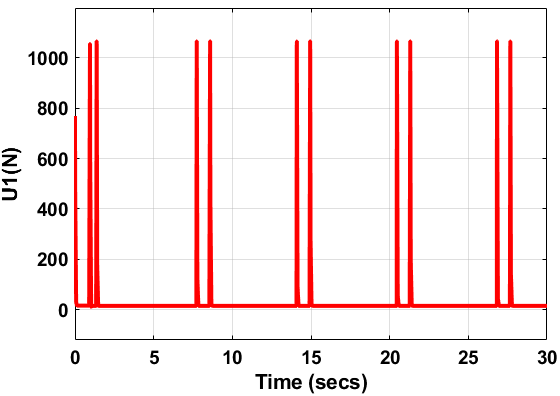
\includegraphics[width=\linewidth]{figures/U1-square wave.png}
        \caption{Control input U1 for square wave trajectory}
        \label{fig:U1 square wave}
    \end{minipage}
    \hfill
    \begin{minipage}{0.48\linewidth}
        \centering
        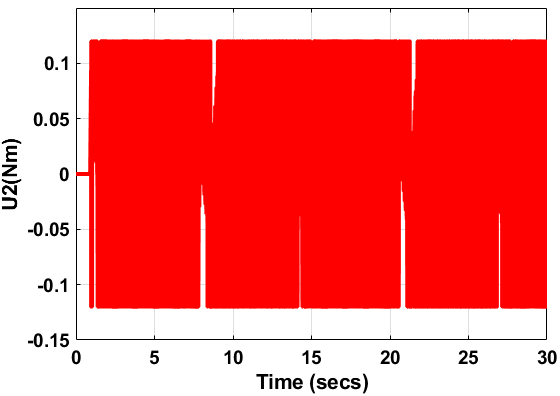
\includegraphics[width=\linewidth]{figures/U2-square wave.png}
        \caption{Control input U2 for square wave trajectory}
        \label{fig:U2 square wave}
    \end{minipage}
%\end{figure}

  \hfill
    \begin{minipage}{0.48\linewidth}
        \centering
        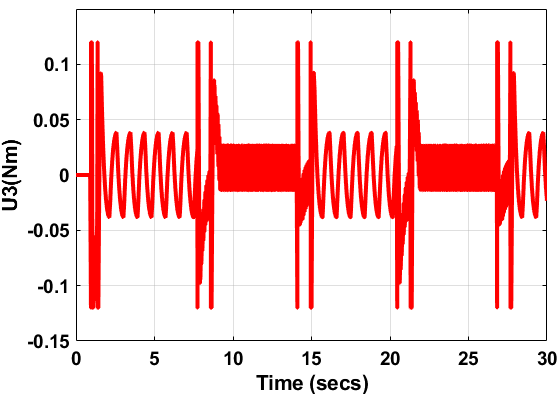
\includegraphics[width=\linewidth]{figures/U3-square wave.png}
        \caption{Control input U3 for square wave trajectory}
        \label{fig:U3 square wave}
    \end{minipage}
%\end{figure}
  \hfill
    \begin{minipage}{0.48\linewidth}
        \centering
        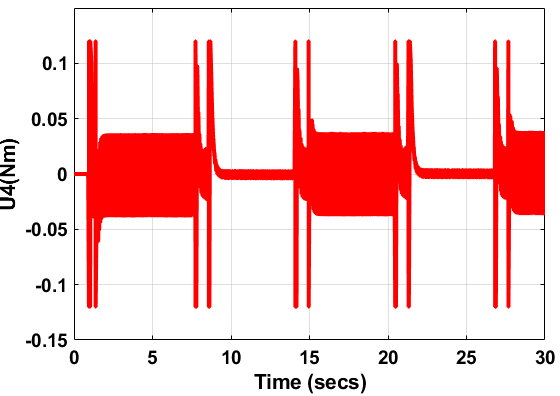
\includegraphics[width=\linewidth]{figures/U4-square wave.png}
        \caption{Control input U4 for square wave trajectory}
        \label{fig:U4 square wave}
    \end{minipage}
\hfill
    \begin{minipage}{0.48\linewidth}
        \centering
        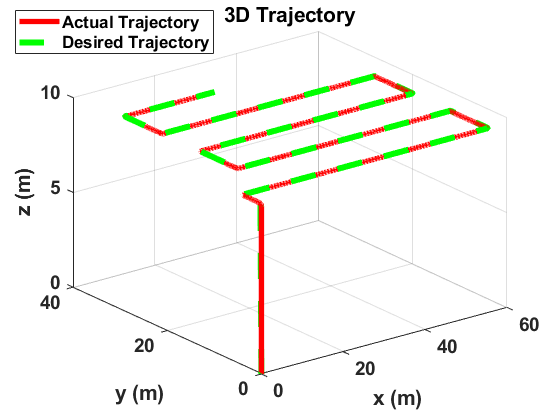
\includegraphics[width=\linewidth]{figures/3D-square wave trajectory.png}
        \caption{Square wave 3D Position Tracking }
        %\label{fig:3D position square wave tracking }
        \label{fig:3D square wave tracking}
    \end{minipage}
    
\end{figure}


				\chapter{CONCLUSIONS \& RECOMMENDATIONS}
%\section*{Conclusion}
%\section*{\center{CONCLUSION}}
%\addcontentsline{toc}{chapter}{ Conclusion}
%\section{Introduction}
%The main conclusions and findings from the research study on the Marshall-Olkin Alpha Power Transformed Extended-Inverted Kumaraswamy distribution are summarized in this chapter. Additionally, it provides recommendations for future potential areas of investigation and makes use of the proposed distribution.
%\section{Summary of Findings}
%This study proposed a novel of  four parameters distribution using  the Marshall-Olkin Alpha Power Transformed Extended-X family of distribution which increase the flexibility and applicability of the Inverted Kumaraswamy Distribution . 
%The  Marshall-Olkin Alpha Power Transformed Extended-X family of distribution is the extension of Alpha Power Transformed Extended-X family of distribution using the Marshall-Olkin method.\\
%The Probability density function, Cumulative density function, survival function and hazard rate function of the MOAPTE-IK are mathematically derived  and graphically presented in this work. 
  
%Maximum Likelihood approach for parameter estimation is used, and the behavior of the resulting estimates was assessed through a Monte Carlo simulation, the performance of the estimators is evaluated using Root Mean Squared Error (RMSE) and bias. \\
%The suggested model was applicable  using two datasets and was compared with the existing models  using selection criteria and goodness-of-fit tests to demonstrate its flexibility.


\section{Conclusions}	
Quadrotor UAV trajectory tracking remains challenging due to highly coupled nonlinear dynamics, parametric uncertainties, and external disturbances. Conventional controllers like PID lack robustness under model mismatches, while classical sliding mode control suffers from chattering and manual gain-tuning difficulties. This research addresses these limitations by developing a Particle Swarm Optimization (PSO) tuned Adaptive Super Twisting Sliding Mode Controller (ASTSMC) based on a quaternion dynamic model that captures unmodeled aerodynamic effects and avoids gimbal lock.

The proposed PSO-ASTSMC achieved remarkable performance improvements: 27\% reduction in attitude errors, 9\% enhancement in position accuracy, and 28--30\% decrease in combined tracking error and control effort. Under 50\% parametric variation (1kg to 1.5kg mass increase), ASTSMC demonstrated exceptional robustness with only 2\% Y-axis degradation compared to Back stepping SMC's catastrophic 97\% failure representing 48.5 times superior performance. The controller achieved 65\% thrust reduction versus PID's 36\%, ensuring energy efficient operation critical for battery powered UAVs.

For disturbance rejection under continuous $d = 1 - \cos(t)$ forcing, ASTSMC maintained 25\% X-axis, 7\% Y-axis, and 20\% Z-axis degradation while back stepping sliding mode controller (BSMC) collapsed with 72--92\% deterioration. The adaptive super twisting mechanism eliminated chattering while maintaining smooth torque profiles, preventing actuator saturation.

This work's novelty lies in synergistically combining PSO optimization with adaptive super twisting control on a realistic quaternion model, achieving parametric invariance, finite time convergence, and superior disturbance attenuation with minimal control expenditure establishing a robust framework for autonomous flight under model uncertainties and environmental disturbances.

	\section{Recommendations}	

\noindent Although the proposed controller was intended for real-time implementation, its deployment on the Carbon Aeronautics platform was not completed due to limitations associated with sensing, estimation, and hardware integration rather than insufficient computational power. The Teensyduino microcontroller provided adequate processing capability for the execution of the quaternion-based adaptive super-twisting sliding mode control algorithm. However, successful hardware implementation required dependable real-time acquisition of attitude, angular rate, altitude, and translational state information, together with robust sensor fusion and actuator-level validation. The Carbon Aeronautics platform, in its available configuration, did not provide the complete measurement and integration framework necessary to support the full controller safely and reliably. Consequently, experimental implementation was deferred, and the controller was assessed in simulation. Future studies should emphasize enhanced sensing, state estimation, and full hardware-software integration to enable practical real-time validation.
    

%\section*{\hspace{5cm}REFERENCES}
%\addcontentsline{toc}{chapter}{Marshall-Olkin}
    %\renewcommand{\bibname}{References}
    %\bibliographystyle{apalike}
    %\bibliography{Marshall-Olkin}
    %\addcontentsline{toc}{chapter}{References}



% ---- References section ----
%\renewcommand{\bibname}{References}   % Works for report/book class

\renewcommand{\bibname}{References}   % Works for report/book class
\bibliographystyle{IEEEtran}          % IEEE style
\bibliography{UAVreferences}
\addcontentsline{toc}{chapter}{REFERENCES}
%\addcontentsline{toc}{chapter}{References}


%\renewcommand{\bibname}{References}
%\bibliographystyle{apalike}
%\bibliography{Marshall-Olkin}
%\newpage
				
%\begin{figure}
\newpage
\section*{\center{APPENDICES}}
\addcontentsline{toc}{chapter}{APPENDIX}

\appendix
% Redefine section and equation numbering for appendices
%\renewcommand{\thesection}{\Alph{section}}
%\renewcommand{\theequation}{\thesection.\arabic{equation}}

%\section{APPENDIX A: Github link for the PSO Algorithm in MATLAB}
%\setcounter{equation}{0} 
%https://github.com/MUSA1994DAUD/PSO-optimization


%%%%%%%%trial%%%%%%%%%%%%%%%%%%

%%%%%%%%%%%%5
\appendix
\setcounter{section}{0}
\renewcommand{\thesection}{\arabic{section}}

\section{APPENDIX A: Github link for the PSO Algorithm in MATLAB}
\addappendix{APPENDIX A: Github link for the PSO Algorithm in MATLAB}

\setcounter{equation}{0}
\url{https://github.com/MUSA1994DAUD/PSO-optimization}

\vspace{1cm}

\section{APPENDIX B: Github link for designed controller in MATLAB/Simulink}
\addappendix{APPENDIX B: Github link for designed controller in MATLAB/Simulink}

\setcounter{equation}{0}
%\url{https://github.com/MUSA1994DAUD/Adaptive-super-twisting-sliding-mode-controller-for-quadcopter}
%\usepackage{hyperref} % in preamble


\href{https://github.com/MUSA1994DAUD/Adaptive-super-twisting-sliding-mode-controller-for-quadcopter}{ASTSMC Quadcopter GitHub Repository}


\\\\
 %\newpage
   %\section{APPENDIX B:Github link for designed controller in MATLAB/Simulink}
 %\setcounter{equation}{0}
 %https://github.com/MUSA1994DAUD/Adaptive-super-twisting-sliding-mode-controller-for-quadcopter
 
%\section*{APPENDIX C}
%\textbf{\large PUBLICATION}\\\\
%https://doi.org/10.28919/cmbn/9055\\
%Eunice Shadrack John, Anthony Kibira Wanjoya, Mutua Kilai, "Marshall-Olkin alpha power transformed extended exponential distribution", Commun. Math. Biol. Neurosci., 2025 (2025), Article ID 17
%\includegraphics[width=420pt, height=240pt]{WORK PLAN}
%\label{tab:Work plan}
%\end{figure}
%\chapter{APPENDIX B}
%\section*{Budget}
%\centering
%\begin{table}[h]
%\centering
%\begin{tabular}{|l|r|r|r|}
%\hline
%\textbf{ITEMS} & \textbf{Quantity} & \textbf{Unity cost (\$)} & \textbf{Total cost (\$)} \\ \hline
%Laptop & 1  & 600 & 600  \\ \hline % use \cellcolor to colour a single cell
%Data Acquisition &   &  & 500 \\ \hline
%Photocopy, printing and binding
%&   &  & 300 \\ \hline
%Internet bundle & 6 months   & 40   & 240  \\ \hline
%Conferences and workshops
%& 1  & 400  & 400  \\ \hline
%Reference books
%& 3  & 110   & 220   \\ \hline
%Publication fee & 1  & 600   & 600  \\ \hline % use another colour for a different cell
%Miscellaneous
%&   &   & 100  \\ \hline
%\cellcolor{cyan}\textbf{TOTAL}  & 	\cellcolor{cyan}  & 	\cellcolor{cyan}  & 	\cellcolor{cyan}\textbf{2960}  \\ \hline
%\end{tabular}
%\label{fig:Budget}
%\end{table}
\end{document}